% Options for packages loaded elsewhere
\PassOptionsToPackage{unicode}{hyperref}
\PassOptionsToPackage{hyphens}{url}
\PassOptionsToPackage{dvipsnames,svgnames,x11names}{xcolor}
%
\documentclass[
  letterpaper,
  11pt,
  english,
  singlespacing,
  headsepline]{MastersDoctoralThesis}

\usepackage{amsmath,amssymb}
\usepackage{iftex}
\ifPDFTeX
  \usepackage[T1]{fontenc}
  \usepackage[utf8]{inputenc}
  \usepackage{textcomp} % provide euro and other symbols
\else % if luatex or xetex
  \usepackage{unicode-math}
  \defaultfontfeatures{Scale=MatchLowercase}
  \defaultfontfeatures[\rmfamily]{Ligatures=TeX,Scale=1}
\fi
\usepackage{lmodern}
\ifPDFTeX\else  
    % xetex/luatex font selection
\fi
% Use upquote if available, for straight quotes in verbatim environments
\IfFileExists{upquote.sty}{\usepackage{upquote}}{}
\IfFileExists{microtype.sty}{% use microtype if available
  \usepackage[]{microtype}
  \UseMicrotypeSet[protrusion]{basicmath} % disable protrusion for tt fonts
}{}
\makeatletter
\@ifundefined{KOMAClassName}{% if non-KOMA class
  \IfFileExists{parskip.sty}{%
    \usepackage{parskip}
  }{% else
    \setlength{\parindent}{0pt}
    \setlength{\parskip}{6pt plus 2pt minus 1pt}}
}{% if KOMA class
  \KOMAoptions{parskip=half}}
\makeatother
\usepackage{xcolor}
\usepackage[paper=a4paper,inner=2.5cm,outer=3.8cm,bindingoffset=.5cm,top=1.5cm,bottom=1.5cm]{geometry}
\setlength{\emergencystretch}{3em} % prevent overfull lines
\setcounter{secnumdepth}{5}
% Make \paragraph and \subparagraph free-standing
\makeatletter
\ifx\paragraph\undefined\else
  \let\oldparagraph\paragraph
  \renewcommand{\paragraph}{
    \@ifstar
      \xxxParagraphStar
      \xxxParagraphNoStar
  }
  \newcommand{\xxxParagraphStar}[1]{\oldparagraph*{#1}\mbox{}}
  \newcommand{\xxxParagraphNoStar}[1]{\oldparagraph{#1}\mbox{}}
\fi
\ifx\subparagraph\undefined\else
  \let\oldsubparagraph\subparagraph
  \renewcommand{\subparagraph}{
    \@ifstar
      \xxxSubParagraphStar
      \xxxSubParagraphNoStar
  }
  \newcommand{\xxxSubParagraphStar}[1]{\oldsubparagraph*{#1}\mbox{}}
  \newcommand{\xxxSubParagraphNoStar}[1]{\oldsubparagraph{#1}\mbox{}}
\fi
\makeatother


\providecommand{\tightlist}{%
  \setlength{\itemsep}{0pt}\setlength{\parskip}{0pt}}\usepackage{longtable,booktabs,array}
\usepackage{calc} % for calculating minipage widths
% Correct order of tables after \paragraph or \subparagraph
\usepackage{etoolbox}
\makeatletter
\patchcmd\longtable{\par}{\if@noskipsec\mbox{}\fi\par}{}{}
\makeatother
% Allow footnotes in longtable head/foot
\IfFileExists{footnotehyper.sty}{\usepackage{footnotehyper}}{\usepackage{footnote}}
\makesavenoteenv{longtable}
\usepackage{graphicx}
\makeatletter
\newsavebox\pandoc@box
\newcommand*\pandocbounded[1]{% scales image to fit in text height/width
  \sbox\pandoc@box{#1}%
  \Gscale@div\@tempa{\textheight}{\dimexpr\ht\pandoc@box+\dp\pandoc@box\relax}%
  \Gscale@div\@tempb{\linewidth}{\wd\pandoc@box}%
  \ifdim\@tempb\p@<\@tempa\p@\let\@tempa\@tempb\fi% select the smaller of both
  \ifdim\@tempa\p@<\p@\scalebox{\@tempa}{\usebox\pandoc@box}%
  \else\usebox{\pandoc@box}%
  \fi%
}
% Set default figure placement to htbp
\def\fps@figure{htbp}
\makeatother
% definitions for citeproc citations
\NewDocumentCommand\citeproctext{}{}
\NewDocumentCommand\citeproc{mm}{%
  \begingroup\def\citeproctext{#2}\cite{#1}\endgroup}
\makeatletter
 % allow citations to break across lines
 \let\@cite@ofmt\@firstofone
 % avoid brackets around text for \cite:
 \def\@biblabel#1{}
 \def\@cite#1#2{{#1\if@tempswa , #2\fi}}
\makeatother
\newlength{\cslhangindent}
\setlength{\cslhangindent}{1.5em}
\newlength{\csllabelwidth}
\setlength{\csllabelwidth}{3em}
\newenvironment{CSLReferences}[2] % #1 hanging-indent, #2 entry-spacing
 {\begin{list}{}{%
  \setlength{\itemindent}{0pt}
  \setlength{\leftmargin}{0pt}
  \setlength{\parsep}{0pt}
  % turn on hanging indent if param 1 is 1
  \ifodd #1
   \setlength{\leftmargin}{\cslhangindent}
   \setlength{\itemindent}{-1\cslhangindent}
  \fi
  % set entry spacing
  \setlength{\itemsep}{#2\baselineskip}}}
 {\end{list}}
\usepackage{calc}
\newcommand{\CSLBlock}[1]{\hfill\break\parbox[t]{\linewidth}{\strut\ignorespaces#1\strut}}
\newcommand{\CSLLeftMargin}[1]{\parbox[t]{\csllabelwidth}{\strut#1\strut}}
\newcommand{\CSLRightInline}[1]{\parbox[t]{\linewidth - \csllabelwidth}{\strut#1\strut}}
\newcommand{\CSLIndent}[1]{\hspace{\cslhangindent}#1}

\usepackage[utf8]{inputenc} % Required for inputting international characters
%\usepackage[T1]{fontenc} % Output font encoding for international characters; causes problems for xelatex

%\usepackage{mathpazo} % Use the Palatino font by default

\usepackage[backend=bibtex, style=authoryear, natbib=true]{biblatex} % Use the bibtex backend with the authoryear citation style (which resembles APA)

\usepackage[autostyle=true]{csquotes} % Required to generate language-dependent quotes in the bibliography

\usepackage{setspace}

\usepackage{tikz}
\usetikzlibrary{calc}
\usetikzlibrary{calc,decorations.pathmorphing}
\usepackage{tocloft}
\usepackage{lscape} % For landscape pages
\usepackage{geometry} % For custom page layout
\usepackage{graphicx} % For including images
\usepackage{caption} % For custom captions
\usepackage{truncate}
\usepackage{lipsum} % For dummy text
\usepackage{xcolor} % To define and use colors
\usepackage{eso-pic} % For background images % For including images
\definecolor{textgray}{HTML}{595959}
\definecolor{greenTriangle}{HTML}{1f7549}
\definecolor{greenText}{HTML}{2DA86A}
\usepackage{tikz} % Load the TikZ package
\usepackage{tabularx}
\usepackage{fontspec} % To use system fonts like Arial
\PassOptionsToPackage{scaled}{helvet}
\usepackage{helvet}
\usetikzlibrary{patterns,patterns.meta} % LaTeX and plain TeX when using TikZ
\usepackage{titlesec}
\titleformat{\paragraph}[runin]{\normalfont\normalsize\bfseries}{\theparagraph}{1em}{}
\usepackage{multicol}
\usepackage{changepage}
%----------------------------------------------------------------------------------------
%	MARGINS
%----------------------------------------------------------------------------------------

\geometry{
	headheight=4ex,
	includehead,
	includefoot
}

\raggedbottom

\AtBeginDocument{
\hypersetup{pdftitle=\ttitle} % Set the PDF's title to your title
\hypersetup{pdfauthor=\authorname} % Set the PDF's author to your name
\hypersetup{pdfkeywords=\keywordnames} % Set the PDF's keywords to your keywords
}

\usepackage{tcolorbox}
\tcbset{
  colback=gray!10, % Background color (10% grey)
  colframe=gray!50, % Border color (50% grey)
  boxrule=0.5mm, % Border thickness
  arc=4mm, % Border radius
  left=1mm, % Left padding
  right=1mm, % Right padding
  top=1mm, % Top padding
  bottom=1mm, % Bottom padding
}

\renewcommand{\floatpagefraction}{0.8} % Allow floats to occupy up to 80% of a page
\renewcommand{\textfraction}{0.1}     % Allow text to occupy as little as 10% of a page
\renewcommand{\topfraction}{0.9}      % Allow up to 90% of the top of a page for floats
\renewcommand{\bottomfraction}{0.9}   % Allow up to 90% of the bottom of a page for floats

\newcommand{\startonrightwithgap}{%
  \clearpage
  % Check whether the current page is odd
  \ifodd\value{page}
    % -- We are on odd page X, so skip two pages (X+1, X+2):
    \thispagestyle{empty}\mbox{}\clearpage
    \thispagestyle{empty}\mbox{}\clearpage
  \else
    % -- We are on even page Y, so skip one page (Y+1):
    \thispagestyle{empty}\mbox{}\clearpage
  \fi
}

\newcommand{\startonleftwithgap}{%
  \clearpage
  \ifodd\value{page}
    % If the current page is odd, skip 3 blank pages
    \thispagestyle{empty}\mbox{}\clearpage
    \thispagestyle{empty}\mbox{}\clearpage
    \thispagestyle{empty}\mbox{}\clearpage
  \else
    % If the current page is even, skip 2 blank pages
    \thispagestyle{empty}\mbox{}\clearpage
    \thispagestyle{empty}\mbox{}\clearpage
  \fi
}
% 
% \newcommand{\startonrightwithgap}{%
%   \clearpage % End the current section cleanly
%   \ifodd\value{page} % Check if the current page is odd
%     \null\newpage % Add a blank page if odd
%     \thispagestyle{empty} % Ensure the blank page has no headers/footers
%   \else
%     \null\newpage % Add a blank page if even (this ensures X+1 is blank)
%     \thispagestyle{empty} % Ensure the blank page has no headers/footers
%     \null\newpage % Add another blank page for X+2
%     \thispagestyle{empty} % Ensure this blank page has no headers/footers
%   \fi
%   \cleardoublepage % Ensure the next section starts on a right (odd) page
% }

\newcommand{\chaptertopimage}{Chapter1/img/seagrasses.png}
\newcommand{\chapterbottomimage}{Chapter1/img/seagrasses.png}

\newcommand{\chaptertransition}{
    \clearpage
    \thispagestyle{empty}
    \null
    \newpage
}

\usepackage{geometry}  % presumably already in your preamble
% ... your usual margin setup, e.g.:
% \geometry{margin=1in}

\newcommand{\chaptertitlepage}[4]{%
  \chaptertransition
  \thispagestyle{empty}

  % Temporarily remove margins:
  \newgeometry{margin=0pt}

  \begin{center}
    % Top image, spanning full page width
    \includegraphics[width=\paperwidth]{#1}

    \vfill

    % Chapter number and title:
    {\Huge \textbf{Chapter #2: \\#3}}

    \vfill

    % Bottom image, also spanning full page width
    \includegraphics[width=\paperwidth]{#4}
  \end{center}

  % Restore your normal geometry:
  \restoregeometry
}

\usepackage{fontspec}
\usepackage{multirow}
\usepackage{multicol}
\usepackage{colortbl}
\usepackage{hhline}
\newlength\Oldarrayrulewidth
\newlength\Oldtabcolsep
\usepackage{longtable}
\usepackage{array}
\usepackage{hyperref}
\usepackage{float}
\usepackage{wrapfig}
\makeatletter
\@ifpackageloaded{bookmark}{}{\usepackage{bookmark}}
\makeatother
\makeatletter
\@ifpackageloaded{caption}{}{\usepackage{caption}}
\AtBeginDocument{%
\ifdefined\contentsname
  \renewcommand*\contentsname{Table of contents}
\else
  \newcommand\contentsname{Table of contents}
\fi
\ifdefined\listfigurename
  \renewcommand*\listfigurename{List of Figures}
\else
  \newcommand\listfigurename{List of Figures}
\fi
\ifdefined\listtablename
  \renewcommand*\listtablename{List of Tables}
\else
  \newcommand\listtablename{List of Tables}
\fi
\ifdefined\figurename
  \renewcommand*\figurename{Figure}
\else
  \newcommand\figurename{Figure}
\fi
\ifdefined\tablename
  \renewcommand*\tablename{Table}
\else
  \newcommand\tablename{Table}
\fi
}
\@ifpackageloaded{float}{}{\usepackage{float}}
\floatstyle{ruled}
\@ifundefined{c@chapter}{\newfloat{codelisting}{h}{lop}}{\newfloat{codelisting}{h}{lop}[chapter]}
\floatname{codelisting}{Listing}
\newcommand*\listoflistings{\listof{codelisting}{List of Listings}}
\makeatother
\makeatletter
\makeatother
\makeatletter
\@ifpackageloaded{caption}{}{\usepackage{caption}}
\@ifpackageloaded{subcaption}{}{\usepackage{subcaption}}
\makeatother

\usepackage{bookmark}

\IfFileExists{xurl.sty}{\usepackage{xurl}}{} % add URL line breaks if available
\urlstyle{same} % disable monospaced font for URLs
\hypersetup{
  pdftitle={Caractérisation par télédétection multi-échelle de la végétation intertidale des côtes européennes en réponses aux pressions naturelles et anthropiques},
  pdfauthor={Simon Oiry},
  colorlinks=true,
  linkcolor={black},
  filecolor={Maroon},
  citecolor={black},
  urlcolor={black},
  pdfcreator={LaTeX via pandoc}}


\thesistitle{Caractérisation par télédétection multi-échelle de la
végétation intertidale des côtes européennes en réponses aux pressions
naturelles et
anthropiques} % Your thesis title, this is used in the title and abstract, print it elsewhere with \ttitle

% Modified section for multiple supervisors
\supervisor{Prof.~Laurent Barillé, Dr.~Pierre
Gernez} % Your supervisors' names, this will print all listed supervisors

\examiner{} % Your examiner's name, this is not currently used anywhere in the template, print it elsewhere with \examname
\degree{Doctor of Philosophy in Marine
Ecology} % Your degree name, this is used in the title page and abstract, print it elsewhere with \degreename
\author{Simon
Oiry} % Your name, this is used in the title page and abstract, print it elsewhere with \authorname
\addresses{} % Your address, this is not currently used anywhere in the template, print it elsewhere with \addressname

\subject{} % Your subject area, this is not currently used anywhere in the template, print it elsewhere with \subjectname
\keywords{} % Keywords for your thesis, this is not currently used anywhere in the template, print it elsewhere with \keywordnames
\university{University of
Nantes} % Your university's name, this is used in the title page and abstract, print it elsewhere with \univname
\department{Institut Des Substances et Organismes de la
Mer} % Your department's name, this is used in the title page and abstract, print it elsewhere with \deptname
\group{Remote Sensing, Benthic Ecology and Ecotoxicology
team} % Your research group's name and URL, this is used in the title page, print it elsewhere with \groupname
\faculty{Sciences \&
Techniques} % Your faculty's name and URL, this is used in the title page and abstract, print it elsewhere with \facname

\setcounter{tocdepth}{3} % The depth to which the document sections are printed to the table of contents
\begin{document}
%----------------------------------------------------------------------------------------
% FRONT MATTER CONFIGURATION
% Using roman page numbering style (i, ii, iii, iv...) for the pre-content pages
%----------------------------------------------------------------------------------------
\frontmatter

% Default to the plain heading style until the thesis style is called for the body content
\pagestyle{plain}

%----------------------------------------------------------------------------------------
% TITLE PAGE
%----------------------------------------------------------------------------------------
\newgeometry{top=0.5in, bottom=0.5in, left=0.5in, right=0.5in}

\begin{titlepage}

% Use Helvetica (Arial substitute)
\renewcommand{\familydefault}{\sfdefault}


\newcommand\BackgroundImage{%
    \put(0,3.5cm){%
        \parbox[b][\paperheight]{\paperwidth}{%
            \vfill
            \includegraphics[width=\paperwidth]{Backgound_First_Page.png} % Replace with your image
            \vfill
        }%
    }%
}

% Use Arial font for the title page
\setsansfont{Arial}

\begin{tabularx}{\textwidth}{X X} % Two equally spaced columns
  \centering\includegraphics[height=2cm]{LogoED.png} & 
  \centering\includegraphics[height=2cm]{LogoUN.jpg} \\
\end{tabularx}

% Add the background image
\AddToShipoutPictureBG*{%
    \BackgroundImage
}

\vspace{1.2cm}

% Custom font sizes for "THESE DE DOCTORAT"
{\LARGE {\Huge T}HESE DE DOCTORAT}

\vspace{1.8cm}
% Custom font sizes for "NANTES UNIVERSITE"
{\fontsize{14}{18}\selectfont NANTES UNIVERSITE} \\

{\large E}COLE {\large D}OCTORALE N° 642


{\fontsize{12}{16}\selectfont \textit{Ecole doctorale Végétal, Animal, Aliment, Mer, Environnement}}

{\fontsize{12}{16}\selectfont Spécialité : Biologie et écologie marine} \\\\\\

{\fontsize{12}{16}\ Par}
\vspace{0.2cm}

\hspace{0.7cm}{\fontsize{20}{24}\selectfont \textbf{Simon OIRY}} \\

\parbox{17cm}{
{\fontsize{16}{20}\selectfont \textbf{Caractérisation par télédétection multi-échelle de la végétation intertidale des côtes européennes en réponses aux pressions naturelles et anthropiques} }
}\\\\

{\fontsize{11}{15}\selectfont \textbf{Thèse présentée et soutenue à Nantes, le 15 mai 2025}}

{\fontsize{11}{15}\selectfont \textbf{Unité de Recherche: Institut Des Substances et Organismes de la Mer}}
\\\\\\

{\fontsize{12}{16}\selectfont \textbf{Rapporteurs avant soutenance :}}

\begin{tabular}{@{}l l l@{}}
    {\fontsize{10}{14}\selectfont \textcolor{textgray}{Antoine Collin}} & 
    {\fontsize{10}{14}\selectfont \textcolor{textgray}{Maitre de conférences}} & 
    {\fontsize{10}{14}\selectfont \textcolor{textgray}{Ecole Pratique des Hautes Etudes, Dinard}} \\

    {\fontsize{10}{14}\selectfont \textcolor{textgray}{Rodney Foster}} & 
    {\fontsize{10}{14}\selectfont \textcolor{textgray}{Professeur}} & 
    {\fontsize{10}{14}\selectfont \textcolor{textgray}{Université de Hull, Royaume-Uni}} \\
\end{tabular}\\\\

{\fontsize{12}{16}\selectfont \textbf{Composition du Jury : }}

\begin{tabular}{@{}l l l l@{}}
    {\fontsize{10}{14}\selectfont \textcolor{textgray}{Président :}} & 
    {\fontsize{10}{14}\selectfont \textcolor{textgray}{ }} & 
    {\fontsize{10}{14}\selectfont \textcolor{textgray}{ }} & 
    {\fontsize{10}{14}\selectfont \textcolor{textgray}{ }} \\

    {\fontsize{10}{14}\selectfont \textcolor{textgray}{Examinateurs :}} & 
    {\fontsize{10}{14}\selectfont \textcolor{textgray}{Antoine Collin}} & 
    {\fontsize{10}{14}\selectfont \textcolor{textgray}{Maitre de conférences}} & 
    {\fontsize{10}{14}\selectfont \textcolor{textgray}{Ecole Pratique des Hautes Etudes, Dinard}} \\
    
    {\fontsize{10}{14}\selectfont \textcolor{textgray}{}} & 
    {\fontsize{10}{14}\selectfont \textcolor{textgray}{Rodney Foster}} & 
    {\fontsize{10}{14}\selectfont \textcolor{textgray}{Professeur}} & 
    {\fontsize{10}{14}\selectfont \textcolor{textgray}{Université de Hull, Royaume-Uni}} \\

    {\fontsize{10}{14}\selectfont \textcolor{textgray}{}} & 
    {\fontsize{10}{14}\selectfont \textcolor{textgray}{Evangelos Spyrakos}} & 
    {\fontsize{10}{14}\selectfont \textcolor{textgray}{Professeur}} & 
    {\fontsize{10}{14}\selectfont \textcolor{textgray}{Université de Stirling, Royaume-Uni}} \\

    {\fontsize{10}{14}\selectfont \textcolor{textgray}{}} & 
    {\fontsize{10}{14}\selectfont \textcolor{textgray}{Barbara Ondiviela}} & 
    {\fontsize{10}{14}\selectfont \textcolor{textgray}{Senior scientist}} & 
    {\fontsize{10}{14}\selectfont \textcolor{textgray}{Université de Cantabrie, Espagne}} \\

    {\fontsize{10}{14}\selectfont \textcolor{textgray}{Dir. de thèse :}} & 
    {\fontsize{10}{14}\selectfont \textcolor{textgray}{Laurent Barillé}} & 
    {\fontsize{10}{14}\selectfont \textcolor{textgray}{Professeur}} & 
    {\fontsize{10}{14}\selectfont \textcolor{textgray}{Nantes Université}} \\

    {\fontsize{10}{14}\selectfont \textcolor{textgray}{Co-dir. de thèse :}} & 
    {\fontsize{10}{14}\selectfont \textcolor{textgray}{Pierre Gernez}} & 
    {\fontsize{10}{14}\selectfont \textcolor{textgray}{Maitre de conférence}} & 
    {\fontsize{10}{14}\selectfont \textcolor{textgray}{Nantes Université}} \\
\end{tabular} \\\\

{\fontsize{11}{15}\selectfont \textbf{Invitée : }}


\begin{tabular}{@{}l l l@{}}
    {\fontsize{10}{14}\selectfont \textcolor{textgray}{Federica Braga}} & 
    {\fontsize{10}{14}\selectfont \textcolor{textgray}{Senior Researcher}} & 
    {\fontsize{10}{14}\selectfont \textcolor{textgray}{Conseil Supérieur de la Recherche, Venise, Italie}} \\

\end{tabular}
\end{titlepage}

% Restore the default margins for the rest of the document
\restoregeometry

% Reset to serif font for the rest of the document
\renewcommand{\familydefault}{\rmdefault}


%----------------------------------------------------------------------------------------
% DECLARATION PAGE
%----------------------------------------------------------------------------------------

%----------------------------------------------------------------------------------------
% QUOTATION PAGE (IF ANY)
%----------------------------------------------------------------------------------------

%----------------------------------------------------------------------------------------
% ABSTRACT PAGE
%----------------------------------------------------------------------------------------
% %   \clearpage
%   \begin{abstract}
%     \addchaptertocentry{\abstractname}  % Add the abstract to the table of contents
%     To Be Written
%   \end{abstract}
% 
%----------------------------------------------------------------------------------------
% ACKNOWLEDGEMENTS
%----------------------------------------------------------------------------------------
  \startonrightwithgap
  \begin{acknowledgements}
    \addchaptertocentry{\acknowledgementname} % Add the acknowledgements to the table of contents
          

Ce parcours de doctorat a été long, difficile et parfois épuisant, mais il a également été rempli de moments enrichissants et de personnes incroyables qui ont rendu tout cela digne d'intérêt.

Tout d'abord, je tiens à exprimer ma plus profonde gratitude à mon directeur de thèse, Laurent Barillé. Merci pour tes conseils, ta patience et ton soutien sans faille tout au long de ce processus. Merci pour toute la liberté que tu m'as accordée pendant ces années. Ton expertise et tes encouragements m'ont poussé à m'améliorer à chaque étape, même lorsque j'avais des doutes. J'ai appris énormément sous ta direction, et je suis vraiment reconnaissant de la confiance que tu m'as accordée. Un merci particulier pour ton aide avec toutes les démarches administratives — je sais que j'ai été paresseux à ce sujet, et j'apprécie sincèrement ta patience !

Un grand merci également à mon co-directeur, Pierre Gernez, pour tes conseils avisés, tes retours constructifs et ton soutien constant. Ta perspective m'a toujours aidé à prendre du recul et à voir les choses plus clairement, et j'ai profondément apprécié nos discussions.

J'ai eu une chance incroyable de travailler aux côtés de Bede Davies, dont la générosité en termes de temps et de connaissances a dépassé tout ce que j'aurais pu espérer d'un collègue. Bede, collaborer avec toi a été l'un des meilleurs aspects de ce doctorat — ta patience et ton dévouement ont rendu même les défis de recherche les plus difficiles plus faciles à gérer.

Je tiens également à remercier sincèrement Philippe Rosa, qui a été un véritable sauveur pendant les travaux de terrain. Philippe, tu étais toujours là, prêt à aider, résoudre des problèmes ou simplement partager un éclat de rire quand les choses allaient inévitablement de travers sur le terrain.

Sur un plan plus personnel, je dois une immense gratitude à Laura Zoffoli. Merci d'avoir supporté les nuits tardives, le stress et les conversations interminables sur les herbiers et la télédétection. Ton soutien et ta patience ont été essentiels pour moi, et je n'aurais pas pu accomplir cela sans toi.

Enfin, à ma famille — merci de m'avoir toujours cru, même lorsque je ne croyais pas en moi. Vos encouragements, votre amour et vos rappels qu'il y a une vie en dehors de la recherche ont été une source constante de force. Je suis tellement chanceux de vous avoir à mes côtés.

À tous ceux qui ont fait partie de ce parcours d'une manière ou d'une autre — merci.


      \end{acknowledgements}

%----------------------------------------------------------------------------------------
% LIST OF CONTENTS/FIGURES/TABLES
%----------------------------------------------------------------------------------------
\setlength{\cftsecindent}{0.5em}        % Less indentation for sections
\setlength{\cftsubsecindent}{1em}       % Less indentation for subsections
\setlength{\cftsubsubsecindent}{1.5em}  % Less indentation for subsubsections
\renewcommand{\cftfigpresnum}{Figure~}
\renewcommand{\cfttabpresnum}{Table~}
\renewcommand{\cftfigaftersnum}{:~}  % Add ": " after the figure number
\renewcommand{\cfttabaftersnum}{:~}  % Add ": " after the table number  % Prefix for tables
\setlength{\cftbeforefigskip}{0.5em}  % Space between figure entries
\setlength{\cftbeforetabskip}{0.5em} % Space between table entries
\setlength{\cftfignumwidth}{5em} % Adjust width for figure numbers
\setlength{\cfttabnumwidth}{5em} % Adjust width for table numbers
\setlength{\cftfigindent}{0em}    % Indentation for figure captions
\setlength{\cfttabindent}{0em}    % Indentation for table captions
\startonrightwithgap
\begingroup
\hypersetup{linkcolor=black}
\startonrightwithgap
\tableofcontents  
\startonrightwithgap
\listoffigures
\startonrightwithgap
\listoftables 
\endgroup

%----------------------------------------------------------------------------------------
% ABBREVIATIONS (IF ANY)
%----------------------------------------------------------------------------------------
  % \addchaptertocentry{\abbreviationsname}
  % \label{abbreviations}
  \startonrightwithgap
  \input{"Frontmatter/abbreviations.tex"}

%----------------------------------------------------------------------------------------
% PHYSICAL CONSTANTS/OTHER DEFINITIONS (IF ANY)
%----------------------------------------------------------------------------------------

%----------------------------------------------------------------------------------------
% SYMBOLS (IF ANY)
%----------------------------------------------------------------------------------------
  % \addchaptertocentry{\symbolsname}
  \startonrightwithgap
  \input{"Frontmatter/symbols.tex"}

%----------------------------------------------------------------------------------------
% DEDICATION (IF ANY)
%----------------------------------------------------------------------------------------

%----------------------------------------------------------------------------------------
% MAIN CONTENT
%----------------------------------------------------------------------------------------
\mainmatter % Begin numeric (1,2,3...) page numbering
% Return the page headers back to the "thesis" style
\pagestyle{thesis}
% Define some commands to keep the formatting separated from the content 
\newcommand{\keyword}[1]{\textbf{#1}}
\newcommand{\tabhead}[1]{\textbf{#1}}
\newcommand{\code}[1]{\texttt{#1}}
\newcommand{\file}[1]{\texttt{\bfseries#1}}
\newcommand{\option}[1]{\texttt{\itshape#1}}
% \renewcommand{\chaptermark}[1]{\markboth{#1}{}}


\bookmarksetup{startatroot}

\chapter*{Preface}\label{preface}
\addcontentsline{toc}{chapter}{Preface}

\markboth{Preface}{Preface}

This PhD work was carried out at Nantes University between 2022 and
2024, within the ``Remote Sensing, Benthic Ecology and Ecotoxicology''
(RSBE²) team of the Institute of Marine Substances and Organisms
(ISOMer). This thesis was funded by the Ministry of Research and Higher
Education and supervised by the doctoral school ``Plant, Animal, Food,
Sea, Environment'' (VAAME).

\section*{Scientific papers}\label{scientific-papers}
\addcontentsline{toc}{section}{Scientific papers}

\markright{Scientific papers}

\begin{itemize}
\item
  \textbf{Oiry, S}., Davies, B. F. R., Rosa, P., Debly, A., Zoffoli, M.
  L., Barillé, A.-L., Harin, N., Román, M., Gernez, P., \& Barillé, L.
  (Submitted). Heatwave impacts on intertidal seagrass reflectance: From
  laboratory experiment to satellite mapping of Seagrass Heat Shock
  Index.
\item
  \textbf{Oiry, S.}, Davies, B. F. R., Stiger-Pouvreau, V., Gernez, P.,
  \& Barillé, L. (Submitted). Mapping the distribution of the alien
  invasive \emph{Gracilaria vermiculophylla} at the site of its First
  European Observation.
\item
  Barillé, L., Paterson, I. L. R., \textbf{Oiry, S.}, Aris, A.,
  Cook-Cottier, E. J., \& Nurdin, N. (2025). Variability of
  \emph{Kappaphycus alvarezii} cultivation in South-Sulawesi (Indonesia)
  related to the monsoon shift: Water quality, growth and colour
  quantification. \emph{Aquaculture Reports}, 40, 102557.
  https://doi.org/10.1016/j.aqrep.2024.102557
\item
  \textbf{Oiry, S.}, Davies, B. F. R., Sousa, A. I., Rosa, P., Zoffoli,
  M. L., Brunier, G., Gernez, P., \& Barillé, L. (2024). Discriminating
  Seagrasses from Green Macroalgae in European Intertidal Areas Using
  High-Resolution Multispectral Drone Imagery.~\emph{Remote
  Sensing},~\emph{16}(23), 4383. https://doi.org/10.3390/rs16234383
\item
  Román, A., \textbf{Oiry, S.}, Davies, B. F. R., Rosa, P., Gernez, P.,
  Tovar-Sánchez, A., Navarro, G., Méléder, V., \& Barillé, L. (2024).
  Mapping intertidal microphytobenthic biomass with very high-resolution
  remote sensing imagery in an estuarine system. \emph{Science of The
  Total Environment}, 955, 177025.
  https://doi.org/10.1016/j.scitotenv.2024.177025
\item
  Davies, B. F. R., \textbf{Oiry, S.}, Rosa, P., Zoffoli, M. L., Sousa,
  A. I., Thomas, O. R., Smale, D. A., Austen, M. C., Biermann, L.,
  Attrill, M. J., Roman, A., Navarro, G., Barillé, A.-L., Harin, N.,
  Clewley, D., Martinez-Vicente, V., Gernez, P., \& Barillé, L. (2024).
  Intertidal seagrass extent from Sentinel-2 time-series show distinct
  trajectories in Western Europe. \emph{Remote Sensing of Environment},
  312, 114340. https://doi.org/10.1016/j.rse.2024.114340
\item
  Davies, B. F. R., \textbf{Oiry, S.}, Rosa, P., Zoffoli, M. L., Sousa,
  A. I., Thomas, O. R., Smale, D. A., Austen, M. C., Biermann, L.,
  Attrill, M. J., \& others. (2024). A sentinel watching over
  inter-tidal seagrass phenology across Western Europe and North Africa.
  \emph{Communications Earth \& Environment}, 5(1), 382.
  https://doi.org/10.1038/s43247-024-382
\item
  Nurdin, N., Alevizos, E., Syamsuddin, R., Asis, H., Zainuddin, E. N.,
  Aris, A., \textbf{Oiry, S.}, Brunier, G., Komatsu, T., \& Barillé, L.
  (2023). Precision Aquaculture Drone Mapping of the Spatial
  Distribution of~\emph{Kappaphycus alvarezii}~Biomass and
  Carrageenan.~\emph{Remote Sensing},~\emph{15}(14), 3674.
  https://doi.org/10.3390/rs15143674
\item
  Román, A., Prasyad, H.,\textbf{Oiry, S.}, Davies, B. F. R., Brunier,
  G., \& Barillé, L. (2023). Mapping intertidal oyster farms using
  unmanned aerial vehicles (UAV) high-resolution multispectral data.
  \emph{Estuarine, Coastal and Shelf Science}, 291, 108432.
  https://doi.org/10.1016/j.ecss.2023.108432
\item
  Davies, B. F. R., Gernez, P., Geraud, A., \textbf{Oiry, S.}, Rosa, P.,
  Zoffoli, M. L., \& Barillé, L. (2023). Multi- and hyperspectral
  classification of soft-bottom intertidal vegetation using a spectral
  library for coastal biodiversity remote sensing. \emph{Remote Sensing
  of Environment}, 290, 113554.
  https://doi.org/10.1016/j.rse.2023.113554
\item
  Zoffoli, M.L., Gernez, P., \textbf{Oiry, S.}, Godet, L., Dalloyau, S.,
  Davies, B.F.R. and Barillé, L. (2023), Remote sensing in seagrass
  ecology: coupled dynamics between migratory herbivorous birds and
  intertidal meadows observed by satellite during four decades.
  \emph{Remote Sens Ecol Conserv}, 9:
  420-433.~\url{https://doi.org/10.1002/rse2.319}
\item
  Brunier, G., \textbf{Oiry, S}., Lachaussée, N., Barillé, L., Le
  Fouest, V., \& Méléder, V. (2022). A Machine-Learning Approach to
  Intertidal Mudflat Mapping Combining Multispectral Reflectance and
  Geomorphology from UAV-Based Monitoring.~\emph{Remote
  Sensing},~\emph{14}(22), 5857. https://doi.org/10.3390/rs14225857
\item
  Brunier, G., \textbf{Oiry, S.}, Gruet, Y., Dubois, S. F., \& Barillé,
  L. (2022). Topographic Analysis of Intertidal Polychaete Reefs
  (Sabellaria alveolata) at a Very High Spatial Resolution. \emph{Remote
  Sensing}, 14(2), 307. https://doi.org/10.3390/rs14020307
\end{itemize}

\section*{Presentations to International
Conferences}\label{presentations-to-international-conferences}
\addcontentsline{toc}{section}{Presentations to International
Conferences}

\markright{Presentations to International Conferences}

\begin{itemize}
\item
  Effect of Marine and Atmospheric Heatwaves on Reflectance and Pigment
  Composition of Intertidal \emph{Zostera noltei} (February 2025);
  BioSpace25 - Biodiversity insight from Space, Frascati, Italy; Oral
  presentation
\item
  Discriminating Seagrasses From Green Macroalgae in European Intertidal
  Areas using High Resolution Multispectral Drone Imagery (17 - 21 June
  2024); Word Seagrass Conference, Napoli, Italy; Poster
\item
  Remote Sensing discrimination of seagrass and green macroalgae:
  hyperspectral library and drone-mounted multispectral camera (22 - 24
  November 2023); EC-ESA Joint Earth System Science Initiative,
  Frascati, Italy; Poster
\item
  Precision aquaculture drone mapping of the spatial distribution of
  \emph{Kappaphycus alvarezii} biomass and carrageenan (20 - 26 August
  2023); 8th European Phycological Congress, Brest, France ; Oral
  presentation
\item
  Remote Sensing discrimination of seagrass and green macroalgae:
  hyperspectral library and drone-mounted multispectral camera (20 - 26
  August 2023); 8th European Phycological Congress, Brest, France ;
  Poster
\item
  Topographic analysis of intertidal polychaete reefs (Sabellaria
  alveolata) using very high resolution UAV remote sensing (23 - 27 may
  2022); Living Planet Symposium, Bonn, Germany ; Poster
\end{itemize}

\section*{Project related to the
thesis.}\label{project-related-to-the-thesis.}
\addcontentsline{toc}{section}{Project related to the thesis.}

\markright{Project related to the thesis.}

\subsection*{BiCOME}\label{bicome}
\addcontentsline{toc}{subsection}{BiCOME}

\begin{center}
\includegraphics[width=0.4\linewidth,height=\textheight,keepaspectratio]{images/BiCOME Logo.png}
\end{center}
This thesis has been closely related to the european, ESA funded,
project \href{https://bicome.info}{BiCOME}. This project, led by the
Plymouth Marine Laboratory (\href{https://pml.ac.uk}{PML}) in
collaboration with the University of Nantes, the German Aerospace Center
(Deutsches Zentrum für Luft- und Raumfahrt,
\href{https://www.dlr.de/en}{DLR}) and
\href{https://hygeos.com/en/}{HYGEOS} has started in october 2021 and
has ended before the end of this thesis, in october 2023. It aimed to
demonstrate that Essential Biodiversity Variables (EBVs), relevant for
scientific and monitoring applications, can be obtained from
state-of-the-art remotely sensed reflectance close to the shoreline, and
that they can be scalable globally.

\begin{center}
\includegraphics[width=0.4\linewidth,height=\textheight,keepaspectratio]{images/ESA_Logo.png}
\end{center}

\begin{center}
\includegraphics[width=1\linewidth,height=\textheight,keepaspectratio]{images/logos_BICOME.png}
\end{center}

\newpage

\subsection*{Rewrite}\label{rewrite}
\addcontentsline{toc}{subsection}{Rewrite}

\begin{center}
\includegraphics[width=1\linewidth,height=\textheight,keepaspectratio]{images/Rewrite_banner.png}
\end{center}

Part of the thesis is related to the REWRITE project, led by Nantes
University and funded by the European Union. This project involves 24
partners across 14 countries and focuses on 10 demonstration sites. Its
aim is to promote the adaptation of the innovative conservation approach
known as `rewilding' as a nature-based solution for restoring Europe's
intertidal areas.

\begin{center}
\includegraphics[width=0.4\linewidth,height=\textheight,keepaspectratio]{images/EU_Logo.png}
\end{center}

\subsection*{InvaSea}\label{invasea}
\addcontentsline{toc}{subsection}{InvaSea}

Part of the thesis is related to the InvaSea project, founded by the
French National Centre for Space Studies (CNES). It aims to proves the
capacity of remote sensing to map the presence of the alien invasive
species \emph{Gracilaria vermiculophylla} in french and spanish
estuaries.

\begin{center}
\includegraphics[width=0.4\linewidth,height=\textheight,keepaspectratio]{images/cnes_logo.png}
\end{center}

\renewcommand{\chaptertopimage}{Chapter1/img/seagrasses.png}
\renewcommand{\chapterbottomimage}{Chapter1/img/fish_farm_psd.png}

\newpage\null\thispagestyle{empty}\newpage

\bookmarksetup{startatroot}

\chapter{Introduction}\label{introduction}

\begin{spacing}{1.5}

\section{Coastal Environment}\label{coastal-environment}

Marine coastal zones are among the most densely populated regions
globally, serving as critical hubs for economic activity,
transportation, and tourism. These areas support diverse ecosystems and
provide essential resources. They also play a pivotal role in global
trade and commerce while offering cultural and recreational value.
However, their popularity and utility make them highly vulnerable to
environmental pressures such as pollution, habitat destruction, and
climate change impacts like sea-level rise and coastal erosion (Orth et
al., 2006; Valle et al., 2013; Walker and McComb, 1992). Effective
management and sustainable practices are crucial to preserving their
ecological integrity and ensuring long-term viability.

Marine vegetative habitats in intertidal zones, such as seagrass
meadows, microphytobenthos, and macroalgal habitats, face significant
hazards from both anthropogenic activities and natural forces.
Human-induced threats include coastal development, pollution,
overfishing, and habitat modification, which degrade these ecosystems.
Seagrass meadows are threatened by various anthropogenic activities
(McKenzie et al., 2020), microphytobenthos are affected by the global
decline of intertidal mudflats (Murray et al., 2019), and areas
colonized by macroalgae may shrink due to the expansion of wild oyster
reefs (Le Bris et al., 2016). Additionally, natural factors such as
storms, sea-level rise, climatic extreme events and climate change
exacerbate these pressures, altering the structure, function, and
resilience of vegetated intertidal habitats.

These habitats provide vital ecological functions, including coastal
erosion protection through root stabilization and sediment trapping (Bos
et al., 2007) , mitigation of eutrophication effects by absorbing excess
nutrients and improving water quality (\textbf{refs}), atmospheric
CO\textsubscript{2} fixation, contributing to carbon sequestration and
combating climate change (Krause-Jensen et al., 2018; McRoy and
McMillan, 1977; Saderne et al., 2019). They are also biodiversity
hotspots that support unique flora and fauna, providing feeding,
breeding, and nursery grounds for various species (Sanabria-Fernández et
al., 2024; Unsworth et al., 2019b). Despite their ecological
significance and the ecosystem services they provide, intertidal
habitats, particularly mudflats, remain highly vulnerable yet often
overlooked. Tidal flats are challenging to access, and traditional field
sampling methods are too time- and labor-intensive for repeated
observations over large areas. Moreover, large variations across
different temporal scales in these habitats require frequent monitoring,
which is impractical through field surveys alone. This underscores the
need for advanced monitoring technologies, effective management
practices and targeted conservation strategies to ensure their
sustainability and resilience against diverse and evolving pressures.

\subsection{Ecological and Socio-Economic Importance of Coastal
Environments}\label{ecological-and-socio-economic-importance-of-coastal-environments}

Coastal environments represent a complex and dynamic interface between
terrestrial and marine ecosystems, characterized by exceptional
biodiversity, diverse geomorphological structures, and significant
socio-economic relevance. These regions span a continuum that includes
saltmarshes, beaches, dunes, estuaries, deltas, tidal flats, wetlands,
rocky shores, biogenic reefs and lagoons, each shaped by a combination
of natural processes and anthropogenic influences (Laignel et al.,
2023).

The coastal zone encompasses areas where terrestrial and marine domains
intersect, including environments influenced by tidal flows, wave
dynamics, and riverine inputs. This transition zone can extend from a
few hundred meters inland to several kilometers offshore, depending on
local topography and ecological gradients. It incorporates upper shores
and dunes, intertidal zones that are periodically submerged and exposed
to tidal activity, and subtidal zones that remain submerged permanently
(Figure~\ref{fig-CoastalHabitat} ; Laignel et al. (2023)).

As one of the most dynamic and multifaceted regions on Earth, coastal
environments host highly diverse and productive habitats. These include
both natural ecosystems and managed systems that underpin key economic
sectors and urban centers (Hobohm et al., 2021). The functionality of
many coastal ecosystems is intrinsically linked to land-sea
interactions, as observed in deltas and estuaries (Elliott and
Whitfield, 2011). These environments exhibit steep gradients in
salinity---from freshwater to hypersaline---and energy levels, ranging
from low-energy wetlands to high-energy, wave-dominated shorelines. On a
broader scale, coastal regions encompass a spectrum of climatic zones,
from tropical to polar, each characterized by unique biogeophysical
processes and features (Murray et al., 2019). However, these areas are
also exposed to a variety of land-based and marine hazards, including
storms, tropical cyclones, storm surges, tsunamis, riverine flooding,
shoreline erosion, sea-level rise and biohazards such as algal blooms
and pollutants (Mukhopadhyay et al., 2012).

\begin{adjustwidth}{-10cm}{-10cm} 

\begin{figure}

\centering{

\includegraphics[width=0.99\linewidth,height=\textheight,keepaspectratio]{Chapter1/Figs/Picture_habitat/CoastalHabitats_Lowres.png}

}

\caption{\label{fig-CoastalHabitat}Examples of the diversity of habitat
found in coastal environments. A: Upper shore and dunal vegetation of
Pen Bron, France, on the 15th of May 2023. B: Rocky shore of the
Galician coastline. Picture taken at Baiona, Spain on the 1st of
September 2023. C: Tidal flat of the Guadalquivir River, Spain. Picture
taken near of Trebujena, Spain on the 22nd of March 2023. D: Submerged
seagrass meadows in Greece. Picture taken at Nauplie, Greece on the 29th
of October 2023.}

\end{figure}%

\end{adjustwidth} 

Coastal ecosystems provide a range of ecosystem services that are
fundamental to environmental sustainability and human well-being
(Barbier et al., 2011). These ecosystems function as natural barriers
against storm surges and coastal flooding (Barbier, 2015), thereby
mitigating the impacts of such hazards on inland regions and
safeguarding human lives and infrastructure (Cooley et al., 2023). They
support significant biodiversity, serving as critical habitats and
breeding grounds for numerous species, including commercially valuable
fish, shellfish, and other marine organisms that sustain global
fisheries (Rodrigues-Filho et al., 2023). Coastal vegetation, including
mangroves (Alongi, 2012), salt marshes (Connor et al., 2001), and
seagrasses (Fourqurean et al., 2012), plays a crucial role in carbon
sequestration by capturing and storing atmospheric carbon dioxide, thus
contributing to climate change mitigation.

Beyond their role in climate regulation, well-functioning coastal
ecosystems enhance water quality by filtering pollutants, sediments, and
excess nutrients, thereby maintaining healthier marine and estuarine
systems (Los Santos et al., 2020). These ecosystems are integral to
nutrient cycling, ensuring the continued productivity of adjacent marine
environments (Nixon, 1981). Additionally, they provide substantial
cultural, educational, and recreational opportunities, drawing global
attention and fostering an intrinsic human connection to nature (Cao et
al., 2022; Lakshmi, 2021). This societal value contributes directly to
local and regional economies through industries such as tourism,
artisanal fishing, and related enterprises (Martı́nez et al., 2007;
Otrachshenko and Bosello, 2017). Furthermore, coastal ecosystems supply
essential natural resources, including seafood and plant-based
materials, while supporting sustainable aquaculture practices that
promote global food security and bolster local livelihoods (Farmery et
al., 2022). Collectively, these functions highlight the indispensable
ecological and economic importance of coastal ecosystems.

\subsection{Human Activities in Coastal Areas and their Environmental
Impacts}\label{human-activities-in-coastal-areas-and-their-environmental-impacts}

Coastal areas are among the most significant regions for human
habitation due to their strategic geographic position, resource
availability, and economic opportunities. Approximately 2 billion people
reside within 50 km of coastlines, with nearly 1 billion living within
10 km (Figure~\ref{fig-CoastalPop} ; Cosby et al. (2024)).

\begin{figure}

\centering{

\includegraphics[width=0.99\linewidth,height=\textheight,keepaspectratio]{Chapter1/Figs/CoastalPopulation.png}

}

\caption{\label{fig-CoastalPop}Global coastal population curve (CoPop
curve) expressed as population estimates in 5 km bands. From Cosby et
al. (2024)}

\end{figure}%

This represents nearly 15\% of the global population occupying only 4\%
of the Earth's inhabitable landmass. Projections indicate that coastal
populations will continue to rise, potentially reaching 2.9 billion by
2100 under various socioeconomic scenarios (Reimann et al., 2023). These
areas offer critical resources such as seafood and freshwater, while
their moderate climates often support agricultural activities and other
forms of sustainable land use. Proximity to oceans and rivers enables
robust trade, transportation, and industrial growth, positioning many
coastal cities as pivotal economic hubs on a global scale. The
ecological and cultural roles of coastal landscapes further contribute
to their appeal, attracting populations for both settlement and economic
activities.

Human utilization of coastal areas spans a range of economic and social
activities that highlight both the benefits and challenges of these
environments. Coastal tourism is a significant driver of economic
growth, particularly in regions like the European Union (EU). In 2021,
the EU's coastal tourism sector generated approximately €49.9 billion in
Gross Value Added (GVA) and employed around 1.9 million people
(Eurostat, 2023). Coastal fishing and aquaculture are vital components
of the global economy, providing employment to millions and contributing
significantly to food security. In 2022, the combined global production
of fisheries and aquaculture reached a record 223.2 million tons, with
aquaculture alone producing an unprecedented 130.9 million tons.
Notably, for the first time, aquaculture surpassed wild capture in
aquatic animal production, accounting for 51\% of the total (Reuters,
2024). Additionally, maritime shipping is the backbone of international
trade, with approximately 80\% of global trade by volume and over 70\%
by value transported via sea routes. This extensive reliance on maritime
transport underscores the critical importance of coastal infrastructure,
including ports and harbours, in facilitating the movement of goods
worldwide (Union, 2025). However, the intensive exploitation of coastal
environments for human activities has led to significant ecological
challenges.

For instance, marine shipping contributes about 3\% of global greenhouse
gas emissions, projected to rise by up to 50\% by mid-century if
stringent measures are not implemented (Faber et al., 2021).
Additionally, shipping activities lead to marine pollution, including
oil spills, ballast water discharge, underwater noise and light
affecting marine life. Oil spills remain a critical environmental
concern due to their devastating and long-lasting impacts on marine
ecosystems. These spills contaminate water, harm marine biodiversity,
and disrupt food chains, often leading to severe economic losses in
fisheries and tourism. In 2023, ten oil spills were recorded globally,
releasing over 2,000 tons of oil into the environment, including one
major spill exceeding 700 tons in Asia (ITOPF, 2023). While historical
trends show a reduction in large spills, from over 20 per year in the
1970s to about 1.3 per year in recent decades, incidents such as the
spill that occurred in December 2024 in the Kerch Strait, where 3,700
tons of oil were released, underscore the persistent and significant
risks. When writing this thesis, it has been 25 years since the Erika
catastrophe. On December 12, 1999, the oil tanker Erika, en route from
Dunkirk to Livorno with approximately 31,000 tonnes of heavy fuel oil,
encountered severe weather in the Bay of Biscay. The vessel broke in two
and sank about 60 miles off the coast of Brittany, France, resulting in
the spill of approximately 19,800 tonnes of oil into the sea. The spill
polluted nearly 400 kilometers of French coastline, causing extensive
environmental damage. The oil contamination had severely impacted marine
life, including seabirds and coastal ecosystems (Barillé-Boyer et al.,
2004). In response to the disaster, the European Union implemented the
Erika I, II, and III legislative packages to enhance maritime safety and
prevent future incidents. In 2008, French courts held several parties
accountable for the spill, including the oil company Total, the
shipowner, and the classification society, imposing fines and damages
totaling €192 million. This tragic event remains a turning point in
European maritime environmental protection policies.

Such events highlight the necessity for stringent preventive measures
and rapid response mechanisms to mitigate the ongoing threat from oil
spills to marine environments. Ballast water discharge represents a
significant vector for the introduction of invasive aquatic species into
new environments. Approximately 40\% of introductions of non-indigenous
aquatic species have been linked to ballast water release. Underwater
noise pollution from shipping activities poses a growing threat to
marine life, particularly cetaceans such as whales and dolphins (Reeves
et al., 2014). Elevated noise levels can disrupt communication,
navigation, and feeding behaviors, leading to increased stress and
altered migration patterns (Nowacek et al., 2007). Chronic exposure to
underwater noise can also result in physical harm and population-level
impacts (Guan and Brookens, 2023). One significant impact of fishing and
aquaculture on coastal habitats is the degradation of critical
ecosystems such as seagrass beds, coral reefs, and mangroves.
Destructive fishing practices, including bottom trawling and the use of
dynamite or cyanide, physically damage the seafloor and associated
habitats, resulting in biodiversity loss and the disruption of
ecological functions (Desai and Shambaugh, 2021; Ranjan et al., 2023).
The expansion of aquaculture operations often involves converting
coastal wetlands, into fish or shrimp ponds, or constructing structures
over mudflats (Ahmed and Glaser, 2016). These activities usually
conflict with ecosystem conservation, as both uses compete for limited
space. The change of land-use into aquaculture facilities reduces the
availability of essential nursery habitats for marine species and
diminishes the ecosystem services provided by these natural habitats,
such as carbon sequestration, shoreline stabilization, and water
filtration (Hagger et al., 2022). Additionally, aquaculture activities
contribute to nutrient enrichment and pollution in adjacent waters
through the release of uneaten feed, faeces, and chemical additives,
exacerbating eutrophication and altering benthic community structures
(Karakassis et al., 2005). Another significant concern is the
introduction of alien invasive species into the environment through
aquaculture, which can disrupt local ecosystems and biodiversity (Wolff
and Reise, 2002). This issue was explored in Chapter 4. Coastal tourism
exerts a profound influence on ecosystem integrity, often driving
substantial environmental degradation through mechanisms such as habitat
destruction, pollution, and resource overexploitation. The construction
and expansion of tourist infrastructure frequently lead to the removal
or fragmentation of critical habitats, including mangroves, seagrass
meadows, and coral reefs, all of which play pivotal roles in maintaining
biodiversity and safeguarding coastal resilience. Furthermore, the rapid
influx of visitors generates significant volumes of waste and untreated
sewage, contributing to water quality deterioration and eutrophication,
which disrupt aquatic ecosystems and alter trophic dynamics. The
elevated demand for limited resources, notably freshwater and seafood,
exacerbates ecological stress, leading to overharvesting and resource
depletion.

\begin{tcolorbox}
The dynamic interactions between terrestrial and marine systems are particularly evident in intertidal habitats, which exemplify the transitional nature of coastal zones. The next section will focus on these habitats, exploring their ecological significance, the processes shaping them, and the challenges they face under increasing environmental and anthropogenic pressures.
\end{tcolorbox}

\subsection{Tidal flats}\label{tidal-flats}

The intertidal zone refers to the coastal area between the high and low
tide marks, characterized by periodic exposure and submersion due to
tidal cycles. This dynamic zone forms the interface between terrestrial
and marine ecosystems and is influenced by complex physical, chemical,
and biological processes.

Tidal flats, a specific type of intertidal habitat, are defined as
expanses of sand, rock, or mud that experience regular tidal inundation.
These ecosystems are shaped by sediment deposition driven by tidal
currents, wave action, and terrestrial runoff. As transitional
ecosystems between terrestrial and marine environments, tidal flats face
pressures from both domains. Additionally, they encounter unique
threats, including coastal development (Arkema et al., 2013; Hassan et
al., 2005), rising sea levels (Lovelock et al., 2017; Passeri et al.,
2015), coastal erosion (Nicholls et al., 2007), decreased sediment input
from rivers (Blum and Roberts, 2009), and the subsidence and compaction
of coastal sediments (Minderhoud et al., 2020).

Globally, tidal flats are experiencing significant declines in extent
due to both natural and anthropogenic factors. Murray et al. (2019),
using a satellite time series, have shown that tidal flats have declined
by approximately 16\% from 1984 to 2016, representing a net loss of over
20,000 km² (Figure~\ref{fig-TidalFlats}).

\begin{figure}

\centering{

\includegraphics[width=1\linewidth,height=\textheight,keepaspectratio]{Chapter1/Figs/Murray_Tidalflats.png}

}

\caption{\label{fig-TidalFlats}The global trajectory of tidal flats
extent, showing areas in which the development of consistent time-series
data over 1984--2016 (orange) and 1999--2016 (orange and blue) was
possible. b, Change in the extent of tidal flats in 17.1\% of the mapped
area, 1984--2016 (linear regression, P = 0.00437). c, Change the in
extent of tidal flats in 61.3\% of the mapped area, 1999--2016 (linear
regression, P = 0.1794). Shading in b and c indicates the standard error
of the linear model. From Murray et al. (2019)}

\end{figure}%

Regions such as East Asia, the Middle East, and North America have shown
the greatest losses. These declines mirror trends observed in other
coastal ecosystems, such as mangroves and seagrasses. Despite these
losses, some areas have exhibited resilience or even expansion,
highlighting the dynamic interplay between sedimentary processes,
sea-level rise, and human interventions (Murray et al., 2019).

A potential solution to limit the disappearance of tidal flats is to
protect the vegetated ecosystems they host. These ecosystems contribute
significantly to nutrient cycling and sediment stabilization, enhancing
the overall resilience of tidal flats. By maintaining these biotic
communities, the ecological functions of tidal flats can be preserved,
buffering them against threats such as erosion and rising sea levels.

\begin{tcolorbox}
The main vegetation classes found on tidal flats will be introduced in the following sections, as Chapters 2 and 3 rely specifically on distinguishing between these classes. Here, "classes" is considered in its taxonomic sense, referring to a taxonomic rank that groups related orders of organisms sharing a common ancestor.
\end{tcolorbox}

\begin{figure}

\centering{

\includegraphics[width=0.8\linewidth,height=\textheight,keepaspectratio]{Chapter1/Figs/MPB/Figs_vegetations.png}

}

\caption{\label{fig-Vegetations_intro}Main vegetation classes of
soft-bottom intertidal areas studied in the work. A: Seagrass meadows
(Magnoliopsida) in Cadiz, Spain, on the 21st of March 2023. B:
Microphytobenthos (Bacillariophyceae) biofilm patches, Cadiz, Spain, on
the 22nd of March 2023. C: Brown algae (Phaeophyceae) in Ria d'Etel,
France on the 13th of March 2024. D: Red macroalgae (Rhodophyceae) in
the Belon estuary, France on the 10th of April 2024. E: Green macroalgae
(Chlorophyceae) colonising the polychaete reef of Noirmoutier Island,
France on the 29th of September 2023.}

\end{figure}%

\subsubsection{Bacillariophyceae, Euglenida and
Cyanophyceae}\label{bacillariophyceae-euglenida-and-cyanophyceae}

Within estuarine biological communities, microphytobenthos (MPB) can
contribute up to 50\% of total primary production (N-Uptake, 1999). This
assemblage comprises unicellular algae---particularly epipsammic diatoms
(associated with sand grains) and epipelic diatoms (free and motile
within muddy sediments, Figure~\ref{fig-Vegetations_intro} B)---as well
as cyanobacteria and euglenids (MacIntyre et al., 1996). These organisms
proliferate on sediment surfaces during low tide (Kelly et al., 2001),
colonizing intertidal superficial sediments and forming biofilms that
can extend over several square kilometers (Benyoucef et al., 2014).

The MPB fulfils both structural and trophic functions within intertidal
mudflats. Structurally, microphytobenthic biofilms protect sediment from
resuspension and enhance mudflat stability by mitigating erosive
processes (Decho, 2000). They also serve as a food resource for
deposit-feeding and suspension-feeding invertebrates (Miller et al.,
1996). MPB forms the foundation of various food chains, being consumed
at low tide by organisms ranging from gastropods (Savelli et al., 2018)
to shorebirds (Drouet et al., 2015). Additionally, at high tide, tidal
currents and waves can resuspend the MPB, making it available in the
water column for suspension feeders and facilitating the export of a
portion of its biomass to adjacent ecosystems (De Jorge and Van
Beusekom, 1995; Decottignies et al., 2007).

The MPB's role in sediment stabilization is further supported by its
production of extracellular polymeric substances (EPS), which enhance
sediment cohesion and reduce erosion. Moreover, it contributes to
nutrient cycling within coastal ecosystems, influencing the availability
of nutrients such as nitrogen and phosphorus, which are essential for
primary production. The dynamic nature of MPB communities allows them to
adapt to varying environmental conditions, making them integral to the
resilience and functioning of coastal habitats.

\subsubsection{Chlorophyceae}\label{chlorophyceae}

Green macroalgae, belonging to the Class of Chlorophyceae, are a diverse
group of multicellular photosynthetic organisms predominantly inhabiting
marine environments, though some species are found in freshwater and
terrestrial habitats (Figure~\ref{fig-Vegetations_intro} E). They are
characterized by green pigmentation, resulting from the dominance of
chlorophylls a and b, which play a crucial role in their photosynthetic
processes (Cikoš et al., 2022).

Ecologically, green macroalgae are significant primary producers of
coastal ecosystems. Species such as those in the genus \emph{Ulva} are
known for their rapid growth rates and are often indicators of
nutrient-rich conditions (Liu et al., 2020).

In addition to their ecological roles, green macroalgae have been
utilized in various human applications. They are cultivated for food
used in aquaculture and their potential in biofuel production and as
bioindicators for monitoring environmental health is being actively
researched (Moreira et al., 2022).

However, under eutrophication conditions ---excessive nutrient
enrichment---green macroalgae can proliferate excessively, leading to
algal blooms. These blooms can have detrimental effects on marine
ecosystems, including hypoxia (low oxygen levels) and competition with
other important species (Schreyers et al., 2021; Sun et al., 2022).

\subsubsection{Phaeophyceae}\label{phaeophyceae}

Brown macroalgae, classified under the class Phaeophyceae, are a diverse
group of multicellular marine algae predominantly found in temperate and
polar coastal regions (Figure~\ref{fig-Vegetations_intro} C). Their
characteristic brown coloration arises from the presence of the pigment
fucoxanthin, which masks the green color of chlorophylls a and c.~This
pigmentation is integral to their photosynthetic efficiency,
particularly in low-light underwater environments (Cikoš et al., 2022).

Ecologically, brown macroalgae play a pivotal role in marine ecosystems.
They form extensive underwater forests, commonly known as kelp forests,
which provide habitat, food, and shelter for a multitude of marine
organisms, thereby enhancing local biodiversity. These structures
influence coastal oceanography by affecting water flow and light
penetration. In intertidal areas, they often colonize rocky substrates,
creating suitable habitat for various species like sea anemone, limpet
and fishes (Eger et al., 2023).

In terms of human utilization, brown macroalgae have been harvested for
centuries for various purposes. They are a source of
alginates---polysaccharides extracted from their cell walls---widely
used as gelling, thickening, and stabilizing agents in the food,
pharmaceutical, and cosmetic industries, and they also have the
potential to be uses in Lithium-ion batteries production (Kovalenko et
al., 2011). Additionally, certain species are consumed directly as food,
particularly in East Asian cuisines, and are recognized for their
nutritional value and health benefits.

Brown macroalgae also contribute to environmental management practices.
Their ability to absorb and accumulate heavy metals makes them effective
in bioremediation efforts to remove pollutants from marine environments
(Davis et al., 2003). Furthermore, their potential in carbon
sequestration positions them as valuable components in strategies aimed
at mitigating climate change impacts.

However, brown macroalgae are susceptible to environmental changes.
Factors such as ocean warming, pollution, and overfishing can lead to
declines in their populations, which in turn affects the broader marine
ecosystems they support (Manca et al., 2024). Conservation and
sustainable management of these algae are therefore crucial to
maintaining the health and productivity of coastal marine environments.

\subsubsection{Rhodophyceae}\label{rhodophyceae}

Red macroalgae, or Rhodophyta, constitute a diverse group of
predominantly marine, multicellular algae characterized by their reddish
pigmentation, which results from the presence of phycoerythrin and
phycocyanin pigments (Figure~\ref{fig-Vegetations_intro} D). These
pigments enable red algae to efficiently absorb blue and green
wavelengths of light, facilitating photosynthesis at greater ocean
depths compared to other algal groups (Cikoš et al., 2022).

Ecologically, red macroalgae play a vital role in marine environments.
They contribute significantly to primary production and serve as
foundational species in various marine habitats. Notably, coralline red
algae, which secrete calcium carbonate, are instrumental in building and
stabilizing coral reef structures, providing habitat complexity that
supports diverse marine life (Cornwall et al., 2023).

In terms of human utilization, red macroalgae have been harvested for
centuries for their nutritional and industrial value. Species such as
\emph{Porphyra} (known as nori in Japan and gim in Korea) and
\emph{Palmaria palmata} (dulse) are consumed as food, valued for their
high protein content, essential vitamins, and minerals (Stévant et al.,
2023; Wei et al., 2023). Additionally, red algae, such as
\emph{Kappaphycus alvarezi} or \emph{Eucheuma} spp., are a primary
source of phycocolloids like agar and carrageenan, which are extensively
used as gelling and stabilizing agents in the food, pharmaceutical, and
cosmetic industries (Nurdin et al., 2023; Valderrama et al., 2013). Red
macroalgae also possess bioactive compounds with potential therapeutic
applications. Research has identified various secondary metabolites in
red algae that exhibit antimicrobial, anti-inflammatory, and anticancer
properties, highlighting their potential in drug development and
functional food ingredients (Ismail et al., 2020).

However, red macroalgae face challenges due to environmental changes.
Factors such as climate change, pollution, and habitat destruction can
adversely affect their populations and the ecosystems they support.
Conservation efforts and sustainable harvesting practices are essential
to preserve these ecologically and economically important organisms
(Hanley et al., 2024).

\subsubsection{Magnoliopsida}\label{magnoliopsida}

Intertidal seagrass meadows (Figure~\ref{fig-Vegetations_intro} A),
classified under the class Magnoliopsida, consist of flowering plants
adapted to the unique challenges of periodic exposure and submersion in
the intertidal zone. These meadows stabilize sediments via their root
systems, which anchor substrates and mitigate erosion, thereby reducing
sediment loss and maintaining substrate integrity (Davies et al., 2024a;
Sousa et al., 2019; Zoffoli et al., 2023). Additionally, seagrass
meadows provide essential ecosystem services, including acting as
habitat, nurseries or feeding location for numerous species
(Figure~\ref{fig-SeagrassHabitat}), many of which are commercially
important (Moussa et al., 2020).

\begin{figure}

\centering{

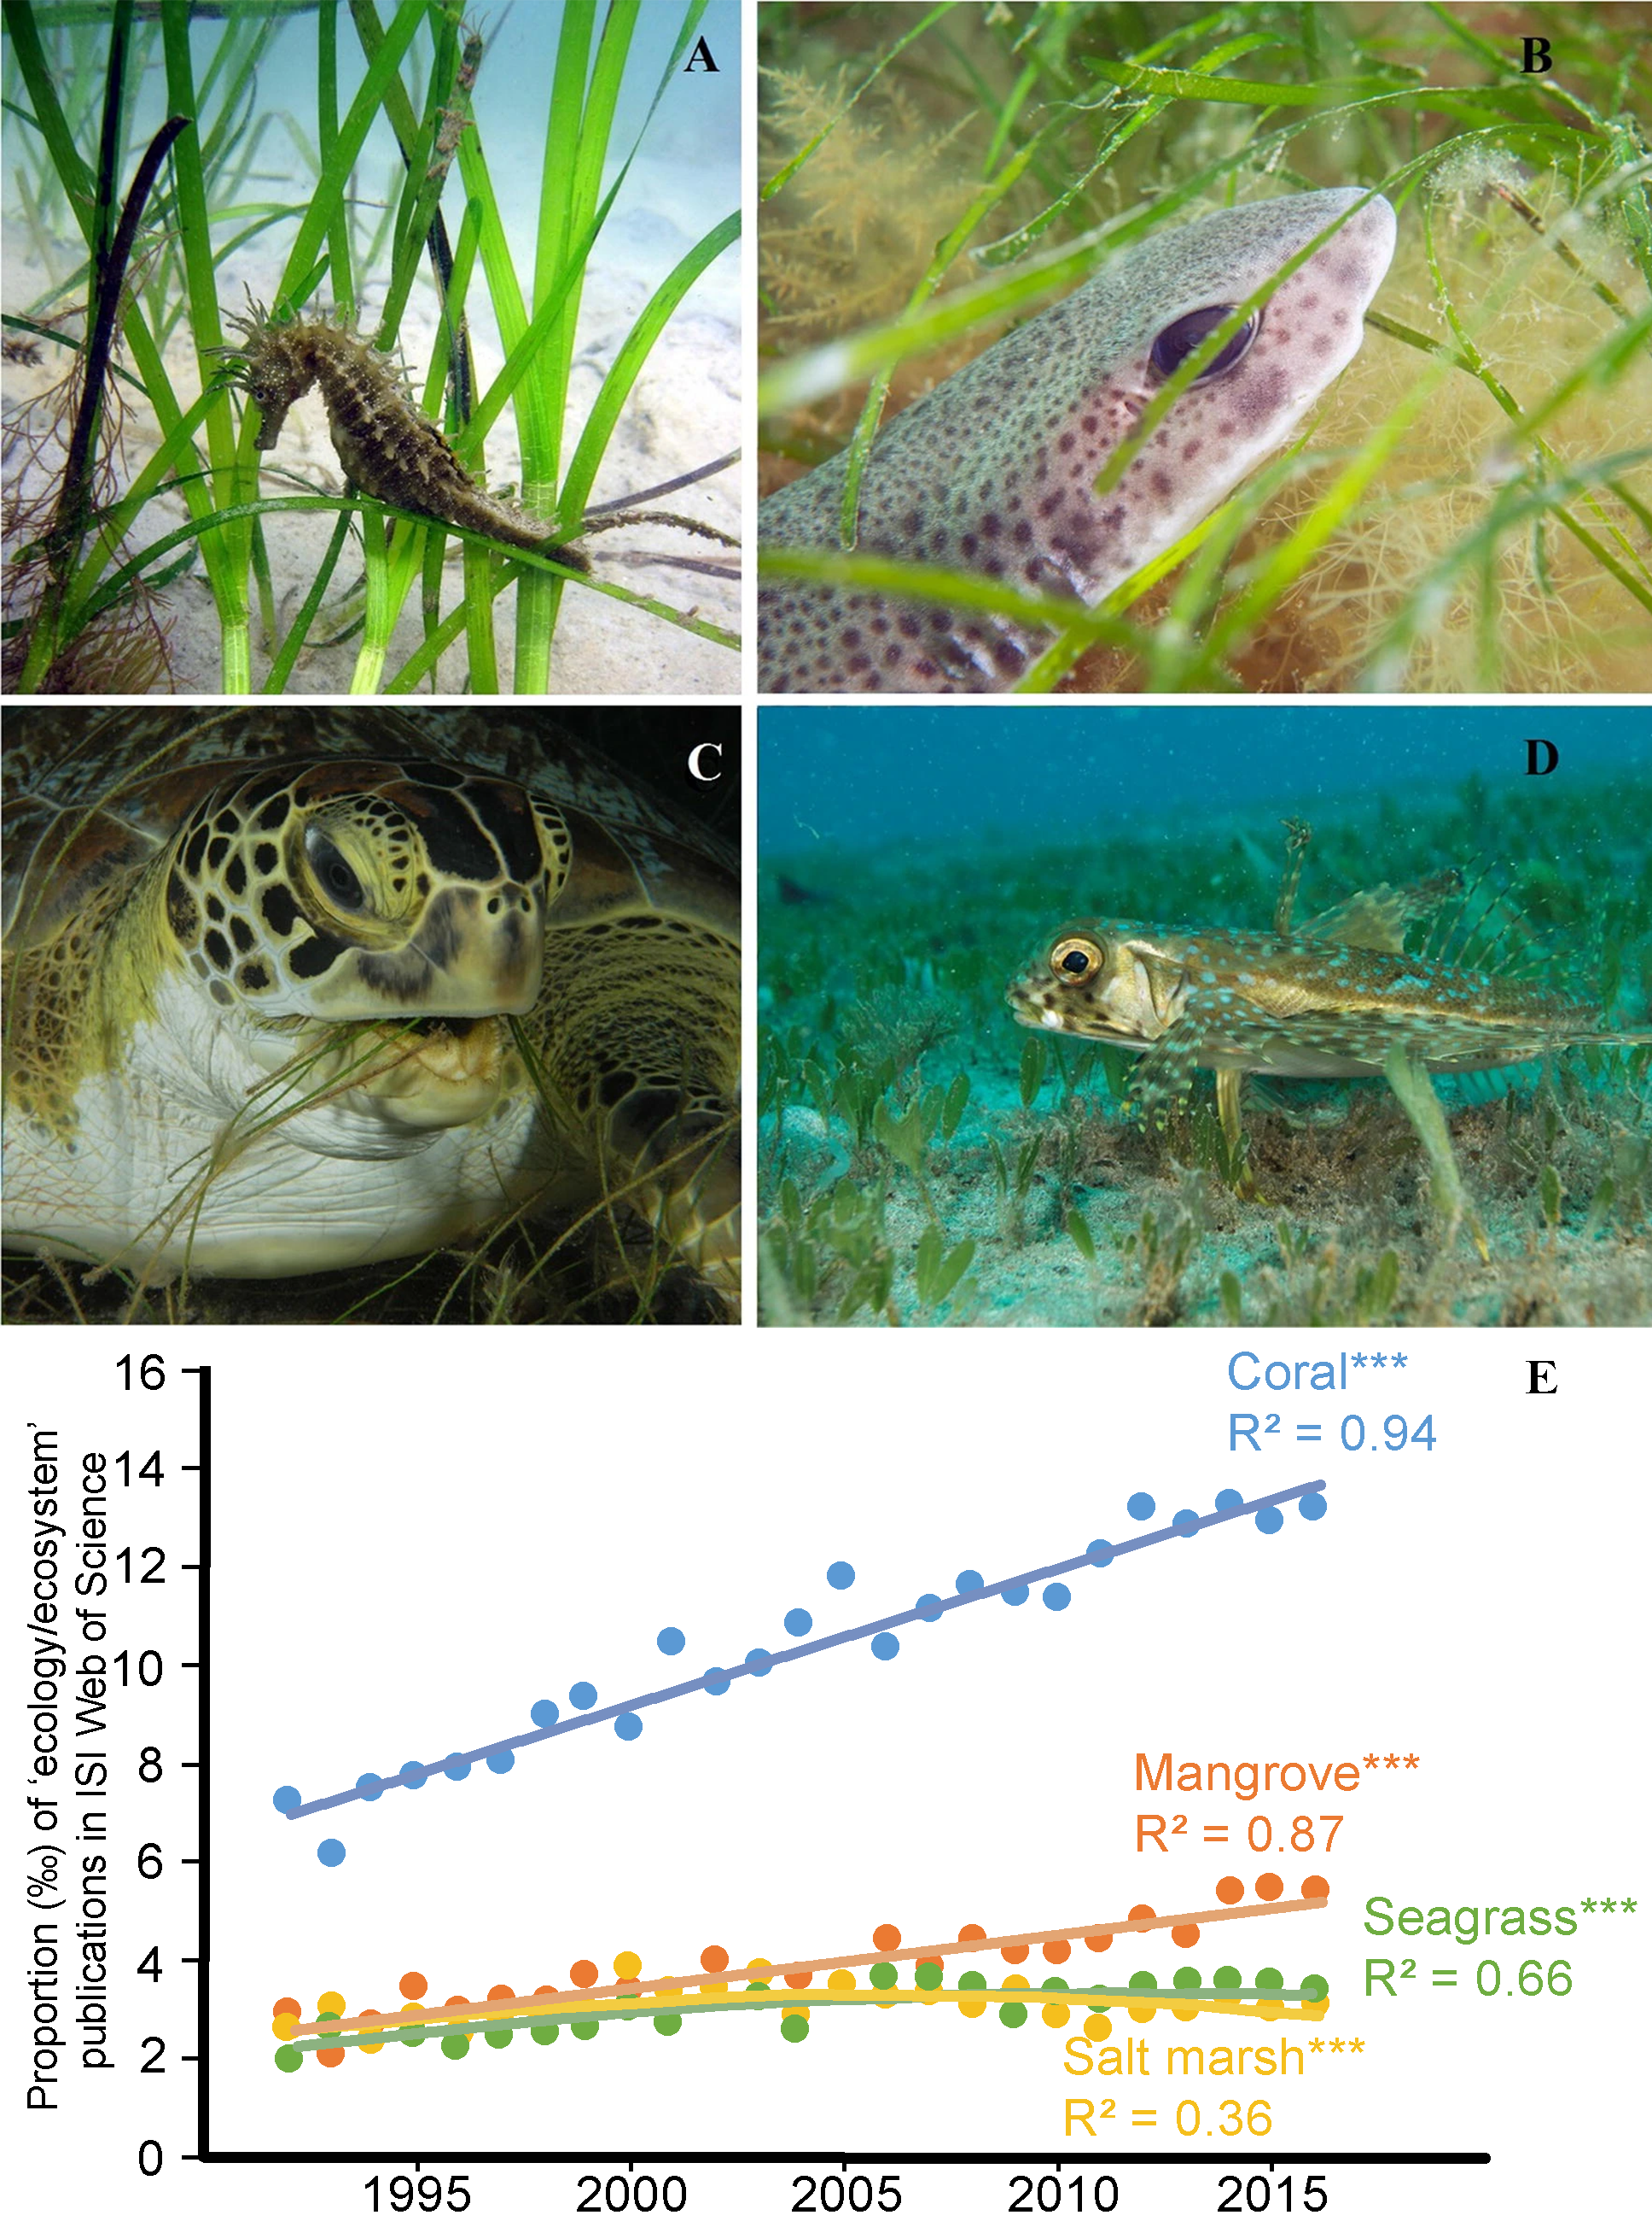
\includegraphics[width=1\linewidth,height=\textheight,keepaspectratio]{Chapter1/Figs/Publication_habitat/Seagrass_habitats.png}

}

\caption{\label{fig-SeagrassHabitat}Seagrass meadows are habitats
containing biodiverse faunal communities such as the following: a) the
Spiny Seahorse (\emph{Hippocampus guttulatus}) in the UK (source N
Garrick-Maidment), b) Dogfish (\emph{Scyliorhinus canicula}) in the UK
(source Frogfish Photography), c) the Green Sea Turtle (\emph{Chelonia
mydas}) in the Dutch Antilles, d) Flying Gurnard (\emph{Dactylopterus
volitans}) in Puerto Rico (source Luis R. Rodriguez) and e) shows the
proportion of publication each year dedicated to Coral reefs, Mangroves,
Seagrasses and Salt marshes. Modified from Unsworth et al. (2019a).}

\end{figure}%

Their structural complexity offers refuge from predators, supporting
juvenile survival and biodiversity. These meadows play a significant
role in global carbon sequestration, capturing and storing carbon at
rates comparable to, or exceeding, terrestrial forests. Furthermore,
they regulate nutrient cycles and improve water quality by trapping
sediments and filtering pollutants, thus sustaining the health of
adjacent marine environments (Los Santos et al., 2019). By cycling
nutrients and contributing organic matter through detritus production,
intertidal seagrass meadows enhance tidal flats' ecological productivity
and resilience, underscoring their critical role in supporting both
ecological functions and socio-economic benefits. Seagrass meadows, like
tidal flats, are undergoing significant dglobal decline due to various
anthropogenic and natural stressors (Davies et al., 2024a). Despite
their critical ecological roles, seagrass ecosystems remain
comparatively underrepresented in scientific research within the broader
scope of coastal ecosystems. As illustrated in
Figure~\ref{fig-SeagrassHabitat} (E), the proportion of publications
focusing on seagrasses in the context of coastal ecosystem studies is
considerably lower than those dedicated to other key habitats such as
coral reefs, mangroves. This disparity highlights a critical research
gap, underscoring the need for increased scientific attention to better
understand and mitigate the factors contributing to the degradation of
these vital ecosystems.

\newpage

\begin{tcolorbox}
Traditional field-based sampling methods have proven to be highly effective for studying coastal environments at localized or small spatial scales, providing detailed insights into species composition, habitat structure, and ecological interactions. However, these approaches face significant limitations when applied to broader spatial extents or temporal scales due to their labor-intensive nature and logistical constraints. This methodological gap poses challenges for evaluating large-scale patterns and long-term changes in coastal ecosystems, such as seagrass meadows, mangroves, and tidal flats. Remote sensing technologies, with their ability to capture high-resolution data across extensive geographic areas and over multiple time periods, offer a powerful complementary tool to address these limitations. Integrating traditional methods with remote sensing approaches allows a more comprehensive understanding of coastal ecosystem dynamics, facilitating the assessment of both localized impacts and global trends. However, spectral discrimination challenges arise when similar pigment compositions, such as those of seagrasses and green macroalgae, create overlapping spectral signatures in the visible and near-infrared regions. This issue is further compounded by vegetation mixing, where heterogeneous habitats result in mixed pixels that blend signals from multiple vegetation types and substrates. The following section explores how advancements in remote sensing technologies are transforming the study of coastal environments, enabling more efficient and scalable assessments.
\end{tcolorbox}

\section{Concepts of Remote sensing}\label{concepts-of-remote-sensing}

Coastal environments represent highly dynamic and sensitive ecosystems
shaped by complex interactions between natural processes and human
activities. Remote sensing (RS) technologies are crucial for monitoring
these regions, providing detailed data on shoreline erosion, habitat
degradation, sediment dynamics, and water quality. This section reviews
fundamental concepts and methodologies of RS applied to coastal
environments.

RS defines the ability to retrieve information in a non-invasive way,
without direct contact with the target. It relies on the propagation of
signals, typically optical, acoustic, or microwave, between the target
and the sensor. RS provides the basis for Earth observation (EO), where
its methodologies facilitate large-scale and long-term data collection.
Instruments on satellites, aircraft, and drones provide high-resolution
imagery and measurements critical for monitoring environmental changes,
mapping natural resources, and assessing land use patterns. These
technologies enable systematic data collection over large areas and
extended periods, supporting analyses such as deforestation, glacial
melting, variations in ocean temperature, and changes in land use.

\begin{tcolorbox}
Some technical characteristics of remote RS can directly impact their ability to map coastal ecosystems. The next section explores these characteristics, illustrating their importance with specific use case examples.
\end{tcolorbox}

\subsection{Active Remote Sensing, Example of
LiDAR}\label{active-remote-sensing-example-of-lidar}

Active RS is a technique in which a sensor emits its own
energy---typically in the form of electromagnetic radiation---toward a
target and measures the energy reflected or backscattered from it. This
method allows for the collection of data regardless of natural light
conditions, enabling observations during both day and night and through
various weather conditions.

The Light Detection and Ranging (LiDAR) sensor emit laser beams in the
ultraviolet (UV), visible or infrared (IR) regions of the
electromagnetic spectrum. By analyzing the return signal, they can
estimate distances to objects or surfaces, detect optically active
constituents in water bodies, and assess aerosols in the atmosphere
(Dionisi et al., 2024; Jamet et al., 2019)

LiDAR works by emitting a beam of light and measuring the time it takes
for the beam to return to the sensor. This process not only calculates
distances but also captures the intensity of the returned signal. In
many instances, multiple returns from a single pulse are measured,
enabling the mapping of varying objects height within the same x and y
coordinates. This capability allows the creation of precise,
three-dimensional representations of the environment such as mapping the
heights of trees in forests or measuring crop heights in agricultural
fields (Figure~\ref{fig-LIDAR}). When ground height cannot be directly
measured, LiDAR data can generate a digital surface model (DSM), which
represents the uppermost layer of the environment. However, if multiple
returns are recorded, it becomes possible to create both a DSM and a
digital terrain model (DTM), which represents the ground surface, by
differentiating between the surface and underlying layers. The
difference between DSM and DTM, called Digital Height Model (DHM), can
be used to assess living stock or biomass.

\begin{figure}

\centering{

\includegraphics[width=0.7\linewidth,height=\textheight,keepaspectratio]{Chapter1/Figs/LIDAR.png}

}

\caption{\label{fig-LIDAR}Diagram showing several signal-return for a
single emitted beam of a LIDAR system. adapted from Wang and Fang (2020)
and Garcı́a-Feced et al. (2011)}

\end{figure}%

Achieving accurate 3D measurements of a target using LiDAR technology
requires a high level of precision in assessing each system parameter.
The quality of the final output depends on careful calibration and
execution at every stage of the process. One critical step is ensuring
the precise timing of the laser beam's return after it reflects off the
target. This timing directly determines the distance calculations that
form the basis of the 3D structure. Equally important is the accurate
positioning of the LiDAR sensor, which is often mounted on a drone,
aircraft, or satellite. The sensor's x, y, and z coordinates must be
continuously tracked with high precision. Real-Time Kinematic (RTK)
positioning systems are commonly employed to achieve this. These systems
enhance the accuracy of the positioning data by providing real-time
corrections to the sensor's GPS coordinates, ensuring minimal error and
maintaining the integrity of the spatial measurements. Without such
stringent measures, the resulting LiDAR data is prone to errors that can
lead to distorted and noisy representations of the mapped surface. These
inaccuracies diminish the data's reliability and compromise its utility
for detailed analysis and decision-making processes.

In coastal environment monitoring, LiDAR systems are classified based on
their emitted wavelengths, which determine their performance and
application. These systems are categorized into ``topographic LiDAR''
and ``bathymetric LiDAR,'' each suited to specific tasks in coastal
studies. Topographic LiDAR operates in the near-infrared (NIR) spectrum
(approximately 1000 nm) and maps terrestrial features, such as beach
contours, vegetation density, rocky shore structures and man-made
installations. Its ability to generate high-density point clouds stems
from efficient operation at lower power. Unlike other types of LiDAR,
NIR LiDAR requires less power, making it generally more affordable and
compact. These attributes allow topographic LiDAR systems to be easily
mounted on drone platforms, offering greater flexibility and
accessibility for coastal monitoring. In contrast, bathymetric LiDAR,
utilizing green (\textasciitilde532 nm) and red wavelengths, penetrates
the water column to reveal submerged landscapes, including coral reefs,
seagrass meadows, and shallow seabeds. Operating within the visible
region of the electromagnetic spectrum, it is more susceptible to
atmospheric scattering than NIR LiDAR, making it less suitable for
terrestrial applications.

The Litto3D® product (SHOM, n.d.) consists of high-resolution
bathymetric and topographic maps in coastal areas created using LiDAR
technologies. During airborne missions, the system captures terrestrial
and submerged terrain features with high precision. The topographic
LiDAR achieves a spatial resolution of 1 m, with vertical accuracy up to
20 cm under optimal conditions, such as minimal atmospheric
interference, stable flight paths, and favorable weather. The
bathymetric LiDAR maps underwater landscapes to depths of approximately
70 m, depending on water transparency. This dual-mode capability is
essential for modeling complex coastal environments, seamlessly
integrating terrestrial and marine datasets. The airborne platform
enables rapid data acquisition over large areas, overcoming challenges
associated with ground-based or shipborne methods. The fusion
methodology used by Litto3D® ensures the precise alignment of
terrestrial and marine datasets, resolving inconsistencies in elevation
data at land-water interfaces. The resulting unified dataset accurately
represents coastal environments and supports diverse scientific and
practical applications such as coastal risk assessment and ecological
studies. Distributed by the Service Hydrographique et Océanographique de
la Marine (SHOM, 2024) and the Institut National de l'Information
Géographique et Forestiere (IGN, 2024a), this dataset is open-source but
currently available only for selected coastal regions in France.

In this study, LiDAR data were utilized in \textbf{Chapter 4} using a
drone-borne NIR LiDAR system. These data were employed to evaluate the
elevation and slope of mudflats in French and Spanish estuaries and to
map the spatial distribution of the invasive red macroalga
\emph{Gracilaria vermiculophylla}. In \textbf{Chapter 5}, the Litto3D
product was and a water height dataset were used to assess the emersion
time of seagrass meadows in Quiberon, France, during low tide. Since
this thesis focuses on intertidal environment, field campaigns were
conducted during low tide to ensure optimal conditions for the effective
use of NIR LiDAR providing unobstructed access to exposed intertidal
zones.

\subsection{Passive Remote Sensing}\label{passive-remote-sensing}

Passive RS collects data about the Earth's surface or atmosphere by
measuring naturally emitted or sunlight-reflected electromagnetic
radiation (EMR) without actively transmitting signals. This technique
relies on energy sources external to the instrument, such as sunlight
for optical and NIR sensors or Earth's thermal emissions for thermal
infrared sensors.

Passive RS is widely utilized in spaceborne satellite missions and has
played a pivotal role in programs developed by major space agencies,
including the European Space Agency (ESA) and the National Aeronautics
and Space Administration (NASA). For instance, Sentinel-2 which provides
ESA's highest spatial resolution imagery, employs passive sensors. Data
measured by these sensors have been applied to monitor land cover,
vegetation dynamics and coastal and in land-water environments.

As sunlight enters the Earth's atmosphere, it interacts with various
gases and particles altering its properties. These interactions include
scattering, absorption, and refraction. Scattering occurs when
atmospheric molecules and aerosols disperse light in different
directions, with shorter wavelengths like blue light being more strongly
affected. Absorption results from atmospheric constituents such as
ozone, water vapor, and carbon dioxide, which absorb energy at specific
wavelengths, reducing the intensity of the transmitted light that
reaches the Earth's surface. Refraction occurs as light changes
direction and speed while passing through atmosphere layers with varying
densities (Figure~\ref{fig-FigLightPath}).

When sunlight reaches the Earth's surface, it exhibits several
behaviors, depending on the surface properties and the angle of
incidence. These behaviors include:

\begin{itemize}
\item
  Absorption: The surface absorbs light, converting it into heat or
  another form of energy. This process varies based on the
  biogeochemical characteristics of the surface, with darker surfaces
  typically absorbing more light.
\item
  Transmission: The light passes through the surface, entering a
  different medium, such as water or transparent materials. The extent
  of transmission depends on the material's transparency and refractive
  index.
\item
  Reflection: Light that is neither absorbed nor transmitted is
  redirected back in the opposite direction. The amount of reflection
  depends on the surface's albedo, with bright surfaces like snow
  reflecting more light compared to darker surfaces such as forests.
\end{itemize}

Only reflected light can be detected by spaceborne sensors. The most
used metric in passive RS, to quantify EMR, is reflectance (\(R\)).
\(R\) is typically measured as the ratio of upwelling radiance \(L_u\)
to downwelling radiance \(L_d\) (Equation~\ref{eq-reflectance}). \(L\)
is defined as the radiant intensity per unit of projected area in a
specified direction and is expressed in units of
W.m\textsuperscript{-2}.sr\textsuperscript{-1}. \(R\), however, is
dimensionless.

\begin{equation}\phantomsection\label{eq-reflectance}{
R(\lambda) = \frac{L_u(\lambda)}{L_d(\lambda)}
}\end{equation}

\(R\) is defined for each wavelength as a value between 0 and 1. A value
of 0 indicates that all light has been absorbed or transmitted by the
target, while a value of 1 indicates that all light has been reflected
(Figure~\ref{fig-FigLightPath}).

\begin{figure}

\centering{

\includegraphics[width=0.9\linewidth,height=\textheight,keepaspectratio]{Chapter1/Figs/FigLightPath.png}

}

\caption{\label{fig-FigLightPath}Light pathways involved in remote
sensing: illustrating the interaction of solar radiation with the
atmosphere, vegetation, and water surfaces, highlighting processes such
as scattering, absorption, and reflectance contributing to the
top-of-atmosphere (TOA) radiance observed by a satellite sensor.}

\end{figure}%

\(R\) at the Top of Atmosphere (TOA), i.e., the magnitude directly
measured by spaceborne or airborne sensors contains signals originating
from both the atmosphere and the Earth's surface. Therefore, to study
targets located on the Earth's surface, \(R_{TOA}\) must undergo
atmospheric correction processing to transform it into Bottom of
Atmosphere (BOA) \(R\), which represents the intrinsic reflectance
properties of the surface target. Precise \(R_{BOA}\) is crucial for
accurately analyzing surface characteristics and for applications like
vegetation monitoring, water quality assessment, and land cover
classification.

One of the most basic atmospheric correction methods is the ``black
pixel'' method, which assumes that all the signal retrieved over
optically deep waters originates entirely from the atmosphere. This
information is then used to correct the reflectance across the entire
scene. However, this method requires the presence of optically deep
water targets within the scene and assumes uniform aerosol
concentrations across the scene. Such assumption may be inaccurate,
particularly for satellites with a wide field of view, such as MODIS,
where a single image can cover a swath of 2,330 km. Limitations to this
technique also arise when the target of study is a water body itself.
These limitations highlight the need for more advanced correction
techniques that account for spatial variability in atmospheric
properties.

To address these challenges, sophisticated atmospheric correction
algorithms tailored to specific sensors and study areas have been
developed. These algorithms account for atmospheric scattering,
absorption, and path radiance contributions by leveraging radiative
transfer models, auxiliary atmospheric data, and sometimes \emph{in
situ} measurements. For example, data from the ESA constellation
Sentinel-2 can be processed using Sen2Cor, a correction algorithm
designed to produce \(R_{BOA}\) by incorporating atmospheric parameters
such as water vapor, aerosols, and ozone concentrations. Additionally,
some atmospheric correction methods are customized for specific targets,
for example, algorithms specifically designed for water bodies, such as
POLYMER (Steinmetz et al., 2011) or ACOLITE (Vanhellemont and Ruddick,
2018).

\(R_{BOA}\) provides information regarding light reflected by the target
across various wavelengths. This phenomenon, referred to as the spectral
signature, is a unique feature of each target type. Spectral signatures
contain data about the physical and chemical properties of surfaces,
forming the basis for RS applications. By analyzing spectral signatures,
it is possible to identify and classify surface types, as well as derive
insights into environmental changes and land-use dynamics. For example,
Chlorophyll-a (Chla), a pigment found in all vegetation cells, plays a
key role in defining the spectral signature of plant life. Chla absorbs
light in specific regions of the electromagnetic spectrum, particularly
in the blue region around 440 nm and the red region near 675 nm.
Consequently, healthy vegetation exhibits a spectral signature with low
\(R\) at 440 and 675 nm. Variations in physiological states and
vegetation types result in different spectral patterns, enabling their
differentiation and monitoring of ecological conditions over time
(Figure~\ref{fig-Spectral_signature}).

\begin{figure}

\centering{

\includegraphics[width=0.8\linewidth,height=\textheight,keepaspectratio]{Chapter1/Figs/spectral_signatures.png}

}

\caption{\label{fig-Spectral_signature}The spectral signature of
vegetation (green), Water (blue) and bare soil (red). Absorption
features of Chlorophyll-a are indicated for the spectra of vegetation.}

\end{figure}%

Spectral indices are mathematical combinations of reflectance values at
specific wavelengths, designed to maximize particular surface
characteristics with simple processing. Vegetation indices, for example,
leverage the distinct reflectance patterns of photosynthetic pigments.
The Normalized Difference Vegetation Index (NDVI) is a widely used index
based on the normalized difference between \(R\) in the NIR and red. It
is calculated as:

\begin{equation}\phantomsection\label{eq-NDVI}{
NDVI = \frac{R(NIR)-R(Red)}{R(NIR)+R(Red)}
}\end{equation}

where \(R(NIR)\) is the reflectance in the NIR region around 800 nm and
\(R(Red)\) is the reflectance in the red region arround 665 nm.

NDVI values range from -1 to 1, with negative values indicating water
and higher positive values corresponding to dense healthy vegetation.
While NDVI is a proxy for vegetation biomass and photosynthetic
activity, its interpretation can be complex in heterogeneous
environments, such as areas with overlapping vegetation types or
substrates. Some studies propose a simple classification of NDVI based
on thresholds to differentiate between distinct types of intertidal
vegetation (Méléder et al., 2003b). While this simple first
approximation can be useful for delimitating contrasting types of
targets, establishing thresholds depends on specific sensor
characteristics. This technique often fails in mapping vegetation types
with similar pigment content or highly heterogeneous targets. More
sophisticated techniques that utilize a greater amount of spectral
information are required in such situations (Oiry and Barillé, 2021)

\(R_{BOA}\) can be used to identify key absorption features of chemical
compounds of the target, by applying derivative analysis to the spectral
signature. The second derivative of the \(R\) is utilized to enhance the
detection of subtle pigment or mineral absorption features. By analyzing
the second derivative, these small features are amplified, allowing for
more precise identification of pigment presence and estimation of their
concentrations. This approach is particularly effective for identifying
accessory pigments with weaker absorption features than Chla (Jesus et
al., 2014).

\begin{tcolorbox}
Some technical characteristics of RS sensors can directly impact their ability to map coastal ecosystems. The next section explores these characteristics, illustrating their importance with examples of specific use cases.
\end{tcolorbox}

\subsubsection{Spectral and Radiometric
resolution}\label{spectral-and-radiometric-resolution}

The detection of pigments absorption features necessitates measuring
light reflectance at fine spectral resolution. However, measuring
detailed spectral signatures depends on the sensor's characteristics.

Spectral resolution is defined by three main components: the number of
spectral bands, the bandwidth (Full Width at Half Maximum, FWHM), and
the spectral sampling interval. Sensors with higher spectral resolution
can distinguish between closely spaced wavelengths within the
electromagnetic spectrum, enabling precise characterization of spectral
features (Figure~\ref{fig-Spectral_resolutions}).

\begin{figure}

\centering{

\includegraphics[width=1\linewidth,height=\textheight,keepaspectratio]{Chapter1/Figs/Spectra_resolutions/Fig_SpectralResolution_chouchou.png}

}

\caption{\label{fig-Spectral_resolutions}Comparison of spectral
resolution between multispectral (A) and hyperspectral (B) sensors in
the solar radiance spectrum. Panel C illustrates the impact of spectral
resolution on the same spectral signature of \emph{Gracilaria
vermiculophylla}. With hyperspectral resolution (red), absorption
features of pigments such as phycocyanin and phycoerythrin are
distinguishable, whereas these features are absent in the multispectral
resolution provided by Sentinel-2 (green). D is showing examples of
different radiometric resolutions for the same band of a Sentinel-2
tile. One is coded in 12 bits (left), and the other in 6 bits (right).}

\end{figure}%

RS sensors are generally classified into two categories based on their
spectral resolution: multispectral and hyperspectral sensors.
Multispectral sensors are characterized by a limited number of broad
spectral bands, with a bandwidth generally exceeding 20 nm. The spectral
sampling interval is relatively large, resulting in a coarser spectral
resolution that provides a broad overview of the spectral
characteristics of a scene. In contrast, hyperspectral sensors are
equipped with hundreds of narrow, contiguous spectral bands. Small
spectral sampling intervals separate these bands, often just a few
nanometers, which results in a much finer spectral detail. High spectral
resolutions, capturing subtle variations in absorption features and
spectral shapes, allow distinguishing between targets with similar
spectral characteristics, such as vegetation with similar pigment
profile. Multispectral sensors, while less detailed, are efficient for
general spectral analyses where fine discrimination is not required.
Another specification of sensors in the spectral discrimination is the
radiometric resolution. It refers to the precision at which the sensor
records the data. It is defined by the number of discrete levels, or
bits, used to represent the energy recorded for each pixel in an image.
Higher radiometric resolution enables finer distinctions in brightness
levels, which is particularly important for detecting subtle differences
in reflectance and ensuring accurate analysis of surface features. For
example, an 8-bit sensor can record 256 levels of intensity, while a
12-bit sensor can capture 4,096 levels, providing greater detail and
dynamic range in the captured imagery
(Figure~\ref{fig-Spectral_resolutions} D).

\subsubsection{Spatial resolution}\label{spatial-resolution}

Spatial resolution, defined as the smallest discernible detail a sensor
can detect on Earth's surface, is another fundamental characteristic of
RS sensors. It is typically represented by the ground area covered by a
single pixel in an image and is influenced by the sensor's instantaneous
field of view (IFOV), which determines the angle of view and,
consequently, the ground area visible to the sensor. A smaller IFOV or
lower sensor altitude results in finer spatial resolution, enabling the
detection of smaller features. For the same IFOV, sensors mounted on
satellites can cover larger areas compared to those on drones, albeit
with reduced detail.

Spatial resolution can range widely depending on the research objective
and sensor platform. For instance, moderate-resolution sensors like
MODIS aboard Terra and Aqua capture data at spatial resolutions of 250
m, 500 m, and 1 km, making them suitable for large-scale environmental
monitoring. In contrast, Sentinel-2 provides higher spatial
resolutions---10 m for visible and NIR bands, 20 m for red-edge and
shortwave infrared bands, and 60 m for atmospheric correction
bands---facilitating detailed observations for applications such as
vegetation and land-use mapping. At the finer end, high-resolution
sensors on platforms like Pleiades-Neo achieve sub-meter resolutions
(e.g., 30 cm per pixel), ideal for precise Earth observations.

Unmanned Aerial Vehicles (UAVs), equipped with high-resolution cameras,
offer even finer spatial resolutions, often down to a few cm, even mm,
depending on flight altitude and sensor specifications. This ultra-high
resolution is particularly advantageous for heterogeneous site mapping.
Chapter 3 will show that an ultra-high spatial resolution can be
valuable for machine learning model training. However, such a high
resolution requires increased data storage and processing capacity,
illustrating the trade-off between detail and operational feasibility
(Section~\ref{sec-Drones}).

In scenarios involving mixed vegetation types or intricated landscape
features, coarse-resolution sensors may fail to capture fine-scale
heterogeneity, limiting the accuracy of ecological or land-use analyses.
Conversely, high-resolution imagery excels in such contexts but demands
significant computational resources. Selecting the appropriate spatial
resolution depends on specific research objectives and the spatial scale
of the phenomena under investigation, underscoring the necessity of
aligning sensor capabilities with study requirements.

\subsubsection{Temporal Resolutions}\label{temporal-resolutions}

Another key characteristic of RS sensors is their temporal resolution,
defined as the time interval between successive image acquisitions over
the same study site. Temporal resolution is critical for monitoring
dynamic environments, such as coastal ecosystems, where conditions can
change rapidly due to tides, weather events, or human activity.

The temporal resolution of a satellite sensor may vary from hours to
days, depending on whether the platform orbit is geostationary or
sun-synchronous. Geostationary satellites provide continuous coverage
over a fixed location, while sun-synchronous orbits follow sun
illumination, allowing image acquisition at the same time of the day for
a location. This consistency is particularly important for
visible-infrared sensors, as it ensures usable images and maximizes the
temporal resolution of the sensor by avoiding night-time acquisitions.
On the other hand, airborne platforms exhibit more variable temporal
resolutions, ranging from days to years, depending on mission planning.
For example, the Sentinel-2 constellation, composed of two satellites,
offers a temporal resolution of 5 days at the equator. This revisit time
improves to approximately 3 days at higher latitudes, such as in France,
due to the overlap in satellite paths. Such frequent revisits make
Sentinel-2 an excellent choice for applications requiring consistent
monitoring, such as vegetation health assessments, sediment transport
studies, or vegetation phenology estimations. Certain missions, like
Sentinel-3, achieve even shorter revisit times. Equipped with sensors
designed for ocean and land monitoring, Sentinel-3 provides near-daily
coverage, making it particularly suited for applications that require
high temporal frequency, such as tracking phytoplankton blooms, which
can appear and disappear within a few days, or surface temperature
variations. This capability is crucial for capturing fast-evolving
phenomena and ensuring timely data delivery for decision-making.

Usually, temporal resolution is highly dependent on the spatial
resolution of the sensor. Higher spatial resolution often corresponds to
lower temporal resolution, although geostationary platforms and
pointable sensors can be exceptions to this trend
(Figure~\ref{fig-ResolutionSatellite}).

In contrast, some sensors are operated on-demand, with data acquisition
triggered directly by the user. This is characteristic of drones and
specialized satellite missions like Pleiades or the italien Precursore
IperSpecttrale della Missione Applicativa (PRISMA). While these systems
may lack consistent temporal archives for a given study site, they
provide unmatched flexibility for high-resolution data collection. Such
sensors are invaluable for addressing specific research objectives,
including acquiring detailed imagery immediately after extreme weather
events or capturing localized features with high spatial precision,
complementing routine satellite-based monitoring programs.

\subsubsection{A story of trade-off}\label{a-story-of-trade-off}

RS involves inherent trade-offs between spatial, temporal and spectral
resolutions, and coverage area, which influence the suitability of
sensors for different applications
(Figure~\ref{fig-ResolutionSatellite}). High spatial resolution sensors,
capable of capturing fine-scale details, are essential for precise tasks
like urban infrastructure mapping or site-specific ecological studies.
In coastal environments, high-resolution sensors are invaluable for
identifying small-scale features such as intertidal vegetation patterns,
sediment deposition dynamics. However, these sensors typically have
lower temporal resolution and smaller coverage areas, limiting their
utility for monitoring dynamic or widespread phenomena, such as tracking
algal bloom events across entire coastal regions.

\begin{figure}

\centering{

\includegraphics[width=1\linewidth,height=\textheight,keepaspectratio]{Chapter1/Figs/Satellite_resolution.png}

}

\caption{\label{fig-ResolutionSatellite}Intersection of spectral
resolutions (x-axis), temporal resolutions (y-axis), and spatial
resolutions (circle size) of the main satellite sensors used to observe
coastal areas.}

\end{figure}%

In contrast, sensors with coarser spatial resolution offer extensive
coverage and higher revisit frequencies, making them ideal for tracking
large-scale environmental changes. For coastal areas, these sensors can
effectively monitor phenomena such as Sea Surface Temperature (SST)
variability, coastal erosion trends, and seasonal changes in primary
productivity over larger geographic extents. For example, instruments
like MODIS or VIIRS are well-suited for observing ocean color and Chla
concentrations, critical for understanding broader ecosystem health in
coastal zones.

Intermediate-resolution sensors provide a compromise, offering
sufficient spatial detail for regional studies while maintaining
adequate temporal resolution for periodic monitoring. These are
particularly useful for applications such as mapping coastal vegetation
transitions, estuarine dynamics, and changes in sediment plumes from
rivers into the ocean over time. Instruments like Sentinel-2 or Landsat
provide this balance, making them key assets for monitoring coastal
ecosystems at scales relevant to regional management.

The selection of an appropriate sensor depends on the specific
requirements of the study, balancing the need for detail, frequency, and
geographic extent. Coastal zone management, for instance, often benefits
from using a combination of sensors to capture both fine-scale spatial
patterns and broader temporal trends, ensuring comprehensive monitoring
of these dynamic environments.

While satellite acquisitions are essential for covering large areas,
heterogeneous habitats often require finer spatial resolutions,
positioning drones as the most suitable observation tool. Drone-based
studies can also serve as proof-of-concept techniques to refine and
develop methodologies later applicable to satellite data.

\begin{tcolorbox}
Although this work builds upon many of the concepts introduced in the previous sections, one critical RS technique warrants further discussion in this introduction. This technique, characterized by its adaptability and technical precision, provides essential insights and complements the methods already outlined. The next section will introduce drones, focusing on their application as a RS tool and detailing the associated techniques and data analysis methods.
\end{tcolorbox}

\subsection{About Drones}\label{about-drones}

\subsubsection{History}\label{history}

At the beginning of the 20\textsuperscript{th} century, Julius
Neubronner, a German apothecary, faced a logistical challenge in his
professional practice. Neubronner regularly relied on carrier pigeons to
deliver and retrieve small, urgent medical packages, such as medications
or prescriptions, between his pharmacy and a sanatorium located several
kilometers away. This method, though efficient for short distances,
often left Neubronner curious about the exact routes taken by the
pigeons and the environmental conditions they encountered during their
flights. Motivated by both practical concerns and a spirit of
innovation, Neubronner sought a way to monitor and document the journeys
of his pigeons. He developed a lightweight, auto-triggering camera that
could be strapped to the pigeons' chests (Figure~\ref{fig-pigeons} Top).
The camera was designed to automatically take photographs at regular
intervals during the birds' flights. It had two lenses and a pneumatic
system; it was activated by inflating the left chamber. As the air
slowly escaped from the capillary at the bottom, the piston moved back
triggering the exposure. Neubronner ensured that the camera was light
enough not to impede the pigeons' ability to fly (Simic Milas et al.,
2018).

\begin{figure}

\centering{

\includegraphics[width=0.9\linewidth,height=\textheight,keepaspectratio]{Chapter1/Figs/Neubronners/pigeons_compositions.png}

}

\caption{\label{fig-pigeons}One of Neubronner's pigeons (Top), around
1910 equipped with a camera. The bottom shows a picture taken during a
pigeon's flight.}

\end{figure}%

The resulting aerial photographs offered a novel perspective, capturing
bird's-eye views of landscapes, towns, and natural features
(Figure~\ref{fig-pigeons} Bottom). These images not only satisfied
Neubronner's initial curiosity about the pigeons' routes but also
demonstrated the broader potential of aerial photography for
cartography, reconnaissance, and environmental observation. His
innovative work garnered widespread attention, paving the way for
further developments in RS and aerial imaging. Neubronner's experiments
illustrated the practical applications of aerial imaging at a time when
such perspectives were almost entirely unavailable, highlighting his
contributions to science and art.

Julius Neubronner's early vision exemplifies how innovative thinking can
overcome barriers in data collection. For many years, the practical
limitations of RS technologies, particularly regarding spatial and
temporal resolution or the high costs and delays in data acquisition,
constrained their applicability in various fields. However, innovations
like drones have significantly addressed these challenges. Much like
Neubronner's pigeons, modern drones are not only accessible and
affordable but also offer users the freedom to determine when and where
to deploy them, providing unparalleled control over spatial and temporal
data collection. Neubronner's ingenuity in developing lightweight aerial
cameras for pigeons paved the way for these advancements, demonstrating
the enduring impact of pioneering solutions in expanding the potential
applications of RS.

Modern drone history has its roots in military applications, where the
need for unmanned surveillance and targeted operations drove the initial
technological advancements. Early drone systems, such as the use of
radio-controlled aircraft in World War II, laid the foundation for what
would become an essential tool in both civilian and military contexts.
The transition to civilian applications gained momentum in the late
20\textsuperscript{th} century, particularly with the advent of
lightweight materials, improved battery technologies, and advances in
GPS and RS capabilities. Today, drones are integral to various
industries, from precision agriculture and infrastructure inspection to
environmental monitoring and emergency response. This evolution reflects
the growing accessibility and versatility of drone technology, making it
a transformative element in modern data acquisition and analysis.

\subsubsection{General presentation}\label{sec-Drones}

Drones, also known as Unmanned Aerial Vehicles (UAVs), are aircraft
systems operated without a human pilot onboard. They are often embedded
with GPS and can be remotely controlled or fly autonomously through
software-controlled flight plans. These devices have become
indispensable tools in modern RS, offering high accuracy, on-demand data
acquisition, and access to previously unreachable locations. The growing
use of drones in various fields, from environmental monitoring to urban
planning, underscores their versatility and importance.

While drones are not inherently functional on their own, they become
highly effective tools when integrated with various sensors. These
include hyperspectral sensors (Suomalainen et al., 2021), multispectral
sensors (Nurdin et al., 2023; A. Román et al., 2023), RGB cameras (Sweet
et al., 2022), thermal cameras (Speth et al., 2022), LiDAR systems
(Krček et al., 2020; Lee et al., 2023), as well as gas and chemical
sensors.

\subsubsection{Data acquisition}\label{data-acquisition}

\begin{figure}

\centering{

\includegraphics[width=0.9\linewidth,height=\textheight,keepaspectratio]{Chapter1/Figs/Drone_overlaps.jpg}

}

\caption{\label{fig-overlaps}Schematic representation of image
overlapping of a drone}

\end{figure}%

A key parameter in drone-based image acquisition is the overlap between
images (Figure~\ref{fig-overlaps}). This is categorized as front overlap
(FO), which refers to the overlap between consecutive images along the
same flight path, and side overlap (SO), which pertains to the overlap
between images from adjacent flight paths. Ensuring sufficient overlap
is essential for accurate reconstruction of orthomosaics through
photogrammetric processes. Typically, 80\% front overlap and 70\% side
overlap are considered optimal to achieve reliable results. The
mathematical definitions of FO and SO are as follows:

\[
\text{FO} \;=\;
\left(1 - \frac{v \times \Delta t}{
  \frac{H \times h_{\text{sensor}}}{f}
}\right) \times 100
\]

\[
\text{SO} \;=\;
\left(1 - \frac{d_{\text{flight\_line}}}{
  \frac{H \times w_{\text{sensor}}}{f}
}\right) \times 100
\]

\subsection*{Where: }
\begin{itemize}
  \item $\text{FO}$: Forward Overlap (in \%)
  \item $\text{SO}$: Side Overlap (in \%)
  \item $v$: Ground speed of the drone (m/s)
  \item $\Delta t$: Time interval between consecutive photos (s)
  \item $H$: Flight altitude above the ground (m)
  \item $h_{\text{sensor}}$: Sensor height in the flight direction (mm)
  \item $w_{\text{sensor}}$: Sensor width perpendicular to the flight direction (mm)
  \item $f$: Camera focal length (mm)
  \item $d_{\text{flight\_line}}$: Distance between adjacent flight lines (m)
\end{itemize}

These equations show that for a given sensor (e.g., for known \(f\),
\(h_{\text{sensor}}\), \(w_{\text{sensor}}\), and \(\Delta t\)), the
only parameters that can be adjusted to ensure sufficient overlap are
the flight speed or the altitude of flights. If the user chooses to set
\(H\) (directly linked to the spatial resolution of the final product),
then \(v\) will be automatically fixed by the system. The higher the
flight altitude, the higher the flight speed, or conversely, if the user
chooses to set \(v\) (directly linked to the total time of the mission),
then the altitude will be locked by the system, resulting in a higher
\(v\) corresponding to a higher flight height.

The area that a drone can cover during a mission grows exponentially as
the flight height increases. However, while the maximum flight height
drones can technically reach is not inherently limited, it is strictly
regulated by law. In Europe, for instance, the maximum permitted flight
height is 120 m. This restriction can be a limiting factor for certain
applications, particularly when the area to be covered exceeds several
square kilometers. For instance, the largest intertidal seagrass meadow
in France is located in the Bassin d'Arcachon and covers an area of
nearly 40 km² (Cognat et al., 2018). Using a Micasense RedEdge-MX DUAL
multispectral sensor mounted on a drone flying at 120 m altitude at 10
m.s⁻¹, this area would take approximately 44 hours of flight time to
cover entirely. The total time required to map this entire area at low
tide could be further extended when accounting for constraints such as
daylight hours, tide cycles, battery recharging, potential
weather-related delays, and the need for the operator to frequently
reposition themselves due to regulatory restrictions that limit the
drone's distance to 1 km from the drone pilot.

\subsubsection{Data processing}\label{data-processing}

Satellite products produced by space agencies are often provided to
users after extensive preprocessing steps, including orthorectification,
precise georeferencing, radiometric calibration. Similarly, these
preprocessing steps are crucial for utilizing drone-acquired data
effectively. Nowadays, user-friendly software, such as Agisoft Metashape
and Pix4D, enables users to perform these essential steps efficiently,
making advanced data processing accessible even to non-expert users.
Steps to obtain an orthoimage from a bunch of single images will be
described now in more details.

\paragraph{Image pre-processing}\label{image-pre-processing}

The first step is to correct each individual image acquired by the drone
from optical distortion that occurred during its acquisition
(Figure~\ref{fig-img_preprocessing}). Photogrammetric software typically
addresses lens distortion and vignetting through a combination of camera
calibration and radiometric adjustments.

\begin{figure}

\centering{

\includegraphics[width=0.9\linewidth,height=\textheight,keepaspectratio]{Chapter1/Figs/distortion.png}

}

\caption{\label{fig-img_preprocessing}Schematic representation of image
pre-processing for orthomosaic reconstruction, showing correction of the
distortion (A \& B) and correction of the vignetting (C \& D).}

\end{figure}%

During calibration, the software refines intrinsic parameters such as
focal length, principal point offsets, and radial/tangential distortion
coefficients (called k1, k2, k3, p1, p2) by matching features across
overlapping images in a bundle adjustment process. Some camera
manufacturers provide sensor-specific metadata, including correction
factors, which can further enhance calibration accuracy. Vignetting,
which manifests as reduced brightness near the image edges, is often
corrected via additional vignetting coefficients or automated
radiometric calibration routines that normalize illumination across
photos. These corrections are essential for ensuring both geometric
precision in the 3D reconstruction and radiometric consistency in the
final orthomosaic.

\paragraph{Initial Image Alignment / Aerial
Triangulation}\label{initial-image-alignment-aerial-triangulation}

Once corrected, each image can be aligned. During the initial image
alignment phase, the photogrammetry software relies on Structure from
Motion (SfM) algorithms to identify unique tie points in overlapping
images and triangulate their 3D positions. These tie points are then
matched across the dataset, and a bundle adjustment is performed to
optimize camera parameters (position, orientation, and intrinsic
calibration). Often referred to as aerial triangulation, this step
produces a sparse point cloud that underpins all subsequent stages. Its
accuracy is critical, as it defines the precision of the final 2D and 3D
outputs.

\paragraph{Dense Point Cloud Generation}\label{sec-DPC}

Building upon the camera geometry established by SfM, the software uses
Multi-View Stereo (MVS) techniques to compute dense depth maps for each
overlapping image pair. These depth maps are merged to create a dense
point cloud containing millions---or even billions---of points,
capturing high-resolution details of the scene's geometry. Although
computationally intensive, this phase lays the groundwork for generating
accurate surface models and textured 3D representations later in the
workflow.

\paragraph{Digital Surface Model (DSM) / Digital Terrain Model
(DTM)}\label{digital-surface-model-dsm-digital-terrain-model-dtm}

From the dense point cloud, a DSM is derived by capturing the highest
elevation values within each pixel or grid cell, thereby representing
above-ground features like buildings and vegetation. Alternatively, a
DTM can be produced by classifying and removing non-ground points to
approximate the bare-earth surface. Both models are typically exported
as raster files and used in various analytical applications, such as
hydrological modeling, viewshed analysis, and volume calculations. Their
accuracy depends on the quality of the dense cloud and effective point
classification techniques. The difference between the DSM and the DTM is
called a Digital Height Model (DHM, Figure~\ref{fig-DSMDTM}).

\begin{figure}

\centering{

\includegraphics[width=0.9\linewidth,height=\textheight,keepaspectratio]{Chapter1/Figs/DSM_DTM.png}

}

\caption{\label{fig-DSMDTM}Representation of differences between the
Digital Surface Model (DSM), the Digital Terrain model (DTM) and the
Digital Height Model (DHM).}

\end{figure}%

\paragraph{Orthorectification and Orthomosaic
Creation}\label{orthorectification-and-orthomosaic-creation}

During orthorectification, the software projects each image onto the DSM
or DTM to correct for camera tilt and terrain distortions, ensuring
consistent spatial alignment. Afterwards, overlapping images are
seamlessly blended---often balancing color and brightness
variations---to form a georeferenced orthomosaic. This final 2D product
is dimensionally accurate and vital for cartographic and analytic tasks,
offering a reliable visual representation of the surveyed area.

\paragraph{Optional steps}\label{optional-steps}

Following the creation of a dense point cloud (Section~\ref{sec-DPC}),
photogrammetric software can convert millions of data points into a
continuous 3D surface known as a mesh. This process involves
triangulating the points to form a polygonal framework that captures the
shape and features of the surveyed scene. Once the mesh is generated,
the software projects the original imagery onto the surface to create a
photorealistic texture. This textured 3D model provides an immersive
visualization, enabling more detailed analysis of structures, terrain,
and other elements than would be possible through a 2D map alone. During
data acquisition, the drone's camera can be oriented at a 45° angle to
capture detailed features of the target's vertical structure. This
approach ensures that the texture of these features is detailed.

Another optional step, depending on the dataset, is the radiometric
calibration of the data. However, this step becomes mandatory for
multispectral and hyperspectral datasets, as it ensures the accuracy and
usability of radiometric information by compensating for sensor-specific
biases and environmental conditions during data acquisition.

\begin{tcolorbox}
The high-resolution maps generated through photogrammetry provide an essential basis for understanding spatial patterns and environmental features. However, to extract meaningful information from these datasets and address specific research or management questions, advanced analytical methods are required. The next section will focus on the machine learning techniques used to process and interpret these maps, transforming raw data into valuable insights for a range of applications.
\end{tcolorbox}

\subsection{Machine Learning}\label{machine-learning}

Machine learning, a subfield of artificial intelligence (AI), involves
the creation of computer systems capable of executing tasks that
traditionally require human cognition, such as reasoning,
problem-solving, and decision-making (Sarker, 2021). It encompasses the
simulation of human-like intelligence in machines, enabling them to
identify patterns and make data-driven predictions. The field originated
in the mid-20th century, rooted in pattern recognition and the
formulation of adaptive algorithms that refine their operations through
iterative learning. Early contributions by pioneers such as Alan Turing
and Arthur Samuel established the conceptual and practical foundation of
the discipline. Alan Turing's development of the Turing Machine in 1936
represents one of the earliest instances of computational models capable
of executing algorithmic processes. The Turing Machine was designed as a
theoretical construct to simulate the logic of any computer algorithm,
utilizing a tape for memory and a set of rules for operations. While
initially intended as a tool for exploring the limits of computation,
the principles behind the Turing Machine laid the groundwork for modern
machine learning and deep learning (Malekmohamadi Faradonbe et al.,
2020). Turing's emphasis on computation and learning inspired subsequent
advancements in artificial intelligence, including the design of systems
capable of adaptive and predictive behaviors. Notably, Samuel's
development of a checkers-playing program in the 1950s demonstrated a
machine's ability to improve its performance autonomously through
learning processes.

At its core, machine learning involves the development of
models---mathematical representations of data relationships---that can
identify structures and trends within datasets. These models are trained
on data using various techniques. Supervised learning is a method
wherein models are trained on labeled datasets, with each input paired
to a specific output. This framework enables the algorithm to establish
explicit mappings between inputs and their corresponding outcomes.
Applications include classification tasks, such as categorizing images
or text, and regression, where the objective is to predict continuous
variables like temperature or stock prices. The accuracy of supervised
models depends significantly on the quality and quantity of labeled data
available for training.

Unsupervised learning, on the other hand, functions without labeled
data, enabling models to discern patterns or structures inherent in the
dataset. It is often applied in clustering, where similar data points
are grouped together, and in dimensionality reduction, which simplifies
datasets by highlighting their most significant features. This approach
is particularly valuable in domains where labeled data is scarce or
costly to generate, offering a means to uncover underlying patterns and
relationships within complex datasets.

A notable example of supervised machine learning is the Random Forest
algorithm, developed by Leo Breiman in 2001 (Breiman, 2001). This
learning technique constructs multiple decision trees during training by
drawing random subsets of the training data with replacement (a process
known as bagging) and selecting a random subset of features at each
split. Each tree independently outputs a class prediction (in
classification tasks) or a mean prediction (in regression tasks), and
the Random Forest aggregates these predictions by majority voting or
averaging. This approach enhances the robustness of the model by
reducing variance and mitigating overfitting
(Figure~\ref{fig-learningRates} X). Additionally, Random Forest provides
a measure of feature importance, which can be leveraged to identify the
most influential variables in a dataset. Random Forest is widely
recognized for its robustness, ability to handle high-dimensional data,
and resistance to overfitting, making it particularly effective in
domains such as remote sensing and bioinformatics. However, the
algorithm has its limitations. Random Forest can be computationally
intensive, especially with large datasets or a high number of trees,
which may increase training time and resource requirements.
Additionally, Random Forest can face challenges with highly imbalanced
datasets, as it tends to favor the majority class unless specific
measures, such as resampling techniques or adjusting class weights, are
implemented to address the imbalance effectively. Ensuring a balanced
dataset or applying these corrective strategies is crucial for improving
the model's performance in such scenarios (Zhu, 2020). Furthermore,
while Random Forest provides feature importance measures, these can
sometimes be biased toward variables with more levels or higher
variability, potentially misleading the interpretation of results.
Finally, the model's ensemble nature makes it less interpretable
compared to simpler models like individual decision trees.

Neural networks, an essential component of deep learning, are inspired
by the structure and function of biological neural networks in the human
brain (Abiodun et al., 2018). These computational models consist of
interconnected nodes, or neurons, organized into layers that process and
transform data through weighted connections. Originating in the mid-20th
century with early work by researchers such as Warren McCulloch
(McCulloch and Pitts, 1943) and Walter Pitts (Pitts, 1943), neural
networks initially struggled with computational limitations and
theoretical challenges. The development of backpropagation in the 1980s,
a method for optimizing weights by minimizing error, marked a
significant breakthrough (Werbos, 1974).

Neural networks are particularly novel due to their ability to model
complex, non-linear relationships in data (Mienye et al., 2024). They
operate through an input layer that receives data, one or more hidden
layers that extract features and learn representations, and an output
layer that delivers predictions or classifications (Werbos, 1974). Each
connection between neurons forms the basis of neural computation, where
neurons are the fundamental units inspired by biological nerve cells. In
artificial neural networks, a neuron receives input signals, processes
them using a mathematical function, and transmits the output to
connected neurons. This process is governed by adjustable weights that
determine the strength of connections, and an activation function
introduces non-linearity, enabling the network to model complex
relationships within data. The learning rate, a crucial hyperparameter,
dictates how much the model adjusts its weights in response to the error
during training. Choosing an appropriate learning rate is essential; a
rate that is too high may cause the model to converge erratically or not
at all, while a rate that is too low results in slow training and
potential stagnation in local minima.

The learning curve, which represents the model's performance over time,
provides critical insights into training dynamics
(Figure~\ref{fig-learningRates}). A steep decline in training loss
paired with a significant gap between training and validation loss often
signals overfitting, where the model memorizes training data but fails
to generalize to unseen data. Conversely, a flat learning curve with
high training and validation losses indicates underfitting, where the
model is too simplistic to capture underlying patterns. Addressing
overfitting often involves techniques such as regularization, dropout,
and early stopping, whereas underfitting may require enhancing model
complexity, increasing data volume, or improving data quality. By
carefully monitoring and tuning these aspects, neural networks can
achieve robust performance across diverse applications.

\begin{figure}

\centering{

\includegraphics[width=0.9\linewidth,height=\textheight,keepaspectratio]{Chapter1/Figs/Model_fitting.png}

}

\caption{\label{fig-learningRates}Representation of the impact of Under-
Optimal- and Over-fitting on Regression and Classification machine
learning models. The bottom row shows a representation of the learning
curve of each scenario.}

\end{figure}%

The primary advantage of neural networks lies in their versatility and
performance across a wide range of tasks, from image recognition to
natural language processing. They are capable of learning directly from
raw data, reducing the need for extensive feature engineering. However,
their application is not without limitations (Cheng and Titterington,
1994; Kattenborn et al., 2021; Yuan et al., 2021). Neural networks are
computationally intensive, requiring significant processing power and
large datasets for effective training. They are also prone to
overfitting, especially with small datasets, and their decision-making
processes can be opaque, often referred to as the ``black box'' problem.
Despite these challenges, advancements in architectures, such as
convolutional and recurrent neural networks, and optimization techniques
continue to expand their applicability and effectiveness across domains.

Over the decades, the field has undergone remarkable transformations,
driven by increases in computational power, the availability of large
datasets, and theoretical advancements. Initially, traditional machine
learning methods, such as decision trees and support vector machines,
dominated the landscape. However, the past two decades have seen the
rise of deep learning, a subset of machine learning characterized by its
use of neural networks with multiple layers. This paradigm shift has
enabled significant breakthroughs, particularly in areas such as image
recognition, natural language processing, and autonomous systems.

The utility of machine learning lies in its adaptability and scalability
across disciplines. From enabling predictive analytics in healthcare to
enhancing environmental monitoring through RS, machine learning has
become an indispensable tool for extracting actionable insights from
complex datasets. This section provides a foundation for understanding
how machine learning techniques are applied to convert data, such as
those obtained through drone mapping, into informative and usable
outputs.

\subsection{Remote Sensing applied to Coastal
monitoring}\label{remote-sensing-applied-to-coastal-monitoring}

Coastal environments represent highly dynamic and sensitive ecosystems
shaped by complex interactions between natural processes and human
activities. RS technologies are crucial for monitoring these regions,
providing detailed data on shoreline erosion, habitat degradation,
sediment dynamics, and water quality. High-resolution satellite imagery
and drone-based platforms facilitate the detection of fine-scale changes
in intertidal zones, mangroves, coral reefs, and other sensitive coastal
habitats. These observations enable quantification of spatial and
temporal variations, informing evidence-based conservation and
sustainable management strategies.

Essential Biodiversity Variables (EBVs) and Essential Ocean Variables
(EOVs) constitute a framework for systematically monitoring and
understanding ecological and oceanographic changes. Based on the model
of Essential Climate Variables (ECVs), EBVs provide a standardized set
of biodiversity metrics to detect and analyze changes across spatial and
temporal scales (Bojinski et al., 2014; Miloslavich et al., 2018;
Pereira et al., 2013). These variables act as an interface between raw
ecological data and the biodiversity indicators required for global
reporting and policy-making. Similarly, EOVs focus on the biological and
ecological characteristics of marine systems, emphasizing metrics such
as plankton diversity and biomass, fish populations, and the spatial
extent of habitats like coral reefs and seagrass meadows. By
standardizing biodiversity and oceanic assessments, EBVs and EOVs
enhance consistency and comparability across studies and regions
(Muller-Karger et al., 2018, Figure~\ref{fig-MullerKarger}).

These frameworks address the need for scalable and harmonized
observations, aligning with international directives like the Water
Framework Directive (WFD, 2000/60/EC) and the Marine Strategy Framework
Directive (MSFD), which use habitat diversity as an indicator of aquatic
ecosystem health (Borja et al., 2013; E. Papathanasopoulou et al., 2019;
Zoffoli et al., 2021). Beyond enabling environmental monitoring, EBVs
and EOVs provide a foundation for conservation strategies by addressing
knowledge gaps and promoting coordinated action among stakeholders.
However, evaluating the ecological status of a large number of water
bodies using exclusively field observations turned out to be extremely
challenging, and the status of many sites has still not been assessed
(Oiry and Barillé, 2021; E. Papathanasopoulou et al., 2019)

\begin{figure}

\centering{

\includegraphics[width=1\linewidth,height=\textheight,keepaspectratio]{Chapter1/Figs/muller_EBVs.png}

}

\caption{\label{fig-MullerKarger}Current capabilities of remotely sensed
data for measuring Essential Biodiversity Variables (EBVs; Pereira et
al. (2013)) for soft-bottom intertidal vegetation. Adapted from
Muller-Karger et al. (2018).}

\end{figure}%

Developments in RS have further improved the applicability of EBVs and
EOVs (Pereira et al., 2013; Skidmore et al., 2015). Drone and satellite
technologies enable large-scale, frequent observations of biodiversity
and marine parameters, facilitating the detection of environmental
changes. These technologies support tracking habitat extent, species
distribution, and functional traits, incorporating these frameworks into
conservation policies. The integration of EBVs and EOVs with RS tools
advances ecological monitoring and decision-making at local, regional
and global scales. However, past and current satellite missions lack
optimal technical specifications (spatial, spectral, and temporal
resolution) for full operational capability (Muller-Karger et al.,
2018). For some habitats, multispectral resolution may be adequate under
certain conditions (Zoffoli et al., 2020), although risks of
classification errors remain. For others, higher spectral resolution is
necessary to distinguish taxonomically distinct groups of vegetation or
phytoplankton types (Fyfe, 2003; Launeau et al., 2018; Méléder et al.,
2018). Identification relies partly on the presence of spectral
absorption bands in the visible associated with photosynthetic and
accessory pigments, which can be detected and quantified using
high-performance liquid chromatography (Bargain et al., 2013; Jesus et
al., 2014; Méléder et al., 2005, 2003a).

\section{Objectives and Overview}\label{objectives-and-overview}

Intertidal habitats are particularly complex to map accurately due to
their dynamic nature, influenced by tidal cycles, sediment deposition,
and erosion processes. The presence of multiple vegetation types
interspersed across these habitats further complicates mapping efforts.
Several of these vegetation types share similar pigment compositions,
including Chla, Chlorophyll-b (Chlb), and accessory carotenoids. This
similarity results in spectral signatures that are nearly
indistinguishable, complicating their differentiation through RS.

Hyperspectral sensors can detect subtle variations in spectral
signatures that are unique to individual vegetation types. These sensors
operate by capturing reflectance data across a broad range of
wavelengths, enabling the identification of minor differences in
spectral patterns. However, multispectral sensors, which record data
across fewer and broader wavelength bands, face considerable challenges
in distinguishing vegetation types with overlapping spectral features.

Intertidal areas often consist of closely interspersed vegetation types
that create mixed spectral signals, a phenomenon known as spectral
mixing. This spectral blending occurs when the sensor records
reflectance from multiple vegetation types within a single pixel,
causing the resulting signature to represent a composite rather than
distinct categories. The problem of spectral mixing is further
exacerbated as the spatial resolution of the sensor decreases. For
instance, Sentinel-2 sensors, with a spatial resolution of 10 meters,
are effective only in scenarios where tidal flats are vegetated by a
single dominant species. In mixed habitats, this resolution is
insufficient to capture smaller patches of vegetation types, which often
play a crucial role in biodiversity and ecosystem dynamics.

This limitation has practical implications for the use of remote sensing
data in intertidal mapping. The inability to accurately classify
vegetation types in mixed habitats reduces the overall effectiveness of
such data for ecological monitoring and conservation planning. Smaller
vegetation patches, despite their ecological importance, may go
undetected, leading to incomplete assessments of habitat distribution
and species diversity. These gaps in data can hinder efforts to
understand critical ecological interactions, such as nutrient cycling
and habitat connectivity, which are often mediated by the spatial
distribution of intertidal vegetation. Addressing these challenges
requires not only advancements in sensor technology but also the
integration of sophisticated classification algorithms capable of
disentangling mixed spectral signals.

The application of advanced machine-learning techniques offers a means
to enhance the mapping accuracy of sensors with low spatial and/or
spectral resolution. These techniques leverage computational algorithms
that can identify complex patterns in the data, enabling the
differentiation of vegetation types even in challenging spectral
conditions. By training these models on sufficiently large and diverse
datasets, which include examples from various geographic regions and
environmental conditions, they adapt to a wide range of scenarios. This
adaptability allows for the creation of robust predictive models capable
of handling mixed spectral signals that result from the overlapping
vegetation types commonly found in intertidal zones. Furthermore, these
algorithms incorporate feature selection and optimization processes to
identify the most informative spectral bands, thereby improving
classification accuracy. They have demonstrated their utility in
generating habitat maps over extensive areas, offering a scalable
solution for ecological monitoring.

\textbf{The principal objective} of this work is to demonstrate the
effectiveness of remote sensing for mapping intertidal habitats and the
environmental pressures they face by developing advanced methodologies
for accurate vegetation classification and ecosystem monitoring.

This goal will be reached through specific objectives proposed as
follow:

\begin{itemize}
\item
  analysing the potential of multispectral spectral sensors for the
  discrimination of macrophytes from low tide soft-bottom intertidal
  areas.
\item
  Building an algorithm that discriminates the most common taxonomic
  classes of vegetation found on soft bottom intertidal sediment.
\item
  Investigate the capacity of remote sensing to monitor intertidal
  vegetation under abiotic and biotic pressures.
\end{itemize}

\textbf{Chapter 2} establishes the foundation by analyzing a spectral
library to assess the feasibility of distinguishing different types of
vegetation using RS. It demonstrated that all taxonomic classes could be
discriminated, in particular green macroalgae from seagrasses. By
employing multi- and hyperspectral datasets, the study identifies the
number of spectral bands and specific wavelengths that maximize
classification accuracy, showcasing the potential of remote sensing for
detailed habitat mapping.

Building upon this result, \textbf{Chapter 3} focuses on developing a
robust algorithm called DISCOV v1.0, capable of automating the
discrimination of green macrophytes in heterogeneous intertidal
habitats. Utilizing high-resolution multispectral drone imagery and
advanced machine-learning techniques, this chapter addresses the spatial
complexity of these environments. The algorithm's validation across
diverse geographic and ecological settings ensures its applicability
beyond the initial study sites. This advancement underscores the
critical role of cutting-edge RS technologies in ecological monitoring.

In \textbf{Chapter 4}, the methodology evolves to include red
macroalgae, specifically targeting the invasive species \emph{Gracilaria
vermiculophylla}. By updating the algorithm in its v2.0, this study
extends its application to a different taxonomic group, demonstrating
the flexibility and scalability of the approach. Additionally, this
chapter integrates LiDAR-based topographical data to examine the
relationship between habitat characteristics and macroalgal
distribution. The insights gained from mapping and modeling the spatial
dynamics of \emph{G. vermiculophylla} provide valuable implications for
managing invasive species and conserving native biodiversity.

\textbf{Chapter 5} examines the physiological impacts of environmental
stressors, specifically marine and atmospheric heatwaves, on seagrass
reflectance. Through controlled laboratory experiments and field
observations, this chapter highlights the spectral responses of
\emph{Zostera noltei} under heatwave conditions. Well-established
spectral indices such as the NDVI and GLI are employed, and a new index,
the Seagrass Heat Shock Index (SHSI), is developed to specifically
identify heatwave-impacted seagrasses. These indices provide metrics to
detect and quantify stress-induced changes. These findings emphasize the
role of RS in assessing the resilience and vulnerability of intertidal
ecosystems under climate change.

Finally, the \textbf{General conclusions and future perspectives}
section will close the work, discussing the broader implication of this
work and suggesting future directions for research and application. This
section will synthesize the key findings from each chapter, highlighting
how the advancements in RS methodologies contribute to improved habitat
monitoring and management of intertidal ecosystems. It will also
emphasize the potential for adapting these approaches to other coastal
and marine environments, supporting biodiversity conservation and
ecosystem resilience in the face of global environmental changes. Future
perspectives will explore opportunities to enhance further RS
techniques, such as integrating additional data sources like satellite
imagery, and advanced field validation methods. Additionally, potential
applications for policy-making, ecosystem restoration, and long-term
environmental monitoring will be discussed, emphasizing the critical
role of technology in addressing ecological challenges and guiding
sustainable coastal management practices.

\end{spacing}

\renewcommand{\chaptertopimage}{Chapter2/img/ASD_psd.png}
\renewcommand{\chapterbottomimage}{Chapter2/img/Seagrass_quadrats_psd.png}

\newpage\null\thispagestyle{empty}\newpage

\bookmarksetup{startatroot}

\chapter{Multispectral and hyperspectral classification of intertidal
vegetation using a spectral library for coastal biodiversity remote
sensing}\label{multispectral-and-hyperspectral-classification-of-intertidal-vegetation-using-a-spectral-library-for-coastal-biodiversity-remote-sensing}

\begin{center} 
\includegraphics[width=5cm]{LogoRSE.jpg}
\end{center}

This chapter was published in Remote Sensing of Environment on May 15, 2023. The first author of this work is Bede Davies, a postdoctoral researcher in the lab throughout my entire thesis. He was responsible for developing a neural network classifier for Sentinel-2 products, designed to distinguish seagrasses from green macrophytes. This chapter marks the beginning of that work—a proof of concept demonstrating the impact of sensor spectral resolution on vegetation discrimination.
The research began in 2021 as part of the BiCOME project, when I was working as an engineer in the lab. During that time, I supervised a Master's student, Andréa Geraud, during his second-year internship, focusing on the acquisition and processing of data used in this study. This work was later continued by Bede Davies.

\vspace{0.5cm}

\noindent
\makebox[\textwidth][l]{Davies, B. F. R., Gernez, P., Geraud, A., Oiry, S., Rosa, P., Zoffoli, M. L., \& Barillé, L. (2023).}
\hspace*{2em}\begin{minipage}{0.9\textwidth}
Multi-and hyperspectral classification of soft-bottom intertidal vegetation using a spectral library for coastal biodiversity remote sensing. \textit{Remote Sensing of Environment, 290,} 113554.
\end{minipage}

\section*{Abstract}\label{abstract}
\addcontentsline{toc}{section}{Abstract}

\markright{Abstract}

Monitoring biodiversity and how anthropogenic pressures impact this is
critical, especially as anthropogenically driven climate change
continues to affect all ecosystems. Intertidal areas are exposed to
particularly high levels of pressures owing to increased population
density in coastal areas. Traditional methods of monitoring intertidal
areas do not provide datasets with full coverage in a cost-effective or
timely manner, and so the use of remote sensing to monitor these areas
is becoming more common. Monitoring of ecologically important
monospecific habitats, such as seagrass beds, using remote sensing
techniques is well documented. However, the ability for multispectral
data to distinguish efficiently and accurately between classes of
vegetation with similar pigment composition, such as seagrass and green
algae, has proved difficult, often requiring hyperspectral data. A
machine learning approach was used to differentiate between soft-bottom
intertidal vegetation classes when exposed at low tide, comparing 6
different multi- and hyperspectral remote and in situ sensors. For the
library of 366 spectra, collected across Northern Europe, high accuracy
(\textgreater80\%) was found across all spectral resolutions. While a
higher spectral resolution resulted in higher accuracy, there was no
discernible increase in accuracy above 10 spectral bands (95\%:
Sentinel-2 MSI sensor with a spatial resolution of 20 m). This work
highlights the ability of multispectral sensors to discriminate
intertidal vegetation types, while also showing the most important
wavelengths for this discrimination (530 and 730 nm), giving
recommendations for spectral ranges of future satellite missions. The
ability for multispectral sensors to aid in accurate and rapid
intertidal vegetation classification at the taxonomic resolution of
classes, could be a significant contribution for future sustainable and
effective ecosystem management.

\begin{spacing}{1.5}
\startonrightwithgap

\section{Introduction}\label{introduction-1}

Soft-bottom intertidal ecosystems support a diversity of habitats
(seagrass meadows, honeycomb worm reefs, oyster reefs, mudflats) and
biological communities worldwide (Mouritsen and Poulin, 2002; Murray et
al., 2019; Van Der Maarel, 2003). The richness and diversity these
habitats contain help to provide numerous ecosystem services, such as
protection against coastal erosion, carbon regulation, oxygen
production, seasonal habitat for migratory birds (Zoffoli et al., 2023),
and reserves and nurseries for fisheries (Gardner and Finlayson, 2018).
However, the significant roles of intertidal areas for biodiversity and
the ecosystem services they provide are not universally known (Reddin et
al., 2022; Unsworth et al., 2022, 2019b, 2019a). Like the majority of
coastal ecosystems worldwide, intertidal areas are exposed and
vulnerable to anthropogenic pressures, particularly more so due to their
closer proximity to potentially destructive human activity (Green et
al., 2021; Murray et al., 2019). Global warming, sea-level rise and the
rising frequency of extreme climatic events lead to a reduction of their
surface (Masson-Delmotte et al., 2021), and to a diminution of their
capability to recover from perturbations (Schiel et al., 2021). The
effects of climate change impact intertidal habitats inconsistently;
declines of certain species and the proliferation of others
(Bryndum-Buchholz et al., 2019). Intertidal areas are also directly
degraded by human activities, such as coastal urbanization (Momota and
Hosokawa, 2021), use of various biochemical contaminants (Durou et al.,
2007; Hope et al., 2021), eutrophication (Cardoso et al., 2004), land
reclamation (Sedano et al., 2021), and shellfish farming (Garmendia et
al., 2021). These pressures impact intertidal biodiversity (Beltrand et
al., 2022) and the ecosystem services it provides (Brondízio et al.,
2019; Gardner and Finlayson, 2018).

To reduce these impacts and improve the protection of intertidal areas,
several measures have been implemented over the past decades in Europe,
such as the WFD (Parliament and Council, 2001), and the Marine Strategy
Framework Directive MSFD (Parliament and Council, 2008). However,
according to the Intergovernmental Science-Policy Platform on
Biodiversity and Ecosystem Services (IPBES, Brondízio et al., 2019),
current efforts are insufficient to reach the objectives of ecosystem
conservation and sustainable exploitation. The ecological status of many
intertidal areas have never been evaluated, with many areas
uncharacterised. Even in documented areas, there are many
socio-environmental challenges to implementing efficient protection and
sustainable exploitation (Unsworth et al., 2019b). Providing updated and
accurate maps of intertidal areas is a prerequisite to addressing such
challenges (McKenzie et al., 2020). However, the traditional methods for
mapping rely on field surveys to estimate species abundance, biomass and
habitat surface, which are time-consuming and labor-intensive (Nijland
et al., 2019; Olmedo-Masat et al., 2020). The collected data are also
limited by sampling constraints, as many intertidal areas are difficult
to access. Remote sensing can overcome these issues by acquiring
temporally and spatially resolved observations of coastal areas (Eleni
Papathanasopoulou et al., 2019; Veettil et al., 2020). Likewise, the use
of drones can increase the surveyed area compared to traditional survey
methods while providing greater spatial resolution and flexibility than
satellite imagery (Gomes et al., 2018).

Marine vegetation, defined as any species of plant that, at any time in
its life, must inhabit water, other than freshwater, includes a wide
range of highly important intertidal species, such as seagrasses,
mangroves and marine algae. In the visible and near-infrared range
(VNIR), exposed intertidal vegetation can be identified by its spectral
reflectance (Douay et al., 2022a; Olmedo-Masat et al., 2020). Solar
irradiance is absorbed by plant pigments in the visible spectral range
(400 to 700 nm: Hallik et al., 2017), while in the NIR range (700 to 900
nm), light is reflected by tissues in pluricellular organisms (Ustin and
Jacquemoud, 2020), and by the sediment background for biofilms composed
of unicellular photoautotrophs (Barillé et al., 2011). The spectral
signature or lack thereof can be used as a marker of the different
classes of organisms (Thorhaug et al., 2007). Reflectance is
increasingly being used to measure EBVs in coastal ecosystems, such as
species traits or ecosystem structure and function (Muller-Karger et
al., 2018; Pereira et al., 2013). Time-series derived from satellite
observations also make it possible to study changes in biodiversity
metrics and environmental drivers over decades, as demonstrated recently
for the monitoring of seagrass status (Lizcano-Sandoval et al., 2022;
Zoffoli et al., 2021), or macroalgae invasions (Hu et al., 2017; Santos
et al., 2020). Most satellite sensors are multispectral (Joyce et al.,
2009; Xue and Su, 2017), and generally measure the reflectance using
three to ten spectral bands in the VNIR spectral domain. Depending on
the band numbers and characteristics, the discrimination of different
types of marine vegetation can be limited (Casal et al., 2013; Kutser et
al., 2006). Hyperspectral missions such as PRISMA, or EnMAP acquiring
data along a large number of narrow spectral bands could improve habitat
identification accuracy (Hestir et al., 2015; Ustin et al., 2004).
However, these sensors often provide relatively low spatial and temporal
resolutions (Veettil et al., 2020), can contain high levels of noise per
spectral band, and are not openly available resources (e.g.~PRISMA
imagery: 30 m pixel size, 29 day orbit repeat cycle and are only
available on prior request or EnMAP imagery: 30 m pixel size and a 27
day orbit repeat cycle).

Mapping intertidal habitats of ecological importance, such as seagrass
beds, can be achieved with a multispectral resolution in the case of
exposed monospecific meadows observed during low tide (Zoffoli et al.,
2023, 2020). However, when seagrass are mixed with other green
vegetation, discrimination with multi- or even hyperspectral sensors
(\emph{in situ} and satellite) is challenging (Phinn et al., 2018;
Veettil et al., 2020). Green macroalgae and more specifically the
taxonomic class of Ulvophyceae share the same pigmentary composition
with seagrass and should be \emph{a priori} more complex to discriminate
(Oiry and Barillé, 2021). Other taxonomic classes common in intertidal
soft-bottom environments such as Xanthophyceae and Bacillariophyceae
could also be confused with seagrass when present at low cover (Zoffoli
et al., 2020). It is generally agreed that the identification at broad
taxonomic levels (eg. class level) is more precise than at the species
level (Casal et al., 2013; Kutser et al., 2006). Assessing the ability
of a sensor to discriminate seagrass meadows from other intertidal
vegetation can be explored with spectral libraries. They have been used
to study the spectral discrimination between macroalgal species (Casal
et al., 2013; Chao Rodríguez et al., 2017; Dierssen et al., 2015; Douay
et al., 2022a; Mcilwaine et al., 2019; Olmedo-Masat et al., 2020), and
to identify different seagrass species (Fyfe, 2003) or to differentiate
seagrass from other nearshore vegetation types (Légaré et al., 2022). By
applying to \emph{in situ} spectra collected with a spectroradiometer
the spectral responses function of multi- and hyperspectral sensors, it
is possible to investigate their abilities to classify intertidal green
macrophytes. In particular, the possibility to discriminate seagrass
from green macroalgae at a multispectral resolution remains to be
studied using machine learning (ML) approaches.

This study aimed at analysing the potential of multi- and hyperspectral
satellite missions (Pleiades, Sentinel-2, and PRISMA), as well as a
multispectral drone sensor, for the discrimination of green macrophytes
from low tide soft-bottom intertidal areas when exposed using RS. A
spectral library of the spectral signatures of seagrass, green
macroalgae, and other intertidal vegetation was compiled from
measurements performed with a field spectroradiometer. This library
represents a novel taxonomic and spatial coverage with spectra from a
wide array of exposed soft-bottom intertidal habitats collected across
almost 15 degrees of latitude. High-resolution spectra were degraded to
each sensor spectral resolution. A combination of multivariate and ML
algorithms was then performed to compare the ability of the different
spectral resolution data at distinguishing the main taxonomic classes of
intertidal vegetation. The wavelengths which best discriminated green
macrophytes were identified and recommendations given on potential
future satellite sensors.

\section{Materials and Methods}\label{materials-and-methods}

\subsection{Spectral Reflectance
Acquisition}\label{spectral-reflectance-acquisition}

Spectral reflectance data were collected from a range of macroalgal,
microphytobenthic and seagrass dominated soft-bottom intertidal areas.
Samples were grouped at the class level: Magnoliopsida (Seagrasses),
Ulvophyceae (Green Macroalgae), Phaeophyceae (Brown Macroalgae),
Xanthophyceae (Yellow Algae) and Bacillariophyceae (Diatoms:
Table~\ref{tbl-SPECIESTABLE} \& Figure~\ref{fig-Images}). Brown
macroalgae growing on rocky substrates were added as they are often
found stranded in the intertidal zone. Spectral reflectance were also
recorded from sediment areas without clear vegetation, hereafter
referred to as ``bare sediment'' for the sake of simplicity. Scientific
names and taxonomy were based on the World Register of Marine Species
(WORMS). Species were identified \emph{in situ} when recently exposed
but not covered by a layer of water.

\begin{table}

\caption{\label{tbl-SPECIESTABLE}Number of spectra samples taken across
species and classes with references of where and when the data were
collected. Mont Saint-Michel Bay was abbreviated to MSM. The location of
sampling sites are shown in Figure~\ref{fig-FIGMAP}.}

\centering{

\includegraphics[width=0.95\linewidth,height=\textheight,keepaspectratio]{Chapter2/Figs/SPECIESTABLE.png}

}

\end{table}%

\begin{figure}

\centering{

\includegraphics[width=5.91in,height=\textheight,keepaspectratio]{Chapter2/Figs/Figure1.jpg}

}

\caption{\label{fig-Images}Examples of taxonomic classes of soft-bottom
intertidal vegetation in the field (a: Phaeophyceae (\emph{Fucus
vesiculosus}), b: Magnoliopsida (\emph{Zostera noltei}), c: Ulvophyceae
(\emph{Ulva linza}), d: Bacillariophyceae (Diatoms) and e: Xanthophyceae
(\emph{Vaucheria} spp.)). Scale bars show approximate scale.}

\end{figure}%

Multiple field campaigns taking place from 2 hours prior to 2 hours post
minimum tide were carried out across temperate intertidal areas along
the Western Atlantic coastline during the summer months
(Figure~\ref{fig-FIGMAP}). The campaigns took place in France in
Bourgneuf Bay (Barillé et al., 2011, 2010; Zoffoli et al., 2020),
Marennes-Oléron Bay, Auray Estuary, Mont-Saint-Michel Bay, Morbihan Gulf
and Traict of Merquel, in Spain in Bolonia Beach (Roca et al., 2022) and
Bay of Cadiz (Zoffoli et al., 2020), and in Portugal in the Tagus
Estuary and Aveiro Lagoon.

\begin{figure}

\centering{

\includegraphics[width=0.95\linewidth,height=\textheight,keepaspectratio]{Chapter2/Figs/Figure2_Bede.jpg}

}

\caption{\label{fig-FIGMAP}Sample collection sites across Europe.}

\end{figure}%

\subsection{Data Analysis}\label{data-analysis}

\subsubsection{Spectral Degradation}\label{spectral-degradation}

The efficacy, efficiency and ability of classifying intertidal
soft-bottom vegetation were assessed for a variety of remote-sensing
sensors, including two multispectral satellite sensors (the
high-resolution imager (HiRI) onboard Pleiades and the multi-spectral
instrument (MSI) onboard Sentinel-2), one hyperspectral satellite sensor
(the hyperspectral camera (HYC) onboard PRISMA satellite) and one
airborne multispectral sensor (MicaSense RedEdge MX-dual Sensor on board
a DJI Matrice 200 drone). These sensors cover a gradient of spectral
resolution from multispectral to hyperspectral
(Figure~\ref{fig-SpectraDegFIG}). The spectral response functions of
Pleiades and Sentinel-2 were used to degrade the hyperspectral library
to the respective resolution of each sensor. The highest spatial
resolution of Sentinel-2 (10 m) consists of 4 spectral bands while the
20 m sensor has 4 additional bands in the VNIR spectral range (total 8
bands). Sentinel-2 spectral bands, such as at 443 nm, were not used
because its spatial resolution (60 m) is too coarse for intertidal
seagrass mapping (Zoffoli et al., 2020). To degrade the ASD library to
the PRISMA spectral resolution, only central wavelengths and bandwidths
(from 400 to 900 nm) were obtained from the Agenzia Spaziale Italiana
(ASI, n.d.). Likewise, central wavelengths with bandwidths were
available for the Micasense (``Drone'' henceforth). Therefore, the mean
of the reflectance values included in the bandwidth of each PRISMA and
Drone function band were computed. Across all sensors, a moving average
was applied to the ASD spectral library with a 5 nm smoothing window to
reduce instrument-induced noise in the data.

\begin{figure}

\centering{

\includegraphics[width=0.95\linewidth,height=\textheight,keepaspectratio]{Chapter2/Figs/Figure3_Bede.jpg}

}

\caption{\label{fig-SpectraDegFIG}Spectral response functions for
different hyper- and multi-spectral sensors (ASD, Pleiades, Sentinel-2
(10 m), Sentinel-2 (20 m), Drone, and PRISMA).}

\end{figure}%

\subsubsection{Standardisation}\label{standardisation}

All spectra were standardised to reduce the effect of variable biomass,
density or thickness of sample, with a Min-Max transformation (Cao et
al., 2017). This calculation emphasised the spectral shapes in the
visible range associated with the pigment composition (Douay et al.,
2022a):

\begin{equation}\phantomsection\label{eq-stdspectra}{ R_{i}^*(\lambda) = \frac{R_{i}(\lambda)-min(R_{i}) }{max(R_{i})-min(R_{i}) }}\end{equation}

where \(R_{i}(\lambda)\) is the reflectance at a specific wavelength
(\(\lambda\)) for a specific spectrum (i), where min(\(R_{i}\)) and
max(\(R_{i}\)) are the corresponding minimum and maximum values.

\subsubsection{Statistical Analysis}\label{statistical-analysis}

To visually assess the differences between classes across different
spectral resolutions dissimilarity matrices were computed for all
vegetative classes, with the cosine distance to compute a Spectral Angle
Mapper (SAM). The SAM algorithm considers that each spectrum is a vector
in \(n\)-dimensions space, \(n\) being the number of bands, and measures
the angle between two spectra to determine their dissimilarity (Kruse et
al., 1993). The difference between classes were visualised and
statistically assessed with non-metric Multi-Dimensional Scaling (nMDS)
ordination and Analysis of Similarity (ANOSIM) from the `vegan' package
within the programming language R (Oksanen et al., 2024). ANOSIM was
carried out on the SAM distance matrix using 999 permutations.

To assess the ability of different sensors at classifying intertidal
vegetative and non vegetative classes (bare sediments,
Bacillariophyceae, Magnoliopsida, Phaeophyceae, Ulvophyceae \&
Xanthophyceae) from their spectral reflectance data, supervised Machine
Learning (ML) algorithms were applied from the ``tidymodels'' ecosystem
of packages within the programming language R (Kuhn and Wickham, 2020; R
Core Team, 2023). Multiple models were developed (Random Forest, XGBoost
and Multinomial Classifiers) with relatively similar results. The model
described here was an ensemble decision tree classification approach;
Random Forest from the ``ranger'' package (Wright and Ziegler, 2017). As
Random Forest employs randomisation of trees, 20 repetitions of the
analysis were carried out to avoid over or under representation of
specific samples. Spectral data were split into training and testing
sets using a proportion of 0.75 to 0.25 using the response variable to
stratify samples and reduce group imbalance. Training data were then
further split into 30 training and validation datasets using bootstrap
resamples to allow hyper-parameter tuning from the ``rsample'' package
(Frick et al., 2024). Class was modelled as a function of all available
features (standardised reflectance of each wavelength), where all
features displaying zero variance across all classes were removed before
model tuning as zero variance values would provide no additional
information for the models. This meant only the first three bands of
Pleiades and Sentinel-2 at 10 m were evaluated as their highest bands in
the NIR showed no variance. Models were tuned to maximise the Area Under
the Curve of the Receiver Operating Characteristic (ROC), which measures
the diagnostic ability of a classifier based on the ratio of false
positive and true positive rate. Accuracy, Cohen's kappa (an accuracy
measure that takes into account class size discrepancy), sensitivity and
specificity were calculated using the `yardstick' package, while the
`vip' package was used to calculated variable importance (Greenwell and
Boehmke, 2020; Kuhn et al., 2024). Variable importance will show the
relative importance of different wavelengths and was calculated by the
prediction error, using permuted out-of-bag data and comparing
differences to the prediction error of permuted predictor variables.

\section{Results}\label{results}

\subsection{Spectral Signatures at Different Spectral
Resolutions}\label{spectral-signatures-at-different-spectral-resolutions}

At hyperspectral resolution (ASD, PRISMA), the differences among
vegetative habitats were obvious, with the highest dissimilarities
observed from 550 -- 650 nm and from 700 -- 850 nm
(Figure~\ref{fig-SpectraFIG}). In particular, the spectral
characteristics among the classes were more conspicuous in the green -
red spectral range, such as reflectance peaks at 550 nm (Magnoliopsida,
Ulvophyceae, Xanthophyceae), 600 nm (Bacillariophyceae), and 650 nm
(Xanthophyceae and Bacillariophyceae). The absorption band at 675 nm,
present in every class, corresponded to Chla while at 630 nm a smaller
absorption band for the Bacillariophyceae and the Xanthophyceae
corresponded to Chlorophyll-c (Chlc). Phaeophyceae was the class showing
the lowest reflectance in the visible range. All classes but the
Ulvophyceae had a positive slope in the NIR. The degradation to a
multispectral resolution made these spectral features harder and or
impossible to distinguish. The differences between vegetation classes
were more pronounced for the drone and Sentinel-2 20 m sensors (8 - 10
spectral bands) than for the Pleiades and Sentinel-2 10 m sensors (4
spectral bands).

\begin{figure}

\centering{

\includegraphics[width=0.95\linewidth,height=\textheight,keepaspectratio]{Chapter2/Figs/Figure4_Bede.jpg}

}

\caption{\label{fig-SpectraFIG}Spectral signatures of different
vegetation classes at different spectral resolutions (ASD, Pleiades,
Sentinel-2 10, Sentinel-2 10-20 m, Drone and PRISMA). Lines show mean
signature per wavelength, while shading shows 95\% confidence interval.
Confidence intervals were consisently small and therefore are hard to
distinguish.}

\end{figure}%

\subsection{Spectral Dissimilarity Between the Taxonomic
Classes}\label{spectral-dissimilarity-between-the-taxonomic-classes}

The nMDS ordinations calculated with a cosine distance showed that all
vegetation classes could be distinguished with a hyperspectral sensor
(ASD, PRISMA), despite some overlaps between the Magnioliopsida,
Ulvophyceae and Xanthophyceae (Figure~\ref{fig-MDSFIG}). Interestingly,
similar ordination patterns were also observed for the multispectral
sensors with the highest number of bands (i.e., Drone, Sentinel-2 20 m).
The greatest dissimilarity between classes was observed for the ASD (R =
0.638 \& p = 0.001). The differences between PRISMA, the Drone and
Sentinel-2 at 20 m were very similar (PRISMA: R = 0.611 \& p = 0.001,
Drone: R = 0.588 \& p = 0.001 \& Sentinel-2 at 20 m), while Pleiades and
Sentinel-2 at 10 m were far lower (Pleiades: R = 0.49 \& p = 0.001 \&
Sentinel-2 at 10 m). Strong overlaps were observed between the classes
Magnioliopsida and Ulvophyceae at the low spectral resolution of
Pleiades and Sentinel-2 10 m.

\begin{figure}

\centering{

\includegraphics[width=0.95\linewidth,height=\textheight,keepaspectratio]{Chapter2/Figs/Figure5_Bede.jpg}

}

\caption{\label{fig-MDSFIG}nMDS ordination showing similarities between
vegetation classes at different spectral resolutions (ASD, Pleiades,
Sentinel-2 10, Sentinel-2 10-20 m, Drone and PRISMA). Point distances
are based on cosine distance, polygons show the minimum convex hull to
surround all points. Stress values show the inaccuracy of the 2
dimensional representations.}

\end{figure}%

\subsection{Accuracy Across Sensors and Importance of
Wavelengths}\label{accuracy-across-sensors-and-importance-of-wavelengths}

When assessed by Random Forest modelling, accuracy metrics of different
spectral resolutions showed that Sentinel-2 20 m and Drone spectra gave
high mean accuracy regardless of accuracy metric (Accuracy: 0.95 ± 0.004
for Sentinel-2 20 m \& 0.948 ± 0.004 for Drone. Cohen's Kappa Accuracy:
0.935 ± 0.006 for Sentinel-2 20 m \& 0.934 ± 0.005 for Drone:
Figure~\ref{fig-MetricsFIG} \& Table~\ref{tbl-metricsTable}). Above a
spectral resolution of 10 bands, there was no gain in mean accuracy even
with large increases in spectral resolution (Accuracy: 0.95 ± 0.005 for
ASD \& 0.951 ± 0.006 for PRISMA. Cohen's Kappa Accuracy: 0.936 ± 0.006
for ASD \& 0.938 ± 0.008 for PRISMA). The sensors with the lowest
spectral resolution (Pleiades and Sentinel-2 10 m) showed the lowest
accuracy, yet still were accurate around 80 to 90\% of the time
(Accuracy: 0.861 ± 0.006 for Pleiades \& 0.835 ± 0.008 for Sentinel-2 10
m. Cohen's Kappa Accuracy: 0.821 ± 0.008 for Pleiades \& 0.792 ± 0.005
for Sentinel-2 10 m). Likewise, model specificity and sensitivity showed
the greatest values from 8 spectral bands and above, but no increase was
shown from 10 to 300 bands (Sensitivity: 0.948 ± 0.006 for Sentinel-2 20
m, 0.941 ± 0.006 for Drone, ± 0.006 for PRISMA \& 0.938 ± 0.008 for ASD;
Specificity: 0.989 ± 0.001 for Sentinel-2 20 m, 0.989 ± 0.001 for Drone,
± 0.001 for PRISMA \& 0.989 ± 0.001 for ASD). Below 8 spectral bands,
mean sensitivity and specificity were lowest, yet still around 85\%
(Sensitivity: 0.847 ± 0.008 for Pleiades \& 0.844 ± 0.008 for Sentinel-2
10 m; Specificity: 0.97 ± 0.001 for Pleiades \& 0.966 ± 0.002 for
Sentinel-2 10 m). Standardised variable importance, the relative amount
the inclusion of a variable in the model affected its' performance,
showed the wavelengths the model considered most important
(Figure~\ref{fig-VIPFIG}). Consistently across all spectral resolutions,
wavelengths 517--556 nm were shown to be highly important. When present,
wavelengths around 722--754 nm were the most important. When the
variable importance of the ASD was overlaid on the response functions
for the different multispectral sensors, the ability of each sensor to
effectively sample the wavelengths of interest become clearer
(Figure~\ref{fig-VIPFunction}). The Drone and Pleiades sensors
effectively sample the top of the peak in importance from 517 to 556 nm,
while Sentinel-2 (10 m and 20 m) is only sampling the edges of the peak.
Both Pleiades and Sentinel-2 at 10 m did not sample the highest peak of
importance from 722 to 754 nm, while the Drone and Sentinel-2 at 20 m
only sampled one side of this peak. Generally, the Drone is sampling all
the major and minor peaks of importance apart from one minor peak around
780 nm.

\begin{figure}

\centering{

\includegraphics[width=0.95\linewidth,height=\textheight,keepaspectratio]{Chapter2/Figs/Figure6_Bede.jpg}

}

\caption{\label{fig-MetricsFIG}Accuracy metrics (accuracy, Cohen's kappa
accuracy, sensitivity and specificity) for different spectral
resolutions.}

\end{figure}%

\begin{table}

\caption{\label{tbl-metricsTable}Accuracy metrics (accuracy, Cohen's
kappa accuracy, sensitivity and specificity) for different spectral
resolutions ± standard error.}

\centering{

\includegraphics[width=0.95\linewidth,height=\textheight,keepaspectratio]{Chapter2/Figs/metricsTable.png}

}

\end{table}%

Standardised variable importance, the relative amount the inclusion of a
variable in the model affected its' performance, showed the wavelengths
the model considered most important (Figure~\ref{fig-VIPFIG}).
Consistently across all spectral resolutions, wavelengths 517--556 nm
were shown to be highly important. When present, wavelengths around
722--754 nm were the most important.

\begin{figure}

\centering{

\includegraphics[width=0.95\linewidth,height=\textheight,keepaspectratio]{Chapter2/Figs/Figure7_Bede.jpg}

}

\caption{\label{fig-VIPFIG}The relative importance of different
wavelengths for model prediction across spectral resolutions.}

\end{figure}%

When the variable importance of the ASD was overlaid on the response
functions for the different multispectral sensors, the ability of each
sensor to effectively sample the wavelengths of interest become clearer
(Fig. 8). The Drone and Pleiades sensors effectively sample the top of
the peak in importance from 517 to 556 nm, while Sentinel-2 (10 m and 20
m) is only sampling the edges of the peak. Both Pleiades and Sentinel-2
at 10 m did not sample the highest peak of importance from 722 to 754
nm, while the Drone and Sentinel-2 at 20 m only sampled one side of this
peak. Generally, the Drone is sampling all the major and minor peaks of
importance apart from one minor peak around 780 nm.

\begin{figure}

\centering{

\includegraphics[width=0.95\linewidth,height=\textheight,keepaspectratio]{Chapter2/Figs/Figure8_Bede.jpg}

}

\caption{\label{fig-VIPFunction}The relative importance of different
wavelengths for ASD model prediction across the spectral bands of the
Drone, Sentinel-2 and Pleiades sensors.}

\end{figure}%

\subsection{Confusion Matrices}\label{confusion-matrices}

Models accurately classed bare sediments consistently, regardless of
spectral resolution (Figure~\ref{fig-ConfMatFIG}). Ulvophyceae appeared
to be mislabeled the most, while Magnoliopsida and Phaeophyceae showed
consistently high prediction accuracy, especially by the Drone data.
Across all spectral resolutions a small number of Magnoliopsida samples
were mislabeled as Bacilliariophyceae, Xanthophyceae and Ulvophyceae. A
few Bacilliariophyceae and Ulvophyceae samples were incorrectly labeled
as Magnoliopsida. Likewise, identification of Xanthophyceae was
consistenetly poor across all spectral resolutions apart from Sentinel-2
at 20 m (Sensitivity: 0.79 ASD, 0.87 PRISMA, 0.76 Drone, 0.93 Sentinel-2
at 20 m, 0.7 Sentinel-2 at 10 m and 0.5 Pleiades and Specificity: 0.84
ASD, 0.84 PRISMA, 0.86 Drone, 0.82 Sentinel-2 at 20 m, 0.57 Sentinel-2
at 10 m and 0.53 Pleiades). Pleiades and Sentinel-2 at 10 m had the
worst Magnoliopsida classification (Sensitivity: 0.66 Sentinel-2 at 10 m
and 0.75 Pleiades; Specificity: 0.79 Sentinel-2 at 10 m and 0.8
Pleiades).

\begin{figure}

\centering{

\includegraphics[width=0.95\linewidth,height=\textheight,keepaspectratio]{Chapter2/Figs/Figure9_Bede.jpg}

}

\caption{\label{fig-ConfMatFIG}Confusion matrices for different spectral
resolutions. Colour of tiles show proportion of correct predictions
across all 20 repetitions with no colour for 0 predictions. Classes were
abbreviated Bacillariophyceae as Bac, Bare Sediments as Bar,
Magnoliopsida as Mag, Phaeophyceae as Pha and Ulvophyceae as Ulv. Labels
with numbers show within class sensitivity and specificity.}

\end{figure}%

\section{Discussion}\label{discussion}

\subsection{Spectral Library and Vegetation
Classification}\label{spectral-library-and-vegetation-classification}

Spectral libraries have been used in coastal areas to analyse the
capacity of hyperspectral sensors to discriminate macrophytes at
different taxonomic resolutions (Diruit et al., 2022; Douay et al.,
2022a; Mcilwaine et al., 2019; for earlier references see Chao Rodríguez
et al., 2017) or to estimate the background contribution on benthic
diatoms reflectance spectra (Barillé et al., 2011). The spectral library
built up for this work was used to study the discriminatory ability of
exposed soft-bottom intertidal vegetation at a class taxonomic level for
a variety of remote-sensing instruments. Importantly, the classifier was
designed to be applicable to both multi- and hyperspectral sensors,
which is an advantage compared to classification methods only designed
for hyperspectral sensors, such as derivative spectral analysis
(Mcilwaine et al., 2019). The discrimination accuracy of the vegetation
classes increased with spectral resolution, yet showed diminishing
returns for resolutions above \textasciitilde10 spectral bands. The main
result of this study was the capacity to discriminate seagrass from
green macroalgae at a multispectral resolution with ten bands when using
ML classification techniques. As expected, this discrimination was also
possible with hyperspectral sensors. Sensors with a spectral resolution
of four bands, such as Pleiades and Sentinel 2 (10 m), were poorer at
accurately discriminating between green macroalgae and seagrass, as
their spectral shapes were too similar (Figure~\ref{fig-SpectraFIG} \&
Figure~\ref{fig-MetricsFIG}). The importance of effective seagrass
classification is considerable, with seagrass conservation and
restoration contributing to 16 of the 17 United Nations Sustainable
Development Goals (SDGs: Unsworth et al., 2022). A practical restraint
of this analysis is the necessity for non-submerged samples. However,
the main challenge in mapping seagrass through RS stems from confusion
between similarly pigmented green algae, leading to high levels of
uncertainty in current seagrass extent (McKenzie et al., 2020).
Vegetation classes were consistently distinguishable from bare
sediments, as found elsewhere between bare rock and algae (Douay et al.,
2022a). Likewise, random forest models were successfully able to
discriminate between habitats (Légaré et al., 2022; See also: Oiry and
Barillé, 2021), with generally lower accuracy at lower spectral
resolution, yet even at the lowest spectral resolutions (Pleiades and
Sentinel-2 10 m) there was a mean test accuracy of 86.1\% and 83.5\%
respectively (82.1\% and 79.2\% respectively when class imbalance was
considered with Cohen's kappa).

\subsection{Spectral Discrimination and Pigment
Composition}\label{spectral-discrimination-and-pigment-composition}

Two wavelength regions, respectively in the green
(\textasciitilde517--556 nm) and NIR (\textasciitilde722--754 nm)
spectral domains, were identified for their importance to the random
forest model as contributing most to the discrimination between
taxonomic classes (Figure~\ref{fig-VIPFIG}). The wavelength window
around 530 nm has already been recommended to distinguish different
species of seagrass (Fyfe, 2003), and brown from green macroalgae
(Mcilwaine et al., 2019). The spectral differences in the visible range
between the classes are partially explained by their difference of
pigment composition (Table~\ref{tbl-pigmentTable}). Pigments have
different optical properties and absorption wavelengths, which influence
the reflectance spectra shapes. Chlc and fucoxanthin absorb light at 636
nm and 550 nm respectively (Méléder et al., 2013). Those pigments are
present amongst diatoms and brown macroalgae, but absent in green
macrophytes. Xanthophyceae also contain Chlc, but no fucoxanthin
(Table~\ref{tbl-pigmentTable}). Chlorophylls and carotenoids absorptions
can thus be used as diagnostic features to identify vegetation types
that do not share the same pigmentary composition (Casal et al., 2012;
Douay et al., 2022a; Méléder et al., 2013). In this work, spectral
differences have been observed between two classes having a similar
pigment composition, the Magnoliopsida and the Ulvophyceae
(Table~\ref{tbl-pigmentTable}). This indicates that the pigment
concentrations and relative proportions, which can vary inside the main
vegetation groups (Bargain et al., 2013; Beach et al., 1997), contribute
to the spectral discrimination between taxonomic classes sharing the
same pigment composition. Variations in the configuration of
photosynthetic and accessory pigments in the 3D pigment-protein
complexes within cells can also change the absorption features of taxa
sharing the same pigments (Kirk, 1994), while 3D disposition of the
plants as a whole can alter the magnitude of reflectance (Hedley et al.,
2018). As pigment absorptions correspond to narrow spectral bands (Douay
et al., 2022a; Méléder et al., 2013), discriminating the different types
of intertidal vegetation relies on access to these specific absorption
wavelengths, which explains why the hyperspectral sensors are generally
more accurate than the multispectral sensors. For the latter, the lack
of relevant spectral bands and the large width of the available ones
does not permit to capture the diagnostic absorption features. NIR
wavelengths have long been recognized as relevant for the spectral
discrimination of terrestrial plant diversity (Schmidt and Skidmore,
2003). At these wavelengths, spectral signatures are mainly a function
of light scattering determined by the internal structure of leaves for
angiosperms or thallus for macroalgae (Guyot, 1990). Fyfe (2003) showed
that seagrass species could be separated using NIR wavelengths, with a
significant change in the slopes between 700 and 900 nm. In our study,
the min-max standardization preserved the slope changes for this
spectral domain while removing the difference related to biomass
variations (Bargain et al., 2012). Within the NIR, the
\textasciitilde722-754 nm wavelength range was identified in our work as
the most discriminant for the spectral separation of the taxonomic
classes of intertidal macrophytes. The better results obtained with the
Drone and Sentinel-2 (20 m) bands suggest that a multispectral sensor
with 10 relevant VNIR spectral bands could discriminate the main classes
considered in this study. Furthermore, the wavelengths of importance for
distinguishing the taxonomic classes here showed that the sensor used by
Sentinel-2 could be greatly improved by the inclusion of a band at the
main peaks of importance (∼517--556 nm and ∼ 722--754 nm). Both Pleiades
and Sentinel-2 at 10 m miss the the peak of highest importance.
Furthermore, the marginally higher performance of the Pleiades sensor
compared to that of the Sentinel-2 at 10 m could be linked to the
overlap of two Pleiades bands over the ∼517--556 nm peak, while
Sentinel-2 at 10 m only has bands either side of this peak. Thus, future
satellite missions aiming to provide information on global habitat
cover, especially including intertidal habitats, should aim to provide
sensors with spectral patterns that cover the important wavelengths
shown here. Dekker et al. (2018) highlighted the utility multispectral
sensors could have for monitoring a wide range of aquatic systems,
recommending \textasciitilde26 bands between 380 and 780 nm,
specifically 684 nm to capture Chla fluorescence. From the current
analysis focusing on intertidal habitats, the most important wavelengths
to cover would be around 530 \& 730 nm. The main reason for this
difference with the recommendations of Dekker et al. (2018) is that
their work was specifically focused on submerged vegetation and
addressed a broader range of objectives. For an effective monitoring
system, specific and broad objectives of the satellite will ideally
dictate the spectral coverage of the sensors used.

\begin{table}

\caption{\label{tbl-pigmentTable}Photosynthetic and carotenoid pigments
present (1) or absent (0) in each taxonomic class, along with their
absorption wavelength measured in vivo and in vitro with an ASD
spectroradiometer and by High Performance Liquid Chromatography (HPLC)
respectively. Chl b: chlorophyll b, Chl c: chlorophyll c, Fuco:
fucoxanthin, Zea: zeaxanthin, Diato: diatoxanthin, Diadino:
diadinoxanthin, Neo: neoxanthin.}

\centering{

\includegraphics[width=0.95\linewidth,height=\textheight,keepaspectratio]{Chapter2/Figs/pigmentTable.png}

}

\end{table}%

\subsection{Geographical and Temporal Range of
Applicability}\label{geographical-and-temporal-range-of-applicability}

The present spectral library aimed to represent a diversity of
soft-bottom intertidal vegetation, with the main objective of
discriminating seagrass from green macroalgae. However, it has a greater
diversity of green macrophytes, making unbalanced among classes. Green
macroalgae represent around 33\% \% of the library with 121 spectra out
of 366, while the yellow macroalgae only have 33 spectra. Such a
difference has an impact on the statistical analysis and the
discrimination results, as some species are over-represented and others
underrepresented. Yet, use of Cohen's kappa, which is an accuracy metric
taking into consideration this imbalance, gave minimal difference to
global accuracy. This library was built with data collected on the
Atlantic coasts of France, Spain and Portugal and could be improved by
the addition of new species or spectra from the existing species from
other sites, both across Europe and globally.

As advised by Bajjouk et al. (2019), \emph{Z. noltei} spectral data were
collected at their development peak (June to September), as it is known
that these macrophytes have a seasonal pigment variation (Bargain et
al., 2013). Likewise, Légaré et al. (2022) found that depending on the
season, spectral reflectance from intertidal habitats can vary
significantly. As such, the current spectral library should not be used
outside a late spring and summer period for Western Europe, as the
varying pigment content can affect the reflectance spectral shapes.
Seagrass spectral analysis could also be refined by taking into account
the presence of epiphytes on their leaves, which was not done in this
study. Epiphytes on seagrass leaves are known to have an impact on the
shape of the reflectance spectra (Fyfe, 2003), as they are composed of
diatoms and brown algae. This might explain the proximity between some
seagrass and brown macroalgae spectra and the overlap between the
diatoms and the seagrass (Figure~\ref{fig-MDSFIG}). The presence of
epiphytes could alter the relevance of the most discriminative
wavelengths between seagrass and other macroalgae. Furthermore, this
library was created using 100\% cover of taxonomic classes. This
homogeneity is often rare at the satellite pixel scales (10 - 60 m),
meaning future work should assess the spectral signatures of mixed
intertidal vegetation to best predict extent of heterogeneous intertidal
vegetation.

\subsection{Implications for Coastal Biodiversity
Studies}\label{implications-for-coastal-biodiversity-studies}

The importance of long term monitoring of ecosystems is becoming more
acknowledged, especially when monitoring human impacts that may affect
EBVs, such as important habitats, species, or the functioning of those
species or habitats (B. F. Davies et al., 2022; Davies et al., 2021;
El-Hacen et al., 2020; Lengyel et al., 2008; Livore et al., 2021;
Perera-Valderrama et al., 2020). This is becoming even more apparent
with the acceleration of human induced climate change, which is likely
to exacerbate or accelerate the effects of many other human impacts
(Cramer et al., 2018; Sage, 2020). Yet, \emph{in situ} long term
monitoring of EBVs is rare (Edwards et al., 2010). This rarity is due to
a range of factors, most of which are driven by financial cost,
especially if multiple fieldwork campaigns per year are required to
capture seasonal variation (Condal et al., 2012). Furthermore, many
human impacts can rarely be predicted \emph{a priori}, so the ability to
monitor their impact with sufficient previous data is circumstantial (B.
F. R. Davies et al., 2022; Sheehan et al., 2021). This prior data is
imperative to properly monitor human impacts and subsequently manage the
activities leading to those impacts appropriately (Edgar et al., 2004;
Fox et al., 2017; Underwood, 1992). The extent, both temporally and
spatially, of EO from satellite data alongside its accessibility means
it has been used to study long term anthropogenic impacts (Hu et al.,
2017; Lizcano-Sandoval et al., 2022; Santos et al., 2020; Zoffoli et
al., 2021). Unlike \emph{in situ} monitoring data, past EO data are
easily available, meaning that the long term manifestation of novel
phenomena can be assessed effectively (Mahrad et al., 2020). Here, it
was shown that spectral reflectance measurements from a relatively low
spectral resolution sensor (8-10 bands: e.g.~sensor of Sentinel-2 at 20
m resolution) could effectively and accurately classify soft-bottom
intertidal vegetative habitats. However, the importance of spectral
coverage has also been highlighted; when EO is being utilised, the
specific response functions of sensors need to be aligned effectively
with the objectives of the analysis. These considerations, alongside the
temporal and spatial scales; revisit times of satellites, and the
ability for satellites sensors to effectively observe important spectral
differences after atmospheric correction is applied, will dictate the
most appropriate satellites to be included in a Global Ocean Observing
System (GOOS) for optimal monitoring and understanding of the EOVs in
coastal ecosystems studies.

\subsection{Conclusions}\label{conclusions}

Here, the ability to distinguish between five different vegetative
intertidal habitats was assessed by analysing their spectral reflectance
signatures. Around 366 spectra were compiled across the European
Atlantic coast, from Southern Spain to Northern France. The spectral
library was analysed at different multi- and hyperspectral resolutions
with the emphasis on comparing commonly used satellite and drone
sensors. This analysis not only highlighted the ability of a random
forest spectral classification model to distinguish between differently
pigmented habitats but also between similarly pigmented classes (green
algae and seagrass). This approach could aid with ongoing efforts to
accurately estimate global seagrass extent, alongside common methods
such as NDVI that can provide proxies for vegetation coverage, such as
monospecific intertidal seagrass meadow (Zoffoli et al., 2020). In
particular, our work demonstrated the potential of discriminating
intertidal seagrass from Ulvophyceae using satellite RS, therefore
unlocking a strong limitation for seagrass mapping in heterogeneous
environments. High accuracy at distinguishing habitats was found for
hyperspectral sensors as well as multispectral sensors consisting of
\textgreater8 bands in the visible and NIR (ASD, PRISMA, Sentinel-2 at
20 m resolution and the MicaSense RedEdge MX-dual Drone sensor). As
climate change alongside other anthropogenic activities continue to
impact community stability and functions, and potentially altering
ecosystem services, monitoring of habitats becomes ever more important.
Intertidal habitats are a vital link between terrestrial and coastal
marine ecosystems, yet due to their dynamic nature and inaccessibility
are difficult to assess. Therefore, the ability to monitor these
ecosystems over time with high spatial and temporal resolution is
important. This research provides the evidence that soft-bottom
intertidal green macrophytes can be accurately classified at spectral
resolutions currently available from satellite missions, assuming
consistency after atmospheric correction, thus offering new perspectives
for EO biodiversity studies of intertidal ecosystems. It further
provides advice for the next generation of satellite missions in terms
of optimal spectral resolution and important wavelengths.

\end{spacing}

\renewcommand{\chaptertopimage}{Chapter3/img/top.png}
\renewcommand{\chapterbottomimage}{Chapter3/img/bottom.png}

\newpage\null\thispagestyle{empty}\newpage

\bookmarksetup{startatroot}

\chapter{Discriminating Seagrasses from Green Macroalgae in European
Intertidal Areas Using High-Resolution Multispectral Drone
Imagery}\label{discriminating-seagrasses-from-green-macroalgae-in-european-intertidal-areas-using-high-resolution-multispectral-drone-imagery}

\begin{center} 
\includegraphics[width=5cm]{LogoRS.jpg}
\end{center}

This Chapter has been published in Remote Sensing on the 23rd of November 2024.

\vspace{0.5cm}

\noindent
\makebox[\textwidth][l]{Oiry, S., Davies, B. F. R., Sousa, A. I., Rosa, P., Zoffoli, M. L., Brunier, G., Gernez, P.,}
\hspace*{2em}\begin{minipage}{0.9\textwidth}
\& Barillé, L. (2024). Discriminating Seagrasses from Green Macroalgae in European Intertidal Areas Using High-Resolution Multispectral Drone Imagery.
\textit{Remote Sensing, 16(23),} 4383.
\end{minipage}

\section*{Abstract}\label{abstract-1}
\addcontentsline{toc}{section}{Abstract}

\markright{Abstract}

Coastal areas support seagrass meadows, which offer crucial ecosystem
services, including erosion control and carbon sequestration. However,
these areas are increasingly impacted by human activities, leading to
habitat fragmentation and seagrass decline. In situ surveys,
traditionally performed to monitor these ecosystems, face limitations on
temporal and spatial coverage, particularly in intertidal zones,
prompting the addition of satellite data within monitoring programs.
Yet, satellite remote sensing can be limited by too coarse spatial
and/or spectral resolutions, making it difficult to discriminate
seagrass from other macrophytes in highly heterogeneous meadows. Drone
(unmanned aerial vehicle---UAV) images at a very high spatial resolution
offer a promising solution to address challenges related to spatial
heterogeneity and the intrapixel mixture. This study focuses on using
drone acquisitions with a ten spectral band sensor similar to that
onboard Sentinel-2 for mapping intertidal macrophytes at low tide (i.e.,
during a period of emersion) and effectively discriminating between
seagrass and green macroalgae. Nine drone flights were conducted at two
different altitudes (12 m and 120 m) across heterogeneous intertidal
European habitats in France and Portugal, providing multispectral
reflectance observation at very high spatial resolution (8 mm and 80 mm,
respectively). Taking advantage of their extremely high spatial
resolution, the low altitude flights were used to train a Neural Network
classifier to discriminate five taxonomic classes of intertidal
vegetation: Magnoliopsida (Seagrass), Chlorophyceae (Green macroalgae),
Phaeophyceae (Brown algae), Rhodophyceae (Red macroalgae), and benthic
Bacillariophyceae (Benthic diatoms), and validated using concomitant
field measurements. Classification of drone imagery resulted in an
overall accuracy of 94\% across all sites and images, covering a total
area of 467,000 m2. The model exhibited an accuracy of 96.4\% in
identifying seagrass. In particular, seagrass and green algae can be
discriminated. The very high spatial resolution of the drone data made
it possible to assess the influence of spatial resolution on the
classification outputs, showing a limited loss in seagrass detection up
to about 10 m. Altogether, our findings suggest that the MultiSpectral
Instrument (MSI) onboard Sentinel-2 offers a relevant trade-off between
its spatial and spectral resolution, thus offering promising
perspectives for satellite remote sensing of intertidal biodiversity
over larger scales.

\begin{spacing}{1.5}
\startonrightwithgap

\section{Introduction}\label{introduction-2}

Coastal areas are vital hotspots for marine biodiversity, with
intertidal seagrass meadows playing a crucial role at the interface
between land and ocean (Unsworth et al., 2022). Seagrass meadows provide
a myriad of ecosystem services, including carbon sequestration, oxygen
production, protection against sea-level rise and coastline erosion, and
mitigation of eutrophication (Sousa et al., 2019; Unsworth et al.,
2022). They serve as vital habitats for a diverse array of marine and
terrestrial species, providing living, breeding, and feeding grounds
(Gardner and Finlayson, 2018; Jankowska et al., 2019; Zoffoli et al.,
2023). Due to the concentration of human activities in coastal zones,
seagrass meadows are directly exposed to and impacted by anthropogenic
pressures. Global regression and fragmentation of seagrass meadows are
currently observed due to climate change, diseases, urbanization, land
reclamation, dredging, competition with alien species, and reduction in
water quality (Chefaoui et al., 2018; Duffy et al., 2019; Lin et al.,
2018; Nguyen et al., 2021; Orth et al., 2006; Rasheed and Unsworth,
2011; Soissons et al., 2018; Sousa et al., 2019). Both habitat
fragmentation and reduction, in turn, can severely compromise the
effectiveness of ecosystem services provided by seagrass meadows. While
improvements in water quality and hydrodynamics have been recently
reported in Europe, allowing an overall recovery of seagrass ecosystems
at local and European scales, many coastal waters worldwide are still
subjected to strong eutrophication processes (Los Santos et al., 2019;
Sousa et al., 2019; Zoffoli et al., 2021). Coastal eutrophication has
been associated to excessive accumulation of green macroalgae, so-called
green tides (Devlin and Brodie, 2023). Green tides produce shade and
suffocation over seagrass individuals, thus threatening the health of
seagrass ecosystems (Wang et al., 2022).

The importance of seagrass meadows and the variety of ecosystem services
they provide have led to the enhancement of both global and regional
programs to monitor EOVs such as seagrass composition (Miloslavich et
al., 2018), as well as EBVs such as seagrass taxonomic diversity,
species distribution, population abundance, and phenology (Pereira et
al., 2013). Traditionally, indicators of seagrass status have been
quantified using \emph{in situ} measurements. However, the acquisition
of field measurements in intertidal zones is notoriously challenging.
Intertidal seagrass meadows are only exposed during low tide and can be
situated in difficult-to-reach mudflats, potentially leading to
inaccurate and limited estimations with conventional sampling techniques
(Nijland et al., 2019). Satellite observations have been proven
effective in complementing \emph{in situ} sampling, allowing for near
real-time and consistent retrieval of seagrass EOVs and EBVs over
extensive meadows (Coffer et al., 2023; Davies et al., 2024a, 2024b;
Traganos and Reinartz, 2018; Xu et al., 2021; Zoffoli et al., 2021).

While satellite RS provides temporally consistent observations over
large spatial scales, its utilization over intertidal areas is limited
by several constraints. Satellite missions with a high temporal
resolution (e.g.~daily MODIS observation) are limited by too coarse
spatial resolution (\textgreater100 m) to accurately map patchy seagrass
meadows. Missions with a high spatial resolution such as Sentinel-2 (10
m) or Landsat8/9 (30 m) can be limited by low spectral resolution. The
limited number of spectral bands challenges accurate discrimination of
seagrass from other co-existing macrophytes. In particular,
Chlorophyceae (green algae) and marine Magnoliopsida (seagrass) share
the same pigment composition (Douay et al., 2022a; Ralph et al., 2002),
resulting in a similar spectral signature in terms of reflectance,
especially in the visible range (Bannari et al., 2022; Davies et al.,
2023a). Recently, using advanced machine-learning algorithms trained
with a large hyperspectral library of more than 300 field reflectance
spectra, Davies et al. (2023a) demonstrated that it was possible to
discriminate Magnoliopsida from Chlorophyceae using reflectance spectra
at Sentinel-2 's spectral resolution. However the application of this
approach to satellite RS remains to be validated. Moreover patches of
green algae can develop at small spatial scales that are not observable
using Sentinel-2 and/or Landsat-8/9 images (Tuya et al., 2013),
especially during the initial stage of a green tide.

Drones (UAVs) can potentially fill the data gaps left by satellite RS
and \emph{in situ} measurements, due to their ability to provide
spatially-explicit observations at very high spatial resolutions (pixel
size from mm to cm) while capturing data at multi-spectral resolution
(Fairley et al., 2022; Oh et al., 2017). The versatility of drones
allows for their application across a diverse thematic range , from
coastal zone management (Adade et al., 2021; Angnuureng et al., 2022;
Casella et al., 2020) to mapping species distribution (Brunier et al.,
2022a; Joyce et al., 2023; Roca et al., 2022; Román et al., 2021; Sousa
et al., 2019; Tallam et al., 2023). However, when applied to coastal
habitat mapping, previous case studies were mostly limited to a low
number of drone flights over a single study site, restricting the
generalizability of their application over wider geographical scales
(Brunier et al., 2022a; Collin et al., 2019; Román et al., 2021;
Rossiter et al., 2020). These studies have demonstrated the capability
of drones to map intertidal habitats, including seagrasses; however a
broader generalization of these findings is still lacking. The current
paper uniquely expands the spatial and methodological scope of
drone-based RS for intertidal habitat mapping across a broad
biogeographical range. It demonstrates the feasibility of accurately
classifying diverse macrophyte types across various study sites, with a
particular focus on distinguishing Magnoliopsida (seagrasses) and
Chlorophyceae (green algae). Unlike previous studies, our approach
integrates multiple spatial scales by simulating satellite resolutions
and quantifying the impact of spatial resolution on classification
accuracy. Nine drone flights were performed over soft-bottom intertidal
areas along the Atlantic coastlines of two European countries (France
and Portugal), covering a wide range of habitats, from monospecific
seagrass meadows to meadows mixed with green, or red macroalgae. A deep
learning algorithm was trained and validated for macrophyte
discrimination, emphasizing applicability across diverse sites without
losing prediction accuracy. The classification maps obtained at a very
high spatial resolution with the drone were spatially degraded to
satellite resolutions, making it possible to assess the effect of
spatial resolution on classification accuracy, and provide insights for
coastal habitat mapping using satellite remote sensing. This study is,
therefore, among the first to quantify the effects of spatial resolution
on the accuracy of drone-based macrophyte classification across a wide
geographical scale, providing a framework to better understand
satellite-based classification challenges.

\section{Materials \& Methods}\label{materials-methods}

\subsection{Study sites}\label{study-sites}

Seven study sites distributed between France and Portugal were selected
for their extensive intertidal seagrass beds. Two sites were located in
the Gulf of Morbihan, France (Figure~\ref{fig-map} A : 47.5791°N,
2.8018°W). This gulf covers an area of 115 km² and is only connected to
the sea through a 900 m wide channel. A total of 53 small islands are
scattered across the gulf leading to 250 km of shorelines. Patchy
seagrass meadows can be found on many of these islands. One of the sites
within the gulf was on one its islands (Arz) and the other was located
further south on a mainland beach area (Duer). The Gulf of Morbihan is a
Natura 2000 site and a Regional Protected Area due to its rich
biodiversity, including its seagrass meadows, and is also classified as
a RAMSAR site, which highlights its significance as a wetland of
international importance. Two other sites were located in Bourgneuf Bay,
France (Figure~\ref{fig-map} B : 46.9849°N, 2.1488°W) which is a 340 km²
semi-enclosed macrotidal bay, protected from waves by Noirmoutier
Island. Bourgneuf bay hosts a large intertidal seagrass meadow of about
6 km² (Zoffoli et al., 2021). Within this meadow, the sites observed by
drones (L'Epine and Barbatre) contained monospecific beds of
\emph{Zostera noltei} (dwarf eelgrass) with very little mixing with
other macrophytes. Bourgneuf Bay is also part of the Natura 2000 network
and serves as a RAMSAR site due to its critical habitat for migratory
bird species and its extensive seagrass meadows (Zoffoli et al., 2023).

\begin{figure}

\centering{

\includegraphics[width=0.95\linewidth,height=\textheight,keepaspectratio]{Chapter3/Figs/Figure1.png}

}

\caption{\label{fig-map}Location of drone flights in France and
Portugal. A: Gulf of Morbihan (Two sites), B: Bourgneuf Bay (Two sites),
C: Ria de Aveiro Coastal Lagoon (Three sites). Golden areas represent
the intertidal zone.}

\end{figure}%

Three sites were surveyed in the Ria de Aveiro Coastal Lagoon in
Portugal (Figure~\ref{fig-map} C : 40.6887°N, 8.6810°W). The extent of
this lagoon is \textasciitilde83 km² (at low tide) with many narrow
channels, large salt marshes and many mudflats that uncover at low tide
(Sousa et al., 2017). It is connected to the open sea through a single
channel, with a tidal lag between the North and the South of the lagoon.
The southernmost site (Gafanha) is a mudflat located in the Mira channel
(one of the four main channels of the lagoon) whereas the two other
sites (Mataducos and Marinha Lanzarote) were situated in the middle of
the lagoon and only accessible by boat. These Portuguese sites are
characterized by a more diverse intertidal vegetation, where patches of
seagrass intermingle with red, brown, and green macroalgae. The Aveiro
Lagoon, like the other study areas, is a Natura 2000 site and a RAMSAR
wetland, recognized for its rich mosaic of habitats and importance for
biodiversity, including migratory bird species and intertidal
vegetation.

\subsection{Field sampling}\label{field-sampling}

\subsubsection{Drone acquisition}\label{drone-acquisition}

At each location, a DJI Matrice 200 quadcopter drone equipped with a
Micasense RedEdge Dual MX multispectral camera was flown to take 1.2
million pixel reflectance photographs with ten spectral bands ranging
from the blue to the NIR: 444, 475, 531, 560, 650, 668, 705, 717, 740
and 840 nm. To ensure consistent lighting conditions across flight
paths, the drone's trajectory was aligned to maintain a solar azimuth
angle of 90 degrees. An overlap of 70\% and 80\% (side and front
respectively) between each image was set for each flight. A downwelling
light sensor (DLS2) was used to acquire irradiance data concomitantly
with the camera measurements. Raw data were calibrated in reflectance
using a calibration panel reflective at \textasciitilde50\% provided by
the manufacturer. Across all sites, flights were made at two different
altitudes : 12 m or/and 120 m, with a spatial resolution of 8 mm and 80
mm, respectively (Table~\ref{tbl-flights}). Low-altitude flights, with a
spatial resolution of 8 mm, were used to build the training dataset for
the neural network, as this high resolution allowed for precise
photo-interpretation of vegetation classes. In contrast, high-altitude
flights were used for validation purposes.

\begin{table}

\caption{\label{tbl-flights}List of drone flights, summarising the date,
the altitude, and the purpose of each flight. 12 m and 120 m flights
have a spatial resolution of 8 and 80 mm respectively.}

\centering{

\includegraphics[width=0.95\linewidth,height=\textheight,keepaspectratio]{Chapter3/Figs/Table1.png}

}

\end{table}%

\subsubsection{Ground Control Points}\label{ground-control-points}

Before each flight, targets used as ground control points were
distributed over the study site and georeferenced with a Trimble © Geo
XH 6000 differential GPS (dGPS). Ground control points were used to
correct georeferencing imprecision of orthomosaics with a horizontal and
vertical accuracy of 10cm. A dGPS was also used to georeference quadrats
of 0.25 m², which assessed the presence or absence of five key taxonomic
classes of intertidal vegetation: Bacillariophyceae (benthic diatoms
forming biofilms at the sediment surface during low tide with biofilm's
size ranging from small patches (m²) to entire mudflats (km²);
henceforth: Benthic diatoms), Phaeophyceae (brown macroalgae generally
attached to rocks or other substrates able to form dense beds in the
intertidal zone; henceforth: Brown macroalgae), Magnoliopsida
(seagrasses, rooted flowering marine plants able to form extensive
meadows on soft sediments; henceforth: Seagrasses), Chlorophyceae (green
macroalgae, typically found attached to rocks or washed ashore;
henceforth: Green macroalgae), and Rhodophyceae (red macroalgae,
attached to hard substrates but can also be found on soft-bottom
substrate; henceforth: Red macroalgae). Only homogeneous vegetation
patches extending over several meters were selected as ground control
points. Pictures of each quadrat were uploaded online to the open-portal
Global Biodiversity Information Facility (GBIF) platform (Davies et al.,
2023b). Each photograph was also processed to estimate the percent cover
of each type of vegetation using an image processing software (ImageJ,
Schneider et al., 2012). Hyperspectral reflectance signatures of each
vegetation class were recorded using an ASD FieldSpec HandHeld 2
spectroradiometer, which acquires reflectance between 325 and 1075 nm,
with 1 nm of spectral resolution. Hyperspectral signatures served dual
purposes: they validate the radiometric calibration of drone data and
contribute to misclassification reduction in photo interpretations.

\begin{figure}

\centering{

\includegraphics[width=0.95\linewidth,height=\textheight,keepaspectratio]{Chapter3/Figs/Figure2.png}

}

\caption{\label{fig-vegetation}The five taxonomic classes of vegetation
used to train the Neural Network model and an example of their raw
spectral signatures at the spectral resolution of the Micasense RedEdge
Dual MX. A : Magnoliopsida (\emph{Zostera noltei}) ; B : Phaeophyceae
(\emph{Fucus sp.}) ; C : Rhodophyceae (\emph{Gracilaria
vermiculophylla}) ; D : Chlorophyceae (\emph{Ulva sp.}) ; E :
Bacillariophyceae (Benthic diatoms). The taxonomy was verified following
the World Register of Marine Species (WORMS).}

\end{figure}%

\subsection{Drone Processing}\label{drone-processing}

A structure-from-motion photogrammetry software (Agisoft Metashape,
Agisoft, 2019) was used to process images to obtain multispectral
orthomosaics of each flight. The process for orthomosaicking was
identical for every flight. First, key tying points were detected inside
each image and between overlapping images in order to obtain a sparse
point cloud. This cloud was cleaned using a reprojection accuracy metric
to remove noisy points. A dense point cloud was then produced using a
structure from motion algorithm. A surface interpolation of this dense
point cloud was made to obtain a DSM, used to reconstruct the
multispectral ortho-image (Nebel et al., 2020). Low-altitude drone
flights produced ortho-images with a very high spatial resolution (8 mm
per pixel), making it efficient to visually distinguish between the
various types of vegetation. High-altitude flights allowed to cover
larger areas and produced images with a pixel size of 80 mm
(Table~\ref{tbl-flights}).

\subsection{General Workflow}\label{general-workflow}

The spectral similarities of the reflectance signatures at the spectral
resolution of the Micasense senor between intertidal green macrophytes
(Magnoliopsida and Chlorophyceae) make their discrimination challenging
using simple classification algorithms (Figure~\ref{fig-vegetation} F).
To overcome this challenge, a deep learning classification method was
trained, validated, and applied to each drone flight
(Figure~\ref{fig-workflow}).

\begin{figure}

\centering{

\includegraphics[width=0.95\linewidth,height=\textheight,keepaspectratio]{Chapter3/Figs/Figure3.png}

}

\caption{\label{fig-workflow}Schematic representation of the workflow.
Parallelograms represent input or output data, and rectangles represent
Python processing algorithms. The overall workflow of this study is
divided into two distinct parts based on the spatial resolution of the
drone flights: high-resolution flights (pixel size: 8 mm) were used for
training and prediction of the Neural Network model, whereas
lower-resolution flights (pixel size: 80 mm) were solely employed for
prediction purposes. Validation has been performed on both high and
low-resolution flights.}

\end{figure}%

\subsubsection{Training dataset
building}\label{training-dataset-building}

\begin{table}

\caption{\label{tbl-validationPX}Vegetation Classes of the model and the
number of pixels used to train and validate each class}

\centering{

\includegraphics[width=0.95\linewidth,height=\textheight,keepaspectratio]{Chapter3/Figs/Table2.png}

}

\end{table}%

A dataset containing photo-interpreted drone reflectance pixels was
built to train a Neural Network model. The training pixels were
categorized into seven different classes, representing the various
habitats encountered at the different study sites: sediment, water,
green macroalgae, seagrasses, Benthic diatoms, brown macroalgae and red
macroalgae. Only data from the low-altitude flights
(Table~\ref{tbl-flights}) were used for training because their 8 mm
spatial resolution allowed to avoid spectral sub-pixel mixing and to
accurately identify vegetation classes. In the field, seagrasses
displayed two types of color, most seagrass had green leaves, brownish
leaves were also observed due to senescence or photo-degradation.
Careful attention was given to incorporating training pixels from both
color types into the training dataset for the seagrass class. This
approach was consistently applied to all classes within the model. More
than 418,000 pixels at 8 mm resolution from the 3 training flights were
used to train the model (Table~\ref{tbl-validationPX}). For model
training, 21 variables were used as predictors: the ten raw spectral
bands of the Micasense RedEdge Dual MX multispectral camera (ranging
from 444 nm to 840 nm), the same ten spectral bands standardized using a
min/max transformation Equation~\ref{eq-stdspectra} and the Normalized
difference vegetation index (NDVI, Equation~\ref{eq-NDVI}).
Standardisation of spectral bands is commonly used to eliminate the
scaling differences between spectra and to limit the effect of biomass
on the spectra shape (Davies et al., 2023a; Douay et al., 2022a).

\subsubsection{Model building}\label{model-building}

A neural network classification model was built using the fastai
workflow (Howard et al., 2018). This model was composed of 2 hidden
layers and has a total of 26 054 trainable parameters. Parameters have
been fine-tuned using 12 epoch to minimize the error rate. This model
has been called DISCOV, standing for Drone Intertidal Substrate
Classification Of Vegetation.

\subsubsection{Validation}\label{validation}

The workflow of this study revolves around two distinct flight heights
(12 and 120 m, Figure~\ref{fig-workflow}) where ensuring consistency
between reflectance at both heights is crucial. This comparison was
conducted at sites where low and high-altitude flights overlapped. To
compare reflectance of both flights, the low-altitude flights were
resampled to the same spatial resolution and grid as the high-altitude
flights using a median resampling method. Reflectance values were then
extracted, and a scatterplot was generated. The Root Mean Square Error
(RMSE) was computed to compare the difference between the raw and
standardised reflectance.

The classification model was applied to all flights at both 12 and 120 m
of altitude. \emph{In situ} information on georeferenced class type and
percent cover, acquired over homogeneous vegetation patches at the same
time as drone flights was used to assess the model accuracy. These
images were used to construct a validation dataset indicating the
presence or absence of each class. Additionally, to the quadrat-based
validation dataset, polygons of each class were photo interpreted in
order to increase the number of pixels of the validation dataset. A
total of 536,000 pixels were used to validate the Neural Network
classifier. The sites with the lowest and highest number of validation
data were Gafanha Low (17,316 pixels) and Marinha Lanzarote (159,713
pixels) respectively. A confusion matrix, along with precision metrics
such as global accuracy, sensitivity, specificity, F1 score, and Kappa
coefficient, were generated for each site. These metrics were computed
as follow :

\[
\text{Global accuracy} = \frac{\sum_{i=1}^{k} \text{TP}_i}{\sum_{i=1}^{k} \left(\text{TP}_i + \text{FP}_i + \text{FN}_i \right)}
\]

\[
\text{Sensitivity}_i = \frac{\text{TP}_i}{\text{TP}_i + \text{FN}_i}
\]

\[
\text{Specificity}_i = \frac{\text{TN}_i}{\text{TN}_i + \text{FP}_i}
\]

\[
\text{F1}_i = \frac{2 \cdot \text{TP}_i}{2 \cdot \text{TP}_i + \text{FP}_i + \text{FN}_i}
\] Where \(\text{TP}_i\), \(\text{TN}_i\), \(\text{FN}_i\) and
\(\text{FP}_i\) represent the true positives, true negatives, false
negatives and false positives relative to the class i.

All validation matrices were then aggregated to create an overall matrix

\subsection{Variable Importance}\label{variable-importance}

Variable Importance Plots (VIP) serve as a method to identify which
predictors are important for predicting a specific class. Out of the 21
predictors used in this study, Variable Importance was computed only for
the raw and standardized values of the 10 spectral bands captured by the
MicaSense camera. This is achieved by repeatedly predicting the same
dataset while randomly shuffling one predictor at a time. The benchmark
score obtained after each iteration is then compared to the benchmark
score obtained without shuffling any variables. The greater the
difference between these two benchmark values, the more important the
variable is for the model (Wei et al., 2015).

\subsection{Influence of the spatial resolution on
classification}\label{influence-of-the-spatial-resolution-on-classification}

To assess the impact of spatial resolution on the model's output, we
resampled the drone orthomosaics from their native resolution (8 cm for
high-altitude flights) using the ``average'' method from the terra
package in R. The rasters were resampled to 32 different resolutions,
ranging from 10 cm to 30 m. DISCOV was then applied to these resampled
rasters, and the results were compared to the original model
predictions. For each resolution and vegetation class, we calculated the
predicted area loss, where a score of 0 indicates no area loss during
spatial resampling, and a score of 100 indicates complete loss of the
vegetation class.

We used a Generalized Linear Model (GLM) with a Beta distribution to
examine the relationship between pixel resolution, vegetation class, and
their interaction on the loss of vegetation. The loss of vegetation was
modelled as function of the interaction between pixel resolution and
vegetation class (Benthic diatoms, brown macroalgae, seagrass, green
macroalgae and red macroalgae). Sample vs fitted residuals and
quartile-quartile graphics were assessed visually, to ensure assumptions
of the models used were met.

\subsection{Impact of mixed vegetation cover on the
prediction}\label{impact-of-mixed-vegetation-cover-on-the-prediction}

The key aspect of the workflow adopted in the present study is the
mapping at two different altitudes (12 and 120 m), resulting in two
distinct resolutions for the same area (8 and 80 mm; respectively). The
high-resolution flight was used to estimate the sub-pixel composition
for each pixel of the lower-resolution flight. Consequently, within each
pixel of the high-altitude flights, the contribution of each vegetation
class (\% cover) was obtained, and a kernel density plot was generated.
This plot provided a visual representation of the model's behaviour in
mixed vegetation scenarios. It helped to understand the minimum
vegetation cover of a given class within a pixel necessary for the model
to confidently predict that class.

\section{Results}\label{results-1}

\subsection{Reflectance comparison between the two different
altitudes}\label{reflectance-comparison-between-the-two-different-altitudes}

In this study, drone flights were conducted at two different altitudes
(12 and 120 m) to construct the neural network model. At the sites where
the flights at both altitudes overlapped, the reflectance was compared.
Overall there was a good agreement between the two altitudes (RMSE :
0.027 ; Figure~\ref{fig-CompareRef}).

\begin{figure}

\centering{

\includegraphics[width=0.95\linewidth,height=\textheight,keepaspectratio]{Chapter3/Figs/Figure4.png}

}

\caption{\label{fig-CompareRef}Comparison of reflectance retrieved from
both low-altitude and high-altitude flights over a common area. The
black dashed line represents a 1 to 1 relationship. Left (A) plots raw
data and right (B) plots standardized data
(Equation~\ref{eq-stdspectra}).}

\end{figure}%

There was a slight underestimation of raw reflectance values in the
high-altitude flight, particularly for higher reflectance values
(Figure~\ref{fig-CompareRef} A). Since both flights were conducted over
vegetated areas, the highest reflectance values correspond to the IR
part of the spectrum. This difference was not present when the
reflectance has been standardized (Equation~\ref{eq-stdspectra} ;
Figure~\ref{fig-CompareRef} B).

\subsection{Classification}\label{classification}

Each drone flight was used to produce a prediction map, as well as a
probability map that indicates the model-derived probability of the
selected class for every pixel. The low-altitude flight conducted in
Gafanha, Portugal, represented the site with the highest complexity
(Figure~\ref{fig-GafLow}). Among the five vegetation classes on which
the model was trained, four were present on this site, with green and
red macroalgae mixed with a seagrass meadow. There were also benthic
diatoms biofilms on sediment surface. Although the seagrass was solely
composed of a single species, \emph{Zostera noltei}, two colours of this
species could be observed: dark green (corresponding to healthy leaves)
and brown (when leaves are senescent or have an altered pigment
composition). Regardless of the variation of colour, the class
Magnoliopsida (seagrass) was accurately predicted by the model (F1 score
of 0.96 at that site).

\begin{figure}

\centering{

\includegraphics[width=0.95\linewidth,height=\textheight,keepaspectratio]{Chapter3/Figs/Figure5.png}

}

\caption{\label{fig-GafLow}RGB orthomosaic (Left) and Prediction (Right)
of the low altitude flight of Gafanha, Portugal. The total extent of
this flight was 3000 m² with a resolution of 8 mm per pixel. The zoom
covers an area equivalent to a 10 m Sentinel-2 pixel size.}

\end{figure}%

The high-altitude flight over Gafanha covered a total area of
\textasciitilde1 km² (Figure~\ref{fig-GafHigh}). A channel contouring a
small island was masked in the prediction map. Most of the vegetation
area was classified as seagrass by the model, including patches with
brown leaves. Only a few pixels were classified as green macroalgae (F1
score of 0.55). Patches of red macroalgae were correctly classified (F1
score of 0.85). In the northern part of the site and near the land
edges, patches of the schore angiosperm \emph{Sporobolus maritimus}
(syn. \emph{Spartina maritima)} were misclassified, either as seagrass
or as brown algae (F1 score of 0.77 and 0.71, respectively).

\begin{figure}

\centering{

\includegraphics[width=0.95\linewidth,height=\textheight,keepaspectratio]{Chapter3/Figs/Figure6.png}

}

\caption{\label{fig-GafHigh}RGB orthomosaic (Left) and Prediction
(Right) of the high-altitude flight of Gafanha, Portugal. The total
extent of this flight was about 1 km² with a resolution of 80 mm per
pixel. The yellow outline shows the extent of the low-altitude flight of
Gafanha presented in Figure~\ref{fig-GafLow}. The zoom covers an area
equivalent to a 10 m Sentinel-2 pixel size.}

\end{figure}%

Among the high altitude flights, the one acquired over the inner part of
Ria de Aveiro coastal lagoon covered the largest area with approximately
1.5 km² (Figure~\ref{fig-Boat}). The vegetation present at the site was
dominated by seagrass and red macroalgae. The classification provided
consistent results, with a patchy seagrass meadow mixed with red
macroalgae on the eastern part of the site. As shown in the zoom
(Figure~\ref{fig-Boat}), the edges of the meadow were mixed with green
macroalgae (\emph{Ulva sp.}), which the model agreed with (F1 score of
0.89 for green algae, 0.97 for seagrass and 0.98 for red algae).

\begin{figure}

\centering{

\includegraphics[width=0.95\linewidth,height=\textheight,keepaspectratio]{Chapter3/Figs/Figure7.png}

}

\caption{\label{fig-Boat}RGB orthomosaic (Top) and Prediction (Bottom)
of the flight made in the inner part of Ria de Aveiro Lagoon, Portugal.
The total extent of this flight was about 1.5 km² with a resolution of
80 mm per pixel. The zoom inserts cover an area equivalent to the size
of a 10 m Sentinel-2 pixel.}

\end{figure}%

The flight over L'Epine in Noirmoutier Island, France
(Figure~\ref{fig-Dike}) was conducted near a dike, which crossed the
northern part of the site from West to East. Alongside this dike, Fucale
brown macroalgae (\emph{Fucus spp.}, \emph{Ascophyllum nodosum}) were
attached to sparse rocks, and stranded green algae (\emph{Ulva spp.})
could be observed, which was correctly reproduced by the prediction
(Figure~\ref{fig-Dike} Bottom). This site was characterized by a high
mixture between green macroalgae and seagrass but these two classes were
correctly discriminated by the classifier (F1 score of 0.97 and 0.98
respectively).

\begin{figure}

\centering{

\includegraphics[width=0.95\linewidth,height=\textheight,keepaspectratio]{Chapter3/Figs/Figure8.png}

}

\caption{\label{fig-Dike}RGB orthomosaic (Top) and Prediction (Bottom)
of L'Epine, France. The total extent of this flight was about 28 000 m²
with a resolution of 80 mm per pixel. The zoom covers an area equivalent
to a 10 m Sentinel-2 pixel size.}

\end{figure}%

\subsection{Validation of the model}\label{validation-of-the-model}

With all drone flights combined, the model's global accuracy was
94.26\%, with a Kappa coefficient of 0.92 (Figure~\ref{fig-Validation}).

\begin{figure}

\centering{

\includegraphics[width=0.95\linewidth,height=\textheight,keepaspectratio]{Chapter3/Figs/Figure9.png}

}

\caption{\label{fig-Validation}A global confusion matrix on the left is
derived from validation data across each flight, while a mosaic of
confusion matrices from individual flights is presented on the right.
The labels inside the matrices indicate the balanced accuracy for each
class. The labels at the bottom of the global matrix indicate the User's
accuracy for each class, and those on the right indicate the Producer's
Accuracy. The values adjacent to the names of each site represent the
proportion of total pixels from that site contributing to the overall
matrix. Grey lines within the mosaic indicate the absence of validation
data for the class at that site. The table at the bottom summarizes the
Sensitivity, Specificity, and Accuracy for each class and for the
overall model.}

\end{figure}%

The lowest-performing site was Gafanha High (global accuracy of
75.45\%), whereas Mataduços was the site with the most accurate
prediction (global accuracy of 98.05\%). Overall, the classes
Phaeophyceae, Magnoliopsida, Sediment, and Rhodophyceae were correctly
classified with a balanced accuracy of 1, 0.96, 0.96, and 0.91,
respectively. Bacillariophyceae was the least accurate class (accuracy
of 0.72), mainly due to confusion with Magnoliopsida and Sediment.

\subsection{Variable importance}\label{variable-importance-1}

The computation of the variable importance made it possible to identify
which bands were the most useful for class prediction
(Figure~\ref{fig-VIP}).

\begin{figure}

\centering{

\includegraphics[width=0.95\linewidth,height=\textheight,keepaspectratio]{Chapter3/Figs/Figure10.png}

}

\caption{\label{fig-VIP}Variable Importance of the Neural Network
Classifier for each taxonomic class. The longer the slice, the more
important the variable for prediction of each class. The right plot
shows the drone raw and standardised reflectance spectra of each class.
Each slice represents the Variable Importance (VI) of both raw and
standardised reflectance combined.}

\end{figure}%

The spectral bands at 444, 717 and 842 nm of the Micasense camera did
not provide important information to discriminate any of the vegetation
classes. The band at 531 nm was the most important predictor by far for
the classifier to accurately predict Chlorophyceae. In fact, at this
wavelength, the Chlorophyceae spectra showed the highest reflectance
among all vegetation classes (Figure~\ref{fig-VIP}). The bands at 531
and 740 nm were the most important predictors for Phaeophyceae,
corresponding to the lowest reflectance among all classes. Bands at 475
and 560 nm were the most important predictors for Bacillariophyceae and
Rhodophyceae, respectively. Four predictors, ranging from the green (560
nm) to the RedEdge (705 nm) bands were important to accurately predict
Magnoliopsida.

\subsection{Effect of spatial resolution on the
classification}\label{effect-of-spatial-resolution-on-the-classification}

Clear differences were seen in vegetation loss across spatial
resolutions and vegetation classes (Figure~\ref{fig-pixelsize}). At a
fine resolution of 1m, changes in the retrieved area for each vegetation
type are minimal. Green macroalgae show the highest loss, with 1.2\%
area lost compared to the native resolution (80 mm). As the resolution
coarsens to 10m, vegetation loss becomes more pronounced, with green
macroalgae again experiencing the greatest reduction (12\% compared to
8cm) and seagrass showing the smallest loss (1.3\%). All green
macroalgae have been lost at a resolution of 30m (100\% compared to
8cm), while seagrass experiences a relatively small reduction of 11\%.
Brown and red macroalgae show lower declines, with losses at 30m
resolution reaching approximately 37\% and 59\%, respectively.

\begin{figure}

\centering{

\includegraphics[width=0.9\linewidth,height=\textheight,keepaspectratio]{Chapter3/Figs/Figure11.png}

}

\caption{\label{fig-pixelsize}Predicted area loss for different
vegetation types (green algae, seagrass, brown algae, red algae) as a
function of spatial resolution. Lines represent Generalized Linear Model
(GLM) predictions, and shaded areas indicate standard errors. As
resolution decreases, predicted area loss increases for all vegetation
types, with green algae showing the highest loss and seagrass the
smallest at coarser resolutions.}

\end{figure}%

\subsection{Effect of the percent cover on the
prediction}\label{effect-of-the-percent-cover-on-the-prediction}

Using the very high-resolution low-altitude flight (8 mm pixels), we
determined the minimal percent cover required to correctly classify a
given class within the corresponding high-altitude flight (8cm pixel
resolution ; Figure~\ref{fig-upscaling}).

\begin{figure}

\centering{

\includegraphics[width=0.95\linewidth,height=\textheight,keepaspectratio]{Chapter3/Figs/Figure12.png}

}

\caption{\label{fig-upscaling}Kernel density plot showing the proportion
of pixel well classified based on the percent cover of the class in high
altitude flight pixels of Gafanha, Portugal. Each subplot shows all the
pixels of the same classes on the high altitude flight. Percent cover of
classes was retrieved using the result of the classification of the low
altitude flight of Gafanha, Portugal.}

\end{figure}%

A cover of at least 80\% was sufficient to have all the 80 mm pixels
correctly classified, except for Magnoliopsida, which required a higher
cover (\textgreater90\%) to be accurately classified. Concerning the
probability of each class, there is a linear relationship between the
percent cover and the confidence of the model to predict the class. To
predict green macroalgae with a model likelihood of 0.85, a cover of
93\% was needed, 90\% for seagrass, 92\% for red macroalgae, and 97\%
for benthic diatoms. When the vegetation cover of a given class was
100\%, coarser high-flight pixels were correctly classified for all the
classes except for bare sediment, which was only correctly classified
80\% of the time. This phenomenon may be attributed to the time gap
between the two flights, allowing for MPB migration to the sediment
surface during low tide, consequently altering the model's
classification from bare sediment to Bacillariophyceae.

\section{Discussion}\label{discussion-1}

\subsection{Vegetation Discrimination}\label{vegetation-discrimination}

The primary objective of this study was to develop a method for the
accurate classification of emerged macrophytes observed during low tide
on tidal flats, specifically focusing on distinguishing between
Chlorophyceae (green macroalgae) and marine Magnoliopsida (seagrasses)
using a multispectral resolution. The discrimination between seagrasses
and green macroalgae is challenging due to their optical similarity in
the visible range (Bannari et al., 2022; Oiry and Barillé, 2021; Veettil
et al., 2020). These two macrophytes share a similar pigment
composition: Chla, Chlb (an additional photosynthetic pigment), and
accessory carotenoids such as zeaxanthin, lutein and neoxanthin
(Figure~\ref{fig-Pigm}). Their spectral responses could be close,
particularly at a multispectral resolution. Seagrass and green
macroalgae frequently co-occur in intertidal areas, and can intermingle
within a RS pixel if the spatial resolution is too low. Here, the issue
of intra-pixel mixing was resolved thanks to the very high spatial
resolution of the drone (from 8 to 80 mm). In this study the risk of
spectral confusion was avoided with a machine-learning approach
exploiting a neural networks classifier. Our drone flights and a recent
study based on \emph{in situ} radiometry, suggested that a sensor with
at least eight spectral bands ranging from 500 to 850 nm, and including
a green band at 530 nm and a RedEdge band at 730 nm, was crucial to
accurately discriminate green macroalgae from seagrasses (Davies et al.,
2023a).

\begin{figure}

\centering{

\includegraphics[width=1\linewidth,height=\textheight,keepaspectratio]{Chapter3/Figs/Figure13.png}

}

\caption{\label{fig-Pigm}Photosynthetic and carotenoid pigments present
(Green) or absent (Red) in each taxonomic class present in the Neural
Network Classifier, along with their absorption wavelength measured with
spectroradiometer, Chl-b: chlorophyll-b, Chl-c: chlorophyll-c, Fuco:
fucoxanthin, Zea: zeaxanthin, Diad: diadinoxanthin, Lut: lutein, Neo:
neoxanthin, PE: phycoerythrin, PC: phycocyanin; (Cartaxana et al., 2016;
Christensen et al., 1977; Douay et al., 2022a; Méléder et al., 2013;
Ralph et al., 2002).}

\end{figure}%

\begin{figure}

\centering{

\includegraphics[width=0.5\linewidth,height=\textheight,keepaspectratio]{Chapter3/Figs/Figure14.png}

}

\caption{\label{fig-ValidationGreen}Sample of
Figure~\ref{fig-Validation} focusing on green macrophytes. The labels
inside the matrix indicate the number of pixels.}

\end{figure}%

Meeting these two criteria, the Micasense RedEdge-MX DUAL camera used in
this study, enabled the classifier to achieve 97\% accuracy between
these two classes (Figure~\ref{fig-ValidationGreen}). Even if their
pigment composition is similar, differences in the spectral shape can be
observed, with green algae having a higher reflectance peak at 560 nm as
well as a higher NIR plateau than seagrass
(Figure~\ref{fig-vegetation}). Such differences were previously
attributed to differences in pigments concentration and/or ratios
(Bargain et al., 2013), cellular structure as well as in the orientation
of the plant at the sediment surface (Beach et al., 1997; Hedley et al.,
2018; Kirk, 1994).

The variable importance analysis (Figure~\ref{fig-VIP}) identified that
the band at 531 nm was the most important for accurately identifying
Chlorophyceae. In fact, at this wavelength, Chlorophyceae exhibited the
highest reflectance among all other classes, highlighting the difference
in carotenoid to Chla ratios between seagrasses and green macroalgae
(Repolho et al., 2017). Concerning Phaeophyceae, the thick cell walls of
these macroalgae (Charrier et al., 2021) make it more reflective in the
IR part of the spectrum (Slaton et al., 2001), while the presence of
fucoxanthin and zeaxanthin result in a low reflectance in the visible
region (Figure~\ref{fig-VIP} ; Figure~\ref{fig-Pigm}). These two key
features have been identified by the Neural Network as the two principal
predictors to accurately identify brown algae (Figure~\ref{fig-VIP}).
Similarly, the presence of phycoerythrin and phycocyanin in Rhodophyceae
contributes to the lowest reflectance among all classes in the spectral
range from 560 to 615 nm (Figure~\ref{fig-VIP}). Indeed the band at 560
nm has been identified as important for identifying this class, likely
due to phycoerythrin absorption at this wavelength. Regarding
Bacillariophyceae, 475 nm was the most important predictor for this
class (Figure~\ref{fig-VIP}). Indeed, the reflectance at 475 nm was
higher for Bacillariophyceae than for any other vegetation class
(Figure~\ref{fig-vegetation}), very likely due to the low biomass (and
associated concentration of blue-absorbing pigments) of these
unicellular organisms compared to seagrass and macroalgae.

\subsection{Altitude and Temporal Effects on Vegetation Prediction
Accuracy}\label{altitude-and-temporal-effects-on-vegetation-prediction-accuracy}

The ability to differentiate between various types of vegetation plays a
critical role in ecological monitoring and coastal management
(European-Commission, n.d.). By distinguishing between seagrasses and
macroalgae, our approach facilitates targeted conservation strategies,
enabling more effective preservation and restoration efforts in coastal
ecosystems. While comparing the reflectance at two different altitudes
(12 m and 120 m with a spatial resolution of 8 and 80 mm, respectively),
a nearly one-to-one relationship was observed, with a RMSE of 0.02
(Figure~\ref{fig-CompareRef}). This result indicates that the
reflectance measured by RS sensors was not significantly influenced by
pixel size for these two altitudes. This finding is valuable for
integrating drone-based data into larger-scale mapping projects (e.g.,
combining satellite and drone mapping in side-by-side analyses). The
consistency of reflectance across altitudes suggests that drones can be
effectively used for finer-scale mapping without compromising data
accuracy when merging with other platforms. However, it was observed
that there is an underestimation of the IR part of the spectra in the
high-altitude dataset (Figure~\ref{fig-CompareRef}). Such disparity in
IR reflectance may stem from temporal differences between the flights,
possibly resulting in a slightly drier intertidal area and consequently
higher IR reflectance. This disparity poses an issue for the methodology
followed in the present study, relying solely on one flight height for
training. To address this issue, we employed min/max standardized
reflectance spectra as predictors for the model
Equation~\ref{eq-stdspectra}. This approach allowed us to eliminate the
slight reflectance difference between the flights
(Figure~\ref{fig-CompareRef} B) and to focus on the shape of the spectra
in the visible domain (400 to 700 nm). At these wavelength different
pigments are associated with taxonomic diagnostic features. In contrast
to subtidal seagrasses, which maintain relatively constant biomass
throughout the year, intertidal seagrasses, like the one studied in this
work, exhibit strong seasonal phenology (Davies et al., 2024b). At some
sites, they completely disappear during the winter and reach their peak
above-ground biomass in the summer and early autumn. Along with these
seasonal changes in biomass, the pigment composition and ratios also
vary throughout the year, reflecting the plants' adaptations to
different environmental conditions (Bargain et al., 2013; Légaré et al.,
2022). Standardization of spectral signatures helps to mitigate the
impact of changing biomass on the spectral profile, enabling the
development of a model that can reliably predict vegetation across
different geographical locations and seasons. This approach allows for
consistent classification of vegetation despite variations in biomass
and fluctuations in light conditions, providing a robust tool for
monitoring and predicting vegetation dynamics (Costa et al., 2021; Fyfe,
2003; Piaser et al., 2023). However, due to the strong phenology of
intertidal seagrass meadows in Europe, the period when a meadow is
well-established can be temporally restricted, limiting the ideal window
for accurate detection.

\subsection{Impact of Pixel Resolution on the prediction and
Implications for Satellite Remote
Sensing}\label{impact-of-pixel-resolution-on-the-prediction-and-implications-for-satellite-remote-sensing}

Pixel resolution plays a critical role in accurately retrieving
vegetation areas from RS data. As pixel size increases, we found a
consistent decline in area retrieval across all vegetation types, with
more pronounced effects for certain types, such as green algae
(Figure~\ref{fig-pixelsize}). This highlights the sensitivity of spatial
resolution in detecting smaller or more fragmented vegetation features.
Green algae, being particularly patchy across all study sites, showed
the steepest decline in areal agreement as pixel size increases, which
aligns with expectations given the limitations of coarser resolution in
capturing fine-scale details.

This resolution-area relationship has important implications for
satellite missions like Sentinel-2 and Landsat, which are commonly used
in marine and coastal vegetation studies. Both satellites offer
high-resolution imagery, with pixel sizes of 10m and 30m, respectively.
While these resolutions are suitable for broad-scale environmental
monitoring, they may be too coarse to capture finer-scale heterogeneity,
as it was observed with green macroalgae in this study. Our findings
suggest that, while the 30m resolution of Landsat may be adequate for
homogeneous vegetation types, such as seagrass, a higher resolution is
essential for accurately mapping patchy vegetation like green algae.
These findings have direct implications for environmental management and
conservation planning. Overlooking fine-scale vegetation features, such
as those seen in green algae, could result in inadequate protection or
restoration efforts, particularly in ecologically sensitive coastal
zones, as the early stages of green tides could be challenging to detect
at coarse resolutions.

Very high-resolution imagery offers more accurate vegetation mapping but
comes with trade-offs. As resolution increases, data costs rise, and
processing becomes more resource-intensive due to the larger file sizes
and computational demands. Consequently, high-resolution data requires
more storage and can slow down real-time applications. For large-scale
monitoring of homogeneous vegetation types, 10 m resolution of S2/MSI or
even the 30 m of Landsat/OLI is often sufficient. However, when mapping
vegetation like macroalgae with heterogeneous distribution, the
precision provided by higher-resolution imagery is crucial, despite the
additional costs and processing challenges it imposes.

\subsection{Towards climate and biodiversity
applications}\label{towards-climate-and-biodiversity-applications}

Climate change, global warming, eutrophication, alien and invasive
species development, coastal erosion, and sea level rise are expected to
continue impacting coastal ecosystems in the future (Holon et al., 2018;
Marquet et al., 2024; Schibalski et al., 2022) and the demand for
meaningful and efficient monitoring of coastal habitats has never been
higher(Muller-Karger et al., 2018; Oiry and Barillé, 2021; Villalobos
Perna et al., 2023). Our findings, particularly the improved
discrimination of intertidal seagrass and green macroalgae from other
intertidal vegetation classes, highlight the potential of drone-based RS
to support diverse applications, from the conservation of biodiversity
to climate change adaptation strategies.

Due to increasing coastal eutrophication, macroalgal blooms are becoming
increasingly common in many regions around the world (Sutton et al.,
2011; Ye et al., 2011). These blooms can have negative impacts on human
health and local economic activities, including human health, fishing
and aquaculture, tourism, and recreational activities (Villares et al.,
1999; Ye et al., 2011). The first green tide events (\emph{i.e.} bloom
of green macroalgae of the genus \emph{Ulva}) were reported in Brittany,
France, in the 1970s and have since been a concern for local
stakeholders and economic activities (Ménesguen, 2018). Some regions of
the world have witnessed an increase in brown macroalgae blooms,
predominantly involving algae of the genus \emph{Sargassum} washing
along the Caribbean coastlines (Louime et al., 2017), and more recently
\emph{Rugulopteryx okamurea} in southern Europe (Roca et al., 2022).
Satellite RS has proven to be a valuable tool for mapping the spatial
and temporal extent of macroalgal blooms worldwide. However, due to
limitations in spatial resolution, it can only effectively map
well-developed blooms (Haro et al., 2023; Klemas, 2012). High spatial
resolution drone imagery, coupled with an accurate classification
algorithm, could be used to map the early stages of macroalgal blooms in
areas known to have regular blooms or in new sites. Indeed, this
approach could provide early warning alerts to local managers and
complimentary to traditional sampling methods to monitor coastal
ecosystems. These methods are generally time and resource-intensive, and
the findings are often difficult to scale up when applied alone. EO can
bridge this gap and meet the need for systematic monitoring of coastal
ecosystems over large areas (E. Papathanasopoulou et al., 2019). The
retrieval of EBVs and EOVs through satellite observations has been
increasingly common, enabling comprehensive monitoring of entire
ecosystems over extended time periods (Ratnarajah et al., 2023; Zoffoli
et al., 2021). The WFD mandates the achievement and maintenance of
``good ecological status'' for all European waters, which necessitates a
comprehensive understanding and monitoring of aquatic ecosystems,
including coastal habitats like seagrass beds (Foden and Brazier, 2007;
Nordlund et al., 2024; Zoffoli et al., 2021).

Effective and efficient monitoring tools are essential for identifying
the impacts of human activities and natural changes on coastal
ecosystems. On-demand, multispectral drone observations at very high
spatial resolution provide a novel and powerful tool to rapidly and
accurately acquire ground truth data, which can be used to develop ML
algorithm for satellite sensors (Davies et al., 2024a). Spatially
resolved data are indeed critical for calibrating and validating
satellite RS observations, thereby enhancing our capacity to monitor
vast coastal areas. The integration of drone technology facilitates a
scalable approach to environmental surveillance while taking into
account the patchiness of vegetation, offering significant advancements
in the spatial and temporal resolution of data collection. This, in
turn, supports the EU WFD's objectives by enabling more informed and
timely management decisions for the conservation and restoration of
aquatic ecosystems.

\section{Conclusion}\label{conclusion}

The utilization of very high spatial resolution (from 8 to 80 mm)
drone-based RS coupled with ML techniques has proven to be an effective
method for the discrimination of intertidal seagrasses from green
macroalgae with a multispectral resolution sensor. Standardized
reflectance was incorporated in the Neural Network model allowing for a
better discrimination of spectral features related to pigment absorption
in the visible region of the spectrum. There was a striking difference
between the variable of importance to discriminate Magnoliopsida from
Chlorophyceae. The latter was essentially identified with the 451 nm
spectral band while more spectral bands were needed to identify the
former, notably 650, 560, 668, and 705 nm. As the spectral bands of the
Micasense RedEdge Dual sensor are very similar to those of
Sentinel-2/MSI, we suggest that multispectral satellite data have the
potential to perform this discrimination between these green
macrophytes. The findings underscore the importance of adopting advanced
RS tools in ecological studies and environmental monitoring, providing a
foundation for future research and policy implementation aimed at
ecosystem conservation and restoration.

\end{spacing}

\renewcommand{\chaptertopimage}{Chapter4/img/Red_and_sky.png}
\renewcommand{\chapterbottomimage}{Chapter4/img/Red_and_tree.png}

\newpage\null\thispagestyle{empty}\newpage

\bookmarksetup{startatroot}

\chapter{\texorpdfstring{Spatial and Temporal distributions of the alien
invasive \emph{Gracilaria
vermiculophylla}}{Spatial and Temporal distributions of the alien invasive Gracilaria vermiculophylla}}\label{spatial-and-temporal-distributions-of-the-alien-invasive-gracilaria-vermiculophylla}

This chapter will be submitted to a scientific journal for publication.

\vspace{0.5cm}

\section*{Abstract}\label{abstract-2}
\addcontentsline{toc}{section}{Abstract}

\markright{Abstract}

The invasive red macroalga \emph{Gracilaria vermiculophylla} has
significantly impacted intertidal ecosystems in temperate estuaries
globally. This study utilized drone-based multispectral remote sensing
to map the spatial and temporal distribution of \emph{G.
vermiculophylla} in its first documented European site, the Bélon
Estuary, alongside additional sites in Spain and France. By adapting the
neural network classification model DISCOV, trained with a comprehensive
dataset, we achieved 91.1\% accuracy in distinguishing \emph{G.
vermiculophylla} from other macroalgal taxa. Historical aerial imagery
revealed a progressive expansion of \emph{G. vermiculophylla} from its
initial appearance in 1976, approximately 20 years before its first
description in the literature, to extensive colonization by 2024.
Concurrent LiDAR data enabled precise characterization of intertidal
topography, demonstrating a strong association between algal cover,
elevation, and slope. Dense mats were consistently observed in flat,
elevated mudflat areas, with reduced presence in steeper or lower zones.
These patterns highlight the species' preference for stable sedimentary
environments with reduced hydrodynamic forces. Temporal analyses also
linked its spread to anthropogenic activities, notably aquaculture. Our
findings emphasize the utility of high-resolution drone imaging for
invasive species monitoring and habitat mapping, offering critical
insights into the ecological dynamics of \emph{G. vermiculophylla} and
its drivers. This scalable method facilitates proactive management
strategies by enabling early detection and detailed assessment of
invasion patterns. The integration of remote sensing and in situ
validation establishes a robust framework for ecological monitoring,
contributing to the understanding of biological invasions and their
environmental consequences. This approach can inform management
interventions to mitigate the impacts of \emph{G. vermiculophylla} and
similar invasive species.

\begin{spacing}{1.5}
\startonrightwithgap

\section{Introduction}\label{introduction-3}

The introduction of Non-Indigenous Species (NIS) in terrestrial,
freshwater, and marine ecosystems is one of the major threats to
biodiversity worldwide. In particular, the proliferation and rapid
spread of Invasive Alien Species (IAS) can radically change the
structure and functioning of marine ecosystems, requiring effective
assessment and monitoring programs (Massé et al., 2023). In Europe, 874
NIS have been introduced to the marine environment so far (i.e.~until
2020) and it is expected that the rate of biological invasions will
continue to increase in the coming years (Zenetos et al., 2022).
Macroalgae represent more than 40 \% of the NIS introduced to Europe
waters, with many species native to the Temperate Northern Pacific
(Williams and Smith, 2007).

Amongst all invasive macroalgae, \emph{Gracilaria vermiculophylla}
(Papenfuss, 1967) (original name \emph{Gracilariopsis vermiculophylla}
(OHMI, 1956); also known as \emph{Agarophyton vermiculophyllum} (Gurgel
et al., 2018)), has spread extensively from its native distribution
range in Japan and Korea (Terada and Yamamoto, 2002). This spread has
occurred across temperate estuaries in North America, Europe, and other
regions, facilitated by aquaculture and maritime activities
(Krueger-Hadfield et al., 2017; Rueness, 2005; Weinberger et al., 2008).

In regions like the Baltic Sea and the eastern United States, it can
affect native fucoid macroalgae and seagrasses negatively (Firth et al.,
2024; Thomsen et al., 2013; Van Katwijk, 2003). It can also alter
sediment composition (Nyberg et al., 2009), and disrupts trophic
interactions (Ginneken et al., 2018). However \emph{G. vermiculophylla}
create new habitats for invertebrates and juvenile fish in a soft-bottom
environment (Davoult et al., 2017) and, more generally, can positively
enhance ecosystem processes (Ramus et al., 2017). The negative and
positive effects of this species (Thomsen et al., 2009), which now
dominate some coastal ecosystems, underscore the importance of
monitoring and managing its population, particularly as climate change
and anthropogenic pressures continue to facilitate biological invasions.
\emph{G. vermiculophylla} success as an invader stems from its tolerance
to a wide range of environmental conditions, including temperature
(Sotka et al., 2018), nutrient variability (Abreu et al., 2011), and
salinity (Weinberger et al., 2008). Its growth capacity at low
salinities (Nyberg, 2007; Rueness, 2005) explains its presence in the
brackish waters of the Baltic Sea (Weinberger et al., 2008) but also in
the mesohaline sheltered part of estuaries of the Atlantic coast of
Europe (Surget et al., 2017). It is also present in confined areas of
lagoons characterized by low hydrodynamism (Abreu et al., 2011; Sfriso
et al., 2012). In Europe, it was first observed in 1996 in the Belon
estuary (France) and later in many other estuaries on the Brittany coast
of France (Rueness, 2005). It can be found on hard substrates such as
invertebrate's tubes and shells providing a substratum (Thomsen et al.,
2007) or attached to pebbles and rocks (Terada and Yamamoto, 2002) but
the largest populations are colonizing soft-bottom sediment and
particularly estuarine intertidal mudflats (Surget et al., 2017). In
this habitat, extensive dark red mats are observed at low tide, covering
vast areas that have largely been unquantified in most studies.
Therefore, \emph{G. vermiculophylla} can establish populations in
soft-bottom sediment habitats, previously devoid of macroalgae (Ramus et
al., 2017). These mats are usually monospecific, with the alga thalli
partially buried in the mud (Rueness, 2005; Surget, 2017). Intertidal
mats can, however, be temporarily overgrown by ephemeral green
macroalgae (Weinberger et al., 2008). In the European estuaries where
\emph{G. vermiculophylla} was first documented, large monospecific mats
were reported to be confined to the upper intertidal zones (Rueness,
2005); however, their spatial distribution relative to the mudflat
topography and elevation had not been quantitatively assessed. In
coastal lagoons of the East Atlantic coast, Besterman et al. (2021) have
shown that the mudflat topography was a significant predictor of its
abundance. In fact, \emph{G. vermiculophylla} has never been mapped
using remote sensing techniques, and existing descriptions of its
distribution lack spatially explicit mapping (Abreu et al., 2011; Sfriso
et al., 2012; Thomsen et al., 2007; Weinberger et al., 2008).

RS has revolutionized our ability to monitor and manage coastal
ecosystems, offering efficient and scalable methods for detecting
environmental changes in intertidal vegetation across a wide range of
spatio-temporal scales (Calleja et al., 2017; Davies et al., 2024a,
2024b; Valle et al., 2015; Zoffoli et al., 2021). Among remote-sensing
technologies, drone-based imagery has recently emerged as a particularly
promising tool for studying the spatial distribution of intertidal
primary producers such as benthic microalgae (Román et al., 2024, 2021),
seagrass (Chand and Bollard, 2021; Duffy et al., 2018; Román et al.,
2021) and macroalgae (Diruit et al., 2022; Peidro-Devesa et al., 2024).
While it lacks the temporal consistency of satellite missions, drone
remote sensing makes it possible to acquire at extremely high spatial
resolution (i.e.~cm-scale), rapidly target specific areas of interest,
and provide observations in overcast conditions. In particular, the
potential of drone remote sensing for monitoring the surface area
occupied by IAS has been demonstrated (Roca et al., 2022). Drone-based
photogrammetry also makes it possible to characterize the distribution
of intertidal vegetation together with mudflat geomorphology, thus
improving our understanding of primary producers patterning (Brunier et
al., 2022b; Douglas et al., 2024).

This study applied a drone-based remote sensing approach to map \emph{G.
vermiculophylla} spatial distribution at a very-high spatial resolution
(centimeter) in intertidal estuaries of European Atlantic coast. We
adapted a neural network classification model, Drone Intertidal
Substrate Classification Of Vegetation (DISCOV, (Oiry et al., 2024)) by
re-training the model with new pixels of \emph{G. vermiculophylla}. An
\emph{in situ} data validation dataset was obtained from Franch and
Spanish sites to estimate the classification accuracy. LIDAR data were
concurrently acquired to map the intertidal elevation accurately. A
Generalized Linear Mixed Effect Model (GLMM) was used to examine the
relationship between the seaweed spatial distribution and spatial
metrics quantifying the mudflat topography. We expected the presence of
\emph{G. vermiculophylla} in mudflats to be associated with a specific
height range as well as being more closely related to flat areas of the
intertidal zone. In the Belon estuary (South Brittany, France) where it
was first observed in Europe, a time series, starting from 1952, of RGB
images was analysed to describe the temporal changes of its distribution
over the last seventy years.

\section{Materials \& Methods}\label{materials-methods-1}

\subsection{Study sites}\label{study-sites-1}

Field campaigns were conducted at three study sites across France and
Spain. At each site, two locations were investigated
(Figure~\ref{fig-location_sites_g}). The Aven \& Belon estuaries in
South Brittany, France (Figure~\ref{fig-location_sites_g} A \& C) are
dynamic ria-type systems hosting diverse habitats, including tidal flats
and subtidal zones with coarse, marine-origin sediments (Castaing and
Guilcher, 1995; Michel et al., 2021). These habitats support key benthic
species such as \emph{Scrobicularia plana}, \emph{Cerastoderma edule},
and \emph{Tellina tenuis}, which play essential roles in sediment
bioturbation and nutrient cycling (Blanchet et al., 2014; Tankoua et
al., 2011). These estuaries serve as a nursery for juvenile fish and a
feeding ground for migratory birds, with their ecological productivity
driven by a mix of euryhaline and marine species adapted to salinity
gradients (Blanchet et al., 2014). Oyster farming, particularly
\emph{Crassostrea gigas}, is a dominant activity, altering sediment
dynamics and local biodiversity (Michel et al., 2021). Despite its
ecological richness, the estuary faces pressures from nutrient loading
and physical alteration (Tankoua et al., 2011).

\begin{figure}

\centering{

\includegraphics[width=0.95\linewidth,height=\textheight,keepaspectratio]{Chapter4/Figs/Map_site.png}

}

\caption{\label{fig-location_sites_g}Location of the drone flights. A:
Flights made in Aven Estuary, France; B: Flights made in Belon Estuary,
France; C: Flights made in the Saja Estuary, Spain. Golden polygons
represent intertidal areas.}

\end{figure}%

The Saja-Besaya Estuary, situated along the Cantabrian Coast in northern
Spain, is characterized by the confluence of the Saja and Besaya rivers
near Torrelavega (Figure~\ref{fig-location_sites_g} C). The estuary,
also known as San Martín de la Arena or Suances Estuary, has been
subject to significant anthropogenic pressures, including industrial
developments throughout the 20th century. These activities have led to
contamination from mining, paper manufacturing, and carbonate
discharges, classifying the estuary as highly polluted near its upper
reaches (Ortega et al., 2005). This contamination impacted the water
quality and biodiversity, with minimal aquatic life and sparse riverbank
vegetation in its lower sections (Romero et al., 2008).

\subsection{Remote sensing data acquisition and
pre-processing}\label{sec-DroneFlights}

\begin{figure}

\centering{

\includegraphics[width=0.95\linewidth,height=\textheight,keepaspectratio]{Chapter4/Figs/FigurePictures.png}

}

\caption{\label{fig-PictureFigure_G}\emph{Gracilaria vermiculophylla} in
the Belon. A: Quadrat of 0.25 m² with a 100\% cover of \emph{G.
vermiculophylla}; B: Single thallus showing cylindrical branches; C:
Landscape view of mudflats covered by monospecific mats of G.
vermiculophylla; D: Recording of the spectral signature of the algae
using an ASD FieldSpec HandHeld 2 spectroradiometer.}

\end{figure}%

\subsubsection{Hyperspectral
measurements}\label{hyperspectral-measurements}

At each location, hyperspectral reflectance signatures were recorded
using an ASD FieldSpec HandHeld 2 spectroradiometer (Malvern
Panalytical, Worcestershire, UK), which measures reflectance from 325 to
1075 nm with a spectral resolution of approximately 1 nm
(Figure~\ref{fig-PictureFigure_G} D). Each spectrum was subsequently
smoothed using a Savitzky--Golay filter (Savitzky and Golay, 1964) with
a third-order polynomial and an 11-point window, selected to minimize
noise while preserving salient spectral features. After this initial
smoothing, the first and second derivatives were computed using a
central difference approximation (Equation~\ref{eq-SecondDerivative}).

\begin{equation}\phantomsection\label{eq-SecondDerivative}{
R''(\lambda_i) \approx \frac{R(\lambda_{i+1}) - 2R(\lambda_i) + R(\lambda_{i-1})}{(\Delta \lambda)^2}
}\end{equation}

where \(R(\lambda_i)\) is the reflectance at wavelength \(\lambda_i\)
and \(\Delta \lambda\) is the uniform spectral sampling interval.

\subsubsection{Drone data}\label{drone-data}

A total of four drone flights were conducted across the three study
sites. All flights were performed at an altitude of 120 m and a speed of
10 m·s⁻¹. Two flights were carried out in the Saja Estuary on June 25,
2024, covering areas of 20.4 hectares (Marisma de Cortiguera) and 8.4
hectares (Marisma de Cudón), respectively
(Figure~\ref{fig-location_sites_g}). The other two flights took place in
the Belon and Aven estuaries on April 11, 2024, covering areas of 21.3
hectares and 26.7 hectares, respectively.

\paragraph{Multispectral data}\label{sec-photo}

At each location, reflectance images with of 1.2 million pixels were
captured using a DJI Matrice 300 quadcopter drone equipped with a
Micasense RedEdge Dual MX multispectral camera. The camera recorded data
across ten spectral bands, spanning from blue to (NIR) wavelengths (444,
475, 531, 560, 650, 668, 705, 717, 740, and 840 nm). To ensure
consistent lighting conditions, the drone's flight trajectory was
aligned to maintain a solar azimuth angle of 90 degrees. Image
acquisition was carried out with an overlap of 70\% between side-by-side
images and 80\% between successive images along the flight path. A
downwelling light sensor (DLS2) was used to measure real-time
irradiance, enabling the correction of reflectance values for variations
in light intensity caused by changing cloud cover during the flight. The
raw image data were subsequently calibrated to reflectance using a
calibration panel with \textasciitilde50\% reflectivity, provided by the
camera's manufacturer. Images were processed using structure-from-motion
photogrammetry software (Agisoft, 2019) to generate multispectral
ortho-mosaics for each flight. The ortho-mosaicking workflow was
consistent across all flights. Initially, key tie points were identified
within each image and across overlapping images to create a sparse point
cloud. This point cloud was refined by removing noisy points using a
reprojection accuracy metric. Subsequently, a dense point cloud was
generated using a structure-from-motion algorithm. A digital surface
model (DSM) was then created through surface interpolation of the dense
point cloud, which served as the basis for reconstructing the
multispectral ortho-image (Nebel et al., 2020). The resolution of the
multispectral ortho-mosaic obtained was 8 cm per pixel.

\paragraph{LiDAR data}\label{lidar-data}

Using the Matrice 300 Series Dual Gimbal Connector, a DJI Zenmuse L1
LiDAR and RGB sensor was mounted on the drone alongside the
multispectral camera. This setup enabled the simultaneous capture of
LiDAR point clouds, high-resolution RGB images, and multispectral images
collected by the MicaSense RedEdge Dual MX during the same flight. The
same processing workflow as Section~\ref{sec-photo} was applied to
process LiDAR RGB images, resulting in ortho-mosaic with a resolution of
2.5 cm per pixel. Since the mapping focused solely on surfaces without
dense vegetation, the LiDAR measured only a single return. Operating in
repetitive scanning mode with a sampling rate of 240 kHz, the system
achieved a point density of 350 points per square meter. The LiDAR point
cloud was extracted and converted into LAS format using DJI Terra
software. The LAS point cloud was then imported into Agisoft Metashape
(Agisoft, 2019) to generate a DSM with a resolution of 2.5 cm. From the
DSM, the inclination angle of each pixel based on a grid of 8
surrounding pixels was computed using the terrain function of the
`terra' package in R (Hijmans, 2024). The angle of the mudflat was
categorized into three classes: Flat (angle \textless{} 10°), Angled
(10° ≤ angle ≤ 40°), and Steep (angle \textgreater{} 40°).

\subsection{Scene classification}\label{scene-classification}

In a previous study we developed a neural network classification model
(DISCOV; Oiry et al. (2024)), previously applied with success to
Micasense reflectance data for mapping intertidal vegetation along the
Portuguese and French Atlantic coasts, has been used in this study. The
training dataset of DISCOV v1.0 was updated
(Figure~\ref{fig-Workflow_g}). As shown by Oiry et al. (2024) the DISCOV
v1.0 model was trained using only 5771 Rhodophyceae pixel (3\% of the
training dataset). To fill this, gap the original training dataset of
DISCOV v1.0 was updated using new training pixel coming from the 5 drone
flights (Section~\ref{sec-DroneFlights}). A total of 472.000 pixels were
added to the DISCOV training dataset from version 1
(Section~\ref{sec-AnnexeA}).

To validate the DISCOV model, a user-friendly Shiny app was developed.
This app enabled independent users to photo-interpret snapshots of the
ortho-mosaic from each drone flight (Chang et al., 2024; Oiry, 2024).
Users could click on various parts of the snapshots to indicate the type
of vegetation they believed was present. Using this method, three
independent users contributed to creating a validation dataset of 6755
pixels across 79 snapshots distributed among the four drone flights
(Section~\ref{sec-AnnexeB}). The validation dataset was then simplified
into two classes: The presence or absence of Red Algae
(Figure~\ref{fig-Workflow_g}).

\begin{figure}

\centering{

\includegraphics[width=0.95\linewidth,height=\textheight,keepaspectratio]{Chapter4/Figs/Flowchart_gracillaria.png}

}

\caption{\label{fig-Workflow_g}Schematic representation of the workflow.
Parallelograms represent input or output data, rectangles represent
Python processing algorithms, long rectangle represent instruments used
and ovals represent study sites. Red shows Drone data; Orange shows the
model training; Blue shows processing performed on the Digital Surface
Model; Green shows the validation of the model; Purple shows the
statistical analysis.}

\end{figure}%

\subsection{\texorpdfstring{Historical Presence of \emph{Gracilaria
vermiculophylla} in the Belon
estuary}{Historical Presence of Gracilaria vermiculophylla in the Belon estuary}}\label{historical-presence-of-gracilaria-vermiculophylla-in-the-belon-estuary}

To assess the historical presence of \emph{G. vermiculophylla} in the
Belon Estuary, aerial imagery from flight campaigns was obtained via the
IGN platform ``Remonter Le Temps'' (IGN, 2024b). Nine images were
selected between 1952 and 2012 from the IGN platform and an additional
one has been added for the year 2024 (Section~\ref{sec-AnnexeC}). Since
most of the images retrieved from ``Remonter Le Temps'' were digitized
versions of physical photographs, georeferencing was required.

For each date, polygons have been drawn around \emph{G. vermiculophylla}
patches by visual photo-interpretation. These polygons were used to
calculate the total area of the mudflat covered by macroalgae within a
common extent of 30 hectares in Pont de Guilly, located in the Belon
Estuary, South Brittany, France.

\subsection{Statistical analysis}\label{statistical-analysis-1}

We used a Generalized Linear Mixed Model (GLMM) within a Bayesian
framework using the `brms' package in R (Bürkner, 2021, 2018, 2017). The
response variable, the cover of \emph{G. vermiculophylla}, was modeled
using a Beta distribution as a function of bathymetry elevation and the
slope of the mudflat (categorized as Flat, Angled, Steep). A random
intercept for site was included to account for potential hierarchical
variation among sampling sites. The Beta distribution was chosen because
the response variable is continuous and constrained between 0 and 1. We
visually assessed sample vs.~fitted residuals and quartile--quartile
(Q-Q) plots to ensure that the model assumptions, including appropriate
model fit and absence of patterns in residuals, were satisfied.

\section{Results}\label{results-2}

\subsection{Historical records in the Belon
estuary}\label{historical-records-in-the-belon-estuary}

A clear shift from bare sediment to vegetated mudflats has been observed
over the past 70 years, corresponding to the colonization of the Belon
Estuary by \emph{G. vermiculophylla}
(\(Figure~\ref{fig-HistoricalMap_g}\)). In the 50s, the tidal flats
showed no detectable presence of vegetation. In the 70s some darkening
of the sediment became discerbible, but the first unambiguous presence
of \emph{G. vermiculophylla} was 1982. During the subsequent decades,
the cover of algae increased and in 2024, the high-resolution mapping
done with the drone showed that monospecific mats of \emph{G.
vermiculophylla} exclusively colonised the mudflat.

From the early recordings in the 1950s through the late 1970s,
\emph{Gracilaria vermiculophylla} coverage remained effectively at 0\%
(\(Figure~\ref{fig-HistoricalMap_g}\),
Figure~\ref{fig-HistoricalPlot_g}). Shortly after the introduction of
\emph{Crassostrea gigas} in the estuary, in 1971-1972 (see vertical red
dashed line in the figure), the first detectable presence of \emph{G.
vermiculophylla} emerged. By 1976, it covered 2.5\% (0.7 ha) of the Pont
du Guilly area, and by 1978 it had increased slightly to 3.0\% (0.9 ha).
From 1982 onward, coverage expanded more rapidly, increasing from 6.6\%
(2.0 ha) in 1982 to 14.7\% (4.5 ha) in 1992 and nearly 30\% (9.0 ha) by
1997. This upward trend continued into the 21st century, peaking at
41.2\% (13.3 ha) in 2012. Although coverage fluctuated somewhat
thereafter (40.6\% in 2019 and 41.8\% in 2024), it remained consistently
high, indicating sustained and widespread colonization.

\newpage

% Landscape content
\begin{landscape}
\begin{figure}[ht]
    \centering
    \includegraphics[width=\linewidth]{Chapter4/Figs/Historical_maps.png}
    \caption{\label{fig-HistoricalMap_g}RGB images of the Belon Estuary (Pont de Guilly) showing the colonization of the mudflat by \textit{Gracilaria vermiculophylla} between 1952 and 2024.}
\end{figure}

\end{landscape}

\newpage

\begin{figure}

\centering{

\includegraphics[width=0.95\linewidth,height=\textheight,keepaspectratio]{Chapter4/Figs/Cover_Gracillaria_vs_Time.png}

}

\caption{\label{fig-HistoricalPlot_g}Trend of the \emph{Gracilaria
vermiculophylla} cover in the Belon Estuary (at Pont du Guilly). The red
vertical line indicates the date of \emph{Crassostrea gigas}
introduction in South Brittany (Grizel and Heral, 1991), while the
golden line represents the date of the first documented mention of
\emph{Gracilaria vermiculophylla} presence in Europe which was in the
Belon Esturay (Rueness, 2005).}

\end{figure}%

\subsection{Spectral description}\label{spectral-description}

The spectral signature of \emph{G. vermiculophylla} was characterized by
a reflectance pattern in the visible region of the spectrum shaped by
the photosynthetic and accessory pigments common to all rhodophytes
(Figure~\ref{fig-SpecDescri} A). This pattern was primarily driven by
phycoerythrin and phycocyanin, which exhibited maximum absorption peaks
at approximately 565 nm and 620 nm, respectively. An additional
absorption feature around 495 nm was likely attributable to accessory
carotenoid pigments. The most pronounced absorption peak occurred at 675
nm, corresponding to chlorophyll-a absorption. The second derivative
analysis clearly highlighted the inflection points corresponding to the
main absorption peaks at 495, 565, 620, and 675 nm, allowing for more
precise identification of the wavelength associated with these pigments
(Figure~\ref{fig-SpecDescri} B).

\begin{figure}

\centering{

\includegraphics[width=0.9\linewidth,height=\textheight,keepaspectratio]{Chapter4/Figs/plot_spectral_signature.png}

}

\caption{\label{fig-SpecDescri}Hyperspectral signature of
\emph{Gracilaria vermiculophylla} (A) and its second derivative (B). The
black line represents the average spectra, while the shaded area
indicates the standard deviation. Dashed lines mark the absorption
maxima of Phycoerythrin, Phycocyanin, and Chlorophyll-a, shown in green,
orange, and red, respectively.}

\end{figure}%

\subsection{Spatial distribution}\label{spatial-distribution}

The classification map obtained from the neural network algorithm is
shown for the Belon estuary (Figure~\ref{fig-Belon} A). Among the main
classes of the intertidal vegetation, the class of Rhodophyceae (red
macroalgae, in red) was the dominant algal cover, forming extensive,
continous patches colonizing almost the entire mudflat. In contrast,
Bacillariophyceae (diatoms biofilm, in orange) and Chlorophyceae (Green
macroalgae, in green) exhibited more localized distributions, typically
restricted to smaller, fragmented patches. A few Phaeophyceae (brown
macroalgae, in brown) were confined to limited patches in the upper
intertidal attached to rocks. In the Saja esturay, Rhodophyceae cover
was more scarsed, due to a strong Chlorophyceae presence on this site
(Annexe D: Section~\ref{sec-AnnexeD}).

Across all study sites the presence/absence of \emph{G. vermiculophylla}
was classified with a global accuracy of 91.1 \%, a sensitivity of 96.5
\% and a specificity of 71.5 \%.

The elevation map showed that the main mats of G. vermiculophylla were
between 1 and 2 m above mean sea level (Figure~\ref{fig-Belon} C). Algal
presence was markedly elevation-driven, with lower intertidal zones
closer to the tidal channel consistently exibiting reduced macroalgal
cover. Most of the intertidal flats exibited slope below 10° (Violet,
(Figure~\ref{fig-Belon} D). Angled surfaces (10° \textless{} Slope
\textless{} 40°) often found next to tidal channels were exibiting
almost no vegetation cover.

\begin{figure}

\centering{

\includegraphics[width=0.8\linewidth,height=\textheight,keepaspectratio]{Chapter4/Figs/Belon_maps.png}

}

\caption{\label{fig-Belon}Classification of the main classes of
intertidal vegetation with a neural network algorithm (A), RGB
composition (B), Elevation (C) and mudflat topography (D) of the Belon
estuary site in Brittany, France. The total extent of this flight was 21
hectares with a resolution of 8 mm per pixel. Elevation corresponds to
the height above mean sea level.}

\end{figure}%

Overall, the percent cover of \emph{G. vermiculophylla} increased with
elevation, as shown by the general relationship
(Figure~\ref{fig-Gam_Slope}, black line), which rises from approximately
16\% at the lowest elevation to about 30\% at the highest elevation.
This indicates a consistent positive association between elevation and
algal cover.

When accounting for slope, the flatter the slope, the higher the percent
cover of \emph{G. vermiculophylla}. For flat slopes, the cover ranged
from approximately 20\% at the lowest elevation to nearly 38\% at the
highest elevation. In contrast, the increase was less pronounced for
angled slopes, ranging from around 16\% to 32\%. The cover was the
lowest on steep slopes, starting at about 15\% and rising only slightly
above 30\% at the highest elevation (Figure~\ref{fig-Gam_Slope}). This
demonstrates that slope modifies the relationship, with flatter slopes
supporting a greater percent cover of the algae.

\begin{figure}

\centering{

\includegraphics[width=0.95\linewidth,height=\textheight,keepaspectratio]{Chapter4/Figs/GAM_slope_cover.png}

}

\caption{\label{fig-Gam_Slope}Relation between the elevation (in meters)
and the percentage cover of Gracilaria vermiculophylla across three
slope categories: Flat, Angled, and Steep. Solid lines represent fitted
generalized linear model predictions, with dashed lines indicating 89\%
confidence intervals. The solid black line represents the mean predicted
coverage across all slope categories.}

\end{figure}%

\section{Discussion}\label{discussion-2}

\subsection{\texorpdfstring{Drone mapping \emph{G. vermiculophylla} with
machine
learning}{Drone mapping G. vermiculophylla with machine learning}}\label{drone-mapping-g.-vermiculophylla-with-machine-learning}

In this study, we produced the first spatial distribution maps of the
invasive red macroalgae \emph{Gracilaria vermiculophylla} using a
multispectral drone survey conducted at low tide in Atlantic estuaries
representing varied environmental conditions. The species formed
monospecific mats in southern Brittany, while in the Cantabrian region
of Spain, it was mixed with other intertidal vegetation. Distinguishing
among these vegetation types was a key prerequisite for the analysis. To
achieve this, we developed a new version of the deep learning-based
classification model DISCOV initially developed to discriminate seagrass
from green macrophytes (DISCOV ; Oiry et al. (2024)). DISCOV v2.0 was
based on an improved training dataset, which included a larger number of
pixels on red macroalgae covering approximately 26 \% of one million
pixels and allowed the model to achieve an accuracy of 91.1 \% in
predicting \emph{G. vermiculophylla} presence.

Rhodophytes possess unique phycobilin pigments, enabling their spectral
distinction from other macroalgal groups (Douay et al., 2022b; Mcilwaine
et al., 2019; Olmedo-Masat et al., 2020). Even with the ten-band
multispectral sensor used in our study, it remained feasible to
discriminate the major classes of intertidal macrophytes (Davies et al.,
2023a; Oiry et al., 2024; Román et al., 2021). Note that DISCOV V2.0
identifies \emph{G. vermiculophylla} at the class level (Rhodophyceae)
rather than at the species level. Although it is unlikely that
Gracilaria can be precisely distinguished at the species level using
standard multispectral, hyperspectral data may allow mapping on a finer
taxonomic resolution (Douay et al., 2022b; Olmedo-Masat et al., 2020).
Ecological factors also contribute to distinguishing \emph{G.
vermiculophylla}. Macroalgae require hard substrates for the spores to
settle, but some Gracilariales species can establish on soft-bottom
sediments. \emph{G. vermiculophylla} is found on mudflats, anchoring its
thalli in the top 10 cm of mud (Surget, 2017), and inhabiting the upper
intertidal zone of estuaries in Western Europe---an unusual trait for a
Rhodophyte (Abreu et al., 2011; Davoult et al., 2017). By effectively
detecting \emph{G. vermiculophylla} in these soft-sediment environments,
the methodology developed in this study provides a framework for mapping
this species in coastal areas. A multispectral sensor is necessary to
obtain spatially explicit maps when this species is mixed with other
classes of intertidal vegetation. However, when monospecific mats are
the primary vegetation colonising tidal flats, RGB drone imagery can be
exploited.

\subsection{\texorpdfstring{\emph{G. vermiculophylla} spatial
distribution and mudflat
topography}{G. vermiculophylla spatial distribution and mudflat topography}}\label{g.-vermiculophylla-spatial-distribution-and-mudflat-topography}

The spatial distribution of \emph{G. vermiculophylla} across intertidal
zones of West European estuaries revealed a relationship with mudflat
topography, significantly influencing algal abundance. Our results
showed that higher elevations within the intertidal zone supported a
greater abundance of \emph{G. vermiculophylla}. Thomsen et al. (2009)
observed this species inhabiting areas as elevated as the mudflat-marsh
border. This capacity to colonise the upper intertidal is related to its
physiological plasticity and high-stress resistance (Thomsen et al.,
2007). Its capacity for sustained growth under desiccation, light and
salinity extremes (Nyberg, 2007; Raikar et al., 2001; Rueness, 2005)
explains its successful establishment at high elevations in mesohaline
estuarine environments (Weinberger et al., 2008). In the Belon estuary,
most of \emph{G. vermiculophylla} was found between 1 and 2 m above MSL,
which are high elevations for which rapid desiccation of this macroalgae
was described by Thomsen and McGlathery (2007) in shallow lagoons of the
Eastern Atlantic coast. The thick mat structure observed in Western
Europe may explain this discrepancy by retaining more water. A lower
hydrodynamism also characterizes these areas. Unlike seagrasses, another
type of marine plant that can colonize soft sediment, but possesses
rhizomes that provide robust anchorage, \emph{G. vermiculophylla} lacks
such specialized structures. Consequently, it is more vulnerable to
disturbance and displacement by waves and tidal currents than seagrass.
In the estuaries of South Brittany, this species can bury part of its
thalli into the upper layers of soft sediment (Surget, 2017). This mode
of anchorage likely helps \emph{G. vermiculophylla} withstand strong
currents or wave action and contributes to forming these thick mats. The
creation of such mats probably also requires areas with high
sedimentation rates, typically found in the upper intertidal or the
vicinity of marshes, promoting sediment deposition (Mudd et al., 2010).
This observation aligns with the findings illustrated in
\(Figure~\ref{fig-HistoricalMap_g}\), which show that one of the first
areas colonized by \emph{G. vermiculophylla} in the Belon estuary was
located near a salt marsh patch. These dense mats enhance its stability
and facilitate its persistence and proliferation in intertidal and
estuarine environments with low to moderate hydrodynamic conditions
(Surget, 2017).

There was a significant negative relationship between slope steepness
and the density of \emph{G. vermiculophylla}. Besterman et al. (2021)
showed that mudflat topography was a good predictor of \emph{G.
vermiculophylla} abundance, while Thomsen et al. (2009) reported a high
abundance in marshes with low slopes. Mudflat topography integrates
several flow-related variables (Besterman et al., 2021). Steeper slopes
are typically associated with higher current velocities during tidal
exchanges, resulting in stronger erosion and reduced sedimentation.
Areas with steeper slopes may also limit the retention of organic matter
and nutrients, reducing the availability of essential resources needed
for algal growth. In contrast, flatter areas within the intertidal zone
are more likely to accumulate fine sediments and retain water for longer
durations during low tides, creating a more stable and nutrient-rich
environment conducive to \emph{G. vermiculophylla} proliferation. These
low-slope conditions may also favour dense algal mat formation, further
stabilising the sediment and promoting growth.

\subsection{\texorpdfstring{Monitoring \emph{Gracilaria vermiculophylla}
Invasion
Dynamics}{Monitoring Gracilaria vermiculophylla Invasion Dynamics}}\label{monitoring-gracilaria-vermiculophylla-invasion-dynamics}

The invasive red macroalga \emph{G. vermiculophylla} represents a
significant example of delayed recognition and documentation in
biological invasions. Historical aerial imagery and photo-interpretation
analyses from the Belon Estuary suggest the initial presence of this
species in 1976 \(Figure~\ref{fig-HistoricalMap_g}\), preceding its
first formal description in European waters in 1996 by two decades
(Rueness, 2005). This delay likely stems from insufficient early
monitoring frameworks and limited awareness of its ecological impacts,
which often characterize the early stages of invasive species
colonization. It also arises from the fact that other red macroalgae
species resembling \emph{G. vermiculophylla} and native to this area
(e.g.~\emph{Gracilaria gracilis}) were already present at sites where
\emph{G. vermiculophylla} was introduced, further complicating its
detection. This lag highlights challenges associated with detecting,
monitoring, and reporting invasive species and their ecological impacts
during early colonization.

The appearance of \emph{G. vermiculophylla} corresponds with the
introduction of the Pacific oyster (\emph{Crassostrea gigas}) into the
estuary a few years before, between 1971 and 1975, and a potential
vector for algal dispersal through aquaculture activities (Grizel and
Heral, 1991; Rueness, 2005). Aquaculture practices, such as the transfer
of oyster spat and equipment between regions, facilitate the
unintentional transport of invasive algal fragments. For instance,
\emph{G. vermiculophylla} may have attached to shells or nets used in
oyster farming, enabling its spread to new estuarine habitats. After
initial establishment, the alga progressively occupied suitable
habitats, consistent with theoretical invasion dynamics involving a lag
phase followed by rapid spread (Arim et al., 2006). The establishment of
\emph{G. vermiculophylla} likely induced changes in sediment
characteristics, trophic interactions, and habitat structure prior to
formal recognition (BenDor and Metcalf, 2006). Such shifts are
comparable to documented impacts in similar systems (Crowl et al., 2008;
Gallardo et al., 2016), yet remain difficult to quantify without early
monitoring data. Remote sensing using multispectral drone mapping can
provide high-resolution, spatially explicit data, but it must be
combined with repeated, \emph{in situ} field measurements to maximize
its potential (Chadwick et al., 2020; Zoffoli et al., 2023). Temporal
repetition makes it possible to assess dynamic processes, and
integrating these mapping approaches with \emph{in situ} analyses of
local infauna, carbon cycling, riverine inputs, and sedimentology yields
valuable data for local managers. Such an integrated approach can
determine how the invasive algae affects the local ecosystem and, more
broadly, forecast its potential impact on other estuarine environments
facing similar invasion events.

The temporal gap between the first presence and documentation reflects
limitations in early surveillance, potentially underestimating
ecological and economic impacts during the initial colonization phase.
Studies on invasion dynamics demonstrate that early detection is crucial
for effective containment and management, particularly before an
invasion reaches the exponential spread phase, which complicates control
efforts (Arim et al., 2006; BenDor and Metcalf, 2006; Elton, 2020).
Specific practices, such as the removal of early-stage algal mats,
implementation of physical barriers to prevent further spread, and
public awareness campaigns, could mitigate the impacts during this
critical phase (Green and Grosholz, 2021; Jones et al., 2021;
Simberloff, 2021). In the Belon Estuary, \emph{G. vermiculophylla}
appears to have thrived under ecological conditions favorable to its
proliferation, enabling the formation of dense mats in about 6 years
(between 1976 and 1982; \(Figure~\ref{fig-HistoricalMap_g}\)) after its
first detection in the estuary. This undocumented growth likely
contributed to substantial changes in the estuarine ecosystem.
Historical aerial imagery has provided valuable insights into long-term
invasion patterns by enabling the retrospective identification of shifts
in habitat characteristics. Modern drone-based systems enhance this
capacity through high spatial and temporal resolution, enabling the
rapid detection of invasive species at early stages of establishment.
Remote sensing facilitates timely interventions by capturing detailed
data on the spatial distribution and habitat preferences of species such
as \emph{G. vermiculophylla}, allowing stakeholders to take rapid
measures to limit the invasion. Integrating these tools into routine
monitoring programs offers a scalable and efficient means to track
invasive species dynamics and inform targeted management strategies,
such as habitat restoration, removal of invasive mats, and prevention of
further spread through targeted interventions. Expanding these
methodologies to lower-cost RGB-based detection would further
democratize access to monitoring tools, enabling more widespread
application for early detection and rapid response. These tools could
also be integrated into community-driven management programs, empowering
local stakeholders to monitor invasive species and implement timely
control measures.

\section{Conclusion}\label{conclusion-1}

This study demonstrated the potential of high-resolution drone-based
multispectral remote sensing to map the spatial and temporal
distribution of the invasive red macroalga \emph{G. vermiculophylla} in
European estuaries. By employing the DISCOV machine-learning model,
updated to include an extensive dataset of Rhodophyceae pixels, we
achieved a classification accuracy of 91.1\%. Our analysis revealed a
clear spatial relationship between \emph{G. vermiculophylla} and
intertidal topography retrieved from LiDAR, with its cover consistently
higher in flat, elevated mudflats compared to lower and steeper areas.
The temporal progression, derived from a historical dataset spanning
over seven decades, highlights the progressive establishment and
expansion of the algae. Notably, our remote sensing analysis confirmed
the presence of \emph{G. vermiculophylla} in the Belon Estuary
approximately 20 years before its first scientific description,
emphasizing the value of retrospective mapping. The historical aerial
imagery analysis provided crucial insights into the dynamics of \emph{G.
vermiculophylla}'s invasion, revealing a lag phase followed by rapid
colonization. This expansion coincided with the development of Pacific
oyster aquaculture, suggesting a potential link with the proliferation
of this invasive species. These findings underscore the crucial role of
remote sensing in ecological research, particularly in studying invasive
species (Roca et al., 2022). Integrating hyperspectral sensors could
enhance species-level discrimination while adopting low-cost RGB-based
methods could extend monitoring capacities to a broader range of
stakeholders. The larger mats could be detected at a coarser spatial
resolution, and a perspective of this work is to use Sentinel 2
satellite images at a 10 m resolution (Davies et al., 2024b). These
advancements will be crucial for informing management strategies,
fostering community engagement, and preserving estuarine biodiversity in
the face of ongoing ecological changes.

\newpage

\section{Annexes}\label{annexes}

\subsection{Annexes A - Updated training dataset}\label{sec-AnnexeA}

\begin{table}[htbp]
  \centering
  \includegraphics[width=0.7\textwidth]{Chapter4/Figs/AnnexeA.png}
  \caption{Annexe 4.1 - Class of the Neural Network model, with the number of training pixels used to train that class and the differences with the training dataset of DISCOV v1.0.}
  \label{tbl-update_training}
\end{table}

\newpage

\subsection{Annexes B - Validation dataset}\label{sec-AnnexeB}

\begin{table}[htbp]
  \centering
  \includegraphics[width=0.6\textwidth]{Chapter4/Figs/AnnexeB.png}
  \caption{Annexe 4.2 - Presence and absence of red macroalgae for each drone flight}
  \label{tbl-ValidationDataset}
\end{table}

\newpage

\subsection{Annexes C - List of historical images
records}\label{sec-AnnexeC}

\global\setlength{\Oldarrayrulewidth}{\arrayrulewidth}

\global\setlength{\Oldtabcolsep}{\tabcolsep}

\setlength{\tabcolsep}{2pt}

\renewcommand*{\arraystretch}{1.5}



\providecommand{\ascline}[3]{\noalign{\global\arrayrulewidth #1}\arrayrulecolor[HTML]{#2}\cline{#3}}

\begin{longtable}[c]{cccc}

\caption{\label{tbl-IGNimg}Annexe 4.3 - Images used to assess the
historical presence of \emph{Gracilaria vermiculophylla} in the Belon
estuary. Images from the IGN data source have been retrieved from the
``Remonter Le Temps'' platform (IGN, 2024b). Drone flight have been
performed by the team using a Mavic 3 Entreprise.}

\tabularnewline

\ascline{1.5pt}{666666}{1-4}

\multicolumn{1}{>{}c}{\textcolor[HTML]{000000}{\fontsize{11}{11}\selectfont{\global\setmainfont{Arial}{Date}}}} & \multicolumn{1}{>{}c}{\textcolor[HTML]{000000}{\fontsize{11}{11}\selectfont{\global\setmainfont{Arial}{Type}}}} & \multicolumn{1}{>{}c}{\textcolor[HTML]{000000}{\fontsize{11}{11}\selectfont{\global\setmainfont{Arial}{Data\ Source}}}} & \multicolumn{1}{>{}c}{\textcolor[HTML]{000000}{\fontsize{11}{11}\selectfont{\global\setmainfont{Arial}{Resolution\ (cm\ per\ Pixel)}}}} \\

\ascline{1.5pt}{666666}{1-4}\endfirsthead 

\ascline{1.5pt}{666666}{1-4}

\multicolumn{1}{>{}c}{\textcolor[HTML]{000000}{\fontsize{11}{11}\selectfont{\global\setmainfont{Arial}{Date}}}} & \multicolumn{1}{>{}c}{\textcolor[HTML]{000000}{\fontsize{11}{11}\selectfont{\global\setmainfont{Arial}{Type}}}} & \multicolumn{1}{>{}c}{\textcolor[HTML]{000000}{\fontsize{11}{11}\selectfont{\global\setmainfont{Arial}{Data\ Source}}}} & \multicolumn{1}{>{}c}{\textcolor[HTML]{000000}{\fontsize{11}{11}\selectfont{\global\setmainfont{Arial}{Resolution\ (cm\ per\ Pixel)}}}} \\

\ascline{1.5pt}{666666}{1-4}\endhead



\multicolumn{1}{>{}c}{\textcolor[HTML]{000000}{\fontsize{11}{11}\selectfont{\global\setmainfont{Arial}{1952-04-26}}}} & \multicolumn{1}{>{}c}{\textcolor[HTML]{000000}{\fontsize{11}{11}\selectfont{\global\setmainfont{Arial}{Black\ and\ White}}}} & \multicolumn{1}{>{}c}{\textcolor[HTML]{000000}{\fontsize{11}{11}\selectfont{\global\setmainfont{Arial}{IGN}}}} & \multicolumn{1}{>{}c}{\textcolor[HTML]{000000}{\fontsize{11}{11}\selectfont{\global\setmainfont{Arial}{10}}}} \\





\multicolumn{1}{>{}c}{\textcolor[HTML]{000000}{\fontsize{11}{11}\selectfont{\global\setmainfont{Arial}{1958-04-22}}}} & \multicolumn{1}{>{}c}{\textcolor[HTML]{000000}{\fontsize{11}{11}\selectfont{\global\setmainfont{Arial}{Black\ and\ White}}}} & \multicolumn{1}{>{}c}{\textcolor[HTML]{000000}{\fontsize{11}{11}\selectfont{\global\setmainfont{Arial}{IGN}}}} & \multicolumn{1}{>{}c}{\textcolor[HTML]{000000}{\fontsize{11}{11}\selectfont{\global\setmainfont{Arial}{90}}}} \\





\multicolumn{1}{>{}c}{\textcolor[HTML]{000000}{\fontsize{11}{11}\selectfont{\global\setmainfont{Arial}{1976-07-?\ }}}} & \multicolumn{1}{>{}c}{\textcolor[HTML]{000000}{\fontsize{11}{11}\selectfont{\global\setmainfont{Arial}{Black\ and\ White}}}} & \multicolumn{1}{>{}c}{\textcolor[HTML]{000000}{\fontsize{11}{11}\selectfont{\global\setmainfont{Arial}{IGN}}}} & \multicolumn{1}{>{}c}{\textcolor[HTML]{000000}{\fontsize{11}{11}\selectfont{\global\setmainfont{Arial}{4}}}} \\





\multicolumn{1}{>{}c}{\textcolor[HTML]{000000}{\fontsize{11}{11}\selectfont{\global\setmainfont{Arial}{1978-08-22}}}} & \multicolumn{1}{>{}c}{\textcolor[HTML]{000000}{\fontsize{11}{11}\selectfont{\global\setmainfont{Arial}{Black\ and\ White}}}} & \multicolumn{1}{>{}c}{\textcolor[HTML]{000000}{\fontsize{11}{11}\selectfont{\global\setmainfont{Arial}{IGN}}}} & \multicolumn{1}{>{}c}{\textcolor[HTML]{000000}{\fontsize{11}{11}\selectfont{\global\setmainfont{Arial}{44}}}} \\





\multicolumn{1}{>{}c}{\textcolor[HTML]{000000}{\fontsize{11}{11}\selectfont{\global\setmainfont{Arial}{1982-08-11}}}} & \multicolumn{1}{>{}c}{\textcolor[HTML]{000000}{\fontsize{11}{11}\selectfont{\global\setmainfont{Arial}{Black\ and\ White}}}} & \multicolumn{1}{>{}c}{\textcolor[HTML]{000000}{\fontsize{11}{11}\selectfont{\global\setmainfont{Arial}{IGN}}}} & \multicolumn{1}{>{}c}{\textcolor[HTML]{000000}{\fontsize{11}{11}\selectfont{\global\setmainfont{Arial}{44}}}} \\





\multicolumn{1}{>{}c}{\textcolor[HTML]{000000}{\fontsize{11}{11}\selectfont{\global\setmainfont{Arial}{1992-05-17}}}} & \multicolumn{1}{>{}c}{\textcolor[HTML]{000000}{\fontsize{11}{11}\selectfont{\global\setmainfont{Arial}{True\ Colour}}}} & \multicolumn{1}{>{}c}{\textcolor[HTML]{000000}{\fontsize{11}{11}\selectfont{\global\setmainfont{Arial}{IGN}}}} & \multicolumn{1}{>{}c}{\textcolor[HTML]{000000}{\fontsize{11}{11}\selectfont{\global\setmainfont{Arial}{70}}}} \\





\multicolumn{1}{>{}c}{\textcolor[HTML]{000000}{\fontsize{11}{11}\selectfont{\global\setmainfont{Arial}{1997-04-11}}}} & \multicolumn{1}{>{}c}{\textcolor[HTML]{000000}{\fontsize{11}{11}\selectfont{\global\setmainfont{Arial}{Black\ and\ White}}}} & \multicolumn{1}{>{}c}{\textcolor[HTML]{000000}{\fontsize{11}{11}\selectfont{\global\setmainfont{Arial}{IGN}}}} & \multicolumn{1}{>{}c}{\textcolor[HTML]{000000}{\fontsize{11}{11}\selectfont{\global\setmainfont{Arial}{64}}}} \\





\multicolumn{1}{>{}c}{\textcolor[HTML]{000000}{\fontsize{11}{11}\selectfont{\global\setmainfont{Arial}{2012-07-24}}}} & \multicolumn{1}{>{}c}{\textcolor[HTML]{000000}{\fontsize{11}{11}\selectfont{\global\setmainfont{Arial}{True\ Colour}}}} & \multicolumn{1}{>{}c}{\textcolor[HTML]{000000}{\fontsize{11}{11}\selectfont{\global\setmainfont{Arial}{IGN}}}} & \multicolumn{1}{>{}c}{\textcolor[HTML]{000000}{\fontsize{11}{11}\selectfont{\global\setmainfont{Arial}{18}}}} \\





\multicolumn{1}{>{}c}{\textcolor[HTML]{000000}{\fontsize{11}{11}\selectfont{\global\setmainfont{Arial}{2024-04-11}}}} & \multicolumn{1}{>{}c}{\textcolor[HTML]{000000}{\fontsize{11}{11}\selectfont{\global\setmainfont{Arial}{True\ Colour}}}} & \multicolumn{1}{>{}c}{\textcolor[HTML]{000000}{\fontsize{11}{11}\selectfont{\global\setmainfont{Arial}{Drone\ Flight}}}} & \multicolumn{1}{>{}c}{\textcolor[HTML]{000000}{\fontsize{11}{11}\selectfont{\global\setmainfont{Arial}{3}}}} \\

\ascline{1.5pt}{666666}{1-4}


\end{longtable}

\arrayrulecolor[HTML]{000000}

\global\setlength{\arrayrulewidth}{\Oldarrayrulewidth}

\global\setlength{\tabcolsep}{\Oldtabcolsep}

\renewcommand*{\arraystretch}{1}

\newpage

\subsection{Annexes D - Maps of the Saja estuary,
Spain}\label{sec-AnnexeD}

\begin{figure}

\centering{

\includegraphics[width=0.85\linewidth,height=\textheight,keepaspectratio]{Chapter4/Figs/Saja_maps.png}

}

\caption{\label{fig-Saja_g}Annexe 4.4 - DISCOV Prediction (A), RGB
composition (B) of the Saja estuary, Nothern Spain. The total extent of
this flight was 20.4 ha with a resolution of 80 mm per pixel.}

\end{figure}%

\end{spacing}

\renewcommand{\chaptertopimage}{Chapter5/img/top.png}
\renewcommand{\chapterbottomimage}{Chapter5/img/Bottom.png}

\newpage\null\thispagestyle{empty}\newpage

\bookmarksetup{startatroot}

\chapter{The impact of Heatwave on Seagrasses using hyperspectral and
multispectral remote
sensing}\label{the-impact-of-heatwave-on-seagrasses-using-hyperspectral-and-multispectral-remote-sensing}

This chapter has been submitted to a scientific journal for publication.

\vspace{0.5cm}

\section*{Abstract}\label{abstract-3}
\addcontentsline{toc}{section}{Abstract}

\markright{Abstract}

Seagrasses play a vital role in coastal ecosystems, providing habitat,
stabilizing sediments, and contributing to carbon sequestration.
However, climate change has increased the frequency and intensity of
heatwaves, posing a significant threat to seagrass health. This study
investigates the effects of marine and atmospheric heatwaves on the
spectral reflectance of the intertidal seagrass \emph{Zostera noltei}.
Laboratory experiments were conducted under controlled heatwave
conditions, where hyperspectral reflectance measurements were taken to
assess the impacts over time. Heatwaves caused a substantial decline in
seagrass reflectance, particularly in the green and near-infrared
regions, corresponding to the browning of green leaves. Key vegetation
indices, including the Normalized Difference Vegetation Index (NDVI) and
Green Leaf Index (GLI), showed pronounced reductions under heatwave
stress, with NDVI values decreasing by up to 34\% and GLI by 57\%. A
novel metric, the Seagrass Heat Shock Index (SHSI), was developed to
quantify the transition of seagrass leaves from green to brown,
demonstrating a strong ability to capture the effects of heatwave
exposure on seagrass coloration. Multispectral satellite observations
corroborated the laboratory results, revealing widespread browning of
seagrass leaves during marine and atmospheric heatwave events in South
Brittany, France. Notably, darkened seagrass patches were observed in
intertidal areas exposed to temperatures exceeding 32°C for over 13.5
hours per day. These findings highlight the potential of spectral
reflectance as a tool for detecting early signs of heatwave-induced
stress in seagrasses, offering a valuable method for remote
sensing-based habitat assessment. The present study underscores the
potential of remote sensing to capture rapid environmental changes in
intertidal zones, enabling for continuous monitoring of seagrass meadows
under the current and future climate regimes.

\begin{spacing}{1.5}
\startonrightwithgap

\section{Introduction}\label{introduction-4}

Seagrasses play a crucial role in coastal ecosystems by providing
habitats and feeding grounds for various marine species, supporting
marine biodiversity, and contributing to primary production and carbon
sequestration (Sousa et al., 2019; Unsworth et al., 2022). Seagrasses
are essential for several ecological functions, such as sediment
stabilization (Infantes et al., 2022) or eutrophication mitigation by
consuming nutrients (Gladstone-Gallagher et al., 2018). This justifies
their use as indicators of environmental changes due to their
sensitivity to water quality variations (Zoffoli et al., 2021). The
interactions between seagrass meadows and their associated herbivores
further enhance the delivery of ecosystem services, including coastal
protection, fisheries support and provision of habitat and resources for
birds (Gardner and Finlayson, 2018; Jankowska et al., 2019; Unsworth and
Butterworth, 2021; Zoffoli et al., 2023). Understanding and preserving
seagrass is vital for maintaining the biodiversity and productivity of
coastal regions (Ramesh and Mohanraju, 2020; Scott et al., 2018).

Despite their crucial role in marine ecosystems, seagrasses face
numerous threats that compromise their health and functionality.
Intertidal seagrasses are subjected to a combination of aquatic and
aerial conditions linked with tidal cycles, and face disturbance from
terrestrial and aquatic stressors. Coastal development and human
activities are primary threats, reducing the available habitat for
seagrasses and increasing water turbidity, limiting light penetration,
and photosynthesis (Waycott et al., 2009). Seagrasses are also
threatened by runoff from agricultural fields and urban areas leading to
nutrient enrichment. Eutrophication promotes the growth of seaweed in
coastal waters, causing macroalgal blooms that compete with seagrasses
for light and nutrients (Brun et al., 2003; Oiry et al., 2024; Thomsen
et al., 2023). Pollution from industrial and agricultural sources
introduces harmful chemicals and heavy metals into coastal waters,
posing toxic risks to seagrass health (Bastos et al., 2023; Green et
al., 2021; Zahoor and Mushtaq, 2023). Among manifold anthropogenic
stressors, heatwaves (HWs), exacerbated by climate change, pose a severe
threat to seagrasses, with catastrophic dieback events observed
worldwide (Carlson et al., 2018; Marbà and Duarte, 2010; Moore and
Jarvis, 2008; Strydom et al., 2020; Thomson et al., 2015).

Marine Heatwaves (MHWs) are defined by Hobday et al. (2016) as prolonged
discrete anomalously warm water events, while Atmospheric Heatwaves
(AHW) are defined by Perkins and Alexander (2013) as periods of at least
three consecutive days with temperatures exceeding the 90th percentile
of a time series covering at least 30 years. Subtidal seagrass meadows
are exposed to MHWs, whereas at the interface between land and ocean,
intertidal seagrasses are exposed to both MHWs and AHWs. HWs profoundly
impact seagrass physiology, with effects varying between species and
geographic location. Widespread seagrass species such as \emph{Zostera
marina} exhibits high susceptibility to elevated sea surface
temperatures during winter and spring, leading to advanced flowering,
high mortality rates, and reduced biomass (Sawall et al., 2021).
Similarly, \emph{Cymodocea nodosa} shows increased photosynthetic
activity during HWs but suffers negative effects on photosynthetic
performance and leaf biomass during recovery (Deguette et al., 2022).
Additionally, different populations of Zostera marina along the European
thermal gradient exhibit varied photophysiological responses during the
recovery phase of HWs, indicating differential adaptation capabilities
among populations (Winters et al., 2011). High-latitude populations
exhibited prolonged declines in photophysiological performance even
after temperatures returned to control levels, whereas the low-latitude
Adriatic population showed full recovery (Winters et al., 2011). These
events intensify other stressors, such as overgrazing and seed burial,
compromising recruitment (Guerrero-Meseguer et al., 2020). Although
extensive research exists on marine heatwaves' effects on subtidal
seagrasses (Arias-Ortiz et al., 2018; Deguette et al., 2022; Strydom et
al., 2020), less attention has been given to intertidal habitats and
even less to the effect of atmospheric extreme events on intertidal
seagrass. Nonetheless, recent research showed that the low tide exposure
of \emph{Zostera noltei} to a simulated four-day atmospheric HW caused
significant decreases in its photosynthetic efficiency, resulting in
leaf necrosis and decay (M. Román et al., 2023).

The increased occurrence of extreme climate events calls for the
implementation of monitoring strategies able to provide detailed and
spatially explicit assessments of HWs effects on seagrass meadows. In
such context, remote sensing, whose ability to map seagrass distribution
over a variety of spatio-temporal scales has been demonstrated (Davies
et al., 2024b, 2024a; Oiry et al., 2024; Román et al., 2021), proved
useful to study the changes in seagrass coverage caused by extreme HW
event (Strydom et al., 2020). The pigment composition of plants, such as
chlorophylls, carotenoids, and anthocyanins, significantly influences
their spectral signature in the visible range due to their specific
light absorption properties (Davies et al., 2023a; Douay et al., 2022a;
Olmedo-Masat et al., 2020; Ustin and Jacquemoud, 2020). During the
senescence phase of seagrass' life-cycle, the degradation of chlorophyll
and the unmasking of accessory pigments result in noticeable changes in
leaf coloration and reflectance, including increased reflectance in the
red and green wavelengths and shifts in the red-edge position (Boyer et
al., 1988; Mariën et al., 2019; Peñuelas et al., 2004). Leaf browning,
often observed after stress events, produces reflectance changes similar
to those caused by senescence, enabling the detection of vegetation
stress through remote sensing (Boyer et al., 1988; Peñuelas et al.,
2004). Spectral indices such as the Brown Pigment Index (BPI) and the
Photochemical Reflectance Index (PRI) have been developed to assess
changes in terrestrial plant physiological status, including oxidative
and drought stress (Garbulsky et al., 2011; Skendzic, 2023). While these
effects are well-documented in terrestrial plants, the spectral
reflectance changes associated with senescence and stress events such as
MHWs or AHWs remain poorly studied on intertidal seagrasses.

This study aims to experimentally test the hypothesis that HWs alter the
reflectance of the intertidal seagrass \emph{Zostera noltei}. Controlled
experiments in intertidal chambers were conducted to evaluate the direct
impact of heat stress on seagrass reflectance. The findings will then be
applied to satellite remote sensing images, providing critical insights
into the spatial extent and temporal dynamics of HW effects on seagrass
meadows. By linking experimental results with large-scale observations
of seagrass leaves' browning, the study aims to underscore the potential
of remote sensing to enhance our understanding of seagrass responses to
extreme thermal events across diverse settings and timescales.

\section{Materials \& Methods}\label{materials-methods-2}

\subsection{Laboratory Experiment}\label{laboratory-experiment}

\subsubsection{Sampling and acclimation of
seagrasses}\label{sampling-and-acclimation-of-seagrasses}

Seagrass samples were taken in summer 2024, at low tide, from a
\emph{Zostera noltei} (dwarf eelgrass) meadow located in Bourgneuf Bay,
France (46°57'32.0''N, 2°10'37.0''W). A metal coring devices was used to
sample seagrass from an area of 30x15x5 cm (length x width x depth,
respectively), maintaining the sediment structure and avoiding damage to
seagrass rhizomes and leaves (Figure~\ref{fig-design_h} A). These coring
device enabled the collection of sediment samples at a consistent depth,
minimizing variability between samples. A total of six samples were
collected. Samples including seagrass, sediment, meiofauna, and
macrofauna, were placed in plastic trays. Keeping the entire biota
allowed for natural interactions between components and reduced stress
on the seagrass. Seawater was added to each tray to avoid hydric stress
caused by insufficient moisture during transportation (1h drive from the
laboratory). Simultaneously, seawater was sampled 4km away from the
seagrass sampling site and transported to the lab, where it was filtered
using a 0.22 µm nitrocellulose filter to remove suspended particulate
matter. The filtered seawater was used in the acclimation tank and the
intertidal chambers. The seagrasses were acclimated for one week with a
water temperature of 17°C, matching the \emph{in situ} temperature
during sampling, and a photosynthetically active radiation (PAR) of 150
µmol.s\textsuperscript{-1}.m\textsuperscript{-2}.

\begin{figure}

\centering{

\includegraphics[width=0.95\linewidth,height=\textheight,keepaspectratio]{Chapter5/Figs/Experimental_design.png}

}

\caption{\label{fig-design_h}Illustration of the experiment. A: Seagrass
field sampling using a coring device; B: Intertidal chamber used during
the experiment; C: Seagrass sample inside a chamber during the
experiment at high tide; D: Treatment sample at the start of the
experiment; E: Treatment sample at the end of the experiment, 3 days
after the start of the HW event.}

\end{figure}%

\subsubsection{Experimental design}\label{experimental-design}

A tidal cycle (i.e.~regularly alternating 6h of low-tide and 6h of
high-tide) was simulated in the laboratory using an intertidal chamber
system from ElectricBlue® (Figure~\ref{fig-design_h} B ; Electric Blue
(2023)). The experimental setup allowed only two tidal states: high tide
or low tide, with no intermediate stages. The transition between these
states took about 15 minutes to complete after initiation. During the
phase of high tide, a volume of 30 L of filtered seawater was pumped and
circulated through the chamber (Figure~\ref{fig-design_h} B, C). During
low tide, the seagrass sample was emerged. The acclimated seagrasses
were split into two subsets and placed in two independent chambers used
in parallel, with one chamber used for control and the other for the
experimental treatment. The intertidal chambers were equipped with LED
lights that emitted a low mount of red and infrared radiation. To
achieve a Photosynthetically Active Radiation (PAR) intensity of up to
400 μmol·m⁻²·s⁻¹, a filament bulb was added inside the chambers. During
the diurnal phase of the experiment, the PAR was kept constant in both
intertidal chambers. To follow the circadian cycle, these lights (both
LED and filament bulb) were turned on and off each day, at the time of
sunrise and sunset, respectively.

Air temperature and water temperature were controlled inside the
experiment chambers in order to reproduce the range of variability
observed in the field (Figure~\ref{fig-Profile_h}). Field temperature
was measured using \emph{in situ} sensors (T7.3 EnvLoggers from
ElectricBlue®) deployed at the sampling site in August 2024. The loggers
were positioned along a transect from the upper to the lower intertidal
zone, attached to pre-existing wooden poles at the sediment surface. In
complement, the daily temperature maxima recorded \emph{in situ} were
compared with measurements from the nearest Météo France weather station
(Annexe A1, Section~\ref{sec-AnnexeA_h}). The control chamber was kept
at temperatures representing typical summer conditions, with water
temperatures at 18°C and air temperatures from 19°C to 23°C, following
natural daily temperature fluctuations (Figure~\ref{fig-Profile_h}). In
the treatment chamber, the air temperature was adjusted to mimic an AHW
that affected the seagrass meadow in Quiberon, South Brittany, France
(47°35'40.0''N, 3°07'30.0''W), from September 2 to September 6, 2021.
Air temperature in the experimental chamber was set to vary from 23°C
(at night) to 35°C (daytime) during the first day of the experiment, and
increase by 1°C daily during three consecutive days. Water temperature
in the experimental chamber was also adjusted to mimic MHW conditions,
starting at the seasonal baseline (18°C) and rising incrementally by
0.5°C daily to simulate the increasing temperatures during the event.
This aimed to reproduce the thermal stress experienced by the seagrass
meadow during a MHW (Figure~\ref{fig-Profile_h}). The experiment, with
both treatment and control chambers, was repeated three times to obtain
replicates (hereafter referred to as ``Run'').

\begin{figure}

\centering{

\includegraphics[width=0.95\linewidth,height=\textheight,keepaspectratio]{Chapter5/Figs/Chamber_Profils.png}

}

\caption{\label{fig-Profile_h}Temperature variation in the control
(left) and treatment (right) intertidal chambers, during the HW
experiment. The red line indicates air temperature, and the blue line
water temperature. Due to the tidal cycle of immersion / emersion, the
seagrasses experienced the temperatures represented by solid lines.}

\end{figure}%

\subsubsection{Optical measurements}\label{optical-measurements}

\paragraph{Hyperspectral reflectance
measurements}\label{hyperspectral-reflectance-measurements}

Throughout the experiment, the hyperspectral reflectance,
\(R(\lambda)\), of both the control and treatment seagrasses was
measured using an ASD HandHeld 2 equipped with a fiber optic extension
placed inside the chamber. The measurement set up made it possible to
automatically acquire \(R(\lambda)\) without opening the chamber. An
average of five \(R(\lambda)\) spectra, each with an integration time of
544 ms, was taken every minute during daytime (Malvern Panalytical,
2023). Every 10 minutes, the fiber optic was switched from one
intertidal chamber to the other, in order to measure \(R(\lambda)\) in
both the treatment and control. Light conditions were controlled inside
of the chambers and the reflectance calibration was performed each
morning at the very first moment of low tide using a Spectralon white
reference with 99\% Lambertian reflectivity.

\paragraph{Spectrum post-processing}\label{spectrum-post-processing}

A Savitzky-Golay smoothing function with a 5 nm moving window was
applied to each spectrum using the ``hsdar'' package in R (Lehnert et
al., 2017). The second derivative at 665 nm (δδ665), showing the highest
variability between the control and the treatment, was tested as an
indicator of the spectral changes following HWs.

The effect the HW on \(R(\lambda)\) was also quantified using two
radiometric indices:

\begin{itemize}
\tightlist
\item
  The Normalized Difference Vegetation Index (NDVI, Rouse et al.
  (1974)), a proxy of chlorophyll-a concentration
  (Equation~\ref{eq-ndvi})
\end{itemize}

\begin{equation}\phantomsection\label{eq-ndvi}{
NDVI = \frac{R(840)-R(668)}{R(840)+R(668)}
}\end{equation}

where \(R(840)\) and \(R(668)\) are the reflectance at 840 and 668 nm
respectively.

\begin{itemize}
\tightlist
\item
  The Green Leaf Index (GLI, Louhaichi et al. (2001)), a quantification
  of the seagrass leaves greenness (Equation~\ref{eq-gli})
\end{itemize}

\begin{equation}\phantomsection\label{eq-gli}{
GLI = \frac{[R(550)-R(668)]+[R(550)-R(450)]}{(2 \times R(550) )+ R(668) + R(450) }
}\end{equation}

where \(R(550)\) and \(R(450)\) are the reflectance in the green (at 550
nm) and in the blue (at 450 nm) spectral bands, respectively.

Based on the observed spectral changes in seagrasses exposed to HWs, we
developed a new radiometric index to better detect the radiometric
change caused by the HW. The browning of the leaves was characterized by
substantial radiometric changes in both the green and red-edge spectral
regions. The Seagrass Heat Shock Index (SHSI) was introduced as the
reflectance line height at 740 nm, compared to the 560 - 842 nm baseline
(Figure~\ref{fig-SHSI_h}). Namely the SHSI subtracts the reflectance
observed at 740 nm to the linearly interpolated reflectance between 560
and 842 nm, so that the index is positive in the case of brown,
HW-impacted seagrass leaves, and negative in the case of green,
non-impacted leaves:

\begin{equation}\phantomsection\label{eq-SDI}{
\text{SHSI} = I_{SHSI} - R(740)
}\end{equation}

where :

\[
I_{SHSI} = R(560) + \tau    [R(842) - R(560)]
\] and :

\[
\tau = \frac{740 - 560}{842 - 560}
\]

where \(R(560)\), \(R(740)\), and \(R(842)\) represent the reflectance
at 560, 740, and 842 nm, respectively, and \(\tau\) is equal to a
content of 0.64. These wavelengths were selected to align with the
spectral resolution of satellites missions such as Sentinel-2, for
broader remote sensing application.

\begin{figure}

\centering{

\includegraphics[width=0.95\linewidth,height=\textheight,keepaspectratio]{Chapter5/Figs/Plot_explain_SHSI.png}

}

\caption{\label{fig-SHSI_h}Computation of the reflectance Seagrass Heat
Shock Index (SHSI) for Impacted (A) and Unimpacted (B) seagrass leaves.
The dashed line represents the reflectance interpolation between 560 and
842 nm. The red vertical at 740 nm represents the SHSI line height.}

\end{figure}%

\subsection{Observation of a seagrass bed impacted by a
HWs}\label{observation-of-a-seagrass-bed-impacted-by-a-hws}

Field measurements were taken the 10th of September 2021 after an
atmospheric and marine HW in order to assess the impact of heat stress
on seagrass. The study site was a seagrass meadow near Quiberon (France
: 46°57'32.0''N, 2°10'37.0''W, Figure~\ref{fig-quiberonMap_h}). Brown
seagrass leaves were observed over large patches of the meadow alongside
areas covered by green seagrass (Figure~\ref{fig-QuiberonImg_h}). A
total of 96 Quadrat Points (QPs) were collected as georeferenced quadrat
images across the meadow. These images allowed for visual assessment of
vegetation type, density, and coloration. The quadrats were then divided
into two categories: green seagrasses (henceforth: unimpacted QPs) and
brown seagrasses (henceforth: impacted QPs), based on a visual
estimation of the leaf coloration (Figure~\ref{fig-quiberonMap_h}).

\begin{figure}

\centering{

\includegraphics[width=0.95\linewidth,height=\textheight,keepaspectratio]{Chapter5/Figs/Quiberon_map.png}

}

\caption{\label{fig-quiberonMap_h}Location of field observations in a
seagrass meadow impacted by a HW that occurred on the 10th of September
2021 in Quiberon, South Brittany, France. The red line indicates the
intertidal zone (Zone between high tide and low tide, exposed during low
tide), the dark green area indicates the extent of the seagrass meadow
and the olive area indicate saltmarshes. Green points indicate the
location of quadrat pictures over unimpacted seagrasses (i.e.~showing a
green colour on the field), and orange points indicate the location of
quadrats taken over impacted seagrasses (i.e.~showing a brown color on
the field).}

\end{figure}%

\begin{figure}

\centering{

\includegraphics[width=0.95\linewidth,height=\textheight,keepaspectratio]{Chapter5/Figs/img_Quiberon.png}

}

\caption{\label{fig-QuiberonImg_h}Illustration of the two colorations of
seagrass leaves observed \emph{in situ} on the 10th of September 2021
after a heatwave in Quiberon, South Brittany (France). A: Picture of a
zone with both green and brown seagrass; B: Seagrass quadrat with green
leaves; C: Seagrass quadrat with brown leaves; D: Picture of a zone
where all leaves turned brown.}

\end{figure}%

\subsubsection{Temperature data and HW
detection}\label{temperature-data-and-hw-detection}

\paragraph{Air temperature}\label{air-temperature}

Hourly air temperature data from 1952 to 2024 (more than 395,000
observation) from a nearby weather station (Lorient-Lann Bihoue,
47°45'46''N 3°26'11''W) was retrieved from Meteo France
(https://portail-api.meteofrance.fr).

\paragraph{Water temperature}\label{water-temperature}

Sea Surface Temperature (SST) data from 1982 -2022 over the Quiberon
coastal area was downloaded from the Copernicus Marine Data Store
(Copernicus Marine Environment Monitoring Service, CMEMS (2024)). An
area of 2700 km² was extracted and analyzed. This area was large enough
to minimize missing values caused by cloud cover and small enough to
limit the influence of offshore SST stability.

\paragraph{Heatwave detection and
characterization}\label{heatwave-detection-and-characterization}

MHW and AHW detection was performed using the HeatwaveR package in R
(Schlegel and Smit, 2018). This package utilizes the methodology
proposed by Hobday et al. (2016) to detect HW events. The annual
climatology (i.e.~the average temperature of each day of the year since
the start of the time serie) of both air and water temperature was
computed. HWs were defined as events when the temperature exceeded the
90th percentile of the climatology during three consecutive days.
Furthermore, the severity of each event was assessed using the
methodology proposed by Hobday et al. (2018).

\subsubsection{Satellite observations}\label{satellite-observations}

Three 2021 Sentinel-2 images of the study site were selected to assess
the effect of the combined AHW and MHW (``HW event'', henceforth) on the
seagrass meadow: the first image was taken 5 days before the HW (1st of
September 2021), the second image during the HW (6th of September 2021)
and the third image one month later (8th of October 2021). Level-2 data
were downloaded from the Copernicus open access hub (ESA, 2024a)
provided by the European Space Agency (ESA). Level-2 images consist of
orthorectified surface reflectance corrected from the effect of the
atmosphere using ESA's standard correction (i.e., Sen2cor, ESA (2024b)).

The SHSI (Equation~\ref{eq-SDI}) was computed and mapped for each image.
For the pixel containing a field QP (Figure~\ref{fig-quiberonMap_h}),
the satellite-derived reflectance was extracted, and compared before and
after the HW event.

\subsubsection{Emersion time of the seagrass
meadow}\label{emersion-time-of-the-seagrass-meadow}

The spatial distribution of seagrass emersion time during low tide was
estimated using bathymetric and water level data. High resolution
bathymetry data (Litto3D® product) for the Quiberon intertidal meadow
were sourced from the ``Service Hydrographique et Océanographique de la
Marine'' (SHOM, n.d.), while one-minute interval water level data were
downloaded from Intergovernmental Oceanographic Commission data portal
(IOC, n.d.), using measurements from the nearest tide gauge at Le
Crouesty. A 2.85 m vertical correction was applied to the Litto3D data
to align its zero reference with that of the water level data (RAM, SHOM
(2022))

Once aligned, the corrected elevation was compared to water height for
each pixel and each time step during the HW event. The emersion time was
then calculated as the daily total time each pixel remained exposed
along the duration of the AHW.

\subsection{Statistics}\label{statistics}

General Linear Mixed effects Models (GLMMs) were used to assess relative
differences over time in response variables (Spectral Indices) with
different treatments (Impacted vs Unimpacted). To analyze the effect of
HW on the reflectance indices observed during the lab experiment, the
relative change was modeled as a function of Days (1-3: Discrete) with
Runs (1-3: Factor) and Timestep within Run (1-6: Factor) as cross random
factors. Satellite-derived SHSI were modeled as a function of Date (1-3:
Discrete) and Treatment (Impacted vs Unimpacted: Categorical). A General
Additive Model (GAM) was used to assess the relationship between
relative SHSI change with emersion time. SHSI was modeled as a function
of emersion time with a basis spline. All model parameters were
estimated within a Bayesian framework using the ``brms'' and ``RStan''
packages in R to leverage the stan language (Bürkner, 2021; Carpenter et
al., 2017; R Core Team, 2023; Stan Development Team et al., 2020). The
response variables were modeled assuming a Gaussian distribution, with
weakly informative priors (Student-T(3,0,2.5)). Model parameters were
estimated using Markov Chain Monte Carlo (MCMC) sampling, with 4 chains
of 5000 iterations and a warm-up of 500.

\section{Results}\label{results-3}

\subsection{Laboratory Experiment}\label{laboratory-experiment-1}

\subsubsection{Heatwave effect on seagrass
reflectance}\label{heatwave-effect-on-seagrass-reflectance}

During the laboratory HW experiment, the seagrass reflectance was
drastically impacted by the increase in both air and water temperature
(Figure~\ref{fig-Exp_Spectra_h}). The Control \(R(\lambda)\), displayed
a spectral shape typical of seagrass, with a green peak around 560 nm, a
valley associated with chlorophyll-a absorption around 665 nm, and a
high near-infrared (NIR) plateau beyond 705 nm. This remained stable
over time, with only minimal changes in magnitude and spectral features.
In contrast, the Treatment \(R(\lambda)\) showed severe changes
throughout the experiment. During day 1, the Treatment \(R(\lambda)\)
was generally similar to the Control \(R(\lambda)\), despite a slightly
less marked peak around 560 nm and slightly lower NIR values from 750 --
900 nm. A drastic decrease was then observed during days 2 and 3 across
all wavelengths, particularly in the green -- yellow spectral region
(from 500 -- 650 nm) and in the NIR (from 750 - 900 nm). During day 3,
the collapse in \(R(\lambda)\) appeared to stabilize in the NIR, whereas
it slightly continued in the green spectral region. At the end of the HW
experiment, the \(R(\lambda)\) valley around 665 nm was also less
pronounced, suggesting a decrease of chlorophyll-a concentration.

\begin{figure}

\centering{

\includegraphics[width=0.95\linewidth,height=\textheight,keepaspectratio]{Chapter5/Figs/plot_Spectra_exp.png}

}

\caption{\label{fig-Exp_Spectra_h}Standardized hyperspectral reflectance
of \emph{Z. noltei} leaves during the HW experiment, showing the Control
(Left) and Treatment (Right) measurements. The color indicates the
progression along the experiment from the beginning (Day 1: Green),
middle (Day 2: Yellow) and end (Day 3: Brown). A min-max standardization
was applied to each individual spectrum.}

\end{figure}%

\subsubsection{Heatwave effect on radiometric
indices}\label{heatwave-effect-on-radiometric-indices}

All radiometric indices, \(R''_{665 \, \text{nm}}\), NDVI, GLI and SHSI
changed after the experimental heatwave
(Figure~\ref{fig-Exp_Spectral_indices_h} ; Section~\ref{sec-AnnexeB_h}).

At the start of the experiment (day 1), there was no notable difference
in \(R''_{665 \, \text{nm}}\), NDVI and GLI between the Treatment and
Control groups (Figure~\ref{fig-Exp_Spectral_indices_h} A, B \& C, Annex
B). During days 2 and 3 the radiometric indices all decreased
significantly, with an overall decline of 68 \%, 31 \% and 54 \% for
\(R''_{665 \, \text{nm}}\), NDVI and GLI.

Unlike the other metrics, the SHSI of the Treatment was on average 55 \%
higher than that of the Control in day 1
(Figure~\ref{fig-Exp_Spectral_indices_h} D). By day 2, the SHSI
exhibited a rapid increase of approximately 241 \%, eventually reaching
an overall rise of 420 \% by day 3.

With a maximum deviation of 420 \%, SHSI emerges as the most sensitive
index for detecting seagrass browning. Consequently, only this index was
considered for the next steps of the study.

\begin{figure}

\centering{

\includegraphics[width=0.95\linewidth,height=\textheight,keepaspectratio]{Chapter5/Figs/merged_indices.png}

}

\caption{\label{fig-Exp_Spectral_indices_h}Comparison of spectral
metrics for detecting reflectance changes of seagrass leaves after a HW.
A: Relative difference between the Treatment and the Control over time
for A) the second derivative at 665 nm B) the NDVI C) the GLI and D) the
SHSI. Points indicate raw data, the line represents a GLM estimates,
while the shaded area is the model's 89 \% confidence interval. The
dashed lines represent no difference between the Control and the
Treatment.}

\end{figure}%

Looking at raw SHSI values revealed clear distinctions between the
Control and Treatment groups (Figure~\ref{fig-SDI_over_Time_h}). On day
1, the SHSI of the Control and Treatment groups were comparable, with
median values of -0.11 and -0.08, respectively. By the end of the
experiment, seagrasses in the Treatment group exhibited a median SHSI of
0.15, consistent with their visibly darkened appearance. In contrast,
the Control group retained a green appearance throughout the experiment,
with a median SHSI of -0.07. A negative SHSI was considered indicative
of non-impacted seagrasses, while a positive SHSI was used as a marker
for impacted seagrasses.

\begin{figure}

\centering{

\includegraphics[width=0.95\linewidth,height=\textheight,keepaspectratio]{Chapter5/Figs/SDI_exp_overtime.png}

}

\caption{\label{fig-SDI_over_Time_h}Median of the SHSI across
experimental runs, on each day of the experiment. Error structure
represent the 89 \% confidence interval (Quantiles 0.055 and 0.945 for
lower and upper ribbon, respectively). The green line shows values of
the Control group while the orange line indicates values of the
Treatment group.}

\end{figure}%

\subsection{HW of September 2021 in Quiberon, South
Brittany}\label{hw-of-september-2021-in-quiberon-south-brittany}

\subsubsection{Spectral changes}\label{spectral-changes}

Sentinel-2 images acquired the 1st and 6th of September 2021 were
analysed to assess the short-term impact of a HW on seagrass leaves in
South Brittany, France (Figure~\ref{fig-S2_comparison} A and C). Both an
AHW and a MHW occurred during the 2021 summer, from the 4th to the 7th
and from the 3rd to the 8th of September, respectively
(Figure~\ref{fig-S2_comparison} B). Within just a few days, the
temperature experienced a sharp increase, from 22.2 to 30.8 °C in air,
and from 17.7 to 19.3 °C in water temperature. During this period, the
90th percentile of the air temperatures was 25.3 °C and 18.8 °C for the
water temperature. The air temperature anomaly of 9.9°C classified the
AHW as a strong event, whereas the 1.7 °C anomaly in water temperature
classified the MHW as a moderate event.

Two days after the start of the AHW, the Sentinel-2 image from the 6th
of September revealed patches of brown seagrass in the true-color
composition (Figure~\ref{fig-S2_comparison} C). Such brown patches were
absent from the image from the 1st of September, taken before the HW
began (Figure~\ref{fig-S2_comparison} A). Before the HW, all QPs
appeared green on the Sentinel-2 image, with similar reflectance
spectra, typical of green seagrass leaves
(Figure~\ref{fig-S2_comparison} A and D). Their reflectance spectra
showed a peak at 560 nm (in the green part of the spectra), low values
at 665 nm and a high infrared plateau (\textgreater{} 705 nm). However,
on the 6th of September, QPs classified as impacted during the field
campaign, showed significant differences in their reflectance spectral
shape compared to unimpacted QPs (Figure~\ref{fig-S2_comparison} C and
E). The reflectance spectra of brown seagrass were characterized by the
loss of the reflectance peak at 560 nm and a decrease in the infrared
plateau, which was replaced by a steadily increasing slope up to 940 nm.
The darkening of large seagrass patches could also be observed in the
true color composition (Figure~\ref{fig-S2_comparison} C)

\begin{figure}

\centering{

\includegraphics[width=0.95\linewidth,height=\textheight,keepaspectratio]{Chapter5/Figs/Heatwaves_S2_plot.png}

}

\caption{\label{fig-S2_comparison}Intertidal seagrass meadow in South
Brittany (France) observed before and during a heatwave (HW). A: RGB
color composition of the Sentinel-2 image of the 1st of September 2021
before the HW; C: RGB color composition of the Sentinel-2 image of the
6th of September 2021 on the second day of a strong AHW. The circles
correspond to QPs collected on the 10th of September 2021, with
unimpacted seagrass in green and impacted seagrass in orange; B:
Detection of HW events based on both Air Temperature and Sea Surface
Temperature (SST). The solid line represents the daily average
temperature, while the dashed line indicates the 90th percentile of the
climatology. Coloured areas identify HWs (marine in blue and
atmospherical in red). The two vertical dashed lines represent the
acquisition dates of the two Sentinel-2 images (01-09-2021 and
06-09-2021); D: Sentinel-2 reflectance of seagrass leaves before the HW
for both categories of QPs; E: Sentinel-2 reflectance of seagrass leaves
during the HW for both categories of QPs. Average spectral signatures
were obtained in areas where QPs corresponded to green and brown
seagrasses leaves (green and orange circles, respectively) as identified
during the field survey. The shaded areas around the reflectance spectra
represent the standard deviation.}

\end{figure}%

\subsubsection{SHSI metric applied to
Sentinel-2}\label{shsi-metric-applied-to-sentinel-2}

Using Sentinel-2 data and the QPs, SHSI of green seagrass areas that
appeared unimpacted by the HW (Unimpacted QPs ;
Figure~\ref{fig-S2_comparison} C), showed minimal change between 1st and
6th of September (3 \% ; Figure~\ref{fig-NDVI_GLI_SPC}). In contrast,
seagrass impacted by the HW that turned brown (Impacted QPs ;
Figure~\ref{fig-S2_comparison} C) exhibited significant SHSI changes,
showing an increase of 97 \% during the HW exposure
(Figure~\ref{fig-NDVI_GLI_SPC}). One month after the event, on the 8th
of October 2021, the SHSI of unimpacted seagrass had increased by 14 \%
compared to the 1st of September. Regarding impacted seagrass, one month
after the event, the SHSI decreased to values comparable to those of
unimpacted seagrass. This change reflects an increase of 15 \% compared
to values recorded on the 1st of September

Using Sentinel-2 data and the QPs, SHSI was calculated for green
seagrass unimpacted by the HW (QPs unimpacted
Figure~\ref{fig-S2_comparison} C), showing minimal changes of 3 \%
between the 1st and the 6th of September
(Figure~\ref{fig-NDVI_GLI_SPC}). In contrast, seagrass impacted by the
HW and turned brown (QPs impacted Figure~\ref{fig-S2_comparison} C)
exhibited significant SHSI changes, showing an increase of 97 \% during
the HW exposure (Figure~\ref{fig-NDVI_GLI_SPC}). One month after the
event, on the 8th of October 2021, the SHSI of unimpacted seagrass had
increased by 14 \% compared to the 1st of September. Regarding impacted
seagrass, one month after the event, the SHSI decreased to values
comparable to those of unimpacted seagrass. This change reflects an
increase of 15 \% compared to values recorded on the 1st of September.

\begin{figure}

\centering{

\includegraphics[width=0.95\linewidth,height=\textheight,keepaspectratio]{Chapter5/Figs/SHSI_S2.png}

}

\caption{\label{fig-NDVI_GLI_SPC}Changes in the relative SHSI estimated
from Sentinel-2, before (1st of September 2021), during (6th of
September 2021) and after (8th of October 2021) a HW in the seagrass
meadow of Quiberon (South Brittany, France). The relative SHSI
difference was calulated using the 1st of September as a reference. SHSI
was calculated for two categories of Quadrat Points (QPs;
Figure~\ref{fig-S2_comparison}): unimpacted seagrass (green) and
impacted seagrass (orange). Points represent the estimated value of the
SHSI using a GLM, while the error bar represents the 89\% confidence
interval.}

\end{figure}%

Using the SHSI (Equation~\ref{eq-SDI}), we detected large darkened
seagrass patches in the meadow on 6th of September
(Figure~\ref{fig-Map_darkening_Bathy}). A total of 26.9 hectares of
seagrass turned brown between 1st and 6th of September. The largest
brown patch covered nearly 8 hectares. Overall, 18 \% of the total
seagrass meadow area showed signs of darkening between 1st and 6th of
September. Comparing the spatial distribution of darkened patches with
the site's topography revealed that 94.6 \% of darkened areas were
located above a bathymetric level of 3.9 meters
(Figure~\ref{fig-Map_darkening_Bathy}, A and B). One month later, on 8th
of October, the previously darkened areas appeared to have regained
their green coloration (Figure~\ref{fig-Map_darkening_Bathy} C).

\begin{figure}

\centering{

\includegraphics[width=0.95\linewidth,height=\textheight,keepaspectratio]{Chapter5/Figs/SHSI_S2_map.png}

}

\caption{\label{fig-Map_darkening_Bathy}Sentinel-2 color composition of
the seagrass meadow of Quiberon, South Brittany, France, Before (A ; 1st
of September 2021), During (C ; 6th of September 2021) and After (D ;
8th of October 2021) the HW and SHSI applied to the same Sentinel-2
images Before (B), During (D) and After (F) the HW.}

\end{figure}%

Additionally, there was a clear relationship between seagrass emersion
time and seagrass darkening (Figure~\ref{fig-GAM_Emersion} ;
Section~\ref{sec-AnnexeC_h}). Seagrass emerged during less than 13 hours
a day were not impacted, whereas seagrass emerged during more than 13
hours turned brown with the maximum darkening occurring on seagrass
emerged during more than 14.5 hours daily.

\begin{figure}

\centering{

\includegraphics[width=0.95\linewidth,height=\textheight,keepaspectratio]{Chapter5/Figs/GAM_emersion.png}

}

\caption{\label{fig-GAM_Emersion}Relative change of the SHSI before and
during the HW events as a function of the daily emersion time of
seagrass. The line represents a GAM estimate, and the shaded area
indicates the standard error. Shaded points represent raw data, each
corresponding to a single pixel of the meadow.}

\end{figure}%

\section{Discussion}\label{discussion-3}

\subsection{\texorpdfstring{Effect of heatwaves on \emph{Zostera noltei}
reflectance}{Effect of heatwaves on Zostera noltei reflectance}}\label{effect-of-heatwaves-on-zostera-noltei-reflectance}

This study explored the dual effect of MHWs and AHWs on spectral
reflectance of intertidal seagrasses. Significant changes in the
reflectance of seagrasses exposed to HWs were observed both in field
measurements and the laboratory experiment. Effects were drops of
reflectance around 560 nm and around 740 nm
(Figure~\ref{fig-Exp_Spectral_indices_h}) and of the second derivative
at 665 nm (R'\,'665), NDVI, and GLI
(Figure~\ref{fig-Exp_Spectral_indices_h} A, B \& C) indexes. By
contrast, SHSI showed a marked increase, reaching up to 600\% for some
samples by day 3 (Figure~\ref{fig-Exp_Spectral_indices_h} D), which
demonstrated its sensitivity at quantifying seagrass browning. These
changes suggest a progressive reduction in photosynthetic activity as
well as potential structural or physiological changes to the leaves,
such as degraded pigmentation or altered light absorption. Moreover, we
observed a considerable decrease in the reflectance in the NIR region
(700 - 1300 nm) in stressed plants, which is mainly related with the
destruction of the membranes (chloroplasts, thylakoids, cell walls) due
to thermal oxidative stress, and the consequent decrease of light
scattering through the leaf surface (Knipling, 1970). The leaf darkening
observed in plants subjected to thermal stress was mainly explained by
the oxidation of phenolic compounds by the enzyme polyphenol oxidase and
with a damage of the photosynthetic apparatus (Allakhverdiev et al.,
2008). High temperatures destabilize chloroplasts membranes, disrupting
photosystem II and impairing recovery of photosynthetic function. As
chlorophyll-a degrades, the ratio of pigments shifts, with pigments like
carotenoids becoming more prominent (Dascaliuc et al., 2007; Jones and
Clayton-Greene, 1992). These processes can eventually result in growth
impairment and plant death.

The Seagrass Heat Shock Index (Equation~\ref{eq-SDI}) developed in this
study makes it possible to detect reductions in the green and the
Red-Edge regions caused by thermal stress using only three reflectance
bands (560 740 and 840 nm). These spectral bands are available in
current (i.e.~Sentinel-2, Pleiades-Neo, WorldView-3, SkySat, and
GeoSat-2) and future multi-spectral missions (i.e.~Sentinel-2 Next
Generation and Landsat Next), opening new perspectives for the detection
and monitoring of heatwave effects on intertidal seagrass. As shown in
the next section, SHSI can be used to assess the extent and severity of
darkening events across intertidal seagrass meadows from high resolution
satellite images.

\subsection{Satellite observations of HW effects on intertidal
seagrass}\label{satellite-observations-of-hw-effects-on-intertidal-seagrass}

Using our new Seagrass Heat Shock Index, Sentinel-2 images acquired
before, during, and after a HW event made it possible to detect seagrass
leaf darkening at high spatial resolution, as well as to describe the
spatial distribution of the heatwave impact over the whole meadow. The
analyse of satellite images in Quiberon Bay during the 2021 HW revealed
that most of the meadow darkening took place in the upper intertidal
area, where plants were exposed to air for more than 13 hours per day,
while no significant browning was observed in the lower intertidal zone.
This contrasted with the experiment, in which seagrasses were exposed to
a symmetric tidal cycle, spending equal amounts of time submerged and
exposed to air. However, in the field, this configuration occurs only in
meadows located at hydrographic zero height (mean sea level). Thus,
under the same atmospheric temperatures, bathymetry, and therefore,
exposure times will modulate the stress effects observed, as seagrasses
located lower in the intertidal may be more resistant to HWs than those
in upper fringes. Field observations further revealed that leaf
detachment began after the heatwave, causing an apparent decline in
seagrass density at the upper intertidal. \emph{Zostera noltei}, as a
species inhabiting the intertidal zone and regularly exposed to air, has
developed adaptations to minimize hydric stress, such as its narrow
leaves, which help reduce water loss during air exposure periods (Cabaço
et al., 2009). Nonetheless, if plants at the upper subtidal are exposed
to intense heating and irradiance for prolonged periods, these
mechanisms may not be able to prevent degradation of photosynthetic
pigments, decreases in photosynthetic capacity and tissue degradation.

During the HW, Sentinel-2 imagery indicated that impacted seagrass
patches (i.e., areas exhibiting seagrass darkening) experienced a sharp
decline in NDVI. Moreover, the Sentinel-2 image acquired one month after
the HW showed that the NDVI of impacted seagrass patches had not
recovered to its initial level (Figure~\ref{fig-NDVI_GLI_SPC}). NDVI is
commonly used as a proxy for seagrass cover (Davies et al., 2024b;
Zoffoli et al., 2020), with high NDVI associated with greater seagrass
coverage and low NDVI indicating reduced cover. Our findings demonstrate
that heatwaves altered the spectral signature of seagrasses, causing a
decrease in NDVI---and consequently, in the satellite-derived estimate
of seagrass cover---while the actual coverage observed in the field
remained stable (see Figure~\ref{fig-QuiberonImg_h}). This discrepancy
underscores a potential limitation of remote sensing in accurately
capturing true seagrass cover during stress events. We demonstrate that
such bias could be corrected by the combined analysis of both NDVI and
SHSI indices, as proxies of seagrass cover and heatwave impact.

One month after the heatwave, the SHSI in impacted quadrats recovered to
similar values to those of the unimpacted ones. Moreover, Sentinel-2
images revealed a partial recovery in areas of the mid to low
intertidal, as shown by their return to green color. These results
suggested a certain the resilience capacity of \emph{Z. noltei} patches
after thermal disturbance. \emph{Zostera noltei} is a dynamic,
fast-growing colonizer species (Roca et al., 2016), with fast leaf
turnover times and growth rates (Borum et al., 2004) and fast rhizome
elongation rates (Duarte, 1991). The return to green color in some parts
of the meadow after recovery might be due to new leaf growth, which was
likely sustained by the energy reserves of the surviving below ground
biomass (Hemminga, 1998).

\subsection{\texorpdfstring{Ecological implications of heatwaves impact
on \emph{Zostera
noltei}}{Ecological implications of heatwaves impact on Zostera noltei}}\label{ecological-implications-of-heatwaves-impact-on-zostera-noltei}

In the present study we observed that heatwave-driven thermal stress
changed the spectral reflectance of \emph{Z. noltei} leaves, indicating
photosynthetic pigments degradation, with potential negative
consequences on health, growth and survival of the above ground biomass.
In this sense, previous experiments on the effects of warming on
\emph{Zostera noltei} have shown contrasting results, depending on the
duration and intensity of heating. In some cases, there were no
significant changes in photosynthetic performance or survival under
short-term moderate stress (Franssen et al., 2014), or quaunder gradual
temperature increases (S. Román et al., 2022). By contrast, studies
focused on extreme temperature events have evidenced decreases of
photosynthetic performance and leaf tissue integrity (Massa et al.,
2009; M. Román et al., 2023). Therefore, our findings, jointly with
previous research, suggest that \emph{Z. noltei} meadows at the upper
intertidal could be a vulnerable species under the future global warming
scenarios, in which heatwaves will be more frequent and intense (Climate
Change (IPCC), 2023; Stillman, 2019).

The observed tissue degradation, both in the laboratory experiment and
the field, can eventually result in decreases of meadows density and
cover under recurrent heatwaves. This decline could have cascading
effect on species that rely on the provision of refuge and/or food by
the seagrass canopy (Zoffoli et al., 2023). Commercially important fish
and shellfish populations that rely on seagrass for sustenance and
refuge could also be impacted, with negative consequences on local
fisheries' productivity and the livelihoods of coastal communities
(Unsworth and Cullen-Unsworth, 2014). Furthermore, as seagrass meadows
decline, their capacity to act as a blue carbon sink---critical for
climate mitigation---could diminish, contributing to increased
atmospheric carbon levels (Armitage and Fourqurean, 2016;
Samper-Villarreal et al., 2020). Moreover, the sediment stabilization
and wave attenuation could be hampered, ultimately increasing the risk
of coastal erosion (Calleja et al., 2007; Folmer et al., 2012; Gacia et
al., 1999).

Given the combined effects of temperature extremes, eutrophication, and
other anthropogenic pressures, targeted management strategies are
essential for enhancing seagrass resilience (Loarie et al., 2009).
Approaches such as reducing local stressors, cultivating heat-tolerant
genotypes, and investing in restoration initiatives are vital to
supporting these ecosystems in a warming climate. Although challenges
remain, the adaptability and potential resilience of certain seagrass
species offer hope for their persistence amid accelerating ecological
shifts.

\section{Conclusion}\label{conclusion-2}

This research investigated the effects of both marine and atmospheric
heatwaves on the intertidal seagrass \emph{Zostera noltei}, a critical
component of coastal ecosystems facing increased thermal stress due to
climate change. Heat stress effects on seagrass reflectance were
documented in the laboratory using a controlled experiment in order to
understand how extreme heat events affect seagrass health and to assess
the potential of remote sensing for HW impacts monitoring. Our findings
revealed that heatwaves lead to substantial declines in seagrass
reflectance, particularly in the green and near-infrared regions, likely
driven by pigment degradation and structural damage. This change was
reflected in significant reductions in key vegetation indices such as
NDVI and GLI. The Seagrass Heat Shock Index (SHSI), developed in this
study, successfully detected seagrass darkening, a visible symptom of
heatwave stress, demonstrating the viability of spectral monitoring to
capture early-stage impacts of heat events on intertidal ecosystems. We
applied and validated the newly developed Seagrass Heat Shock Index to
Sentinel-2 satellite images acquired during an heatwave event, and
documented the broad spatial impact of heatwaves on seagrass meadows in
Quiberon Bay, France. The correlation between heatwave exposure and
darkening of seagrass suggests that remote sensing, combined with
targeted field observations, can enhance our understanding of ecosystem
responses to climate-driven thermal events. These results advocate for
integrating regular spectral monitoring into conservation strategies, as
it can help predict seagrass resilience and guide adaptive management
practices. Future work should focus on refining remote sensing tools and
examining the cumulative effects of repeated heatwave events to support
the conservation of intertidal seagrass meadows in a warming world.

\newpage

\section{Annexes}\label{annexes-1}

\subsection{Annexes A - Temperatures of the
experiment}\label{sec-AnnexeA_h}

\begin{figure}

\centering{

\includegraphics[width=0.8\linewidth,height=\textheight,keepaspectratio]{Chapter5/Figs/Temperature_compare.png}

}

\caption{\label{fig-temperatureAnnexe}Annexe 5.1 - Comparison of daily
maximum temperatures in August measured using an in-situ sensor (blue)
and retrieved from Meteo France (orange). The solid line in the middle
of the boxplot represents the median, the two ends of the box represent
the 25th and 75th percentiles, and the whiskers represent values that
are no more than 1.5 times the interquartile range.}

\end{figure}%

On average, \emph{in situ} temperatures were 3 ± 3.2°C higher than those
recorded by Meteo France. Additionally, temperatures recorded by Meteo
France were more stable than those from the \emph{in situ} sensors,
likely due to the sheltered and shaded location of the Meteo France
equipment. This difference was used to adjust HW temperatures measured
by Meteo France to better reflect the conditions experienced by the
seagrasses.

\newpage

\subsection{Annexes B - Outputs of GLMM}\label{sec-AnnexeB_h}

\global\setlength{\Oldarrayrulewidth}{\arrayrulewidth}

\global\setlength{\Oldtabcolsep}{\tabcolsep}

\setlength{\tabcolsep}{2pt}

\renewcommand*{\arraystretch}{1.5}



\providecommand{\ascline}[3]{\noalign{\global\arrayrulewidth #1}\arrayrulecolor[HTML]{#2}\cline{#3}}

\begin{longtable}[c]{ccccccccc}

\caption{\label{tbl-GLMM}Annex 5.2 - Outputs of the Generalised Linear
mixed effects model assessing the relationship between time of heatwave
(days) and the relative change to the control of different vegetation
indices (Figure~\ref{fig-Exp_Spectral_indices_h}, Second Derivative,
NDVI, GLI, and SHSI). Each index has two terms: Intercept and Slope. The
Intercept represents the expected value of the index at the reference
time point (e.g., day 0), while the Slope quantifies the effect of time
of heatwave, indicating how the index changes per unit increase in days.
The Estimate represents the posterior mean of the regression
coefficient, while Std. Error indicates its standard deviation. The
Lower 95\% CI and Upper 95\% CI define the 95\% credible interval,
showing the range within which the true parameter is expected to fall
with 95\% probability. The Rhat statistic assesses model convergence
(values close to 1 indicate proper convergence). Bulk\_ESS and Tail\_ESS
denote the effective sample sizes for bulk estimation and tail
uncertainty, respectively, reflecting the reliability of the posterior
estimates.}

\tabularnewline

\ascline{1.5pt}{666666}{1-9}

\multicolumn{1}{>{}l}{\textcolor[HTML]{000000}{\fontsize{10}{10}\selectfont{\global\setmainfont{Arial}{\textbf{Index}}}}} & \multicolumn{1}{>{}c}{\textcolor[HTML]{000000}{\fontsize{10}{10}\selectfont{\global\setmainfont{Arial}{\textbf{Term}}}}} & \multicolumn{1}{>{}c}{\textcolor[HTML]{000000}{\fontsize{10}{10}\selectfont{\global\setmainfont{Arial}{\textbf{Estimate}}}}} & \multicolumn{1}{>{}c}{\textcolor[HTML]{000000}{\fontsize{10}{10}\selectfont{\global\setmainfont{Arial}{\textbf{Std.Error}}}}} & \multicolumn{1}{>{}c}{\textcolor[HTML]{000000}{\fontsize{10}{10}\selectfont{\global\setmainfont{Arial}{\textbf{Lower\ 95\%\ CI}}}}} & \multicolumn{1}{>{}c}{\textcolor[HTML]{000000}{\fontsize{10}{10}\selectfont{\global\setmainfont{Arial}{\textbf{Upper\ 95\%\ CI}}}}} & \multicolumn{1}{>{}c}{\textcolor[HTML]{000000}{\fontsize{10}{10}\selectfont{\global\setmainfont{Arial}{\textbf{Rhat}}}}} & \multicolumn{1}{>{}c}{\textcolor[HTML]{000000}{\fontsize{10}{10}\selectfont{\global\setmainfont{Arial}{\textbf{Bulk\_ESS}}}}} & \multicolumn{1}{>{}r}{\textcolor[HTML]{000000}{\fontsize{10}{10}\selectfont{\global\setmainfont{Arial}{\textbf{Tail\_ESS}}}}} \\

\ascline{1.5pt}{666666}{1-9}\endfirsthead 

\ascline{1.5pt}{666666}{1-9}

\multicolumn{1}{>{}l}{\textcolor[HTML]{000000}{\fontsize{10}{10}\selectfont{\global\setmainfont{Arial}{\textbf{Index}}}}} & \multicolumn{1}{>{}c}{\textcolor[HTML]{000000}{\fontsize{10}{10}\selectfont{\global\setmainfont{Arial}{\textbf{Term}}}}} & \multicolumn{1}{>{}c}{\textcolor[HTML]{000000}{\fontsize{10}{10}\selectfont{\global\setmainfont{Arial}{\textbf{Estimate}}}}} & \multicolumn{1}{>{}c}{\textcolor[HTML]{000000}{\fontsize{10}{10}\selectfont{\global\setmainfont{Arial}{\textbf{Std.Error}}}}} & \multicolumn{1}{>{}c}{\textcolor[HTML]{000000}{\fontsize{10}{10}\selectfont{\global\setmainfont{Arial}{\textbf{Lower\ 95\%\ CI}}}}} & \multicolumn{1}{>{}c}{\textcolor[HTML]{000000}{\fontsize{10}{10}\selectfont{\global\setmainfont{Arial}{\textbf{Upper\ 95\%\ CI}}}}} & \multicolumn{1}{>{}c}{\textcolor[HTML]{000000}{\fontsize{10}{10}\selectfont{\global\setmainfont{Arial}{\textbf{Rhat}}}}} & \multicolumn{1}{>{}c}{\textcolor[HTML]{000000}{\fontsize{10}{10}\selectfont{\global\setmainfont{Arial}{\textbf{Bulk\_ESS}}}}} & \multicolumn{1}{>{}r}{\textcolor[HTML]{000000}{\fontsize{10}{10}\selectfont{\global\setmainfont{Arial}{\textbf{Tail\_ESS}}}}} \\

\ascline{1.5pt}{666666}{1-9}\endhead



\multicolumn{1}{>{}l}{} & \multicolumn{1}{>{}c}{\textcolor[HTML]{000000}{\fontsize{8}{8}\selectfont{\global\setmainfont{Arial}{Intercept}}}} & \multicolumn{1}{>{}c}{\textcolor[HTML]{000000}{\fontsize{8}{8}\selectfont{\global\setmainfont{Arial}{0.54}}}} & \multicolumn{1}{>{}c}{\textcolor[HTML]{000000}{\fontsize{8}{8}\selectfont{\global\setmainfont{Arial}{0.35}}}} & \multicolumn{1}{>{}c}{\textcolor[HTML]{000000}{\fontsize{8}{8}\selectfont{\global\setmainfont{Arial}{-0.17}}}} & \multicolumn{1}{>{}c}{\textcolor[HTML]{000000}{\fontsize{8}{8}\selectfont{\global\setmainfont{Arial}{1.29}}}} & \multicolumn{1}{>{}c}{\textcolor[HTML]{000000}{\fontsize{8}{8}\selectfont{\global\setmainfont{Arial}{1}}}} & \multicolumn{1}{>{}c}{\textcolor[HTML]{000000}{\fontsize{8}{8}\selectfont{\global\setmainfont{Arial}{5,296.50}}}} & \multicolumn{1}{>{}r}{\textcolor[HTML]{000000}{\fontsize{8}{8}\selectfont{\global\setmainfont{Arial}{3,668.84}}}} \\

\ascline{0.75pt}{666666}{2-9}



\multicolumn{1}{>{}l}{\multirow[c]{-2}{*}{\parbox{0.5in}{\raggedright \textcolor[HTML]{000000}{\fontsize{8}{8}\selectfont{\global\setmainfont{Arial}{\textbf{Second\ Derivative}}}}}}} & \multicolumn{1}{>{}c}{\textcolor[HTML]{000000}{\fontsize{8}{8}\selectfont{\global\setmainfont{Arial}{Slope}}}} & \multicolumn{1}{>{}c}{\textcolor[HTML]{000000}{\fontsize{8}{8}\selectfont{\global\setmainfont{Arial}{-0.41}}}} & \multicolumn{1}{>{}c}{\textcolor[HTML]{000000}{\fontsize{8}{8}\selectfont{\global\setmainfont{Arial}{0.04}}}} & \multicolumn{1}{>{}c}{\textcolor[HTML]{000000}{\fontsize{8}{8}\selectfont{\global\setmainfont{Arial}{-0.48}}}} & \multicolumn{1}{>{}c}{\textcolor[HTML]{000000}{\fontsize{8}{8}\selectfont{\global\setmainfont{Arial}{-0.34}}}} & \multicolumn{1}{>{}c}{\textcolor[HTML]{000000}{\fontsize{8}{8}\selectfont{\global\setmainfont{Arial}{1}}}} & \multicolumn{1}{>{}c}{\textcolor[HTML]{000000}{\fontsize{8}{8}\selectfont{\global\setmainfont{Arial}{31,580.27}}}} & \multicolumn{1}{>{}r}{\textcolor[HTML]{000000}{\fontsize{8}{8}\selectfont{\global\setmainfont{Arial}{12,321.97}}}} \\

\ascline{0.75pt}{666666}{1-9}



\multicolumn{1}{>{}l}{} & \multicolumn{1}{>{}c}{\textcolor[HTML]{000000}{\fontsize{8}{8}\selectfont{\global\setmainfont{Arial}{Intercept}}}} & \multicolumn{1}{>{}c}{\textcolor[HTML]{000000}{\fontsize{8}{8}\selectfont{\global\setmainfont{Arial}{0.11}}}} & \multicolumn{1}{>{}c}{\textcolor[HTML]{000000}{\fontsize{8}{8}\selectfont{\global\setmainfont{Arial}{0.12}}}} & \multicolumn{1}{>{}c}{\textcolor[HTML]{000000}{\fontsize{8}{8}\selectfont{\global\setmainfont{Arial}{-0.11}}}} & \multicolumn{1}{>{}c}{\textcolor[HTML]{000000}{\fontsize{8}{8}\selectfont{\global\setmainfont{Arial}{0.35}}}} & \multicolumn{1}{>{}c}{\textcolor[HTML]{000000}{\fontsize{8}{8}\selectfont{\global\setmainfont{Arial}{1}}}} & \multicolumn{1}{>{}c}{\textcolor[HTML]{000000}{\fontsize{8}{8}\selectfont{\global\setmainfont{Arial}{3,436.59}}}} & \multicolumn{1}{>{}r}{\textcolor[HTML]{000000}{\fontsize{8}{8}\selectfont{\global\setmainfont{Arial}{2,239.77}}}} \\

\ascline{0.75pt}{666666}{2-9}



\multicolumn{1}{>{}l}{\multirow[c]{-2}{*}{\parbox{0.5in}{\raggedright \textcolor[HTML]{000000}{\fontsize{8}{8}\selectfont{\global\setmainfont{Arial}{\textbf{NDVI}}}}}}} & \multicolumn{1}{>{}c}{\textcolor[HTML]{000000}{\fontsize{8}{8}\selectfont{\global\setmainfont{Arial}{Slope}}}} & \multicolumn{1}{>{}c}{\textcolor[HTML]{000000}{\fontsize{8}{8}\selectfont{\global\setmainfont{Arial}{-0.14}}}} & \multicolumn{1}{>{}c}{\textcolor[HTML]{000000}{\fontsize{8}{8}\selectfont{\global\setmainfont{Arial}{0.02}}}} & \multicolumn{1}{>{}c}{\textcolor[HTML]{000000}{\fontsize{8}{8}\selectfont{\global\setmainfont{Arial}{-0.17}}}} & \multicolumn{1}{>{}c}{\textcolor[HTML]{000000}{\fontsize{8}{8}\selectfont{\global\setmainfont{Arial}{-0.10}}}} & \multicolumn{1}{>{}c}{\textcolor[HTML]{000000}{\fontsize{8}{8}\selectfont{\global\setmainfont{Arial}{1}}}} & \multicolumn{1}{>{}c}{\textcolor[HTML]{000000}{\fontsize{8}{8}\selectfont{\global\setmainfont{Arial}{32,903.97}}}} & \multicolumn{1}{>{}r}{\textcolor[HTML]{000000}{\fontsize{8}{8}\selectfont{\global\setmainfont{Arial}{13,585.03}}}} \\

\ascline{0.75pt}{666666}{1-9}



\multicolumn{1}{>{}l}{} & \multicolumn{1}{>{}c}{\textcolor[HTML]{000000}{\fontsize{8}{8}\selectfont{\global\setmainfont{Arial}{Intercept}}}} & \multicolumn{1}{>{}c}{\textcolor[HTML]{000000}{\fontsize{8}{8}\selectfont{\global\setmainfont{Arial}{0.20}}}} & \multicolumn{1}{>{}c}{\textcolor[HTML]{000000}{\fontsize{8}{8}\selectfont{\global\setmainfont{Arial}{0.33}}}} & \multicolumn{1}{>{}c}{\textcolor[HTML]{000000}{\fontsize{8}{8}\selectfont{\global\setmainfont{Arial}{-0.45}}}} & \multicolumn{1}{>{}c}{\textcolor[HTML]{000000}{\fontsize{8}{8}\selectfont{\global\setmainfont{Arial}{0.77}}}} & \multicolumn{1}{>{}c}{\textcolor[HTML]{000000}{\fontsize{8}{8}\selectfont{\global\setmainfont{Arial}{1}}}} & \multicolumn{1}{>{}c}{\textcolor[HTML]{000000}{\fontsize{8}{8}\selectfont{\global\setmainfont{Arial}{3,953.87}}}} & \multicolumn{1}{>{}r}{\textcolor[HTML]{000000}{\fontsize{8}{8}\selectfont{\global\setmainfont{Arial}{2,318.63}}}} \\

\ascline{0.75pt}{666666}{2-9}



\multicolumn{1}{>{}l}{\multirow[c]{-2}{*}{\parbox{0.5in}{\raggedright \textcolor[HTML]{000000}{\fontsize{8}{8}\selectfont{\global\setmainfont{Arial}{\textbf{GLI}}}}}}} & \multicolumn{1}{>{}c}{\textcolor[HTML]{000000}{\fontsize{8}{8}\selectfont{\global\setmainfont{Arial}{Slope}}}} & \multicolumn{1}{>{}c}{\textcolor[HTML]{000000}{\fontsize{8}{8}\selectfont{\global\setmainfont{Arial}{-0.26}}}} & \multicolumn{1}{>{}c}{\textcolor[HTML]{000000}{\fontsize{8}{8}\selectfont{\global\setmainfont{Arial}{0.03}}}} & \multicolumn{1}{>{}c}{\textcolor[HTML]{000000}{\fontsize{8}{8}\selectfont{\global\setmainfont{Arial}{-0.32}}}} & \multicolumn{1}{>{}c}{\textcolor[HTML]{000000}{\fontsize{8}{8}\selectfont{\global\setmainfont{Arial}{-0.20}}}} & \multicolumn{1}{>{}c}{\textcolor[HTML]{000000}{\fontsize{8}{8}\selectfont{\global\setmainfont{Arial}{1}}}} & \multicolumn{1}{>{}c}{\textcolor[HTML]{000000}{\fontsize{8}{8}\selectfont{\global\setmainfont{Arial}{27,154.17}}}} & \multicolumn{1}{>{}r}{\textcolor[HTML]{000000}{\fontsize{8}{8}\selectfont{\global\setmainfont{Arial}{13,247.23}}}} \\

\ascline{0.75pt}{666666}{1-9}



\multicolumn{1}{>{}l}{} & \multicolumn{1}{>{}c}{\textcolor[HTML]{000000}{\fontsize{8}{8}\selectfont{\global\setmainfont{Arial}{Intercept}}}} & \multicolumn{1}{>{}c}{\textcolor[HTML]{000000}{\fontsize{8}{8}\selectfont{\global\setmainfont{Arial}{-1.65}}}} & \multicolumn{1}{>{}c}{\textcolor[HTML]{000000}{\fontsize{8}{8}\selectfont{\global\setmainfont{Arial}{1.03}}}} & \multicolumn{1}{>{}c}{\textcolor[HTML]{000000}{\fontsize{8}{8}\selectfont{\global\setmainfont{Arial}{-3.84}}}} & \multicolumn{1}{>{}c}{\textcolor[HTML]{000000}{\fontsize{8}{8}\selectfont{\global\setmainfont{Arial}{0.37}}}} & \multicolumn{1}{>{}c}{\textcolor[HTML]{000000}{\fontsize{8}{8}\selectfont{\global\setmainfont{Arial}{1}}}} & \multicolumn{1}{>{}c}{\textcolor[HTML]{000000}{\fontsize{8}{8}\selectfont{\global\setmainfont{Arial}{7,862.03}}}} & \multicolumn{1}{>{}r}{\textcolor[HTML]{000000}{\fontsize{8}{8}\selectfont{\global\setmainfont{Arial}{8,468.20}}}} \\

\ascline{0.75pt}{666666}{2-9}



\multicolumn{1}{>{}l}{\multirow[c]{-2}{*}{\parbox{0.5in}{\raggedright \textcolor[HTML]{000000}{\fontsize{8}{8}\selectfont{\global\setmainfont{Arial}{\textbf{SHSI}}}}}}} & \multicolumn{1}{>{}c}{\textcolor[HTML]{000000}{\fontsize{8}{8}\selectfont{\global\setmainfont{Arial}{Slope}}}} & \multicolumn{1}{>{}c}{\textcolor[HTML]{000000}{\fontsize{8}{8}\selectfont{\global\setmainfont{Arial}{1.82}}}} & \multicolumn{1}{>{}c}{\textcolor[HTML]{000000}{\fontsize{8}{8}\selectfont{\global\setmainfont{Arial}{0.20}}}} & \multicolumn{1}{>{}c}{\textcolor[HTML]{000000}{\fontsize{8}{8}\selectfont{\global\setmainfont{Arial}{1.42}}}} & \multicolumn{1}{>{}c}{\textcolor[HTML]{000000}{\fontsize{8}{8}\selectfont{\global\setmainfont{Arial}{2.22}}}} & \multicolumn{1}{>{}c}{\textcolor[HTML]{000000}{\fontsize{8}{8}\selectfont{\global\setmainfont{Arial}{1}}}} & \multicolumn{1}{>{}c}{\textcolor[HTML]{000000}{\fontsize{8}{8}\selectfont{\global\setmainfont{Arial}{24,434.98}}}} & \multicolumn{1}{>{}r}{\textcolor[HTML]{000000}{\fontsize{8}{8}\selectfont{\global\setmainfont{Arial}{13,093.41}}}} \\

\ascline{1.5pt}{666666}{1-9}


\end{longtable}

\arrayrulecolor[HTML]{000000}

\global\setlength{\arrayrulewidth}{\Oldarrayrulewidth}

\global\setlength{\tabcolsep}{\Oldtabcolsep}

\renewcommand*{\arraystretch}{1}

\newpage

\subsection{Annexes C - Outputs of GAM}\label{sec-AnnexeC_h}

\global\setlength{\Oldarrayrulewidth}{\arrayrulewidth}

\global\setlength{\Oldtabcolsep}{\tabcolsep}

\setlength{\tabcolsep}{2pt}

\renewcommand*{\arraystretch}{1.5}



\providecommand{\ascline}[3]{\noalign{\global\arrayrulewidth #1}\arrayrulecolor[HTML]{#2}\cline{#3}}

\begin{longtable}[c]{cccccccc}

\caption{\label{tbl-GAM}Annex 5.3 - Outputs of the Generalized Additive
Model (GAM) assessing the relationship between emersion time per day
(hours) and the relative change in SHSI (Figure~\ref{fig-GAM_Emersion}).
The Intercept represents the expected value of the relative change of
SHSI at the reference time point, while the s(emersion\_per\_day) is a
function of the effect of emersion time per day on the relative change
of SHSI. The Estimate represents the posterior mean of the regression
coefficient, while Std. Error indicates its standard deviation. The
Lower 95\% CI and Upper 95\% CI define the 95\% credible interval,
showing the range within which the true parameter is expected to fall
with 95\% probability. The Rhat statistic assesses model convergence
(values close to 1 indicate proper convergence). Bulk\_ESS and Tail\_ESS
denote the effective sample sizes for bulk estimation and tail
uncertainty, respectively, reflecting the reliability of the posterior
estimates.}

\tabularnewline

\ascline{1.5pt}{666666}{1-8}

\multicolumn{1}{>{}l}{\textcolor[HTML]{000000}{\fontsize{10}{10}\selectfont{\global\setmainfont{Arial}{\textbf{Term}}}}} & \multicolumn{1}{>{}c}{\textcolor[HTML]{000000}{\fontsize{10}{10}\selectfont{\global\setmainfont{Arial}{\textbf{Estimate}}}}} & \multicolumn{1}{>{}c}{\textcolor[HTML]{000000}{\fontsize{10}{10}\selectfont{\global\setmainfont{Arial}{\textbf{Std.Error}}}}} & \multicolumn{1}{>{}c}{\textcolor[HTML]{000000}{\fontsize{10}{10}\selectfont{\global\setmainfont{Arial}{\textbf{Lower\ 95\%\ CI}}}}} & \multicolumn{1}{>{}c}{\textcolor[HTML]{000000}{\fontsize{10}{10}\selectfont{\global\setmainfont{Arial}{\textbf{Upper\ 95\%\ CI}}}}} & \multicolumn{1}{>{}c}{\textcolor[HTML]{000000}{\fontsize{10}{10}\selectfont{\global\setmainfont{Arial}{\textbf{Rhat}}}}} & \multicolumn{1}{>{}c}{\textcolor[HTML]{000000}{\fontsize{10}{10}\selectfont{\global\setmainfont{Arial}{\textbf{Bulk\_ESS}}}}} & \multicolumn{1}{>{}c}{\textcolor[HTML]{000000}{\fontsize{10}{10}\selectfont{\global\setmainfont{Arial}{\textbf{Tail\_ESS}}}}} \\

\ascline{1.5pt}{666666}{1-8}\endfirsthead 

\ascline{1.5pt}{666666}{1-8}

\multicolumn{1}{>{}l}{\textcolor[HTML]{000000}{\fontsize{10}{10}\selectfont{\global\setmainfont{Arial}{\textbf{Term}}}}} & \multicolumn{1}{>{}c}{\textcolor[HTML]{000000}{\fontsize{10}{10}\selectfont{\global\setmainfont{Arial}{\textbf{Estimate}}}}} & \multicolumn{1}{>{}c}{\textcolor[HTML]{000000}{\fontsize{10}{10}\selectfont{\global\setmainfont{Arial}{\textbf{Std.Error}}}}} & \multicolumn{1}{>{}c}{\textcolor[HTML]{000000}{\fontsize{10}{10}\selectfont{\global\setmainfont{Arial}{\textbf{Lower\ 95\%\ CI}}}}} & \multicolumn{1}{>{}c}{\textcolor[HTML]{000000}{\fontsize{10}{10}\selectfont{\global\setmainfont{Arial}{\textbf{Upper\ 95\%\ CI}}}}} & \multicolumn{1}{>{}c}{\textcolor[HTML]{000000}{\fontsize{10}{10}\selectfont{\global\setmainfont{Arial}{\textbf{Rhat}}}}} & \multicolumn{1}{>{}c}{\textcolor[HTML]{000000}{\fontsize{10}{10}\selectfont{\global\setmainfont{Arial}{\textbf{Bulk\_ESS}}}}} & \multicolumn{1}{>{}c}{\textcolor[HTML]{000000}{\fontsize{10}{10}\selectfont{\global\setmainfont{Arial}{\textbf{Tail\_ESS}}}}} \\

\ascline{1.5pt}{666666}{1-8}\endhead



\multicolumn{1}{>{}l}{\textcolor[HTML]{000000}{\fontsize{8}{8}\selectfont{\global\setmainfont{Arial}{\textbf{Intercept}}}}} & \multicolumn{1}{>{}c}{\textcolor[HTML]{000000}{\fontsize{8}{8}\selectfont{\global\setmainfont{Arial}{0.49}}}} & \multicolumn{1}{>{}c}{\textcolor[HTML]{000000}{\fontsize{8}{8}\selectfont{\global\setmainfont{Arial}{0.01}}}} & \multicolumn{1}{>{}c}{\textcolor[HTML]{000000}{\fontsize{8}{8}\selectfont{\global\setmainfont{Arial}{0.48}}}} & \multicolumn{1}{>{}c}{\textcolor[HTML]{000000}{\fontsize{8}{8}\selectfont{\global\setmainfont{Arial}{0.50}}}} & \multicolumn{1}{>{}c}{\textcolor[HTML]{000000}{\fontsize{8}{8}\selectfont{\global\setmainfont{Arial}{1}}}} & \multicolumn{1}{>{}c}{\textcolor[HTML]{000000}{\fontsize{8}{8}\selectfont{\global\setmainfont{Arial}{11,075.03}}}} & \multicolumn{1}{>{}c}{\textcolor[HTML]{000000}{\fontsize{8}{8}\selectfont{\global\setmainfont{Arial}{10,478.49}}}} \\

\ascline{0.75pt}{666666}{1-8}



\multicolumn{1}{>{}l}{\textcolor[HTML]{000000}{\fontsize{8}{8}\selectfont{\global\setmainfont{Arial}{\textbf{semersion\_per\_day\_1}}}}} & \multicolumn{1}{>{}c}{\textcolor[HTML]{000000}{\fontsize{8}{8}\selectfont{\global\setmainfont{Arial}{-4.82}}}} & \multicolumn{1}{>{}c}{\textcolor[HTML]{000000}{\fontsize{8}{8}\selectfont{\global\setmainfont{Arial}{0.61}}}} & \multicolumn{1}{>{}c}{\textcolor[HTML]{000000}{\fontsize{8}{8}\selectfont{\global\setmainfont{Arial}{-6.03}}}} & \multicolumn{1}{>{}c}{\textcolor[HTML]{000000}{\fontsize{8}{8}\selectfont{\global\setmainfont{Arial}{-3.62}}}} & \multicolumn{1}{>{}c}{\textcolor[HTML]{000000}{\fontsize{8}{8}\selectfont{\global\setmainfont{Arial}{1}}}} & \multicolumn{1}{>{}c}{\textcolor[HTML]{000000}{\fontsize{8}{8}\selectfont{\global\setmainfont{Arial}{3,143.78}}}} & \multicolumn{1}{>{}c}{\textcolor[HTML]{000000}{\fontsize{8}{8}\selectfont{\global\setmainfont{Arial}{5,830.38}}}} \\

\ascline{1.5pt}{666666}{1-8}


\end{longtable}

\arrayrulecolor[HTML]{000000}

\global\setlength{\arrayrulewidth}{\Oldarrayrulewidth}

\global\setlength{\tabcolsep}{\Oldtabcolsep}

\renewcommand*{\arraystretch}{1}

\end{spacing}

\renewcommand{\chaptertopimage}{Chapter6/img/top.png}
\renewcommand{\chapterbottomimage}{Chapter6/img/bottom.png}

\newpage\null\thispagestyle{empty}\newpage

\bookmarksetup{startatroot}

\chapter{General conclusions and future
perspectives}\label{general-conclusions-and-future-perspectives}

\begin{spacing}{1.5}

This doctoral research successfully addressed its principal objectives,
which were to: (1) demonstrate the effectiveness of RS for mapping
soft-bottom intertidal vegetation at multispectral resolution, (2)
develop machine learning algorithms for accurate vegetation
classification and ecosystem monitoring, and (3) apply the methodology
to map invasive species and analyse the effect of heatwaves on seagrass.
This work underscores the potential of RS technologies in addressing
ecological challenges in intertidal zones, including the impacts of
climate change, anthropogenic pressures, and habitat fragmentation. By
demonstrating improved accuracy in habitat classification, from seagrass
discrimination to IAS mapping, this work highlights the critical role of
multispectral and hyperspectral remote sensing in obtaining explicit
spatial distribution maps of the main taxonomic units of intertidal
vegetation. Integrating ground-based, drone, and satellite observations
proved pivotal in bridging spatial and temporal gaps, enabling a more
comprehensive understanding of ecosystem structure and dynamics. This
concluding section reviews the key scientific advancements made through
the application of RS to intertidal ecosystems, the challenges
encountered, and future research directions.

\section{Macrophytes discrimination and associated
challenges.}\label{macrophytes-discrimination-and-associated-challenges.}

This work has demonstrated the capability of multispectral RS when
combined with sophisticated machine-learning techniques to differentiate
between various types of intertidal vegetation, even among plants with
similar pigment compositions. This capability was initially validated
theoretically using a hyperspectral library degraded to the spectral
resolution of several sensors. It was subsequently confirmed using a
multispectral camera mounted on a drone. The distinction was
particularly challenging between green macrophytes, such as seagrass and
green macroalgae, which share similar pigment compositions and,
consequently, spectral signatures. However, slight variations in the
spectral signatures of intertidal green macrophytes enable this
discrimination to arise from differences in the proportions in which
these pigments are present in each vegetation type. Pigment
concentrations and ratios are not static over time following
phenological cycles, and are impacted by stress conditions or may not be
uniform within a species due to phenotypic variability. The
classification method was developed across a wide geographical range,
covering spring, summer and early fall conditions, with the initial
objective of discriminating among green macrophytes. The Drone
Intertidal Substrate Classification of Vegetation (DISCOV)
machine-learning algorithm was designed to be dynamic and adaptable,
allowing continuous evolution over time. The algorithm is open-source,
with its complete code and training/validation dataset openly shared on
GitHub (https://github.com/SigOiry/ ; Oiry et al. (2024)). The Shiny
application used to create an independent validation dataset for
assessing model performance in Chapter 4 is also openly available
(https://oirysimon.shinyapps.io/shiny\_validate/). This flexibility
proved invaluable when adapting the algorithm to specifically target a
species from a different class of intertidal vegetation: the invasive
rhodophyte \emph{Gracilaria vermiculophylla}.

Interestingly, DISCOV v1.0 exhibited poor performance in identifying
this red macroalgae, despite its distinct and unique spectral signature
attributed to the presence of phycocyanin and phycoerythrin. The
algorithm's underperformance was traced to the lack of enough samples of
the rhodophyta phylum in the original training dataset, confusing with
other taxonomic units when encountering this specific spectral signature
during prediction. This issue was resolved by updating the model's
training dataset to include more red algae samples. The updated model
outperformed the original version on the new dataset while maintaining
nearly the same accuracy on the original dataset. Including a more
diverse training dataset improved DISCOV's performance across broader
ecological contexts. Expanding the geographic and temporal range of data
collection has been shown to enhance algorithm robustness and
adaptability. By incorporating spectral data from multiple seasons and
regions, the algorithm could better account for temporal variations in
pigment concentrations and environmental factors, ensuring more reliable
predictions across diverse conditions.

\section{Drone technologies for coastal
monitoring}\label{drone-technologies-for-coastal-monitoring}

Unmanned Aerial Vehicles (UAVs) have become valuable tools in coastal
monitoring, offering high-resolution spatial data and flexible
deployment across diverse environments. Their capacity to capture
fine-scale habitat heterogeneity and track rapid environmental changes
has significantly improved our ability to monitor intertidal and
nearshore ecosystems. UAVs now complement traditional remote sensing
approaches by addressing observational gaps, particularly in areas where
satellite data are limited by cloud cover, tidal constraints, or coarse
spatial resolution. Their applications range from shoreline erosion
assessment to habitat mapping and water quality monitoring, and they are
increasingly integrated into coastal management.

For example the potential of UAVs for monitoring aquaculture systems has
been recently demonstrated. I contributed to the work of Nurdin et al.
(2023) where UAV-based multispectral imaging was combined with machine
learning to estimate biomass and carrageenan content in
\emph{Kappaphycus alvarezii} seaweed farms in Indonesia. Using a Random
Forest classifier, they identified culture lines on drone images
acquired on culture plots, and then assessed the fresh weight and
Carrageenan content (Figure~\ref{fig-Mapping_kappa}) of cultivated
algae. This automated approach provided accurate stock assessments,
reducing reliance on labor-intensive field surveys.

\begin{figure}

\centering{

\includegraphics[width=0.9\linewidth,height=\textheight,keepaspectratio]{Chapter6/Figs/Kappa_mapping.jpg}

}

\caption{\label{fig-Mapping_kappa}Mapping of a \emph{Kappaphycus
alvarezii} cultivation plot. The cultivation plot has 32 lines of 25 m;
an isolated line can be seen on the right part of each image. (A)
False-color mosaic of the first date (t0) of cycle 1. (B) Random forest
classification of the scene, (C) Spatial distribution of fresh weight
per unit area, (D) Spatial distribution of carrageenan weight per unit
area. The area is defined by a neighborhood of a 20 cm radius around
each pixel. From Nurdin et al. (2023).}

\end{figure}%

Another example is the study of A. Román et al. (2023) where UAV-derived
high-resolution imagery was used to monitor intertidal oyster farms in
Bourgneuf Bay, France (Figure~\ref{fig-Mapping_oyster}). Using machine
learning classifiers, they have successfully identified aquaculture
structures, classified mesh bag sizes, and measured table heights,
illustrating how UAVs can serve as efficient and cost-effective
alternatives to traditional stock assessment methods. These examples
highlight the growing role of UAVs in aquaculture, facilitating more
precise monitoring and improving resource management.

\begin{figure}

\centering{

\includegraphics[width=0.9\linewidth,height=\textheight,keepaspectratio]{Chapter6/Figs/oyster_mapping.jpg}

}

\caption{\label{fig-Mapping_oyster}Oyster-bag mesh sizes detection at a
12 m UAV flight altitude. Examples of in situ measurements taken over:
A) 9 mm; B) 14 mm; and C) 4 mm mesh sizes. In situ dGPS validation
points are represented by white circles. From A. Román et al. (2023)}

\end{figure}%

Future developments in UAV technology are expected to enhance
automation, scalability, and integration with other remote sensing
platforms. One emerging direction is the use of autonomous UAV networks
capable of conducting large-scale environmental surveys with minimal
human intervention. Such networks could function as coordinated swarms,
collecting and analyzing data in near real-time, enabling continuous
monitoring of sediment transport, habitat changes, and pollution
dispersion. Advances in AI-driven image processing will further refine
habitat classification and ecological monitoring, reducing manual
interpretation requirements and increasing the efficiency of large-scale
assessments.

Integrating UAV and satellite remote sensing wil also likely improve
coastal monitoring. By combining UAV-derived high-resolution imagery
with the broad spatial coverage of satellite data, researchers can
optimize local-scale accuracy while extending monitoring efforts across
regional and global scales. UAV data are already used to validate and
improve satellite-based habitat classifications, and ongoing research
will likely see UAVs playing a greater role in training machine learning
models to enhance the accuracy and consistency of satellite-derived
environmental datasets (Davies et al., 2024b; Oiry et al., 2024).

Advancements in UAV sensor technology will further expand their
capabilities. The miniaturization of hyperspectral and LiDAR sensors
will allow UAVs to capture finer spectral and structural details,
improving habitat discrimination and substrate characterization
(i.e.~the future generation of DJI Mavic will likely incorporate LiDAR
technologies in a drone of less than 2 kg, fitting in a backpack). The
generalization of hyperspectral UAV remote sensing is particularly
relevant for mapping seagrass and macroalgae, where subtle spectral
variations are critical for species differentiation (Davies et al.,
2023a). Additionally, UAV-mounted thermal and fluorescence sensors could
improve real-time water quality assessments, detecting variations in
chlorophyll concentration, suspended sediments, and temperature
anomalies linked to environmental stressors (Bendig et al., 2025; Choi
et al., 2019; Pillay et al., 2024; A. Román et al., 2022). Beyond
passive observation, UAVs may increasingly be used in active
intervention strategies for coastal management. Research explores UAV
deployment of environmental monitoring instruments, such as floating
sensors and water samplers, to gather in situ data from remote or
inaccessible locations (Lariosa et al., 2024; Liu et al., 2025). UAVs
have also been proposed for coastal restoration efforts, with systems
capable of dispersing biodegradable seeds to support the regeneration of
mangroves, salt marshes, seagrass meadows, and dune vegetation (Marzuki
et al., 2021). These applications align with broader conservation goals,
integrating real-time monitoring with adaptive management strategies
that enable rapid response to environmental changes.

Despite their advantages, several challenges remain for large-scale UAV
implementation in coastal research and management. Regulatory
restrictions, limited flight endurance, and data processing constraints
continue to hinder widespread adoption. Future research should
prioritize improving UAV battery life, streamlining real-time data
transmission, and developing standardized protocols to ensure
consistency across monitoring programs. Addressing these limitations
will be essential to harness the potential of UAV technology in coastal
ecosystems fully.

As UAV technology continues to evolve, its role in coastal monitoring
will likely expand further. Combining AI-driven automation, advanced
sensors, and real-time data processing will enable more efficient and
adaptive monitoring approaches, providing critical insights into coastal
dynamics. By integrating these technological advancements, UAVs will
improve our ability to monitor intertidal environments and support
proactive conservation and management strategies. UAVs are expected to
play an increasingly central role in coastal resilience efforts,
offering innovative solutions to address the growing challenges of
climate change and anthropogenic pressures on coastal ecosystems.

\section{Drone and Satellite
Interactions}\label{drone-and-satellite-interactions}

UAVs provide high spatial resolution imagery, essential for capturing
fine-scale heterogeneity, enabling the observation of subtle spatial
patterns within habitats, and validating data derived from
lower-resolution satellite imagery. High-resolution multispectral
drones, when paired with classifier models, facilitate precise habitat
mapping by identifying variations that may not be apparent otherwise.
Furthermore, these drones produce large training datasets that are
critical for enhancing the accuracy of ML models based on deep-learning
architectures in satellite-based RS. Integrating UAV-derived
observations and field-specific data is particularly relevant for
developing machine-learning workflow in complex environments such as
intertidal zones.

Satellites like Sentinel-2 complement UAVs by offering broad spatial
coverage and consistent temporal monitoring, facilitating seasonal and
inter-annual changes assessment. This enables systematic analysis of
long-term trends and spatial dynamics across expansive geographic areas
and quantifying large surfaces. While drones excel in localized,
high-resolution observations, satellites provide scalable and
cost-effective solutions for monitoring intertidal ecosystems at
regional and global scales. This integration ensures that monitoring
programs benefit from detailed localized insights while maintaining a
broader ecological context.

\begin{figure}

\centering{

\includegraphics[width=1\linewidth,height=\textheight,keepaspectratio]{Chapter6/Figs/WorkflowBede.jpg}

}

\caption{\label{fig-WorkflowBede}Workflow showing the processes of model
training, building and validation for habitat classification, seagrass
identification, and seagrass cover estimation. Example images show the
process from Sentinel-2 data to habitat classification and seagrass
cover. From Davies et al. (2024a).}

\end{figure}%

The combination of these technologies allows us to leverage their
respective strengths. For instance, UAV-acquired habitat data
significantly enhance and validate satellite-based classifications, as
demonstrated in the ICE CREAMS model (Davies et al., 2024a, 2024b),
where outputs of DISCOV were used to train and validate seagrass habitat
classifications across Europe (Figure~\ref{fig-WorkflowBede}). This
hybrid methodology balances local accuracy and scalability, reducing the
costs associated with large-scale monitoring while preserving the depth
of localised observations necessary for comprehensive assessments.

Integrating drone and satellite technologies enhances the ability to
monitor, analyse, and manage intertidal ecosystems effectively. By
combining detailed precision with extensive coverage, these technologies
address scientific and environmental challenges efficiently.

\begin{figure}

\centering{

\includegraphics[width=0.9\linewidth,height=\textheight,keepaspectratio]{Chapter6/Figs/PhenologyBede.jpg}

}

\caption{\label{fig-PhenologyBede}Seasonal timings in maxima and minima
of cumulative seagrass cover (a) and the population-level effect to
seagrass extent (km²) from a 1 unit change in Air Temperature and Direct
Normal Radiation (b) across 12 seagrass meadows spanning 23° of
latitude. Points and error bars show median and 89\% confidence
intervals for the occurrence of the maxima or minima and b the modelled
population-level effect. Temperatures ranged from 0 to 25 (°C), and
Direct Normal Radiation ranged from 0.0001 to 0.0003 (KW/m2). From
Davies et al. (2024b).}

\end{figure}%

The Intertidal Classification of Europe: Categorising Reflectance of
Emerged Areas of Marine vegetation with Sentinel-2 (ICE CREAMS, Davies
et al. (2024a) ; Davies et al. (2024b)) model has been developed in
parallel to DISCOV, using its outputs as categorical input for the
training on Sentinel-2 reflectance data. Its usage is comparable to
DISCOV but it uses satellite reflectance instead of drones.

\begin{figure}

\centering{

\includegraphics[width=0.9\linewidth,height=\textheight,keepaspectratio]{Chapter6/Figs/TrendsBede.jpg}

}

\caption{\label{fig-TrendsBede}Rate of change in cumulative seagrass
extent in km2 y −1 derived from a General Additive Model. Lines show the
median first derivative, while shaded areas show the 89\% confidence
intervals across 2000 posterior predictive samples from a General
Additive Model. Plot labels show the site and its latitude and longitude
(in degrees) for a Strangford Lough, b Beltringharder Koog, c Bourgneuf
Bay, d Santander Bay, e Ria de Aveiro Lagoon and f Cádiz Bay. From
Davies et al. (2024a).}

\end{figure}%

This allows for the spatial, and temporal upscaling of the methodology
presented in this thesis, to map intertidal vegetation across Europe.
Developed by Davies et al. (2024b) using DISCOV outputs, this method has
been employed to analyze the phenology of seagrasses across a 23°
latitudinal gradient in Europe. using Sentinel-2 data since 2017. The
study revealed a clear latitudinal pattern in seagrass phenology. In
northernmost meadows, seagrasses disappear entirely during winter,
reaching their maximum extent in late August. In contrast, southernmost
meadows exhibit minimal seasonal variation, maintaining relatively
stable coverage throughout the year and peaking in extent around early
February (Figure~\ref{fig-PhenologyBede}).

ICE CREAMS has also been used to show the trend of intertidal seagrasses
in Europe over time, with some study sites showing stability over time
and others showing instability (Figure~\ref{fig-TrendsBede}). Some
sites, like Bourgneuf Bay and Cádiz Bay, demonstrated consistent
increases in seagrass cover over the study period (2017--2023), while
others, such as Strangford Lough or Beltringharder Koog remained stable
(Davies et al., 2024b).

\section{Assessing Coastal Ecosystem Threats Through Remote
Sensing}\label{assessing-coastal-ecosystem-threats-through-remote-sensing}

Chapters 4 and 5 illustrate how remote sensing can be used to assess
threats to coastal ecosystems. They both address human-induced
pressures, such as the mapping of the alien invasive \emph{Gracilaria
vermiculophylla} (Chapter 4), and the impact of heatwaves on seagrass
meadows (Chapter 5).

Coastal ecosystems, including seagrass meadows and intertidal habitats,
face diverse threats such as climate-induced stress, eutrophication, and
habitat fragmentation. While traditional field surveys provide valuable
insights, they are often time-consuming and limited in scope. Remote
sensing complements these methods by enabling consistent,
high-resolution monitoring over large areas, with a long-term
perspective. Multispectral and hyperspectral imaging, in particular,
allow for detailed analysis of vegetation health, species composition,
and stress indicators (see Chapter 4 \& 5, Muller-Karger et al.~2018;
Murray et al.~2015). Furthermore, technologies such as LiDAR and
Synthetic Aperture Radar (SAR) enhance the precision of topographic and
hydrological assessments, which are crucial for understanding elevation
changes and storm surge dynamics.

Monitoring coastal threats through remote sensing relies on
satellite-based platforms such as Sentinel-2, Landsat, and MODIS. These
platforms provide data to evaluate changes in vegetation indices (e.g.,
NDVI, SHSI) and other parameters critical to ecological health. These
indices play a key role in detecting early signs of ecosystem
degradation, such as seagrass browning or the proliferation of invasive
species (Chapter 4 \& 5). Additionally, airborne sensors and UAVs
enhance spatial resolution, enabling the mapping of fine-scale features
to study algal blooms, sediment displacement caused by coastal erosion,
or invasive species (Novais et al., 2023). Advanced machine learning
models applied to remote sensing data are increasingly used to detect
and predict these phenomena, leveraging large datasets to improve the
accuracy of coastal hazard forecasts.

Remote sensing also plays a significant role in structured ecosystem
risk assessments by integrating spatial and temporal data into
predictive models. For instance, remote sensing data could be integrated
into a DAPSI(W)R(M) framework (standing for Drivers, Activities,
Pressures, State changes, Impact on Welfare, Responses as Measures) to
analyze drivers, pressures, and state changes, supporting holistic
management of marine and coastal environments (Mahrad et al., 2020;
Murray et al., 2018). Using long-term datasets, remote sensing
technologies help identify habitat loss or recovery trends, providing
essential tools for researchers and policymakers to address
environmental challenges and implement sustainable management strategies
(Muller-Karger et al., 2018; Murray et al., 2018; Zoffoli et al., 2023).

Through environmental monitoring and modeling applications, remote
sensing provides a comprehensive understanding of coastal ecosystem
dynamics. Its dual ability to offer large-scale overviews and detailed
local assessments makes it an indispensable resource for managing and
mitigating the impacts of anthropogenic and natural stressors on fragile
coastal zones. As cloud-computing platforms and integrated GIS
technologies evolve, they further expand the remote sensing capabilities
for real-time and collaborative environmental monitoring.

\section{Perspectives}\label{perspectives}

Seagrass meadows are experiencing widespread global declines. They are
increasingly threatened by human activities such as coastal development
and declining water quality. While some areas show signs of
stabilisation or recovery, losses continue to outpace gains globally.
The variability in seagrass trends highlights the urgent need to focus
on restoration efforts alongside understanding the drivers of change, as
improved restoration strategies are essential for reversing declines and
supporting long-term conservation. Seagrass restoration refers to the
active and strategic process of reestablishing seagrass meadows in areas
where they have been degraded or lost, aiming to reverse habitat loss
and enhance ecosystem resilience. These efforts involve transplanting
seagrass shoots, planting seeds, enhancing natural recovery processes,
and improving environmental conditions to support seagrass growth. RS
offers precise tools for monitoring and enhancing seagrass restoration
by providing high-resolution spatial data to assess transplanted meadows
and detect changes in coverage and health (Ventura et al., 2022).

For instance, in Arcachon Bay, France, the seagrass meadows,
historically covered approximately 40 km² of the bay, making it one of
the largest seagrass habitats in Europe (Cognat et al., 2018). This
meadow experienced a drastic decline, losing over 40\% of its coverage
between 1989 and 2019 (Muller et al., 2024). Recognising this loss, the
Natural Marine Park of Arcachon Bay launched active restoration efforts,
including the transplantation of Zostera noltei sods and participatory
seed collection initiatives. Laurent (2024) has shown that after the
first monitoring, 85\% of the transplanted sods (405 out of 476) had
survived, with all nine sods surviving in 68\% of the sites (36
stations), showing a promising start. However, on the two flats
monitored twice, a high mortality rate of around 60\% was recorded
during the second monitoring. Additionally, 82\% of transplants expanded
at the first monitoring, but only 10\% maintained this expansion in the
second monitoring, reflecting the complexity of long-term restoration
success. This case study highlights the challenges faced by seagrass
restoration efforts.

RS can play a critical role in identifying suitable areas for seagrass
restoration by mapping habitat suitability and assessing anthropogenic
pressures (Hu et al., 2021). Integrating spatial data with environmental
predictors such as water quality, depth, and substrate type makes it
possible to pinpoint locations with the greatest potential for
successful restoration while minimising risks from human activities.
This technology supports the evaluation of restoration success and
facilitates adaptive management by identifying environmental conditions
that favour seagrass recovery. By integrating remote sensing with
ecological studies, restoration efforts can be more targeted, efficient,
and adaptive to ongoing environmental changes (Valle et al., 2014).

The DISCOV model could support seagrass restoration efforts with its
ability to classify vegetation at very high spatial resolutions and
distinguish seagrass from other green macrophytes. By offering precise
habitat classification and mapping, DISCOV can aid at identifying
optimal restoration sites (e.g.~finding sites that limit competition
with other species) and monitoring restored meadows. Its application
could enhance our capacity to adapt restoration strategies based on
real-time, fine-scale data, ultimately supporting the resilience and
recovery of seagrass ecosystems. DISCOV and ICE CREAMS are smart data
tools that are planned to be applied in the EU restoration project
REBORN (Unlocking seagRass rEstoration at scale in NWE as a BGI and
natural capital OppoRtuNity) submitted to the Interreg program.
Satellite and drone imagery will be used to track changes in seagrass
distribution in the North-West regions of Europe, identify at-risk
areas, and prioritise interventions. As transboundary tools, they will
facilitate data sharing and joint management between countries.
Satellites and drone images are powerful communication tools for
engaging the public and authorities by providing visual, data-rich, and
easily interpretable information. They can foster greater public support
for restoration initiatives.

\end{spacing}

\renewcommand{\chaptertopimage}{Chapter2/img/ASD_psd.png}
\renewcommand{\chapterbottomimage}{Chapter2/img/Seagrass_quadrats_psd.png}

\newpage\null\thispagestyle{empty}\newpage

\bookmarksetup{startatroot}

\chapter*{References}\label{references}
\addcontentsline{toc}{chapter}{References}

\markboth{References}{References}

\begingroup
\raggedright

\phantomsection\label{refs}
\begin{CSLReferences}{1}{0}
\bibitem[\citeproctext]{ref-abiodun2018state}
Abiodun, O.I., Jantan, A., Omolara, A.E., Dada, K.V., Mohamed, N.A.,
Arshad, H., 2018. State-of-the-art in artificial neural network
applications: A survey. Heliyon 4.

\bibitem[\citeproctext]{ref-abreu2011nitrogen}
Abreu, M.H., Pereira, R., Buschmann, A., Sousa-Pinto, I., Yarish, C.,
2011. Nitrogen uptake responses of gracilaria vermiculophylla (ohmi)
papenfuss under combined and single addition of nitrate and ammonium.
Journal of Experimental Marine Biology and Ecology 407, 190--199.

\bibitem[\citeproctext]{ref-adade2021}
Adade, R., Aibinu, A.M., Ekumah, B., Asaana, J., 2021. Unmanned aerial
vehicle (UAV) applications in coastal zone management---a review.
Environmental Monitoring and Assessment 193, 1--12.

\bibitem[\citeproctext]{ref-agisoft}
Agisoft, 2019. \href{https://www.agisoft.com/}{Agisoft metashape}.

\bibitem[\citeproctext]{ref-ahmed2016coastal}
Ahmed, N., Glaser, M., 2016. Coastal aquaculture, mangrove deforestation
and blue carbon emissions: Is REDD+ a solution? Marine Policy 66,
58--66.

\bibitem[\citeproctext]{ref-allakhverdiev2008heat}
Allakhverdiev, S.I., Kreslavski, V.D., Klimov, V.V., Los, D.A.,
Carpentier, R., Mohanty, P., 2008. Heat stress: An overview of molecular
responses in photosynthesis. Photosynthesis research 98, 541--550.

\bibitem[\citeproctext]{ref-alongi2012carbon}
Alongi, D.M., 2012. Carbon sequestration in mangrove forests. Carbon
management 3, 313--322.

\bibitem[\citeproctext]{ref-angnuureng2022}
Angnuureng, D.B., Brempong, K., Jayson-Quashigah, P., Dada, O., Akuoko,
S., Frimpomaa, J., Mattah, P., Almar, R., 2022. Satellite, drone and
video camera multi-platform monitoring of coastal erosion at an
engineered pocket beach: A showcase for coastal management at elmina
bay, ghana (west africa). Regional Studies in Marine Science 53, 102437.

\bibitem[\citeproctext]{ref-arias2018marine}
Arias-Ortiz, A., Serrano, O., Masqué, P., Lavery, P.S., Mueller, U.,
Kendrick, G.A., Rozaimi, M., Esteban, A., Fourqurean, J.W., Marbà, N.,
others, 2018. A marine heatwave drives massive losses from the world's
largest seagrass carbon stocks. Nature Climate Change 8, 338--344.

\bibitem[\citeproctext]{ref-arim2006spread}
Arim, M., Abades, S.R., Neill, P.E., Lima, M., Marquet, P.A., 2006.
Spread dynamics of invasive species. Proceedings of the National Academy
of Sciences 103, 374--378.

\bibitem[\citeproctext]{ref-arkema2013coastal}
Arkema, K.K., Guannel, G., Verutes, G., Wood, S.A., Guerry, A.,
Ruckelshaus, M., Kareiva, P., Lacayo, M., Silver, J.M., 2013. Coastal
habitats shield people and property from sea-level rise and storms.
Nature climate change 3, 913--918.

\bibitem[\citeproctext]{ref-armitage2016carbon}
Armitage, A., Fourqurean, J.W., 2016. Carbon storage in seagrass soils:
Long-term nutrient history exceeds the effects of near-term nutrient
enrichment. Biogeosciences 13, 313--321.

\bibitem[\citeproctext]{ref-ASI2020}
ASI, n.d.
\href{http://prisma.asi.it/missionselect/docs/PRISMA\%20Product\%20Specifications_Is2_3.pdf}{PRISMA
products specification document issue 2.3 date 12/03/2020}.

\bibitem[\citeproctext]{ref-Bajjouk2019}
Bajjouk, T., Zarati, I., Drumetz, L., Mura, M.D., 2019. {Spatial
Characterization of Marine Vegetation Using Semisupervised Hyperspectral
Unmixing}. 2019 10th Workshop on Hyperspectral Imaging and Signal
Processing: Evolution in Remote Sensing (WHISPERS) 1--5.

\bibitem[\citeproctext]{ref-bannari2022}
Bannari, A., Ali, T.S., Abahussain, A., 2022. The capabilities of
sentinel-MSI (2A/2B) and landsat-OLI (8/9) in seagrass and algae species
differentiation using spectral reflectance. Ocean Science 18, 361--388.

\bibitem[\citeproctext]{ref-barbier2015valuing}
Barbier, E.B., 2015. Valuing the storm protection service of estuarine
and coastal ecosystems. Ecosystem Services 11, 32--38.

\bibitem[\citeproctext]{ref-barbier2011value}
Barbier, E.B., Hacker, S.D., Kennedy, C., Koch, E.W., Stier, A.C.,
Silliman, B.R., 2011. The value of estuarine and coastal ecosystem
services. Ecological monographs 81, 169--193.

\bibitem[\citeproctext]{ref-Bargain2012}
Bargain, A., Robin, M., Le Men, E., Huete, A., Barillé, L., 2012.
Spectral response of the seagrass zostera noltii with different sediment
backgrounds. Aquatic Botany 98, 45--56.

\bibitem[\citeproctext]{ref-Bargain2013}
Bargain, A., Robin, M., Méléder, V., Rosa, P., Le Menn, E., Harin, N.,
Barillé, L., 2013. {Seasonal spectral variation of Zostera noltii and
its influence on pigment-based Vegetation Indices}. Journal of
Experimental Marine Biology and Ecology 446, 86--94.
\url{https://doi.org/10.1016/j.jembe.2013.04.012}

\bibitem[\citeproctext]{ref-Barille2011}
Barillé, L., Mouget, J.L., Méléder, V., Rosa, P., Jesus, B., 2011.
{Spectral response of benthic diatoms with different sediment
backgrounds}. Remote Sensing of Environment 115, 1034--1042.
\url{https://doi.org/10.1016/j.rse.2010.12.008}

\bibitem[\citeproctext]{ref-Barille2010}
Barillé, L., Robin, M., Harin, N., Bargain, A., Launeau, P., 2010.
{Increase in seagrass distribution at Bourgneuf Bay (France) detected by
spatial remote sensing}. Aquatic Botany 92, 185--194.
\url{https://doi.org/10.1016/j.aquabot.2009.11.006}

\bibitem[\citeproctext]{ref-barille2004temporal}
Barillé-Boyer, A.-L., Gruet, Y., Barillé, L., Harin, N., 2004. Temporal
changes in community structure of tide pools following the {``erika''}
oil spill. Aquatic living resources 17, 323--328.

\bibitem[\citeproctext]{ref-bastos2023high}
Bastos, M., Roebeling, P., Alves, F.L., Villasante, S., Magalhães Filho,
L., 2023. High risk water pollution hazards affecting aveiro coastal
lagoon (portugal)--a habitat risk assessment using InVEST. Ecological
Informatics 76, 102144.

\bibitem[\citeproctext]{ref-beach1997vivo}
Beach, K., Borgeas, H., Nishimura, N., Smith, C., 1997. In vivo
absorbance spectra and the ecophysiology of reef macroalgae. Coral Reefs
16, 21--28.

\bibitem[\citeproctext]{ref-Beltrand2022}
Beltrand, M., Dineen, A., Hitzeroth, C., Baum, B., Cerff, C. de, Vos, C.
de, Lewis, J., Zaroufis, S., Pillay, D., 2022. {Warming Effects on Two
Autogenic Engineers (Zostera capensis and Gracilaria gracilis):
Consequences for Macrofaunal Assemblages and Benthic Heterogeneity in
Intertidal Sandflat Ecosystems}. Estuaries and Coasts 45, 247--259.
\url{https://doi.org/10.1007/s12237-021-00949-8}

\bibitem[\citeproctext]{ref-bendig2025comparing}
Bendig, J., Malenovskỳ, Z., Siegmann, B., Krämer, J., Rascher, U., 2025.
Comparing methods for solar-induced fluorescence efficiency estimation
using radiative transfer modelling and airborne diurnal measurements of
barley crops. Remote Sensing of Environment 317, 114521.

\bibitem[\citeproctext]{ref-bendor2006spatial}
BenDor, T.K., Metcalf, S.S., 2006. The spatial dynamics of invasive
species spread. System Dynamics Review: The Journal of the System
Dynamics Society 22, 27--50.

\bibitem[\citeproctext]{ref-benyoucef2014microphytobenthos}
Benyoucef, I., Blandin, E., Lerouxel, A., Jesus, B., Rosa, P., Méléder,
V., Launeau, P., Barillé, L., 2014. Microphytobenthos interannual
variations in a north-european estuary (loire estuary, france) detected
by visible-infrared multispectral remote sensing. Estuarine, Coastal and
Shelf Science 136, 43--52.

\bibitem[\citeproctext]{ref-besterman2021predicting}
Besterman, A.F., McGlathery, K.J., Reidenbach, M.A., Wiberg, P.L., Pace,
M.L., 2021. Predicting benthic macroalgal abundance in shallow coastal
lagoons from geomorphology and hydrologic flow patterns. Limnology and
Oceanography 66, 123--140.

\bibitem[\citeproctext]{ref-Blanchet2014}
Blanchet, H., Gouillieux, B., Alizier, S., others, 2014. Multiscale
patterns in the diversity and organization of benthic intertidal fauna
among french atlantic estuaries. Journal of Sea Research 90, 95--110.
\url{https://doi.org/10.1016/j.seares.2014.02.014}

\bibitem[\citeproctext]{ref-blum2009drowning}
Blum, M.D., Roberts, H.H., 2009. Drowning of the mississippi delta due
to insufficient sediment supply and global sea-level rise. Nature
geoscience 2, 488--491.

\bibitem[\citeproctext]{ref-bojinski2014concept}
Bojinski, S., Verstraete, M., Peterson, T.C., Richter, C., Simmons, A.,
Zemp, M., 2014. The concept of essential climate variables in support of
climate research, applications, and policy. Bulletin of the American
Meteorological Society 95, 1431--1443.

\bibitem[\citeproctext]{ref-borja2013good}
Borja, A., Elliott, M., Andersen, J.H., Cardoso, A.C., Carstensen, J.,
Ferreira, J.G., Heiskanen, A.-S., Marques, J.C., Neto, J.M., Teixeira,
H., others, 2013. Good environmental status of marine ecosystems: What
is it and how do we know when we have attained it? Marine Pollution
Bulletin 76, 16--27.

\bibitem[\citeproctext]{ref-borum2004european}
Borum, J., Duarte, C.M., Krause-Jensen, D., Greve, T.M., 2004. European
seagrasses: An introduction to monitoring and management. Monitoring;
Managing of European Seagrasses Project.

\bibitem[\citeproctext]{ref-bos2007ecosystem}
Bos, A.R., Bouma, T.J., Kort, G.L. de, Katwijk, M.M. van, 2007.
Ecosystem engineering by annual intertidal seagrass beds: Sediment
accretion and modification. Estuarine, Coastal and Shelf Science 74,
344--348.

\bibitem[\citeproctext]{ref-boyer1988senescence}
Boyer, M., Miller, J., Belanger, M., Hare, E., Wu, J., 1988. Senescence
and spectral reflectance in leaves of northern pin oak (quercus
palustris muenchh.). Remote Sensing of Environment 25, 71--87.

\bibitem[\citeproctext]{ref-breiman2001random}
Breiman, L., 2001. Random forests. Machine learning 45, 5--32.

\bibitem[\citeproctext]{ref-Brondizio2019}
Brondízio, E.S., Settele, J., Díaz, S., Ngo, H.T.(eds)., 2019.
\href{https://ipbes.net/global-assessment\%0Ahttps://ipbes.net/global-assessment-report-biodiversity-ecosystem-services}{{IPBES
(2019), Global assessment report of the Intergovernmental Science-Policy
Platform on Biodiversity and Ecosystem Services}}.

\bibitem[\citeproctext]{ref-brun2003effect}
Brun, F.G., Vergara, J.J., Navarro, G., Hernández, I., Pérez-Lloréns,
J.L., 2003. Effect of shading by ulva rigida canopies on growth and
carbon balance of the seagrass zostera noltii. Marine Ecology Progress
Series 265, 85--96.

\bibitem[\citeproctext]{ref-Brunier2022Topographic}
Brunier, G., Oiry, S., Gruet, Y., Dubois, S.F., Barillé, L., 2022a.
Topographic analysis of intertidal polychaete reefs (sabellaria
alveolata) at a very high spatial resolution. Remote Sensing 2022, Vol.
14, Page 307 14, 307. \url{https://doi.org/10.3390/RS14020307}

\bibitem[\citeproctext]{ref-brunier2022evolution}
Brunier, G., Tamura, T., Anthony, E.J., Dussouillez, P., Gardel, A.,
2022b. Evolution of the french guiana coast from late pleistocene to
holocene based on chenier and beach sand dating. Regional Environmental
Change 22, 122.

\bibitem[\citeproctext]{ref-Bryndum2019}
Bryndum-Buchholz, A., Tittensor, D.P., Blanchard, J.L., Cheung, W.W.,
Coll, M., Galbraith, E.D., Jennings, S., Maury, O., Lotze, H.K., 2019.
Twenty-first-century climate change impacts on marine animal biomass and
ecosystem structure across ocean basins. Global change biology 25,
459--472.

\bibitem[\citeproctext]{ref-brm3}
Bürkner, P.-C., 2021. Bayesian item response modeling in {R} with {brms}
and {Stan}. Journal of Statistical Software 100, 1--54.
\url{https://doi.org/10.18637/jss.v100.i05}

\bibitem[\citeproctext]{ref-brm2}
Bürkner, P.-C., 2018. Advanced {Bayesian} multilevel modeling with the
{R} package {brms}. The R Journal 10, 395--411.
\url{https://doi.org/10.32614/RJ-2018-017}

\bibitem[\citeproctext]{ref-brm1}
Bürkner, P.-C., 2017. {brms}: An {R} package for {Bayesian} multilevel
models using {Stan}. Journal of Statistical Software 80, 1--28.
\url{https://doi.org/10.18637/jss.v080.i01}

\bibitem[\citeproctext]{ref-cabaco2009individual}
Cabaço, S., Machás, R., Santos, R., 2009. Individual and population
plasticity of the seagrass zostera noltii along a vertical intertidal
gradient. Estuarine, Coastal and Shelf Science 82, 301--308.

\bibitem[\citeproctext]{ref-calleja2017long}
Calleja, F., Galván, C., Silió-Calzada, A., Juanes, J.A., Ondiviela, B.,
2017. Long-term analysis of zostera noltei: A retrospective approach for
understanding seagrasses' dynamics. Marine environmental research 130,
93--105.

\bibitem[\citeproctext]{ref-calleja2007relationship}
Calleja, M.L., Marbà, N., Duarte, C.M., 2007. The relationship between
seagrass (posidonia oceanica) decline and sulfide porewater
concentration in carbonate sediments. Estuarine, Coastal and Shelf
Science 73, 583--588.

\bibitem[\citeproctext]{ref-Cao2017}
Cao, F., Yang, Z., Ren, J., Jiang, M., Ling, W.-K., 2017.
\href{http://arxiv.org/abs/1710.02939}{{Does Normalization Methods Play
a Role for Hyperspectral Image Classification?}} 2--7.

\bibitem[\citeproctext]{ref-cao2022explicit}
Cao, H., Wang, M., Su, S., Kang, M., 2022. Explicit quantification of
coastal cultural ecosystem services: A novel approach based on the
content and sentimental analysis of social media. Ecological Indicators
137, 108756.

\bibitem[\citeproctext]{ref-Cardoso2004}
Cardoso, P., Pardal, M., Lillebø, A., Ferreira, S., Raffaelli, D.,
Marques, J., 2004. Dynamic changes in seagrass assemblages under
eutrophication and implications for recovery. Journal of Experimental
Marine Biology and Ecology 302, 233--248.

\bibitem[\citeproctext]{ref-carlson2018sea}
Carlson, D.F., Yarbro, L.A., Scolaro, S., Poniatowski, M., McGee-Absten,
V., Carlson Jr, P.R., 2018. Sea surface temperatures and seagrass
mortality in florida bay: Spatial and temporal patterns discerned from
MODIS and AVHRR data. Remote Sensing of Environment 208, 171--188.

\bibitem[\citeproctext]{ref-JSSv076i01}
Carpenter, B., Gelman, A., Hoffman, M.D., Lee, D., Goodrich, B.,
Betancourt, M., Brubaker, M., Guo, J., Li, P., Riddell, A., 2017. Stan:
A probabilistic programming language. Journal of Statistical Software
76, 1--32. \url{https://doi.org/10.18637/jss.v076.i01}

\bibitem[\citeproctext]{ref-cartaxana2016regulation}
Cartaxana, P., Cruz, S., Gameiro, C., Kühl, M., 2016. Regulation of
intertidal microphytobenthos photosynthesis over a diel emersion period
is strongly affected by diatom migration patterns. Frontiers in
microbiology 7, 872.

\bibitem[\citeproctext]{ref-Casal2013}
Casal, G., Kutser, T., Domínguez-Gómez, J.A., Sánchez-Carnero, N.,
Freire, J., 2013. {Assessment of the hyperspectral sensor CASI-2 for
macroalgal discrimination on the R{í}a de Vigo coast (NW Spain) using
field spectroscopy and modelled spectral libraries}. Continental Shelf
Research 55, 129--140. \url{https://doi.org/10.1016/j.csr.2013.01.010}

\bibitem[\citeproctext]{ref-Casal2012}
Casal, G., Sánchez-Carnero, N., Domínguez-Gómez, J.A., Kutser, T.,
Freire, J., 2012. {Assessment of AHS (Airborne Hyperspectral Scanner)
sensor to map macroalgal communities on the R{í}a de vigo and R{í}a de
Ald{á}n coast (NW Spain)}. Marine Biology 159, 1997--2013.
\url{https://doi.org/10.1007/s00227-012-1987-5}

\bibitem[\citeproctext]{ref-casella2020}
Casella, E., Drechsel, J., Winter, C., Benninghoff, M., Rovere, A.,
2020. Accuracy of sand beach topography surveying by drones and
photogrammetry. Geo-Marine Letters 40, 255--268.

\bibitem[\citeproctext]{ref-Castaing1995}
Castaing, P., Guilcher, A., 1995. Morphosedimentary evolution of
ria-type estuaries. Earth Surface Processes and Landforms 20, 361--376.
\url{https://doi.org/10.1002/esp.3290200408}

\bibitem[\citeproctext]{ref-chadwick2020integrating}
Chadwick, K.D., Brodrick, P.G., Grant, K., Goulden, T., Henderson, A.,
Falco, N., Wainwright, H., Williams, K.H., Bill, M., Breckheimer, I.,
others, 2020. Integrating airborne remote sensing and field campaigns
for ecology and earth system science. Methods in Ecology and Evolution
11, 1492--1508.

\bibitem[\citeproctext]{ref-chand2021low}
Chand, S., Bollard, B., 2021. Low altitude spatial assessment and
monitoring of intertidal seagrass meadows beyond the visible spectrum
using a remotely piloted aircraft system. Estuarine, Coastal and Shelf
Science 255, 107299.

\bibitem[\citeproctext]{ref-shinypck}
Chang, W., Cheng, J., Allaire, J., Sievert, C., Schloerke, B., Xie, Y.,
Allen, J., McPherson, J., Dipert, A., Borges, B., 2024.
\href{https://CRAN.R-project.org/package\%20=\%20shiny}{Shiny: Web
application framework for r}.

\bibitem[\citeproctext]{ref-ChaoRodriguez2017}
Chao Rodríguez, Y., Domínguez Gómez, J.A., Sánchez-Carnero, N.,
Rodríguez-Pérez, D., 2017. {A comparison of spectral macroalgae taxa
separability methods using an extensive spectral library}. Algal
Research 26, 463--473. \url{https://doi.org/10.1016/j.algal.2017.04.021}

\bibitem[\citeproctext]{ref-charrier2021growth}
Charrier, B., Boscq, S., Nelson, B.J., Läubli, N.F., 2021. Growth and
labelling of cell wall components of the brown alga ectocarpus in
microfluidic chips. Frontiers in Marine Science 8, 745654.

\bibitem[\citeproctext]{ref-chefaoui2018dramatic}
Chefaoui, R.M., Duarte, C.M., Serrão, E.A., 2018. Dramatic loss of
seagrass habitat under projected climate change in the mediterranean
sea. Global change biology 24, 4919--4928.

\bibitem[\citeproctext]{ref-cheng1994neural}
Cheng, B., Titterington, D.M., 1994. Neural networks: A review from a
statistical perspective. Statistical science 2--30.

\bibitem[\citeproctext]{ref-choi2019mapping}
Choi, F., Gouhier, T., Lima, F., Rilov, G., Seabra, R., Helmuth, B.,
2019. Mapping physiology: Biophysical mechanisms define scales of
climate change impacts. Conservation Physiology 7, coz028.

\bibitem[\citeproctext]{ref-christensen1977seaweeds}
Christensen, T., Dixon, P.S., Irvine, L.M., 1977. Seaweeds of the
british isles: Tribophyceae (xanthophyceae). British Museum (Natural
History).

\bibitem[\citeproctext]{ref-cikovs2022recent}
Cikoš, A.-M., Šubarić, D., Roje, M., Babić, J., Jerković, I., Jokić, S.,
2022. Recent advances on macroalgal pigments and their biological
activities (2016--2021). Algal research 65, 102748.

\bibitem[\citeproctext]{ref-IPCC2023}
Climate Change (IPCC), I.P. on, 2023. Summary for policymakers. IPCC,
Geneva, Switzerland.
\url{https://doi.org/10.59327/IPCC/AR6-9789291691647.001}

\bibitem[\citeproctext]{ref-CMEMS_1}
CMEMS, 2024. European north west shelf/iberia biscay irish seas -- high
resolution ODYSSEA sea surface temperature multi-sensor L3 observations
reprocessed, e.u. Copernicus marine service information (CMEMS). Marine
data store (MDS). (Accessed on 17-10-2024).
\url{https://doi.org/10.48670/moi-00311}

\bibitem[\citeproctext]{ref-coffer2023}
Coffer, M.M., Graybill, D.D., Whitman, P.J., Schaeffer, B.A., Salls,
W.B., Zimmerman, R.C., Hill, V., Lebrasse, M.C., Li, J., Keith, D.J.,
others, 2023. Providing a framework for seagrass mapping in united
states coastal ecosystems using high spatial resolution satellite
imagery. Journal of Environmental Management 337, 117669.

\bibitem[\citeproctext]{ref-cognat2018environmental}
Cognat, M., Ganthy, F., Auby, I., Barraquand, F., Rigouin, L.,
Sottolichio, A., 2018. Environmental factors controlling biomass
development of seagrass meadows of zostera noltei after a drastic
decline (arcachon bay, france). Journal of sea research 140, 87--104.

\bibitem[\citeproctext]{ref-collin2019improving}
Collin, A., Dubois, S., James, D., Houet, T., 2019. Improving intertidal
reef mapping using UAV surface, red edge, and near-infrared data. Drones
3, 67.

\bibitem[\citeproctext]{ref-Condal2012}
Condal, F., Aguzzi, J., Sarda, F., Nogueras, M., Cadena, J., Costa, C.,
Del Rı́o, J., Manuel, A., 2012. Seasonal rhythm in a mediterranean
coastal fish community as monitored by a cabled observatory. Marine
Biology 159, 2809--2817.

\bibitem[\citeproctext]{ref-connor2001carbon}
Connor, R.F., Chmura, G.L., Beecher, C.B., 2001. Carbon accumulation in
bay of fundy salt marshes: Implications for restoration of reclaimed
marshes. Global Biogeochemical Cycles 15, 943--954.

\bibitem[\citeproctext]{ref-cooley2023oceans}
Cooley, S., Schoeman, D., Bopp, L., Boyd, P., Donner, S., Kiessling, W.,
Martinetto, P., Ojea, E., Racault, M., Rost, B., others, 2023. Oceans
and coastal ecosystems and their services.

\bibitem[\citeproctext]{ref-cornwall2023crustose}
Cornwall, C.E., Carlot, J., Branson, O., Courtney, T.A., Harvey, B.P.,
Perry, C.T., Andersson, A.J., Diaz-Pulido, G., Johnson, M.D., Kennedy,
E., others, 2023. Crustose coralline algae can contribute more than
corals to coral reef carbonate production. Communications Earth \&
Environment 4, 105.

\bibitem[\citeproctext]{ref-cosby2024accelerating}
Cosby, A., Lebakula, V., Smith, C., Wanik, D., Bergene, K., Rose, A.,
Swanson, D., Bloom, D., 2024. Accelerating growth of human coastal
populations at the global and continent levels: 2000--2018. Scientific
Reports 14, 22489.

\bibitem[\citeproctext]{ref-COSTA2021107018}
Costa, V., Serôdio, J., Lillebø, A.I., Sousa, A.I., 2021. Use of
hyperspectral reflectance to non-destructively estimate seagrass zostera
noltei biomass. Ecological Indicators 121, 107018.
https://doi.org/\url{https://doi.org/10.1016/j.ecolind.2020.107018}

\bibitem[\citeproctext]{ref-Cramer2018}
Cramer, W., Guiot, J., Fader, M., Garrabou, J., Gattuso, J.-P.,
Iglesias, A., Lange, M.A., Lionello, P., Llasat, M.C., Paz, S., others,
2018. Climate change and interconnected risks to sustainable development
in the mediterranean. Nature Climate Change 8, 972--980.

\bibitem[\citeproctext]{ref-crowl2008spread}
Crowl, T.A., Crist, T.O., Parmenter, R.R., Belovsky, G., Lugo, A.E.,
2008. The spread of invasive species and infectious disease as drivers
of ecosystem change. Frontiers in Ecology and the Environment 6,
238--246.

\bibitem[\citeproctext]{ref-dascaliuc2007heat}
Dascaliuc, A., Ralea, T., Cuza, P., 2007. Influence of heat shock on
chlorophyll fluorescence of white oak (quercus pubescens willd.) leaves.
Photosynthetica 45, 469--471.
\url{https://doi.org/10.1007/s11099-007-0084-3}

\bibitem[\citeproctext]{ref-Davies2022a}
Davies, B.F., Holmes, L., Bicknell, A., Attrill, M.J., Sheehan, E.V.,
2022. A decade implementing ecosystem approach to fisheries management
improves diversity of taxa and traits within a marine protected area in
the UK. Diversity and Distributions 28, 173--188.

\bibitem[\citeproctext]{ref-Davies2021a}
Davies, B.F., Holmes, L., Rees, A., Attrill, M.J., Cartwright, A.Y.,
Sheehan, E.V., 2021. Ecosystem approach to fisheries management
works---how switching from mobile to static fishing gear improves
populations of fished and non-fished species inside a marine-protected
area. Journal of Applied Ecology 58, 2463--2478.

\bibitem[\citeproctext]{ref-Davies2023}
Davies, B.F.R., Gernez, P., Geraud, A., Oiry, Simon, Rosa, P., Zoffoli,
M.L., Barillé, L., 2023a. Multi- and hyperspectral classification of
soft-bottom intertidal vegetation using a spectral library for coastal
biodiversity remote sensing. Remote Sensing of Environment 290, 113554.
\url{https://doi.org/10.1016/j.rse.2023.113554}

\bibitem[\citeproctext]{ref-Davies2022b}
Davies, B.F.R., Holmes, L., Attrill, M.J., Sheehan, E.V., 2022.
Ecosystem benefits of adopting a whole-site approach to MPA management.
Fisheries Management and Ecology.

\bibitem[\citeproctext]{ref-davies2024sentinel}
Davies, B.F.R., Oiry, S., Rosa, P., Zoffoli, M.L., Sousa, A.I., Thomas,
O.R., Smale, D.A., Austen, M.C., Biermann, L., Attrill, M.J., others,
2024b. A sentinel watching over inter-tidal seagrass phenology across
western europe and north africa. Communications Earth \& Environment 5,
382. \url{https://doi.org/10.1038/s43247-024-01543-z}

\bibitem[\citeproctext]{ref-davies2024intertidal}
Davies, B.F.R., Oiry, S., Rosa, P., Zoffoli, M.L., Sousa, A.I., Thomas,
O.R., Smale, D.A., Austen, M.C., Biermann, L., Attrill, M.J., others,
2024a. Intertidal seagrass extent from sentinel-2 time-series show
distinct trajectories in western europe. Remote Sensing of Environment
312, 114340. \url{https://doi.org/10.1016/j.rse.2024.114340}

\bibitem[\citeproctext]{ref-BedeGbif}
Davies, B.F.R., Sousa, A.I., Figueira, R., Oiry, S., Gernez, P.,
Barillé, L., 2023b. Benthic intertidal vegetation from the tagus estuary
and aveiro lagoon. \url{https://doi.org/10.15468/n4ak6x}

\bibitem[\citeproctext]{ref-davis2003review}
Davis, T.A., Volesky, B., Mucci, A., 2003. A review of the biochemistry
of heavy metal biosorption by brown algae. Water research 37,
4311--4330.

\bibitem[\citeproctext]{ref-davoult2017multiple}
Davoult, D., Surget, G., Stiger-Pouvreau, V., Noisette, F., Riera, P.,
Stagnol, D., Androuin, T., Poupart, N., 2017. Multiple effects of a
gracilaria vermiculophylla invasion on estuarine mudflat functioning and
diversity. Marine Environmental Research 131, 227--235.

\bibitem[\citeproctext]{ref-de1995wind}
De Jorge, V., Van Beusekom, J., 1995. Wind-and tide-induced resuspension
of sediment and microphytobenthos from tidal flats in the ems estuary.
Limnology and oceanography 40, 776--778.

\bibitem[\citeproctext]{ref-decho2000microbial}
Decho, A.W., 2000. Microbial biofilms in intertidal systems: An
overview. Continental shelf research 20, 1257--1273.

\bibitem[\citeproctext]{ref-decottignies2007exploitation}
Decottignies, P., Beninger, P.G., Rincé, Y., Robins, R.J., Riera, P.,
2007. Exploitation of natural food sources by two sympatric, invasive
suspension-feeders: Crassostrea gigas and crepidula fornicata. Marine
Ecology Progress Series 334, 179--192.

\bibitem[\citeproctext]{ref-deguette2022physiological}
Deguette, A., Barrote, I., Silva, J., 2022. Physiological and
morphological effects of a marine heatwave on the seagrass cymodocea
nodosa. Scientific Reports 12, 7950.

\bibitem[\citeproctext]{ref-Dekker2018}
Dekker, A.G., Pinnel, N., Gege, P., Briottet, X., Peters, S., Turpie,
K.R., Sterckx, S., Costa, M., Giardino, C., Brando, V.E., others, 2018.
Feasibility study for an aquatic ecosystem earth observing system
version 1.2.

\bibitem[\citeproctext]{ref-desai2021measuring}
Desai, R.M., Shambaugh, G.E., 2021. Measuring the global impact of
destructive and illegal fishing on maritime piracy: A spatial analysis.
Plos one 16, e0246835.

\bibitem[\citeproctext]{ref-devlin2023nutrients}
Devlin, M., Brodie, J., 2023. Nutrients and eutrophication, in: Marine
Pollution--Monitoring, Management and Mitigation. Springer, pp. 75--100.

\bibitem[\citeproctext]{ref-Dierssen2015}
Dierssen, H.M., Chlus, A., Russell, B., 2015. {Hyperspectral
discrimination of floating mats of seagrass wrack and the macroalgae
Sargassum in coastal waters of Greater Florida Bay using airborne remote
sensing}. Remote Sensing of Environment 167, 247--258.
\url{https://doi.org/10.1016/j.rse.2015.01.027}

\bibitem[\citeproctext]{ref-dionisi2024exploring}
Dionisi, D., Bucci, S., Cesarini, C., Colella, S., D'Alimonte, D., Di
Ciolo, L., Di Girolamo, P., Di Paolantonio, M., Franco, N., Gostinicchi,
G., others, 2024. Exploring the potential of aeolus lidar mission for
ocean color applications. Available at SSRN 4762423.

\bibitem[\citeproctext]{ref-rs14133124}
Diruit, W., Le Bris, A., Bajjouk, T., Richier, S., Helias, M., Burel,
T., Lennon, M., Guyot, A., Ar Gall, E., 2022. Seaweed habitats on the
shore: Characterization through hyperspectral UAV imagery and field
sampling. Remote Sensing 14. \url{https://doi.org/10.3390/rs14133124}

\bibitem[\citeproctext]{ref-rs14020346}
Douay, F., Verpoorter, C., Duong, G., Spilmont, N., Gevaert, F., 2022b.
New hyperspectral procedure to discriminate intertidal macroalgae.
Remote Sensing 14. \url{https://doi.org/10.3390/rs14020346}

\bibitem[\citeproctext]{ref-douay2022new}
Douay, F., Verpoorter, C., Duong, G., Spilmont, N., Gevaert, F., 2022a.
New hyperspectral procedure to discriminate intertidal macroalgae.
Remote Sensing 14, 346.

\bibitem[\citeproctext]{ref-douglas2024linking}
Douglas, T.J., Coops, N.C., Drever, M.C., Hunt, B.P., Martin, T.G.,
2024. Linking microphytobenthos distribution and mudflat geomorphology
under varying sedimentary regimes using unoccupied aerial vehicle
(UAV)-acquired multispectral reflectance and photogrammetry. Science of
The Total Environment 173675.

\bibitem[\citeproctext]{ref-drouet2015utilisation}
Drouet, S., Turpin, V., Godet, L., Cognie, B., Cosson, R.P.,
Decottignies, P., 2015. Utilisation of intertidal mudflats by the dunlin
calidris alpina in relation to microphytobenthic biofilms. Journal of
Ornithology 156, 75--83.

\bibitem[\citeproctext]{ref-duarte1991allometric}
Duarte, C.M., 1991. Allometric scaling of seagrass form and
productivity. Marine ecology progress series. Oldendorf 77, 289--300.

\bibitem[\citeproctext]{ref-duffy2019}
Duffy, J.E., Benedetti-Cecchi, L., Trinanes, J., Muller-Karger, F.E.,
Ambo-Rappe, R., Boström, C., Buschmann, A.H., Byrnes, J., Coles, R.G.,
Creed, J., others, 2019. Toward a coordinated global observing system
for seagrasses and marine macroalgae. Frontiers in Marine Science 6,
317.

\bibitem[\citeproctext]{ref-duffy2018spatial}
Duffy, J.P., Pratt, L., Anderson, K., Land, P.E., Shutler, J.D., 2018.
Spatial assessment of intertidal seagrass meadows using optical imaging
systems and a lightweight drone. Estuarine, Coastal and Shelf Science
200, 169--180.

\bibitem[\citeproctext]{ref-Durou2007}
Durou, C., Poirier, L., Amiard, J.-C., Budzinski, H., Gnassia-Barelli,
M., Lemenach, K., Peluhet, L., Mouneyrac, C., Roméo, M., Amiard-Triquet,
C., 2007. Biomonitoring in a clean and a multi-contaminated estuary
based on biomarkers and chemical analyses in the endobenthic worm nereis
diversicolor. Environmental Pollution 148, 445--458.

\bibitem[\citeproctext]{ref-Edgar2004}
Edgar, G., Bustamante, R., Farina, J.-M., Calvopina, M., Martinez, C.,
Toral-Granda, M., 2004. Bias in evaluating the effects of marine
protected areas: The importance of baseline data for the galapagos
marine reserve. Environmental Conservation 31, 212--218.

\bibitem[\citeproctext]{ref-Edwards2010}
Edwards, M., Beaugrand, G., Hays, G.C., Koslow, J.A., Richardson, A.J.,
2010. Multi-decadal oceanic ecological datasets and their application in
marine policy and management. Trends in ecology \& evolution 25,
602--610.

\bibitem[\citeproctext]{ref-eger2023value}
Eger, A.M., Marzinelli, E.M., Beas-Luna, R., Blain, C.O., Blamey, L.K.,
Byrnes, J.E., Carnell, P.E., Choi, C.G., Hessing-Lewis, M., Kim, K.Y.,
others, 2023. The value of ecosystem services in global marine kelp
forests. Nature communications 14, 1894.

\bibitem[\citeproctext]{ref-electricblue_intertidal_chamber}
Electric Blue, 2023.
\href{https://electricblue.eu/intertidal-chamber}{Intertidal chamber}.

\bibitem[\citeproctext]{ref-El2020}
El-Hacen, E.-H.M., Cheikh, M.A.S., Bouma, T.J., Olff, H., Piersma, T.,
2020. Long-term changes in seagrass and benthos at banc d'arguin,
mauritania, the premier intertidal system along the east atlantic
flyway. Global Ecology and Conservation 24, e01364.

\bibitem[\citeproctext]{ref-elliott2011challenging}
Elliott, M., Whitfield, A.K., 2011. Challenging paradigms in estuarine
ecology and management. Estuarine, Coastal and Shelf Science 94,
306--314.

\bibitem[\citeproctext]{ref-elton2020ecology}
Elton, C.S., 2020. The ecology of invasions by animals and plants.
Springer Nature.

\bibitem[\citeproctext]{ref-sen2cor}
ESA, 2024b. Sen2Cor: Sentinel-2 atmospheric correction processor.

\bibitem[\citeproctext]{ref-copernicus_sentinel2}
ESA, 2024a. Copernicus open access hub.

\bibitem[\citeproctext]{ref-WFD2000}
European-Commission, n.d. Official Journal of the European Communities L
327, 1--72.

\bibitem[\citeproctext]{ref-eurostat_tsa_2023}
Eurostat, 2023. Tourism satellite accounts in europe - 2023 edition.
Publications Office of the European Union, Luxembourg.
\url{https://doi.org/10.2785/7794}

\bibitem[\citeproctext]{ref-IMO2020GHG}
Faber, J., Hanayama, S., Zhang, S., Pereda, P., Comer, B., Hauerhof, E.,
Schim van der Loeff, W., Smith, T., Zhang, Y., Kosaka, H., Adachi, M.,
Bonello, J.-M., Galbraith, C., Gong, Z., Hirata, K., Hummels, D.,
Kleijn, A., Lee, D.S., Liu, Y., Lucchesi, A., Mao, X., Muraoka, E.,
Osipova, L., Qian, H., Rutherford, D., Suárez de la Fuente, S., Yuan,
H., Velandia Perico, C., Wu, L., Sun, D., Yoo, D.-H., Xing, H., 2021.
\href{https://www.imo.org}{Fourth IMO GHG study 2020: Executive
summary}. International Maritime Organization (IMO), 4 Albert
Embankment, London SE1 7SR.

\bibitem[\citeproctext]{ref-fairley2022drone}
Fairley, I., Williamson, B.J., McIlvenny, J., King, N., Masters, I.,
Lewis, M., Neill, S., Glasby, D., Coles, D., Powell, B., others, 2022.
Drone-based large-scale particle image velocimetry applied to tidal
stream energy resource assessment. Renewable Energy 196, 839--855.

\bibitem[\citeproctext]{ref-farmery2022food}
Farmery, A.K., Alexander, K., Anderson, K., Blanchard, J.L., Carter,
C.G., Evans, K., Fischer, M., Fleming, A., Frusher, S., Fulton, E.A.,
others, 2022. Food for all: Designing sustainable and secure future
seafood systems. Reviews in fish biology and fisheries 32, 101--121.

\bibitem[\citeproctext]{ref-firth2024invasive}
Firth, L.B., Foggo, A., Watts, T., Knights, A.M., DeAmicis, S., 2024.
Invasive macroalgae in native seagrass beds: Vectors of spread and
impacts. Annals of Botany 133, 41--50.

\bibitem[\citeproctext]{ref-foden2007angiosperms}
Foden, J., Brazier, D., 2007. Angiosperms (seagrass) within the EU water
framework directive: A UK perspective. Marine Pollution Bulletin 55,
181--195.

\bibitem[\citeproctext]{ref-folmer2012seagrass}
Folmer, E.O., Geest, M. van der, Jansen, E., Olff, H., Michael Anderson,
T., Piersma, T., Gils, J.A. van, 2012. Seagrass--sediment feedback: An
exploration using a non-recursive structural equation model. Ecosystems
15, 1380--1393.

\bibitem[\citeproctext]{ref-fourqurean2012seagrass}
Fourqurean, J.W., Duarte, C.M., Kennedy, H., Marbà, N., Holmer, M.,
Mateo, M.A., Apostolaki, E.T., Kendrick, G.A., Krause-Jensen, D.,
McGlathery, K.J., others, 2012. Seagrass ecosystems as a globally
significant carbon stock. Nature geoscience 5, 505--509.

\bibitem[\citeproctext]{ref-Fox2017}
Fox, H.E., Barnes, M.D., Ahmadia, G.N., Kao, G., Glew, L., Haisfield,
K., Hidayat, N.I., Huffard, C.L., Katz, L., Mangubhai, S., others, 2017.
Generating actionable data for evidence-based conservation: The global
center of marine biodiversity as a case study. Biological Conservation
210, 299--309.

\bibitem[\citeproctext]{ref-franssen2014genome}
Franssen, S.U., Gu, J., Winters, G., Huylmans, A.-K., Wienpahl, I.,
Sparwel, M., Coyer, J.A., Olsen, J.L., Reusch, T.B., Bornberg-Bauer, E.,
2014. Genome-wide transcriptomic responses of the seagrasses zostera
marina and nanozostera noltii under a simulated heatwave confirm
functional types. Marine Genomics 15, 65--73.

\bibitem[\citeproctext]{ref-R-rsample}
Frick, H., Chow, F., Kuhn, M., Mahoney, M., Silge, J., Wickham, H.,
2024. \href{https://CRAN.R-project.org/package=rsample}{Rsample: General
resampling infrastructure}.

\bibitem[\citeproctext]{ref-fyfe2003spatial}
Fyfe, S., 2003. Spatial and temporal variation in spectral reflectance:
Are seagrass species spectrally distinct? Limnology and Oceanography 48,
464--479.

\bibitem[\citeproctext]{ref-gacia1999approach}
Gacia, E., Granata, T., Duarte, C., 1999. An approach to measurement of
particle flux and sediment retention within seagrass (posidonia
oceanica) meadows. Aquatic Botany 65, 255--268.

\bibitem[\citeproctext]{ref-gallardo2016global}
Gallardo, B., Clavero, M., Sánchez, M.I., Vilà, M., 2016. Global
ecological impacts of invasive species in aquatic ecosystems. Global
change biology 22, 151--163.

\bibitem[\citeproctext]{ref-garbulsky2011photochemical}
Garbulsky, M.F., Peñuelas, J., Gamon, J., Inoue, Y., Filella, I., 2011.
The photochemical reflectance index (PRI) and the remote sensing of
leaf, canopy and ecosystem radiation use efficiencies: A review and
meta-analysis. Remote sensing of environment 115, 281--297.

\bibitem[\citeproctext]{ref-garcia2011lidar}
Garcı́a-Feced, C., Tempel, D.J., Kelly, M., 2011. LiDAR as a tool to
characterize wildlife habitat: California spotted owl nesting habitat as
an example. Journal of Forestry 109, 436--443.

\bibitem[\citeproctext]{ref-gardner2018global}
Gardner, R.C., Finlayson, C., 2018. Global wetland outlook: State of the
world's wetlands and their services to people, in: Ramsar Convention
Secretariat. pp. 2020--5.

\bibitem[\citeproctext]{ref-Garmendia2021}
Garmendia, J.M., Valle, M., Borja, Á., Chust, G., Rodríguez, J.G.,
Franco, J., 2021. {Estimated footprint of shellfishing activities in
Zostera noltei meadows in a northern Spain estuary: Lessons for
management}. Estuarine, Coastal and Shelf Science 254.
\url{https://doi.org/10.1016/j.ecss.2021.107320}

\bibitem[\citeproctext]{ref-van2018global}
Ginneken, V. van, Vries, E. de, others, 2018. The global dispersal of
the non-endemic invasive red alga gracilaria vermiculophylla in the
ecosystems of the euro-asia coastal waters including the wadden sea
unesco world heritage coastal area: Awful or awesome? Oceanography \&
Fisheries Open Access Journal 8, 4--26.

\bibitem[\citeproctext]{ref-gladstone2018biomass}
Gladstone-Gallagher, R.V., Hughes, R.W., Douglas, E.J., Pilditch, C.A.,
2018. Biomass-dependent seagrass resilience to sediment eutrophication.
Journal of Experimental Marine Biology and Ecology 501, 54--64.

\bibitem[\citeproctext]{ref-Gomes2018}
Gomes, I., Peteiro, L., Bueno-Pardo, J., Albuquerque, R., Perez-Jorge,
S., Oliveira, E.R., Alves, F.L., Queiroga, H., 2018. What's a picture
really worth? On the use of drone aerial imagery to estimate intertidal
rocky shore mussel demographic parameters. Estuarine, Coastal and Shelf
Science 213, 185--198.

\bibitem[\citeproctext]{ref-green2021historical}
Green, A.E., Unsworth, R.K., Chadwick, M.A., Jones, P.J., 2021.
Historical analysis exposes catastrophic seagrass loss for the united
kingdom. Frontiers in plant science 12, 629962.

\bibitem[\citeproctext]{ref-green2021functional}
Green, S.J., Grosholz, E.D., 2021. Functional eradication as a framework
for invasive species control. Frontiers in Ecology and the Environment
19, 98--107.

\bibitem[\citeproctext]{ref-R-vip}
Greenwell, B.M., Boehmke, B.C., 2020.
\href{https://doi.org/10.32614/RJ-2020-013}{Variable importance
plots---an introduction to the vip package}. The R Journal 12, 343--366.

\bibitem[\citeproctext]{ref-grizel1991introduction}
Grizel, H., Heral, M., 1991. Introduction into france of the japanese
oyster (crassostrea gigas). ICES Journal of Marine Science 47, 399--403.

\bibitem[\citeproctext]{ref-guan2023overview}
Guan, S., Brookens, T., 2023. An overview of research efforts to
understand the effects of underwater sound on cetaceans. Water Biology
and Security 2, 100141.

\bibitem[\citeproctext]{ref-guerrero2020heat}
Guerrero-Meseguer, L., Marı́n, A., Sanz-Lázaro, C., 2020. Heat wave
intensity can vary the cumulative effects of multiple environmental
stressors on posidonia oceanica seedlings. Marine Environmental Research
159, 105001.

\bibitem[\citeproctext]{ref-gurgel2018systematics}
Gurgel, C.F.D., Norris, J.N., Schmidt, W.E., Le, H.N., Fredericq, S.,
2018. Systematics of the gracilariales (rhodophyta) including new
subfamilies, tribes, subgenera, and two new genera, agarophyton gen.
Nov. And crassa gen. nov. Phytotaxa 374, 1--23.

\bibitem[\citeproctext]{ref-Guyot1990}
Guyot, G., 1990. Optical properties of vegetation canopies. Optical
properties of vegetation canopies. 19--43.

\bibitem[\citeproctext]{ref-hagger2022drivers}
Hagger, V., Worthington, T.A., Lovelock, C.E., Adame, M.F., Amano, T.,
Brown, B.M., Friess, D.A., Landis, E., Mumby, P.J., Morrison, T.H.,
others, 2022. Drivers of global mangrove loss and gain in
social-ecological systems. Nature Communications 13, 6373.

\bibitem[\citeproctext]{ref-Hallik2017}
Hallik, L., Kazantsev, T., Kuusk, A., Galmés, J., Tomás, M., Niinemets,
Ü., 2017. Generality of relationships between leaf pigment contents and
spectral vegetation indices in mallorca (spain). Regional Environmental
Change 17, 2097--2109.

\bibitem[\citeproctext]{ref-hanley2024victim}
Hanley, M.E., Firth, L.B., Foggo, A., 2024. Victim of changes? Marine
macroalgae in a changing world. Annals of Botany 133, 1--16.

\bibitem[\citeproctext]{ref-haro2023biointertidal}
Haro, S., Jimenez-Reina, J., Bermejo, R., Morrison, L., 2023.
BioIntertidal mapper software: A satellite approach for NDVI-based
intertidal habitat mapping. SoftwareX 24, 101520.

\bibitem[\citeproctext]{ref-hassan2005ecosystems}
Hassan, R., Scholes, R., Ash, N., 2005. Ecosystems and human well-being:
Current state and trends.

\bibitem[\citeproctext]{ref-Hedley2018}
Hedley, J.D., Mirhakak, M., Wentworth, A., Dierssen, H.M., 2018.
Influence of three-dimensional coral structures on hyperspectral benthic
reflectance and water-leaving reflectance. Applied Sciences 8.
\url{https://doi.org/10.3390/app8122688}

\bibitem[\citeproctext]{ref-hemminga1998root}
Hemminga, M., 1998. The root/rhizome system of seagrasses: An asset and
a burden. Journal of Sea Research 39, 183--196.

\bibitem[\citeproctext]{ref-Hestir2015}
Hestir, E.L., Brando, V.E., Bresciani, M., Giardino, C., Matta, E.,
Villa, P., Dekker, A.G., 2015. {Measuring freshwater aquatic ecosystems:
The need for a hyperspectral global mapping satellite mission}. Remote
Sensing of Environment 167, 181--195.
\url{https://doi.org/10.1016/j.rse.2015.05.023}

\bibitem[\citeproctext]{ref-terrapck}
Hijmans, R.J., 2024.
\href{https://CRAN.R-project.org/package\%20=\%20terra}{Terra: Spatial
data analysis}.

\bibitem[\citeproctext]{ref-hobday2016hierarchical}
Hobday, A.J., Alexander, L.V., Perkins, S.E., Smale, D.A., Straub, S.C.,
Oliver, E.C., Benthuysen, J.A., Burrows, M.T., Donat, M.G., Feng, M.,
others, 2016. A hierarchical approach to defining marine heatwaves.
Progress in oceanography 141, 227--238.

\bibitem[\citeproctext]{ref-hobday2018categorizing}
Hobday, A.J., Oliver, E.C., Gupta, A.S., Benthuysen, J.A., Burrows,
M.T., Donat, M.G., Holbrook, N.J., Moore, P.J., Thomsen, M.S., Wernberg,
T., others, 2018. Categorizing and naming marine heatwaves. Oceanography
31, 162--173.

\bibitem[\citeproctext]{ref-hobohm2021coastal}
Hobohm, C., Schaminée, J., Rooijen, N. van, 2021. Coastal habitats,
shallow seas and inland saline steppes: Ecology, distribution, threats
and challenges. Perspectives for biodiversity and ecosystems 279--310.

\bibitem[\citeproctext]{ref-holon2018predictive}
Holon, F., Marre, G., Parravicini, V., Mouquet, N., Bockel, T., Descamp,
P., Tribot, A.-S., Boissery, P., Deter, J., 2018. A predictive model
based on multiple coastal anthropogenic pressures explains the
degradation status of a marine ecosystem: Implications for management
and conservation. Biological Conservation 222, 125--135.

\bibitem[\citeproctext]{ref-Hope2021}
Hope, J.A., Coco, G., Ladewig, S.M., Thrush, S.F., 2021. {The
distribution and ecological effects of microplastics in an estuarine
ecosystem}. Environmental Pollution 288, 117731.
\url{https://doi.org/10.1016/j.envpol.2021.117731}

\bibitem[\citeproctext]{ref-howard2018fastai}
Howard, J., others, 2018. Fastai.

\bibitem[\citeproctext]{ref-Hu2017}
Hu, L., Hu, C., Ming-Xia, H.E., 2017. {Remote estimation of biomass of
Ulva prolifera macroalgae in the Yellow Sea}. Remote Sensing of
Environment 192, 217--227.
\url{https://doi.org/10.1016/j.rse.2017.01.037}

\bibitem[\citeproctext]{ref-hu2021mapping}
Hu, W., Zhang, D., Chen, B., Liu, X., Ye, X., Jiang, Q., Zheng, X., Du,
J., Chen, S., 2021. Mapping the seagrass conservation and restoration
priorities: Coupling habitat suitability and anthropogenic pressures.
Ecological Indicators 129, 107960.

\bibitem[\citeproctext]{ref-ign}
IGN, 2024a. \href{https://www.ign.fr}{Institut national de l'information
géographique et forestiere (IGN)}.

\bibitem[\citeproctext]{ref-RemonterLeTempsIGN}
IGN, 2024b. Remonter le temps.

\bibitem[\citeproctext]{ref-infantes2022seagrass}
Infantes, E., Hoeks, S., Adams, M.P., Heide, T. van der, Katwijk, M.M.
van, Bouma, T.J., 2022. Seagrass roots strongly reduce cliff erosion
rates in sandy sediments. Marine Ecology Progress Series 700, 1--12.

\bibitem[\citeproctext]{ref-ioc_sea_level_lecy}
IOC, n.d.
\href{https://www.ioc-sealevelmonitoring.org/station.php?code\%20=\%20lecy}{Intergovernmental
oceanographic commission ; sea level monitoring station - le conquet,
france (LECY)}.

\bibitem[\citeproctext]{ref-ismail2020therapeutic}
Ismail, M.M., Alotaibi, B.S., El-Sheekh, M.M., 2020. Therapeutic uses of
red macroalgae. Molecules 25, 4411.

\bibitem[\citeproctext]{ref-itopf_statistics}
ITOPF, I.T.O.P.F., 2023.
\href{https://www.itopf.org/knowledge-resources/data-statistics/statistics/}{Statistics
- ITOPF}.

\bibitem[\citeproctext]{ref-jamet2019going}
Jamet, C., Ibrahim, A., Ahmad, Z., Angelini, F., Babin, M., Behrenfeld,
M.J., Boss, E., Cairns, B., Churnside, J., Chowdhary, J., others, 2019.
Going beyond standard ocean color observations: Lidar and polarimetry.
Frontiers in Marine Science 6, 251.

\bibitem[\citeproctext]{ref-jankowska2019}
Jankowska, E., Michel, L.N., Lepoint, G., Włodarska-Kowalczuk, M., 2019.
Stabilizing effects of seagrass meadows on coastal water benthic food
webs. Journal of Experimental Marine Biology and Ecology 510, 54--63.

\bibitem[\citeproctext]{ref-jesus2014spectral}
Jesus, B., Rosa, P., Mouget, J.-L., Méléder, V., Launeau, P., Barillé,
L., 2014. Spectral-radiometric analysis of taxonomically mixed
microphytobenthic biofilms. Remote sensing of environment 140, 196--205.

\bibitem[\citeproctext]{ref-jones2021use}
Jones, P.E., Tummers, J.S., Galib, S.M., Woodford, D.J., Hume, J.B.,
Silva, L.G., Braga, R.R., Garcia de Leaniz, C., Vitule, J.R., Herder,
J.E., others, 2021. The use of barriers to limit the spread of aquatic
invasive animal species: A global review. Frontiers in Ecology and
Evolution 9, 611631.

\bibitem[\citeproctext]{ref-jones1992leaf}
Jones, R.B., Clayton-Greene, K.A., 1992. The role of photosynthesis and
oxidative reactions in leaf blackening of protea neriifolia r. Br.
leaves. Scientia Horticulturae 50, 137--145.
\url{https://doi.org/10.1016/S0304-4238(05)80016-0}

\bibitem[\citeproctext]{ref-Joyce2009}
Joyce, K.E., Belliss, S.E., Samsonov, S.V., McNeill, S.J., Glassey,
P.J., 2009. {A review of the status of satellite remote sensing and
image processing techniques for mapping natural hazards and disasters}.
Progress in Physical Geography 33, 183--207.
\url{https://doi.org/10.1177/0309133309339563}

\bibitem[\citeproctext]{ref-joyce2023}
Joyce, K.E., Fickas, K.C., Kalamandeen, M., 2023. The unique value
proposition for using drones to map coastal ecosystems. Cambridge
Prisms: Coastal Futures 1, e6.

\bibitem[\citeproctext]{ref-karakassis2005contribution}
Karakassis, I., Pitta, P., Krom, M.D., 2005. Contribution of fish
farming to the nutrient loading of the mediterranean. Scientia Marina
69, 313--321.

\bibitem[\citeproctext]{ref-kattenborn2021review}
Kattenborn, T., Leitloff, J., Schiefer, F., Hinz, S., 2021. Review on
convolutional neural networks (CNN) in vegetation remote sensing. ISPRS
journal of photogrammetry and remote sensing 173, 24--49.

\bibitem[\citeproctext]{ref-kelly2001attenuation}
Kelly, D.J., Clare, J.J., Bothwell, M.L., 2001. Attenuation of solar
ultraviolet radiation by dissolved organic matter alters benthic
colonization patterns in streams. Journal of the North American
Benthological Society 20, 96--108.

\bibitem[\citeproctext]{ref-Kirk1994}
Kirk, J.T., 1994. Light and photosynthesis in aquatic ecosystems.
Cambridge university press.

\bibitem[\citeproctext]{ref-klemas2012remote}
Klemas, V., 2012. Remote sensing of algal blooms: An overview with case
studies. Journal of coastal research 28, 34--43.

\bibitem[\citeproctext]{ref-knipling1970reflectance}
Knipling, E.B., 1970. Physical and physiological basis for the
reflectance of visible and near-infrared radiation from vegetation.
Remote Sensing of Environment 1, 155--159.
\url{https://doi.org/10.1016/S0034-4257(70)80021-9}

\bibitem[\citeproctext]{ref-kovalenko2011major}
Kovalenko, I., Zdyrko, B., Magasinski, A., Hertzberg, B., Milicev, Z.,
Burtovyy, R., Luzinov, I., Yushin, G., 2011. A major constituent of
brown algae for use in high-capacity li-ion batteries. Science 334,
75--79.

\bibitem[\citeproctext]{ref-krause2018sequestration}
Krause-Jensen, D., Lavery, P., Serrano, O., Marbà, N., Masque, P.,
Duarte, C.M., 2018. Sequestration of macroalgal carbon: The elephant in
the blue carbon room. Biology letters 14, 20180236.

\bibitem[\citeproctext]{ref-kruuvcek2020supervised}
Krček, M., Král, K., Cushman, K.C., Missarov, A., Kellner, J.R., 2020.
Supervised segmentation of ultra-high-density drone lidar for large-area
mapping of individual trees. Remote Sensing 12, 3260.

\bibitem[\citeproctext]{ref-krueger2017genetic}
Krueger-Hadfield, S.A., Kollars, N.M., Strand, A.E., Byers, J.E.,
Shainker, S.J., Terada, R., Greig, T.W., Hammann, M., Murray, D.C.,
Weinberger, F., others, 2017. Genetic identification of source and
likely vector of a widespread marine invader. Ecology and evolution 7,
4432--4447.

\bibitem[\citeproctext]{ref-Kruse1993}
Kruse, F.A., Lefkoff, A.B., Boardman, J.W., Heidebrecht, K.B., Shapiro,
A.T., Barloon, P.J., Goetz, A.F.H., 1993. {The spectral image processing
system (SIPS)-interactive visualization and analysis of imaging
spectrometer data} 192, 192--201. \url{https://doi.org/10.1063/1.44433}

\bibitem[\citeproctext]{ref-R-yardstick}
Kuhn, M., Vaughan, D., Hvitfeldt, E., 2024.
\href{https://CRAN.R-project.org/package=yardstick}{Yardstick: Tidy
characterizations of model performance}.

\bibitem[\citeproctext]{ref-Rtidymodels}
Kuhn, M., Wickham, H., 2020.
\href{https://www.tidymodels.org}{Tidymodels: A collection of packages
for modeling and machine learning using tidyverse principles.}

\bibitem[\citeproctext]{ref-Kutser2006}
Kutser, T., Vahtmäe, E., Martin, G., 2006. {Assessing suitability of
multispectral satellites for mapping benthic macroalgal cover in turbid
coastal waters by means of model simulations}. Estuarine, Coastal and
Shelf Science 67, 521--529.
\url{https://doi.org/10.1016/j.ecss.2005.12.004}

\bibitem[\citeproctext]{ref-laignel2023observation}
Laignel, B., Vignudelli, S., Almar, R., Becker, M., Bentamy, A.,
Benveniste, J., Birol, F., Frappart, F., Idier, D., Salameh, E., others,
2023. Observation of the coastal areas, estuaries and deltas from space.
Surveys in Geophysics 44, 1309--1356.

\bibitem[\citeproctext]{ref-lakshmi2021coastal}
Lakshmi, A., 2021. Coastal ecosystem services \& human wellbeing. Indian
Journal of Medical Research 153, 382--387.

\bibitem[\citeproctext]{ref-lariosa2024drone}
Lariosa, I.M., Pao, J., Banglos, C.A., Paradela, I., Aleluya, E.R.,
Salaan, C.J., Premachandra, C., 2024. Drone-based automatic water
sampling system. IEEE Access.

\bibitem[\citeproctext]{ref-launeau2018microphytobenthos}
Launeau, P., Méléder, V., Verpoorter, C., Barillé, L., Kazemipour-Ricci,
F., Giraud, M., Jesus, B., Le Menn, E., 2018. Microphytobenthos biomass
and diversity mapping at different spatial scales with a hyperspectral
optical model. Remote Sensing 10, 716.

\bibitem[\citeproctext]{ref-laurent2024intertidal}
Laurent, C., 2024. Intertidal seagrass restoration in the natural marine
park of arachon bay. Ecorestoration: RNS Technical Series.

\bibitem[\citeproctext]{ref-le2016hyperspectral}
Le Bris, A., Rosa, P., Lerouxel, A., Cognie, B., Gernez, P., Launeau,
P., Robin, M., Barillé, L., 2016. Hyperspectral remote sensing of wild
oyster reefs. Estuarine, Coastal and Shelf Science 172, 1--12.

\bibitem[\citeproctext]{ref-lee2023application}
Lee, J., Jo, H., Oh, J., 2023. Application of drone LiDAR survey for
evaluation of a long-term consolidation settlement of large land
reclamation. Applied Sciences 13, 8277.

\bibitem[\citeproctext]{ref-legare2022remote}
Légaré, B., Bélanger, S., Singh, R.K., Bernatchez, P., Cusson, M., 2022.
Remote sensing of coastal vegetation phenology in a cold temperate
intertidal system: Implications for classification of coastal habitats.
Remote Sensing 14, 3000.

\bibitem[\citeproctext]{ref-hsdar}
Lehnert, L.W., Meyer, H., Bendix, J., 2017.

\bibitem[\citeproctext]{ref-Lengyel2008}
Lengyel, S., Kobler, A., Kutnar, L., Framstad, E., Henry, P.-Y., Babij,
V., Gruber, B., Schmeller, D., Henle, K., 2008. A review and a framework
for the integration of biodiversity monitoring at the habitat level.
Biodiversity and Conservation 17, 3341--3356.

\bibitem[\citeproctext]{ref-lin2018}
Lin, H., Sun, T., Zhou, Y., Gu, R., Zhang, X., Yang, W., 2018. Which
genes in a typical intertidal seagrass (zostera japonica) indicate
copper-, lead-, and cadmium pollution? Frontiers in Plant Science 9,
1545.

\bibitem[\citeproctext]{ref-liu2020role}
Liu, D., Ma, Q., Valiela, I., Anderson, D.M., Keesing, J.K., Gao, K.,
Zhen, Y., Sun, X., Wang, Y., 2020. Role of C4 carbon fixation in ulva
prolifera, the macroalga responsible for the world's largest green
tides. Communications Biology 3, 494.

\bibitem[\citeproctext]{ref-liu2025field}
Liu, Y., Yang, X., Lin, Y., Su, Y., Zhang, J., Deng, Y., Zheng, C.,
2025. Field detection of CODMn with portable optical emission
spectrometer coupling with drone-based water sampler. Sensors and
Actuators B: Chemical 431, 137430.

\bibitem[\citeproctext]{ref-Livore2021}
Livore, J.P., Mendez, M.M., Miloslavich, P., Rilov, G., Bigatti, G.,
2021. Biodiversity monitoring in rocky shores: Challenges of devising a
globally applicable and cost-effective protocol. Ocean \& Coastal
Management 205, 105548.

\bibitem[\citeproctext]{ref-Lizcano2022}
Lizcano-Sandoval, L., Anastasiou, C., Montes, E., Raulerson, G.,
Sherwood, E., Muller-Karger, F.E., 2022. Seagrass distribution, areal
cover, and changes (1990--2021) in coastal waters off west-central
florida, USA. Estuarine, Coastal and Shelf Science 108134.

\bibitem[\citeproctext]{ref-loarie2009velocity}
Loarie, S.R., Duffy, P.B., Hamilton, H., Asner, G.P., Field, C.B.,
Ackerly, D.D., 2009. The velocity of climate change. Nature 462,
1052--1055.

\bibitem[\citeproctext]{ref-de2019recent}
Los Santos, C.B. de, Krause-Jensen, D., Alcoverro, T., Marbà, N.,
Duarte, C.M., Van Katwijk, M.M., Pérez, M., Romero, J., Sánchez-Lizaso,
J.L., Roca, G., others, 2019. Recent trend reversal for declining
european seagrass meadows. Nature communications 10, 3356.

\bibitem[\citeproctext]{ref-de2020seagrass}
Los Santos, C.B. de, Olivé, I., Moreira, M., Silva, A., Freitas, C.,
Luna, R.A., Quental-Ferreira, H., Martins, M., Costa, M.M., Silva, J.,
others, 2020. Seagrass meadows improve inflowing water quality in
aquaculture ponds. Aquaculture 528, 735502.

\bibitem[\citeproctext]{ref-louhaichi2001spatially}
Louhaichi, M., Borman, M.M., Johnson, D.E., 2001. Spatially located
platform and aerial photography for documentation of grazing impacts on
wheat. Geocarto International 16, 65--70.

\bibitem[\citeproctext]{ref-louime2017sargassum}
Louime, C., Fortune, J., Gervais, G., 2017. Sargassum invasion of
coastal environments: A growing concern. American Journal of
Environmental Sciences 13, 58--64.

\bibitem[\citeproctext]{ref-lovelock2017mangrove}
Lovelock, C.E., Feller, I.C., Reef, R., Hickey, S., Ball, M.C., 2017.
Mangrove dieback during fluctuating sea levels. Scientific Reports 7,
1680.

\bibitem[\citeproctext]{ref-macintyre1996microphytobenthos}
MacIntyre, H.L., Geider, R.J., Miller, D.C., 1996. Microphytobenthos:
The ecological role of the {``secret garden''} of unvegetated,
shallow-water marine habitats. I. Distribution, abundance and primary
production. Estuaries 19, 186--201.

\bibitem[\citeproctext]{ref-Mahrad2020}
Mahrad, B.E., Newton, A., Icely, J.D., Kacimi, I., Abalansa, S.,
Snoussi, M., 2020. Contribution of remote sensing technologies to a
holistic coastal and marine environmental management framework: A
review. Remote Sensing 12, 2313.

\bibitem[\citeproctext]{ref-malekmohamadi2020review}
Malekmohamadi Faradonbe, S., Safi-Esfahani, F., Karimian-Kelishadrokhi,
M., 2020. A review on neural turing machine (NTM). SN Computer Science
1, 333.

\bibitem[\citeproctext]{ref-malvern_panalytical_rs3}
Malvern Panalytical, 2023.
\href{https://www.malvernpanalytical.com/en/support/product-support/software/rs3}{RS3
software}.

\bibitem[\citeproctext]{ref-manca2024projected}
Manca, F., Benedetti-Cecchi, L., Bradshaw, C.J., Cabeza, M., Gustafsson,
C., Norkko, A.M., Roslin, T.V., Thomas, D.N., White, L., Strona, G.,
2024. Projected loss of brown macroalgae and seagrasses with global
environmental change. Nature Communications 15, 5344.

\bibitem[\citeproctext]{ref-marba2010mediterranean}
Marbà, N., Duarte, C.M., 2010. Mediterranean warming triggers seagrass
(posidonia oceanica) shoot mortality. Global change biology 16,
2366--2375.

\bibitem[\citeproctext]{ref-marien2019detecting}
Mariën, B., Balzarolo, M., Dox, I., Leys, S., Lorène, M.J., Geron, C.,
Portillo-Estrada, M., AbdElgawad, H., Asard, H., Campioli, M., 2019.
Detecting the onset of autumn leaf senescence in deciduous forest trees
of the temperate zone. New Phytologist 224, 166--176.

\bibitem[\citeproctext]{ref-marquet2024global}
Marquet, P.A., Buschmann, A.H., Corcoran, D., Dı́az, P.A.,
Fuentes-Castillo, T., Garreaud, R., Pliscoff, P., Salazar, A., 2024.
Global change and acceleration of anthropic pressures on patagonian
ecosystems, in: Conservation in Chilean Patagonia: Assessing the State
of Knowledge, Opportunities, and Challenges. Springer International
Publishing Cham, pp. 33--65.

\bibitem[\citeproctext]{ref-martinez2007coasts}
Martı́nez, M.L., Intralawan, A., Vázquez, G., Pérez-Maqueo, O., Sutton,
P., Landgrave, R., 2007. The coasts of our world: Ecological, economic
and social importance. Ecological economics 63, 254--272.

\bibitem[\citeproctext]{ref-marzuki2021mechanism}
Marzuki, O.F., Teo, E.Y.L., Rafie, A.S.M., 2021. The mechanism of drone
seeding technology: A review. Malays. For 84, 349--358.

\bibitem[\citeproctext]{ref-massa2009temperature}
Massa, S., Arnaud-Haond, S., Pearson, G., Serrão, E., 2009. Temperature
tolerance and survival of intertidal populations of the seagrass zostera
noltii (hornemann) in southern europe (ria formosa, portugal).
Hydrobiologia 619, 195--201.

\bibitem[\citeproctext]{ref-d15020161}
Massé, C., Viard, F., Humbert, S., Antajan, E., Auby, I., Bachelet, G.,
Bernard, G., Bouchet, V.M.P., Burel, T., Dauvin, J.-C., Delegrange, A.,
Derrien-Courtel, S., Droual, G., Gouillieux, B., Goulletquer, P.,
Guérin, L., Janson, A.-L., Jourde, J., Labrune, C., Lavesque, N.,
Leclerc, J.-C., Le Duff, M., Le Garrec, V., Noël, P., Nowaczyk, A.,
Pergent-Martini, C., Pezy, J.-P., Raoux, A., Raybaud, V., Ruitton, S.,
Sauriau, P.-G., Spilmont, N., Thibault, D., Vincent, D., Curd, A., 2023.
An overview of marine non-indigenous species found in three contrasting
biogeographic metropolitan french regions: Insights on distribution,
origins and pathways of introduction. Diversity 15.
\url{https://doi.org/10.3390/d15020161}

\bibitem[\citeproctext]{ref-Masson2021}
Masson-Delmotte, V., Zhai, P., Pirani, A., Connors, S.L., Péan, C.,
Berger, S., Caud, N., Chen, Y., Goldfarb, L., Gomis, M., others, 2021.
Climate change 2021: The physical science basis. Contribution of working
group I to the sixth assessment report of the intergovernmental panel on
climate change 2.

\bibitem[\citeproctext]{ref-mcculloch1943logical}
McCulloch, W.S., Pitts, W., 1943. A logical calculus of the ideas
immanent in nervous activity. The bulletin of mathematical biophysics 5,
115--133.

\bibitem[\citeproctext]{ref-rs11060704}
Mcilwaine, B., Casado, M.R., Leinster, P., 2019. Using 1st derivative
reflectance signatures within a remote sensing framework to identify
macroalgae in marine environments. Remote Sensing 11.
\url{https://doi.org/10.3390/rs11060704}

\bibitem[\citeproctext]{ref-mckenzie2020global}
McKenzie, L.J., Nordlund, L.M., Jones, B.L., Cullen-Unsworth, L.C.,
Roelfsema, C., Unsworth, R.K., 2020. The global distribution of seagrass
meadows. Environmental Research Letters 15, 074041.

\bibitem[\citeproctext]{ref-mcroy1977production}
McRoy, C.P., McMillan, C., 1977. Production ecology and physiology of
seagrasses.

\bibitem[\citeproctext]{ref-meleder2003spectrometric}
Méléder, V., Barillé, L., Launeau, P., Carrère, V., Rincé, Y., 2003a.
Spectrometric constraint in analysis of benthic diatom biomass using
monospecific cultures. Remote Sensing of Environment 88, 386--400.

\bibitem[\citeproctext]{ref-meleder2005spatio}
Méléder, V., Barillé, L., Rincé, Y., Morançais, M., Rosa, P., Gaudin,
P., 2005. Spatio-temporal changes in microphytobenthos structure
analysed by pigment composition in a macrotidal flat (bourgneuf bay,
france). Marine Ecology Progress Series 297, 83--99.

\bibitem[\citeproctext]{ref-meleder2018microphytobenthos}
Méléder, V., Jesus, B., Barnett, A., Barillé, L., Lavaud, J., 2018.
Microphytobenthos primary production estimated by hyperspectral
reflectance. PloS one 13, e0197093.

\bibitem[\citeproctext]{ref-meleder2003cartographie}
Méléder, V., Launeau, P., Barillé, L., Rincé, Y., 2003b. Cartographie
des peuplements du microphytobenthos par t{é}l{é}d{é}tection spatiale
visible-infrarouge dans un {é}cosyst{è}me conchylicole. Comptes rendus.
Biologies 326, 377--389.

\bibitem[\citeproctext]{ref-Meleder2013}
Méléder, V., Laviale, M., Jesus, B., Mouget, J.L., Lavaud, J.,
Kazemipour, F., Launeau, P., Barillé, L., 2013. {In vivo estimation of
pigment composition and optical absorption cross-section by
spectroradiometry in four aquatic photosynthetic micro-organisms}.
Journal of Photochemistry and Photobiology B: Biology 129, 115--124.
\url{https://doi.org/10.1016/j.jphotobiol.2013.10.005}

\bibitem[\citeproctext]{ref-menesguen2018marees}
Ménesguen, A., 2018. Les mar{é}es vertes: 40 cl{é}s pour comprendre.
Editions Quae.

\bibitem[\citeproctext]{ref-Michel2021}
Michel, G., Le Bot, S., Lesourd, S., Lafite, R., 2021.
Morpho-sedimentological and dynamic patterns in a ria type estuary: The
belon estuary (south brittany, france). Journal of Maps 17, 389--400.
\url{https://doi.org/10.1080/17445647.2021.1925170}

\bibitem[\citeproctext]{ref-mienye2024recurrent}
Mienye, I.D., Swart, T.G., Obaido, G., 2024. Recurrent neural networks:
A comprehensive review of architectures, variants, and applications.
Information 15, 517.

\bibitem[\citeproctext]{ref-miller1996microphytobenthos}
Miller, D.C., Geider, R.J., MacIntyre, H.L., 1996. Microphytobenthos:
The ecological role of the {``secret garden''} of unvegetated,
shallow-water marine habitats. II. Role in sediment stability and
shallow-water food webs. Estuaries 19, 202--212.

\bibitem[\citeproctext]{ref-Miloslavich2018}
Miloslavich, P., Bax, N.J., Simmons, S.E., Klein, E., Appeltans, W.,
Aburto-Oropeza, O., Garcia, M.A., Batten, S.D., Benedetti-Cecchi, L.,
Checkley, D.M., Chiba, S., Duffy, J.E., Dunn, D.C., Fischer, A., Gunn,
J., Kudela, R., Marsac, F., Muller-Karger, F.E., Obura, D., Shin, Y.J.,
2018. Essential ocean variables for global sustained observations of
biodiversity and ecosystem changes. Global Change Biology 24,
2416--2433. \url{https://doi.org/10.1111/GCB.14108}

\bibitem[\citeproctext]{ref-minderhoud2020groundwater}
Minderhoud, P., Middelkoop, H., Erkens, G., Stouthamer, E., 2020.
Groundwater extraction may drown mega-delta: Projections of
extraction-induced subsidence and elevation of the mekong delta for the
21st century. Environmental Research Communications 2, 011005.

\bibitem[\citeproctext]{ref-Momota2021}
Momota, K., Hosokawa, S., 2021. {Potential impacts of marine
urbanization on benthic macrofaunal diversity}. Scientific Reports 11,
1--12. \url{https://doi.org/10.1038/s41598-021-83597-z}

\bibitem[\citeproctext]{ref-moore2008environmental}
Moore, K.A., Jarvis, J.C., 2008. Environmental factors affecting recent
summertime eelgrass diebacks in the lower chesapeake bay: Implications
for long-term persistence. Journal of Coastal Research 135--147.

\bibitem[\citeproctext]{ref-moreira2022underexplored}
Moreira, A., Cruz, S., Marques, R., Cartaxana, P., 2022. The
underexplored potential of green macroalgae in aquaculture. Reviews in
Aquaculture 14, 5--26.

\bibitem[\citeproctext]{ref-Mouritsen2002}
Mouritsen, K.N., Poulin, R., 2002. {Parasitism, community structure and
biodiversity in intertidal ecosystems}. Parasitology 124.
\url{https://doi.org/10.1017/s0031182002001476}

\bibitem[\citeproctext]{ref-moussa2020importance}
Moussa, R.M., Bertucci, F., Jorissen, H., Gache, C., Waqalevu, V.P.,
Parravicini, V., Lecchini, D., Galzin, R., 2020. Importance of
intertidal seagrass beds as nursery area for coral reef fish juveniles
(mayotte, indian ocean). Regional Studies in Marine Science 33, 100965.

\bibitem[\citeproctext]{ref-mudd2010does}
Mudd, S.M., D'Alpaos, A., Morris, J.T., 2010. How does vegetation affect
sedimentation on tidal marshes? Investigating particle capture and
hydrodynamic controls on biologically mediated sedimentation. Journal of
Geophysical Research: Earth Surface 115.

\bibitem[\citeproctext]{ref-mukhopadhyay2012coastal}
Mukhopadhyay, A., Dasgupta, R., Hazra, S., Mitra, D., 2012. Coastal
hazards and vulnerability: A review. International journal of geology,
earth and environmental sciences 2, 57--69.

\bibitem[\citeproctext]{ref-muller2024site}
Muller, H., Auclair, E., Woehrel, A., Ganthy, F., Tandeo, P., Wu,
P.P.-Y., Chercham, C., Marzloff, M.P., 2024. Site-level and
spatially-explicit modelling provides some insights on key factors
driving seasonal dynamics of an intertidal seagrass. Ecological
Modelling 495, 110802.

\bibitem[\citeproctext]{ref-Muller-Karger2018}
Muller-Karger, F.E., Hestir, E., Ade, C., Turpie, K., Roberts, D.A.,
Siegel, D., Miller, R.J., Humm, D., Izenberg, N., Keller, M., Morgan,
F., Frouin, R., Dekker, A.G., Gardner, R., Goodman, J., Schaeffer, B.,
Franz, B.A., Pahlevan, N., Mannino, A.G., Concha, J.A., Ackleson, S.G.,
Cavanaugh, K.C., Romanou, A., Tzortziou, M., Boss, E.S., Pavlick, R.,
Freeman, A., Rousseaux, C.S., Dunne, J., Long, M.C., Klein, E.,
McKinley, G.A., Goes, J., Letelier, R., Kavanaugh, M., Roffer, M.,
Bracher, A., Arrigo, K.R., Dierssen, H., Zhang, X., Davis, F.W., Best,
B., Guralnick, R., Moisan, J., Sosik, H.M., Kudela, R., Mouw, C.B.,
Barnard, A.H., Palacios, S., Roesler, C., Drakou, E.G., Appeltans, W.,
Jetz, W., 2018. {Satellite sensor requirements for monitoring essential
biodiversity variables of coastal ecosystems}. Ecological Applications
28, 749--760. \url{https://doi.org/10.1002/eap.1682}

\bibitem[\citeproctext]{ref-murray2018role}
Murray, N.J., Keith, D.A., Bland, L.M., Ferrari, R., Lyons, M.B., Lucas,
R., Pettorelli, N., Nicholson, E., 2018. The role of satellite remote
sensing in structured ecosystem risk assessments. Science of the Total
Environment 619, 249--257.

\bibitem[\citeproctext]{ref-Murray2019}
Murray, N.J., Phinn, S.R., DeWitt, M., Ferrari, R., Johnston, R., Lyons,
M.B., Clinton, N., Thau, D., Fuller, R.A., 2019. {The global
distribution and trajectory of tidal flats}. Nature 565, 222--225.
\url{https://doi.org/10.1038/s41586-018-0805-8}

\bibitem[\citeproctext]{ref-nebel2020review}
Nebel, S., Beege, M., Schneider, S., Rey, G.D., 2020. A review of
photogrammetry and photorealistic 3D models in education from a
psychological perspective, in: Frontiers in Education. Frontiers Media
SA, p. 144.

\bibitem[\citeproctext]{ref-nguyen2021}
Nguyen, H.M., Ralph, P.J., Marı́n-Guirao, L., Pernice, M., Procaccini,
G., 2021. Seagrasses in an era of ocean warming: A review. Biological
Reviews 96, 2009--2030.

\bibitem[\citeproctext]{ref-Nicholls2007}
Nicholls, R.J., others, 2007. Impacts of climate change and sea-level
rise on coastal systems, in: Parry, M., others (Eds.), Climate Change
2007: Impacts, Adaptation and Vulnerability. Cambridge University Press,
Cambridge, pp. 315--356.

\bibitem[\citeproctext]{ref-nijland2019}
Nijland, W., Reshitnyk, L., Rubidge, E., 2019. Satellite remote sensing
of canopy-forming kelp on a complex coastline: A novel procedure using
the landsat image archive. Remote Sensing of Environment 220, 41--50.

\bibitem[\citeproctext]{ref-nixon1981remineralization}
Nixon, S.W., 1981. Remineralization and nutrient cycling in coastal
marine ecosystems, in: Estuaries and Nutrients. Springer, pp. 111--138.

\bibitem[\citeproctext]{ref-nordlund2024one}
Nordlund, L.M., Unsworth, R.K., Wallner-Hahn, S., Ratnarajah, L.,
Beca-Carretero, P., Boikova, E., Bull, J.C., Chefaoui, R.M., Santos,
C.B. de los, Gagnon, K., others, 2024. One hundred priority questions
for advancing seagrass conservation in europe. Plants, People, Planet.

\bibitem[\citeproctext]{ref-novais2023use}
Novais, J., Vieira, A., Bento-Gonçalves, A., Silva, S., Folharini, S.,
Marques, T., 2023. The use of UAVs for morphological coastal change
monitoring---a bibliometric analysis. Drones 7, 629.

\bibitem[\citeproctext]{ref-nowacek2007responses}
Nowacek, D.P., Thorne, L.H., Johnston, D.W., Tyack, P.L., 2007.
Responses of cetaceans to anthropogenic noise. Mammal Review 37,
81--115.

\bibitem[\citeproctext]{ref-n1999primary}
N-Uptake, A., 1999. Primary production by phytoplankton and
microphytobenthos in estuaries. Estuaries 29, 93.

\bibitem[\citeproctext]{ref-nurdin2023precision}
Nurdin, N., Alevizos, E., Syamsuddin, R., Asis, H., Zainuddin, E.N.,
Aris, A., Oiry, S., Brunier, G., Komatsu, T., Barillé, L., 2023.
Precision aquaculture drone mapping of the spatial distribution of
kappaphycus alvarezii biomass and carrageenan. Remote Sensing 15, 3674.

\bibitem[\citeproctext]{ref-nyberg2007introduced}
Nyberg, C.D., 2007. Introduced marine macroalgae and habitat modifiers:
Their ecological role and significant attributes. Department of Marine
Ecology.

\bibitem[\citeproctext]{ref-nyberg2009flora}
Nyberg, C.D., Thomsen, M.S., Wallentinus, I., 2009. Flora and fauna
associated with the introduced red alga gracilaria vermiculophylla.
European Journal of Phycology 44, 395--403.

\bibitem[\citeproctext]{ref-oh2017use}
Oh, J., Kim, D., Lee, H., 2017. Use of a drone for mapping and time
series image acquisition of tidal zones. Journal of the Korean Institute
of Intelligent Systems 27, 119--125.

\bibitem[\citeproctext]{ref-ohmi1956contributions}
OHMI, H., 1956. CONTRIBUTIONS TO THE KNOWLEDGE OF GRACILARIACEAE FROM
JAPAN: Ⅱ. On a new species of the genus gracilariopsis, with some
considerations on its ecology. 北海道大學水産學部研究彙報 6, 271--279.

\bibitem[\citeproctext]{ref-Simon2024ShinyApp}
Oiry, S., 2024.
\href{https://oirysimon.shinyapps.io/shiny_validate/}{Shiny app for
validation dataset building}.

\bibitem[\citeproctext]{ref-oiry2021using}
Oiry, S., Barillé, L., 2021. Using sentinel-2 satellite imagery to
develop microphytobenthos-based water quality indices in estuaries.
Ecological Indicators 121, 107184.

\bibitem[\citeproctext]{ref-oiry2024discriminating}
Oiry, S., Davies, B.F.R., Sousa, A.I., Rosa, P., Zoffoli, M.L., Brunier,
G., Gernez, P., Barillé, L., 2024. Discriminating seagrasses from green
macroalgae in european intertidal areas using high-resolution
multispectral drone imagery. Remote Sensing 16.
\url{https://doi.org/10.3390/rs16234383}

\bibitem[\citeproctext]{ref-R-vegan}
Oksanen, J., Simpson, G.L., Blanchet, F.G., Kindt, R., Legendre, P.,
Minchin, P.R., O'Hara, R.B., Solymos, P., Stevens, M.H.H., Szoecs, E.,
Wagner, H., Barbour, M., Bedward, M., Bolker, B., Borcard, D., Carvalho,
G., Chirico, M., De Caceres, M., Durand, S., Evangelista, H.B.A.,
FitzJohn, R., Friendly, M., Furneaux, B., Hannigan, G., Hill, M.O.,
Lahti, L., McGlinn, D., Ouellette, M.-H., Ribeiro Cunha, E., Smith, T.,
Stier, A., Ter Braak, C.J.F., Weedon, J., 2024.
\href{https://CRAN.R-project.org/package=vegan}{Vegan: Community ecology
package}.

\bibitem[\citeproctext]{ref-olmedo2020far}
Olmedo-Masat, O.M., Raffo, M.P., Rodrı́guez-Pérez, D., Arijón, M.,
Sánchez-Carnero, N., 2020. How far can we classify macroalgae remotely?
An example using a new spectral library of species from the south west
atlantic (argentine patagonia). Remote Sensing 12, 3870.

\bibitem[\citeproctext]{ref-ortega2005fluxes}
Ortega, T., Ponce, R., Forja, J., Gómez-Parra, A., 2005. Fluxes of
dissolved inorganic carbon in three estuarine systems of the cantabrian
sea (north of spain). Journal of Marine Systems 53, 125--142.

\bibitem[\citeproctext]{ref-orth2006global}
Orth, R.J., Carruthers, T.J., Dennison, W.C., Duarte, C.M., Fourqurean,
J.W., Heck, K.L., Hughes, A.R., Kendrick, G.A., Kenworthy, W.J.,
Olyarnik, S., others, 2006. A global crisis for seagrass ecosystems.
Bioscience 56, 987--996.

\bibitem[\citeproctext]{ref-otrachshenko2017fishing}
Otrachshenko, V., Bosello, F., 2017. Fishing for answers? Impacts of
marine ecosystem quality on coastal tourism demand. Tourism Economics
23, 963--980.

\bibitem[\citeproctext]{ref-papathanasopoulou2019satellite}
Papathanasopoulou, E., Simis, S., Alikas, K., Ansper, A., Anttila, J.,
Barillé, A., Barillé, L., Brando, V., Bresciani, M., Bučas, M., others,
2019. Satellite-assisted monitoring of water quality to support the
implementation of the water framework directive. EOMORES white paper.

\bibitem[\citeproctext]{ref-Papathanasopoulou2019}
Papathanasopoulou, Eleni, Simis, S.G.H., Alikas, K., Ansper, A.,
Anttila, S., Jenni, A., Barillé, A.-L., Barillé, L., Brando, V.,
Bresciani, M., Bučas, M., Gernez, P., Giardino, C., Harin, N.,
Hommersom, A., Kangro, K., Kauppila, P., Koponen, S., Laanen, M., Neil,
C., Papadakis, D., Peters, S., Poikane, S., Kathrin Poser, K., Pires,
M.D., Riddick, C., Spyrakos, E., Tyler, A., Vaičiūtė, D., Warren, M.,
Zoffoli, M.L., 2019. {Satellite-assisted monitoring of water quality to
support the implementation of the Water Framework Directive}. EOMORES
white paper 28. \url{https://doi.org/10.5281/zenodo.3463051}

\bibitem[\citeproctext]{ref-WoRMS303450}
Papenfuss, G.F., 1967.
\href{https://marinespecies.org/aphia.php?p\%20=\%20sourcedetails&id\%20=\%20303450}{Notes
on algal nomenclature - v. Various chlorophyceae and rhodophyceae}.
Phykos 5, 95--105.

\bibitem[\citeproctext]{ref-Directive2008}
Parliament, E., Council, E., 2008. Directive 2008/56/ce du parlement
europ{é}en et du conseil du 17 juin 2008 {é}tablissant un cadre d'action
communautaire dans le domaine de la politique pour le milieu marin
(directive-cadre {\guillemotleft}strat{é}gie pour le milieu
marin{\guillemotright}){[}en ligne{]}. Journal Officiel de l'Union
Europ{é}enneR{é}cup{é}r{é} de: http://eur-lex. europa.
eu/legal-content/FR/TXT/PDF.

\bibitem[\citeproctext]{ref-Directive2001}
Parliament, E., Council, E., 2001. Directive 2000/60/CE du parlement
europ{é}en et du conseil du 23 octobre 2000 {é}tablissant un cadre pour
une politique communautaire dans le domaine de l'eau. Journal officiel,
n L 327, 0001--0073.

\bibitem[\citeproctext]{ref-passeri2015dynamic}
Passeri, D.L., Hagen, S.C., Medeiros, S.C., Bilskie, M.V., Alizad, K.,
Wang, D., 2015. The dynamic effects of sea level rise on low-gradient
coastal landscapes: A review. Earth's Future 3, 159--181.

\bibitem[\citeproctext]{ref-peidro2024quantifying}
Peidro-Devesa, M.J., Martı́nez-Movilla, A., Rodrı́guez-Somoza, J.L.,
Sánchez, J.M., Román, M., 2024. Quantifying intertidal macroalgae stocks
in the NW iberian peninsula using unmanned aerial vehicle (UAV)
multispectral imagery. Regional Studies in Marine Science 103621.

\bibitem[\citeproctext]{ref-penuelas2004leaf}
Peñuelas, J., Munné-Bosch, S., Llusià, J., Filella, I., 2004. Leaf
reflectance and photo-and antioxidant protection in field-grown
summer-stressed phillyrea angustifolia. Optical signals of oxidative
stress? New Phytologist 162, 115--124.

\bibitem[\citeproctext]{ref-pereira2013essential}
Pereira, H.M., Ferrier, S., Walters, M., Geller, G.N., Jongman, R.H.,
Scholes, R.J., Bruford, M.W., Brummitt, N., Butchart, S.H., Cardoso, A.,
others, 2013. Essential biodiversity variables. Science 339, 277--278.

\bibitem[\citeproctext]{ref-Perera2020}
Perera-Valderrama, S., Cerdeira-Estrada, S., Martell-Dubois, R.,
Rosique-de la Cruz, L., Caballero-Aragón, H., Valdez-Chavarin, J.,
López-Perea, J., Ressl, R., 2020. A new long-term marine biodiversity
monitoring program for the knowledge and management in marine protected
areas of the mexican caribbean. Sustainability 12, 7814.

\bibitem[\citeproctext]{ref-perkins2013measurement}
Perkins, S.E., Alexander, L.V., 2013. On the measurement of heat waves.
Journal of climate 26, 4500--4517.

\bibitem[\citeproctext]{ref-Phinn2018}
Phinn, S.R., Kovacs, E.M., Roelfsema, C.M., Canto, R.F., Collier, C.J.,
McKenzie, L., 2018. Assessing the potential for satellite image
monitoring of seagrass thermal dynamics: For inter-and shallow sub-tidal
seagrasses in the inshore great barrier reef world heritage area,
australia. International Journal of Digital Earth 11, 803--824.

\bibitem[\citeproctext]{ref-piaser2023impact}
Piaser, E., Berton, A., Bolpagni, R., Caccia, M., Castellani, M.B.,
Coppi, A., Dalla Vecchia, A., Gallivanone, F., Sona, G., Villa, P.,
2023. Impact of radiometric variability on ultra-high resolution
hyperspectral imagery over aquatic vegetation: Preliminary results. IEEE
Journal of Selected Topics in Applied Earth Observations and Remote
Sensing.

\bibitem[\citeproctext]{ref-pillay2024assessing}
Pillay, S.J., Bangira, T., Sibanda, M., Kebede Gurmessa, S., Clulow, A.,
Mabhaudhi, T., 2024. Assessing drone-based remote sensing for monitoring
water temperature, suspended solids and CDOM in inland waters: A global
systematic review of challenges and opportunities. Drones 8, 733.

\bibitem[\citeproctext]{ref-pitts1943linear}
Pitts, W., 1943. The linear theory of neuron networks: The dynamic
problem. The bulletin of mathematical biophysics 5, 23--31.

\bibitem[\citeproctext]{ref-Rbase}
R Core Team, 2023. \href{https://www.R-project.org/}{R: A language and
environment for statistical computing}. R Foundation for Statistical
Computing, Vienna, Austria.

\bibitem[\citeproctext]{ref-raikar2001effect}
Raikar, S., Iima, M., Fujita, Y., 2001. Effect of temperature, salinity
and light intensity on the growth of gracilaria spp.(gracilariales,
rhodophyta) from japan, malaysia and india.

\bibitem[\citeproctext]{ref-ralph2002}
Ralph, P., Polk, S., Moore, K., Orth, R., Smith Jr, W., 2002. Operation
of the xanthophyll cycle in the seagrass zostera marina in response to
variable irradiance. Journal of Experimental Marine Biology and Ecology
271, 189--207.

\bibitem[\citeproctext]{ref-ramesh2020seagrass}
Ramesh, C., Mohanraju, R., 2020. Seagrass ecosystems of andaman and
nicobar islands: Status and future perspective. Environmental \& Earth
Sciences Research Journal 7.

\bibitem[\citeproctext]{ref-ramus2017invasive}
Ramus, A.P., Silliman, B.R., Thomsen, M.S., Long, Z.T., 2017. An
invasive foundation species enhances multifunctionality in a coastal
ecosystem. Proceedings of the national academy of sciences 114,
8580--8585.

\bibitem[\citeproctext]{ref-ranjan2023destructive}
Ranjan, D., Verma, P., Kshatri, A.S., Patel, A., Gupta, V., Chaudhary,
V., Yadav, B., 2023. Destructive fishing practices and their impacts on
fisheries. Latest trends in Fisheries and Aquatic Animal Health 3.

\bibitem[\citeproctext]{ref-rasheed2011long}
Rasheed, M.A., Unsworth, R.K., 2011. Long-term climate-associated
dynamics of a tropical seagrass meadow: Implications for the future.
Marine Ecology Progress Series 422, 93--103.

\bibitem[\citeproctext]{ref-ratnarajah2023monitoring}
Ratnarajah, L., Abu-Alhaija, R., Atkinson, A., Batten, S., Bax, N.J.,
Bernard, K.S., Canonico, G., Cornils, A., Everett, J.D., Grigoratou, M.,
others, 2023. Monitoring and modelling marine zooplankton in a changing
climate. Nature Communications 14, 564.

\bibitem[\citeproctext]{ref-Reddin2022}
Reddin, C.J., Decottignies, P., Bacouillard, L., Barillé, L., Dubois,
S.F., Echappé, C., Gernez, P., Jesus, B., Méléder, V., Nätscher, P.S.,
others, 2022. Extensive spatial impacts of oyster reefs on an intertidal
mudflat community via predator facilitation. Communications biology 5,
1--11.

\bibitem[\citeproctext]{ref-reeves2014distribution}
Reeves, R.R., Ewins, P.J., Agbayani, S., Heide-Jørgensen, M.P., Kovacs,
K.M., Lydersen, C., Suydam, R., Elliott, W., Polet, G., Dijk, Y. van,
others, 2014. Distribution of endemic cetaceans in relation to
hydrocarbon development and commercial shipping in a warming arctic.
Marine Policy 44, 375--389.

\bibitem[\citeproctext]{ref-reimann2023population}
Reimann, L., Vafeidis, A.T., Honsel, L.E., 2023. Population development
as a driver of coastal risk: Current trends and future pathways.
Cambridge Prisms: Coastal Futures 1, e14.

\bibitem[\citeproctext]{ref-repolho2017seagrass}
Repolho, T., Duarte, B., Dionı́sio, G., Paula, J.R., Lopes, A.R., Rosa,
I.C., Grilo, T.F., Caçador, I., Calado, R., Rosa, R., 2017. Seagrass
ecophysiological performance under ocean warming and acidification.
Scientific Reports 7, 41443.

\bibitem[\citeproctext]{ref-reuters_aquafarming_2024}
Reuters, 2024. Aquafarming becomes main global source of fish, {UN} food
agency says {[}WWW Document{]}. URL
\url{https://www.reuters.com/business/environment/aquafarming-becomes-main-global-source-fish-un-food-agency-says-2024-06-07/}

\bibitem[\citeproctext]{ref-roca2016response}
Roca, G., Alcoverro, T., Krause-Jensen, D., Balsby, T.J.S., Katwijk,
M.M. van, Marbà, N., Santos, R., Arthur, R., Mascaró, O.,
Fernández-Torquemada, Y., others, 2016. Response of seagrass indicators
to shifts in environmental stressors: A global review and management
synthesis. Ecological Indicators 63, 310--323.

\bibitem[\citeproctext]{ref-roca2022monitoring}
Roca, M., Dunbar, M.B., Román, A., Caballero, I., Zoffoli, M.L., Gernez,
P., Navarro, G., 2022. Monitoring the marine invasive alien species
rugulopteryx okamurae using unmanned aerial vehicles and satellites.
Frontiers in Marine Science 9, 1004012.

\bibitem[\citeproctext]{ref-rodrigues2023ecological}
Rodrigues-Filho, J.L., Macêdo, R.L., Sarmento, H., Pimenta, V.R.,
Alonso, C., Teixeira, C.R., Pagliosa, P.R., Netto, S.A., Santos, N.C.,
Daura-Jorge, F.G., others, 2023. From ecological functions to ecosystem
services: Linking coastal lagoons biodiversity with human well-being.
Hydrobiologia 850, 2611--2653.

\bibitem[\citeproctext]{ref-roman2024mapping}
Román, A., Oiry, S., Davies, B.F., Rosa, P., Gernez, P., Tovar-Sánchez,
A., Navarro, G., Méléder, V., Barillé, L., 2024. Mapping intertidal
microphytobenthic biomass with very high-resolution remote sensing
imagery in an estuarine system. Science of The Total Environment 177025.

\bibitem[\citeproctext]{ref-roman2023mapping}
Román, A., Prasyad, H., Oiry, S., Davies, B.F., Brunier, G., Barillé,
L., 2023. Mapping intertidal oyster farms using unmanned aerial vehicles
(UAV) high-resolution multispectral data. Estuarine, Coastal and Shelf
Science 291, 108432.

\bibitem[\citeproctext]{ref-roman2022water}
Román, A., Tovar-Sánchez, A., Gauci, A., Deidun, A., Caballero, I.,
Colica, E., D'Amico, S., Navarro, G., 2022. Water-quality monitoring
with a UAV-mounted multispectral camera in coastal waters. Remote
Sensing 15, 237.

\bibitem[\citeproctext]{ref-roman2021using}
Román, A., Tovar-Sánchez, A., Olivé, I., Navarro, G., 2021. Using a
UAV-mounted multispectral camera for the monitoring of marine
macrophytes. Frontiers in Marine Science 8, 722698.

\bibitem[\citeproctext]{ref-roman2023clam}
Román, M., Gilbert, F., Viejo, R.M., Román, S., Troncoso, J.S., Vázquez,
E., Olabarria, C., 2023. Are clam-seagrass interactions affected by
heatwaves during emersion? Marine Environmental Research 186, 105906.

\bibitem[\citeproctext]{ref-roman2022effects}
Román, S., Vázquez, E., Román, M., Viejo, R.M., Woodin, S.A., Wethey,
D.S., Troncoso, J.S., Olabarria, C., 2022. Effects of warming on
biological interactions between clams and the seagrass zostera noltei: A
case study using open top chambers. Estuarine, Coastal and Shelf Science
276, 108027.

\bibitem[\citeproctext]{ref-romero2008sintering}
Romero, M., Andrés, A., Alonso, R., Viguri, J., Rincón, J.M., 2008.
Sintering behaviour of ceramic bodies from contaminated marine
sediments. Ceramics International 34, 1917--1924.

\bibitem[\citeproctext]{ref-rossiter2020uav}
Rossiter, T., Furey, T., McCarthy, T., Stengel, D.B., 2020. UAV-mounted
hyperspectral mapping of intertidal macroalgae. Estuarine, Coastal and
Shelf Science 242, 106789.

\bibitem[\citeproctext]{ref-rouse1974monitoring}
Rouse, J.W., Haas, R.H., Schell, J.A., Deering, D.W., others, 1974.
Monitoring vegetation systems in the great plains with ERTS. NASA Spec.
Publ 351, 309.

\bibitem[\citeproctext]{ref-rueness2005life}
Rueness, J., 2005. Life history and molecular sequences of gracilaria
vermiculophylla (gracilariales, rhodophyta), a new introduction to
european waters. Phycologia 44, 120--128.

\bibitem[\citeproctext]{ref-saderne2019role}
Saderne, V., Geraldi, N.R., Macreadie, P.I., Maher, D.T., Middelburg,
J.J., Serrano, O., Almahasheer, H., Arias-Ortiz, A., Cusack, M., Eyre,
B.D., others, 2019. Role of carbonate burial in blue carbon budgets.
Nature communications 10, 1106.

\bibitem[\citeproctext]{ref-Sage2020}
Sage, R.F., 2020. Global change biology: A primer. Global Change Biology
26, 3--30.

\bibitem[\citeproctext]{ref-samper2020characterization}
Samper-Villarreal, J., Bolaños, R.C., Heidemeyer, M., Vargas, M.M.,
Vargas, R.M., 2020. Characterization of seagrasses at two new locations
in the eastern tropical pacific (el jobo and matapalito, costa rica).
Aquatic botany 165, 103237.

\bibitem[\citeproctext]{ref-sanabria2024unveiling}
Sanabria-Fernández, J.A., Génin, A., Dakos, V., 2024. Unveiling
functional linkages between habitats and organisms: Macroalgal habitats
as influential factors of fish functional traits. Marine Environmental
Research 194, 106305.

\bibitem[\citeproctext]{ref-Santos2020}
Santos, R.O., Varona, G., Avila, C.L., Lirman, D., Collado-Vides, L.,
2020. Implications of macroalgae blooms to the spatial structure of
seagrass seascapes: The case of the anadyomene spp.(chlorophyta) bloom
in biscayne bay, florida. Marine pollution bulletin 150, 110742.

\bibitem[\citeproctext]{ref-sarker2021machine}
Sarker, I.H., 2021. Machine learning: Algorithms, real-world
applications and research directions. SN computer science 2, 160.

\bibitem[\citeproctext]{ref-savelli2018biotic}
Savelli, R., Dupuy, C., Barillé, L., Lerouxel, A., Guizien, K.,
Philippe, A., Bocher, P., Polsenaere, P., Le Fouest, V., 2018. On biotic
and abiotic drivers of the microphytobenthos seasonal cycle in a
temperate intertidal mudflat: A modelling study. Biogeosciences 15,
7243--7271.

\bibitem[\citeproctext]{ref-savitzky1964smoothing}
Savitzky, A., Golay, M.J., 1964. Smoothing and differentiation of data
by simplified least squares procedures. Analytical chemistry 36,
1627--1639.

\bibitem[\citeproctext]{ref-sawall2021chronically}
Sawall, Y., Ito, M., Pansch, C., 2021. Chronically elevated sea surface
temperatures revealed high susceptibility of the eelgrass zostera marina
to winter and spring warming. Limnology and Oceanography 66, 4112--4124.

\bibitem[\citeproctext]{ref-SCHIBALSKI2022101414}
Schibalski, A., Kleyer, M., Maier, M., Schröder, B., 2022.
Spatiotemporally explicit prediction of future ecosystem service
provisioning in response to climate change, sea level rise, and
adaptation strategies. Ecosystem Services 54, 101414.
https://doi.org/\url{https://doi.org/10.1016/j.ecoser.2022.101414}

\bibitem[\citeproctext]{ref-Schiel2021}
Schiel, D.R., Gerrity, S., Orchard, S., Alestra, T., Dunmore, R.A.,
Falconer, T., Thomsen, M.S., Tait, L.W., 2021. {Cataclysmic Disturbances
to an Intertidal Ecosystem: Loss of Ecological Infrastructure Slows
Recovery of Biogenic Habitats and Diversity}. Frontiers in Ecology and
Evolution 9. \url{https://doi.org/10.3389/fevo.2021.767548}

\bibitem[\citeproctext]{ref-heatwaveR}
Schlegel, R.W., Smit, A.J., 2018. {heatwaveR}: A central algorithm for
the detection of heatwaves and cold-spells. Journal of Open Source
Software 3, 821. \url{https://doi.org/10.21105/joss.00821}

\bibitem[\citeproctext]{ref-Schmidt2003}
Schmidt, K., Skidmore, A., 2003. Spectral discrimination of vegetation
types in a coastal wetland. Remote sensing of Environment 85, 92--108.

\bibitem[\citeproctext]{ref-schneider2012nih}
Schneider, C.A., Rasband, W.S., Eliceiri, K.W., 2012. NIH image to
ImageJ: 25 years of image analysis. Nature methods 9, 671--675.

\bibitem[\citeproctext]{ref-schreyers2021spotting}
Schreyers, L., Emmerik, T. van, Biermann, L., Le Lay, Y.-F., 2021.
Spotting green tides over brittany from space: Three decades of
monitoring with landsat imagery. Remote Sensing 13, 1408.

\bibitem[\citeproctext]{ref-scott2018role}
Scott, A.L., York, P.H., Duncan, C., Macreadie, P.I., Connolly, R.M.,
Ellis, M.T., Jarvis, J.C., Jinks, K.I., Marsh, H., Rasheed, M.A., 2018.
The role of herbivory in structuring tropical seagrass ecosystem service
delivery. Frontiers in Plant Science 9, 127.

\bibitem[\citeproctext]{ref-Sedano2021}
Sedano, F., Pavón-Paneque, A., Navarro-Barranco, C., Guerra-García,
J.M., Digenis, M., Sempere-Valverde, J., Espinosa, F., 2021. {Coastal
armouring affects intertidal biodiversity across the Alboran Sea
(Western Mediterranean Sea)}. Marine Environmental Research 171.
\url{https://doi.org/10.1016/j.marenvres.2021.105475}

\bibitem[\citeproctext]{ref-sfriso2012spreading}
Sfriso, A., Wolf, M.A., Maistro, S., Sciuto, K., Moro, I., 2012.
Spreading and autoecology of the invasive species gracilaria
vermiculophylla (gracilariales, rhodophyta) in the lagoons of the
north-western adriatic sea (mediterranean sea, italy). Estuarine,
Coastal and Shelf Science 114, 192--198.

\bibitem[\citeproctext]{ref-Sheehan2021}
Sheehan, E., Holmes, L., Davies, B., Cartwright, A., Rees, A., Attrill,
M., 2021. Rewilding of protected areas enhances resilience of marine
ecosystems to extreme climatic events. Frontiers in Marine Science 8.

\bibitem[\citeproctext]{ref-shom_bathymetry_litto3d_bzh_2018_2021}
SHOM, n.d.
\href{https://services.data.shom.fr/geonetwork/srv/fre/catalog.search\#/metadata/BATHYMETRIE_LITTO3D_BZH_2018_2021.xml}{Service
hydrographique et océanographique de la marine ; bathymétrie Litto3D®
bretagne 2018-2021}.

\bibitem[\citeproctext]{ref-shom}
SHOM, 2024. \href{https://www.shom.fr}{Service hydrographique et
océanographique de la marine (SHOM)}.

\bibitem[\citeproctext]{ref-shom_ram_2022}
SHOM, 2022.
\href{https://diffusion.shom.fr/references-altimetriques-maritimes-ram.html}{Service
hydrographique et océanographique de la marine ; références
altimétriques maritimes: Ports de france métropolitaine et d'outre-mer,
cotes du zéro hydrographique et niveaux caractéristiques de la marée}.
Shom, Brest, France.

\bibitem[\citeproctext]{ref-simberloff2021maintenance}
Simberloff, D., 2021. Maintenance management and eradication of
established aquatic invaders. Hydrobiologia 848, 2399--2420.

\bibitem[\citeproctext]{ref-simic2018drones}
Simic Milas, A., Cracknell, A.P., Warner, T.A., 2018. Drones--the third
generation source of remote sensing data. International Journal of
Remote Sensing.

\bibitem[\citeproctext]{ref-skendzic2023drought}
Skendzic, S., 2023. Drought stress in winter wheat-physiological
responses and detection using remote and proximal sensing techniques,
in: Smart Life Sciences and Technology for Sustainable Development. pp.
39--39.

\bibitem[\citeproctext]{ref-skidmore2015environmental}
Skidmore, A.K., Pettorelli, N., Coops, N.C., Geller, G.N., Hansen, M.,
Lucas, R., Mücher, C.A., O'Connor, B., Paganini, M., Pereira, H.M.,
others, 2015. Environmental science: Agree on biodiversity metrics to
track from space. Nature 523, 403--405.

\bibitem[\citeproctext]{ref-Slaton2001}
Slaton, M.R., Raymond Hunt Jr., E., Smith, W.K., 2001. Estimating
near-infrared leaf reflectance from leaf structural characteristics.
American Journal of Botany 88, 278--284.
https://doi.org/\url{https://doi.org/10.2307/2657019}

\bibitem[\citeproctext]{ref-soissons2018}
Soissons, L.M., Haanstra, E.P., Van Katwijk, M.M., Asmus, R., Auby, I.,
Barillé, L., Brun, F.G., Cardoso, P.G., Desroy, N., Fournier, J.,
others, 2018. Latitudinal patterns in european seagrass carbon reserves:
Influence of seasonal fluctuations versus short-term stress and
disturbance events. Frontiers in Plant Science 9, 88.

\bibitem[\citeproctext]{ref-sotka2018combining}
Sotka, E.E., Baumgardner, A.W., Bippus, P.M., Destombe, C., Duermit,
E.A., Endo, H., Flanagan, B.A., Kamiya, M., Lees, L.E., Murren, C.J.,
others, 2018. Combining niche shift and population genetic analyses
predicts rapid phenotypic evolution during invasion. Evolutionary
Applications 11, 781--793.

\bibitem[\citeproctext]{ref-sousa2017blue}
Sousa, A.I., Santos, D.B., Silva, E.F. da, Sousa, L.P., Cleary, D.F.,
Soares, A.M., Lillebø, A.I., 2017. `Blue carbon'and nutrient stocks of
salt marshes at a temperate coastal lagoon (ria de aveiro, portugal).
Scientific reports 7, 41225.

\bibitem[\citeproctext]{ref-sousa2019blue}
Sousa, A.I., Silva, J.F. da, Azevedo, A., Lillebø, A.I., 2019. Blue
carbon stock in zostera noltei meadows at ria de aveiro coastal lagoon
(portugal) over a decade. Scientific reports 9, 14387.

\bibitem[\citeproctext]{ref-speth2022deep}
Speth, S., Goncalves, A., Rigault, B., Suzuki, S., Bouazizi, M., Matsuo,
Y., Prendinger, H., 2022. Deep learning with RGB and thermal images
onboard a drone for monitoring operations. Journal of Field Robotics 39,
840--868.

\bibitem[\citeproctext]{ref-stan2020rstan}
Stan Development Team, C., others, 2020. RStan: The r interface to stan.
R package version 2.21. 2.

\bibitem[\citeproctext]{ref-steinmetz2011atmospheric}
Steinmetz, F., Deschamps, P.-Y., Ramon, D., 2011. Atmospheric correction
in presence of sun glint: Application to MERIS. Optics express 19,
9783--9800.

\bibitem[\citeproctext]{ref-stevant2023concise}
Stévant, P., Schmedes, P.S., Le Gall, L., Wegeberg, S., Dumay, J.,
Rebours, C., 2023. Concise review of the red macroalga dulse, palmaria
palmata (l.) weber \& mohr. Journal of Applied Phycology 35, 523--550.

\bibitem[\citeproctext]{ref-stillman2019heat}
Stillman, J.H., 2019. Heat waves, the new normal: Summertime temperature
extremes will impact animals, ecosystems, and human communities.
Physiology 34, 86--100. \url{https://doi.org/10.1152/physiol.00040.2018}

\bibitem[\citeproctext]{ref-strydom2020too}
Strydom, S., Murray, K., Wilson, S., Huntley, B., Rule, M., Heithaus,
M., Bessey, C., Kendrick, G.A., Burkholder, D., Fraser, M.W., others,
2020. Too hot to handle: Unprecedented seagrass death driven by marine
heatwave in a world heritage area. Global change biology 26, 3525--3538.

\bibitem[\citeproctext]{ref-sun2022prevention}
Sun, Y., Yao, L., Liu, J., Tong, Y., Xia, J., Zhao, X., Zhao, S., Fu,
M., Zhuang, M., He, P., others, 2022. Prevention strategies for green
tides at source in the southern yellow sea. Marine Pollution Bulletin
178, 113646.

\bibitem[\citeproctext]{ref-suomalainen2021direct}
Suomalainen, J., Oliveira, R.A., Hakala, T., Koivumäki, N., Markelin,
L., Näsi, R., Honkavaara, E., 2021. Direct reflectance transformation
methodology for drone-based hyperspectral imaging. Remote Sensing of
Environment 266, 112691.

\bibitem[\citeproctext]{ref-surget2017processus}
Surget, G., 2017. Processus adaptatifs des v{é}g{é}taux marins face au
changement climatique {à} diff{é}rentes {é}chelles de temps et d'espace:
Dynamique de populations, m{é}tabolomique, {é}cophysiologie et
potentiels de valorisation (PhD thesis). Universit{é} de Bretagne
occidentale-Brest.

\bibitem[\citeproctext]{ref-surget2017seasonal}
Surget, G., Le Lann, K., Delebecq, G., Kervarec, N., Donval, A.,
Poullaouec, M.-A., Bihannic, I., Poupart, N., Stiger-Pouvreau, V., 2017.
Seasonal phenology and metabolomics of the introduced red macroalga
{G}racilaria vermiculophylla, monitored in the {B}ay of {B}rest
({F}rance). Journal of Applied Phycology 29, 2651--2666.

\bibitem[\citeproctext]{ref-sutton2011european}
Sutton, M.A., Van Grinsven, H., Billen, G., Bleeker, A., Bouwman, A.,
Oenema, O., 2011. European nitrogen assessement-summary for policy
makers, in: The European Nitrogen Assessment. Sources, Effects and
Policy Perspectives. pp. xxiv--xxxiv.

\bibitem[\citeproctext]{ref-sweet2022opportunities}
Sweet, D.D., Tirado, S.B., Springer, N.M., Hirsch, C.N., Hirsch, C.D.,
2022. Opportunities and challenges in phenotyping row crops using
drone-based RGB imaging. The Plant Phenome Journal 5, e20044.

\bibitem[\citeproctext]{ref-tallam2023}
Tallam, K., Nguyen, N., Ventura, J., Fricker, A., Calhoun, S., O'Leary,
J., Fitzgibbons, M., Robbins, I., Walter, R.K., 2023. Application of
deep learning for classification of intertidal eelgrass from
drone-acquired imagery. Remote Sensing 15, 2321.

\bibitem[\citeproctext]{ref-Tankoua2011}
Tankoua, O.F., Buffet, P.-E., Amiard, J.-C., Amiard-Triquet, C.,
Mouneyrac, C., Berthet, B., 2011. Potential influence of confounding
factors (size, salinity) on biomarkers in the sentinel species
scrobicularia plana used in programmes monitoring estuarine quality.
Environmental Science and Pollution Research 18, 1253--1263.
\url{https://doi.org/10.1007/s11356-011-0479-3}

\bibitem[\citeproctext]{ref-terada2002review}
Terada, R., Yamamoto, H., 2002. Review of gracilaria vermiculophylla
(ohmi) papenfuss and other species in japan and asia. Taxonomy of
economic seaweeds, with special reference to Pacific species 8,
225--230.

\bibitem[\citeproctext]{ref-thomsen2023meadow}
Thomsen, E., Herbeck, L.S., Viana, I.G., Jennerjahn, T.C., 2023. Meadow
trophic status regulates the nitrogen filter function of tropical
seagrasses in seasonally eutrophic coastal waters. Limnology and
Oceanography 68, 1906--1919.

\bibitem[\citeproctext]{ref-thomsen2007stress}
Thomsen, M., McGlathery, K.J., 2007. Stress tolerance of the invasive
macroalgae codium fragile and gracilaria vermiculophylla in a
soft-bottom turbid lagoon. Biological invasions 9, 499--513.

\bibitem[\citeproctext]{ref-thomsen2009distribution}
Thomsen, M.S., McGlathery, K., Schwarzschild, A., Silliman, B., 2009.
Distribution and ecological role of the non-native macroalga gracilaria
vermiculophylla in virginia salt marshes. Biological Invasions 11,
2303--2316.

\bibitem[\citeproctext]{ref-thomsen2007gracilaria}
Thomsen, M.S., Staehr, P.A., Nyberg, C.D., Schwærter, S., Krause-Jensen,
D., Silliman, B.R., 2007. Gracilaria vermiculophylla (ohmi) papenfuss,
1967 (rhodophyta, gracilariaceae) in northern europe, with emphasis on
danish conditions, and what to expect in the future. Aquatic invasions
2, 83--94.

\bibitem[\citeproctext]{ref-thomsen2013effects}
Thomsen, M.S., Stæhr, P.A., Nejrup, L., Schiel, D.R., 2013. Effects of
the invasive macroalgae gracilaria vermiculophylla on two co-occurring
foundation species and associated invertebrates. Aquatic Invasions 8,
133--145.

\bibitem[\citeproctext]{ref-thomson2015extreme}
Thomson, J.A., Burkholder, D.A., Heithaus, M.R., Fourqurean, J.W.,
Fraser, M.W., Statton, J., Kendrick, G.A., 2015. Extreme temperatures,
foundation species, and abrupt ecosystem change: An example from an
iconic seagrass ecosystem. Global change biology 21, 1463--1474.

\bibitem[\citeproctext]{ref-Thorhaug2007}
Thorhaug, A., Richardson, A., Berlyn, G., 2007. Spectral reflectance of
the seagrasses: Thalassia testudinum, halodule wrightii, syringodium
filiforme and five marine algae. International Journal of Remote Sensing
28, 1487--1501.

\bibitem[\citeproctext]{ref-Traganos2018}
Traganos, D., Reinartz, P., 2018. Mapping mediterranean seagrasses with
sentinel-2 imagery. Marine Pollution Bulletin 134, 197--209.
\url{https://doi.org/10.1016/j.marpolbul.2017.06.075}

\bibitem[\citeproctext]{ref-tuya2013}
Tuya, F., Hernandez-Zerpa, H., Espino, F., Haroun, R., 2013. Drastic
decadal decline of the seagrass cymodocea nodosa at gran canaria
(eastern atlantic): Interactions with the green algae caulerpa
prolifera. Aquatic Botany 105, 1--6.

\bibitem[\citeproctext]{ref-Underwood1992}
Underwood, A., 1992. Beyond BACI: The detection of environmental impacts
on populations in the real, but variable, world. Journal of experimental
marine biology and ecology 161, 145--178.

\bibitem[\citeproctext]{ref-maritime_union_trade_2025}
Union, M., 2025. How much trade is maritime? {[}WWW Document{]}. URL
\url{https://maritime-union.org/how-much-trade-is-maritime}

\bibitem[\citeproctext]{ref-unsworth2014biodiversity}
Unsworth, R., Cullen-Unsworth, L.C., 2014. Biodiversity, ecosystem
services, and the conservation of seagrass meadows. Coast. Conserv 19,
95.

\bibitem[\citeproctext]{ref-unsworth2021seagrass}
Unsworth, R.K., Butterworth, E.G., 2021. Seagrass meadows provide a
significant resource in support of avifauna. Diversity 13, 363.

\bibitem[\citeproctext]{ref-Unsworth2022}
Unsworth, R.K., Cullen-Unsworth, L.C., Jones, B.L., Lilley, R.J., 2022.
The planetary role of seagrass conservation. Science 377, 609--613.

\bibitem[\citeproctext]{ref-unsworth2019global}
Unsworth, R.K., McKenzie, L.J., Collier, C.J., Cullen-Unsworth, L.C.,
Duarte, C.M., Eklöf, J.S., Jarvis, J.C., Jones, B.L., Nordlund, L.M.,
2019a. Global challenges for seagrass conservation. Ambio 48, 801--815.

\bibitem[\citeproctext]{ref-unsworth2019seagrass}
Unsworth, R.K., Nordlund, L.M., Cullen-Unsworth, L.C., 2019b. Seagrass
meadows support global fisheries production. Conservation Letters 12,
e12566.

\bibitem[\citeproctext]{ref-ustin2020optical}
Ustin, S.L., Jacquemoud, S., 2020. How the optical properties of leaves
modify the absorption and scattering of energy and enhance leaf
functionality. Remote sensing of plant biodiversity 349--384.

\bibitem[\citeproctext]{ref-Ustin2004}
Ustin, S.L., Roberts, D.A., Gamon, J.A., Asner, G.P., Green, R.O., 2004.
{Using imaging spectroscopy to study ecosystem processes and
properties}. BioScience 54, 523--534.
\url{https://doi.org/10.1641/0006-3568(2004)054\%5B0523:UISTSE\%5D2.0.CO;2}

\bibitem[\citeproctext]{ref-valderrama2013social}
Valderrama, D., Cai, J., Hishamunda, N., Ridler, N., 2013. Social and
economic dimensions of carrageenan seaweed farming.

\bibitem[\citeproctext]{ref-valle2014projecting}
Valle, M., Chust, G., Del Campo, A., Wisz, M.S., Olsen, S.M., Garmendia,
J.M., Borja, Á., 2014. Projecting future distribution of the seagrass
zostera noltii under global warming and sea level rise. Biological
Conservation 170, 74--85.

\bibitem[\citeproctext]{ref-valle2013comparing}
Valle, M., Katwijk, M.M. van, Jong, D.J. de, Bouma, T.J., Schipper,
A.M., Chust, G., Benito, B.M., Garmendia, J.M., Borja, Á., 2013.
Comparing the performance of species distribution models of zostera
marina: Implications for conservation. Journal of Sea Research 83,
56--64.

\bibitem[\citeproctext]{ref-valle2015mapping}
Valle, M., Pala, V., Lafon, V., Dehouck, A., Garmendia, J.M., Borja, A.,
Chust, G., 2015. Mapping estuarine habitats using airborne hyperspectral
imagery, with special focus on seagrass meadows. Estuarine, Coastal and
Shelf Science 164, 433--442.

\bibitem[\citeproctext]{ref-VanDerMaarel2003}
Van Der Maarel, E., 2003. {Some remarks on the functions of European
coastal ecosystems}. Phytocoenologia 33, 187--202.
\url{https://doi.org/10.1127/0340-269X/2003/0033-0187}

\bibitem[\citeproctext]{ref-van2003reintroduction}
Van Katwijk, M., 2003. Reintroduction of eelgrass (zostera marina l.) in
the dutch wadden sea: A research overview and management vision, in:
Challenges to the Wadden Sea Area. In: Proceedings of the 10th
International Scientific Wadden Sea Symposium, Groningen, the
Netherlands. pp. 173--195.

\bibitem[\citeproctext]{ref-vanhellemont2018atmospheric}
Vanhellemont, Q., Ruddick, K., 2018. Atmospheric correction of
metre-scale optical satellite data for inland and coastal water
applications. Remote sensing of environment 216, 586--597.

\bibitem[\citeproctext]{ref-Veettil2020}
Veettil, B.K., Ward, R.D., Lima, M.D.A.C., Stankovic, M., Hoai, P.N.,
Quang, N.X., 2020. Opportunities for seagrass research derived from
remote sensing: A review of current methods. Ecological Indicators 117,
106560.

\bibitem[\citeproctext]{ref-ventura2022seagrass}
Ventura, D., Mancini, G., Casoli, E., Pace, D.S., Lasinio, G.J.,
Belluscio, A., Ardizzone, G., 2022. Seagrass restoration monitoring and
shallow-water benthic habitat mapping through a photogrammetry-based
protocol. Journal of Environmental Management 304, 114262.

\bibitem[\citeproctext]{ref-villalobos2023remote}
Villalobos Perna, P., Di Febbraro, M., Carranza, M.L., Marzialetti, F.,
Innangi, M., 2023. Remote sensing and invasive plants in coastal
ecosystems: What we know so far and future prospects. Land 12, 341.

\bibitem[\citeproctext]{ref-villares1999nitrogen}
Villares, R., Puente, X., Carballeira, A., 1999. Nitrogen and phosphorus
in ulva sp. In the galician rias bajas (northwest spain): Seasonal
fluctuations and influence on growth. Boletin-Instituto Espa{ñ}ol de
Oceanografia 15, 337--342.

\bibitem[\citeproctext]{ref-walker1992seagrass}
Walker, D.I., McComb, A.J., 1992. Seagrass degradation in australian
coastal waters. Marine Pollution Bulletin 25, 191--195.

\bibitem[\citeproctext]{ref-wang2020estimation}
Wang, Y., Fang, H., 2020. Estimation of LAI with the LiDAR technology: A
review. Remote Sensing 12, 3457.

\bibitem[\citeproctext]{ref-wang2022}
Wang, Z., Fang, Z., Liang, J., Song, X., 2022. Assessment of global
habitat suitability and risk of ocean green tides. Harmful Algae 119,
102324.

\bibitem[\citeproctext]{ref-waycott2009accelerating}
Waycott, M., Duarte, C.M., Carruthers, T.J., Orth, R.J., Dennison, W.C.,
Olyarnik, S., Calladine, A., Fourqurean, J.W., Heck Jr, K.L., Hughes,
A.R., others, 2009. Accelerating loss of seagrasses across the globe
threatens coastal ecosystems. Proceedings of the national academy of
sciences 106, 12377--12381.

\bibitem[\citeproctext]{ref-WEI2015399}
Wei, P., Lu, Z., Song, J., 2015. Variable importance analysis: A
comprehensive review. Reliability Engineering and System Safety 142,
399--432.
https://doi.org/\url{https://doi.org/10.1016/j.ress.2015.05.018}

\bibitem[\citeproctext]{ref-wei2023influence}
Wei, Y.-J., Fang, R.-E., Liu, J.-S., Chen, Y.-C., Lin, H.-T.V., Pan,
C.-L., Huang, C.-H., 2023. Influence of porphyra-derived polysaccharides
and oligosaccharides on attenuating food allergy and modulating enteric
microflora in mice. Food and Agricultural Immunology 34, 2248419.

\bibitem[\citeproctext]{ref-weinberger2008invasive}
Weinberger, F., Buchholz, B., Karez, R., Wahl, M., 2008. The invasive
red alga gracilaria vermiculophylla in the baltic sea: Adaptation to
brackish water may compensate for light limitation. Aquatic Biology 3,
251--264.

\bibitem[\citeproctext]{ref-werbos1974beyond}
Werbos, P., 1974. Beyond regression: New tools for prediction and
analysis in the behavioral sciences. PhD thesis, Committee on Applied
Mathematics, Harvard University, Cambridge, MA.

\bibitem[\citeproctext]{ref-williams2007global}
Williams, S.L., Smith, J.E., 2007. A global review of the distribution,
taxonomy, and impacts of introduced seaweeds. Annu. Rev. Ecol. Evol.
Syst. 38, 327--359.

\bibitem[\citeproctext]{ref-winters2011effects}
Winters, G., Nelle, P., Fricke, B., Rauch, G., Reusch, T.B., 2011.
Effects of a simulated heat wave on photophysiology and gene expression
of high-and low-latitude populations of zostera marina. Marine Ecology
Progress Series 435, 83--95.

\bibitem[\citeproctext]{ref-wolff2002oyster}
Wolff, W.J., Reise, K., 2002. Oyster imports as a vector for the
introduction of alien species into northern and western european coastal
waters, in: Invasive Aquatic Species of Europe. Distribution, Impacts
and Management. Springer, pp. 193--205.

\bibitem[\citeproctext]{ref-R-ranger}
Wright, M.N., Ziegler, A., 2017. {ranger}: A fast implementation of
random forests for high dimensional data in {C++} and {R}. Journal of
Statistical Software 77, 1--17.
\url{https://doi.org/10.18637/jss.v077.i01}

\bibitem[\citeproctext]{ref-xu2021}
Xu, S., Xu, S., Zhou, Y., Yue, S., Zhang, X., Gu, R., Zhang, Y., Qiao,
Y., Liu, M., 2021. Long-term changes in the unique and largest seagrass
meadows in the bohai sea (china) using satellite (1974--2019) and sonar
data: Implication for conservation and restoration. Remote Sensing 13,
856.

\bibitem[\citeproctext]{ref-Xue2017}
Xue, J., Su, B., 2017. {Significant remote sensing vegetation indices: A
review of developments and applications}. Journal of Sensors 2017.
\url{https://doi.org/10.1155/2017/1353691}

\bibitem[\citeproctext]{ref-ye2011green}
Ye, N., Zhang, X., Mao, Y., Liang, C., Xu, D., Zou, J., Zhuang, Z.,
Wang, Q., 2011. {``Green tides''} are overwhelming the coastline of our
blue planet: Taking the world's largest example. Ecological Research 26,
477--485.

\bibitem[\citeproctext]{ref-yuan2021review}
Yuan, X., Shi, J., Gu, L., 2021. A review of deep learning methods for
semantic segmentation of remote sensing imagery. Expert Systems with
Applications 169, 114417.

\bibitem[\citeproctext]{ref-zahoor2023water}
Zahoor, I., Mushtaq, A., 2023. Water pollution from agricultural
activities: A critical global review. Int. J. Chem. Biochem. Sci 23,
164--176.

\bibitem[\citeproctext]{ref-d14121077}
Zenetos, A., Tsiamis, K., Galanidi, M., Carvalho, N., Bartilotti, C.,
Canning-Clode, J., Castriota, L., Chainho, P., Comas-González, R.,
Costa, A.C., Dragičević, B., Dulčić, J., Faasse, M., Florin, A.-B.,
Gittenberger, A., Jakobsen, H., Jelmert, A., Kerckhof, F., Lehtiniemi,
M., Livi, S., Lundgreen, K., Macic, V., Massé, C., Mavrič, B., Naddafi,
R., Orlando-Bonaca, M., Petovic, S., Png-Gonzalez, L., Carbonell
Quetglas, A., Ribeiro, R.S., Cidade, T., Smolders, S., Stæhr, P.A.U.,
Viard, F., Outinen, O., 2022. Status and trends in the rate of
introduction of marine non-indigenous species in european seas.
Diversity 14. \url{https://doi.org/10.3390/d14121077}

\bibitem[\citeproctext]{ref-zhu2020analysis}
Zhu, T., 2020. Analysis on the applicability of the random forest, in:
Journal of Physics: Conference Series. IOP Publishing, p. 012123.

\bibitem[\citeproctext]{ref-zoffoli2021decadal}
Zoffoli, M.L., Gernez, P., Godet, L., Peters, S., Oiry, S., Barillé, L.,
2021. Decadal increase in the ecological status of a north-atlantic
intertidal seagrass meadow observed with multi-mission satellite
time-series. Ecological Indicators 130, 108033.

\bibitem[\citeproctext]{ref-zoffoli2023remote}
Zoffoli, M.L., Gernez, P., Oiry, S., Godet, L., Dalloyau, S., Davies,
B.F.R., Barillé, L., 2023. Remote sensing in seagrass ecology: Coupled
dynamics between migratory herbivorous birds and intertidal meadows
observed by satellite during four decades. Remote Sensing in Ecology and
Conservation 9, 420--433.

\bibitem[\citeproctext]{ref-zoffoli2020sentinel}
Zoffoli, M.L., Gernez, P., Rosa, P., Le Bris, A., Brando, V.E., Barillé,
A.-L., Harin, N., Peters, S., Poser, K., Spaias, L., others, 2020.
Sentinel-2 remote sensing of zostera noltei-dominated intertidal
seagrass meadows. Remote Sensing of Environment 251, 112020.

\end{CSLReferences}

\endgroup



%----------------------------------------------------------------------------------------
% ABSTRACT PAGE
%----------------------------------------------------------------------------------------
\startonleftwithgap
\newgeometry{top=0.5in, bottom=0.5in, left=0.5in, right=0.5in}
\pagestyle{plain}
\thispagestyle{empty}

\renewcommand{\familydefault}{\sfdefault} % Use sans-serif font throughout the document

\begin{tikzpicture}[remember picture, overlay]
    % Fill the triangle with the updated pattern
    \fill[pattern={Lines[angle=-45,distance={0.15cm}, line width=0.8pt]}, pattern color=greenTriangle]
        ([shift={(0,23.09cm)}]current page.south west) -- ++(0,4.19) -- ++(7.41,-2.095) -- cycle; % Triangle coordinates

\end{tikzpicture}

\begin{tabularx}{\textwidth}{X X} % Two equally spaced columns
  \centering\includegraphics[height=2cm]{LogoED.png} & 
  \centering\includegraphics[height=2cm]{LogoUN.jpg} \\
\end{tabularx} 

\vspace{1cm}

\noindent\textcolor[HTML]{2DA86A}{\rule{\textwidth}{5pt}}

\vspace{1cm}

\parbox{17cm}{

{{\fontsize{11}{15}\selectfont \textcolor{greenText}{\textbf{Titre :}}}}
{\fontsize{11}{15}\selectfont Caractérisation de la Végétation Intertidale sur les Côtes Européennes à l'Aide de la Télédétection Multi-Échelle en Réponse aux Pressions Naturelles et Anthropiques}} \\

{\fontsize{11}{15}\selectfont \textbf{Mots Clés:}}
{\fontsize{11}{15}\selectfont {Télédetection, Drones, Intertidale, Végétation, Multispectral}}

\parbox{17cm}{
\begin{multicols}{2}
{\fontsize{11}{15}\selectfont \textbf{Résumé:}}
{\fontsize{10}{14}\selectfont {La végétation intertidale joue un rôle clé dans les écosystèmes côtiers en stabilisant les sédiments, en abritant la biodiversité et en contribuant au cycle du carbone. Ce travail examine comment les approches de télédétection multi-échelles peuvent relever les défis de la surveillance et de la gestion de ces écosystèmes soumis à des pressions naturelles et anthropiques. En combinant des données issues de drones et de satellites, cette étude démontre l’efficacité de la télédétection multispectrale et hyperspectrale pour distinguer les zostères et les macroalgues dans les zones intertidales européennes. Les techniques d’apprentissage automatique sont mises en avant pour leur capacité à améliorer la précision des classifications et à relier les schémas de végétation aux gradients environnementaux, tels que l’altitude des marées et la stabilité des sédiments. Des expériences en laboratoire et des données de terrain soulignent l’impact des vagues de chaleur sur la santé de la végétation, fournissant des informations sur les réponses spectrales associées au stress et des indicateurs potentiels pour une détection précoce. Des analyses historiques révèlent également comment les activités humaines, telles que l’aquaculture, influencent la répartition de la végétation et la dynamique des écosystèmes au fil du temps. Cette approche intégrée souligne le potentiel de la télédétection pour capturer les schémas spatiaux et temporels de la biodiversité intertidale. Les résultats ont des implications majeures pour le suivi de la résilience des habitats, l’orientation des efforts de conservation et l’élaboration de politiques visant à atténuer les impacts du changement climatique et des activités humaines sur les environnements côtiers.}}
\end{multicols}
}

\noindent\textcolor[HTML]{2DA86A}{\rule{\textwidth}{5pt}}

\parbox{17cm}{

{{\fontsize{11}{15}\selectfont \textcolor{greenText}{\textbf{Title :}}}}
{\fontsize{11}{15}\selectfont Characterization of Intertidal Vegetation on European Coasts Using Multi-Scale Remote Sensing in Response to Natural and Anthropogenic Pressures}} \\

{\fontsize{11}{15}\selectfont \textbf{Keywords :}}
{\fontsize{11}{15}\selectfont {Remote Sensing, Drones, Intertidal, Vegetation, Multispectral}}

\parbox{17cm}{
\begin{multicols}{2}
{\fontsize{11}{15}\selectfont \textbf{Abstract :}}
{\fontsize{10}{14}\selectfont {Intertidal vegetation plays a key role in coastal ecosystems by stabilizing sediments, hosting biodiversity, and contributing to carbon cycling. This work examines how multi-scale remote sensing approaches can address challenges in monitoring and managing these ecosystems under natural and anthropogenic pressures. Combining drone and satellite data, this study demonstrates the effectiveness of multispectral and hyperspectral remote sensing in distinguishing seagrasses, macroalgae, across European intertidal zones. Machine learning techniques are highlighted for their ability to enhance classification accuracy and link vegetation patterns to environmental gradients, such as tidal elevation and sediment stability. Laboratory experiments and field data emphasize the impact of heatwaves on vegetation health, providing insights into the spectral responses associated with stress and potential metrics for early detection. Historical analyses further reveal how human activities, such as aquaculture, influence vegetation distribution and ecosystem dynamics over time. This integrated approach underscores the potential of remote sensing for capturing spatial and temporal patterns in intertidal biodiversity. The findings have broad implications for monitoring habitat resilience, guiding conservation efforts, and informing policies aimed at mitigating the impacts of climate change and human activities on coastal environments.}}
\end{multicols}
}

% \begin{tikzpicture}[remember picture, overlay]
%     % Fill the triangle with the updated pattern
%     \fill[pattern={Lines[angle=-45,distance={0.15cm}, line width=0.8pt]}, pattern color=greenTriangle]
%         ([shift={(21,1)}]current page.south west) -- ++(0,2.75) -- ++(-5.55,-1.375) -- cycle; % Triangle coordinates
% 
% \end{tikzpicture}
% 
% \begin{tikzpicture}[remember picture, overlay]
%     % Fill the triangle with the updated pattern
%     \fill[pattern=crosshatch dots, pattern color=greenTriangle]
%         ([shift={(0,1)}]current page.south east) -- ++(-5.55,0) -- ++(0,1.375) -- cycle; % Triangle coordinates
% \end{tikzpicture}

\restoregeometry
\end{document}
